\documentclass[12pt,oneside]{book}

% ---------------------------------------------------------------
% Page geometry per IIT Bombay guidelines (2009):
%   No header used -> top margin = 30 mm
%   Text Width = 160 mm, Text Height = 245 mm
%   Left = 30 mm (single-sided), Right = 20 mm
%   Bottom = 22 mm, footskip = 10 mm (foot separation)
% ---------------------------------------------------------------
\usepackage[
  a4paper,
  top=30mm,
  bottom=22mm,
  left=30mm,
  right=20mm,
  textheight=245mm,
  textwidth=160mm,
  footskip=10mm
]{geometry}

% Note: Times New Roman (IIT Bombay guideline) cannot be loaded on this TeX
% installation due to missing pcrr7t/rsfs10 fonts. The default Computer Modern
% 12pt font is used. For final submission, load mathptmx on a full TeX Live.

% 1.5 line spacing (IIT Bombay guideline section 2.1.3)
\usepackage{setspace}

\usepackage[toc,page]{appendix}
\usepackage{algorithm}
\usepackage{algpseudocode}
\usepackage{graphicx}
\usepackage{float}
\usepackage{amssymb}
\usepackage[numbers]{natbib}
\usepackage{lipsum}
\usepackage{caption}
\usepackage{subcaption}
\usepackage{tikz}
\usetikzlibrary{positioning,arrows.meta,backgrounds,fit,calc}
\usepackage{amsmath}
\usepackage{placeins}
\usepackage{listings}
\usepackage{mathtools}
\usepackage{booktabs}
\usepackage{tabularx}
\usepackage{multirow}
\usepackage[table,dvipsnames]{xcolor}
\usepackage{fourier-orns}
\usepackage{hyperref}
\hypersetup{
  colorlinks=true,
  linkcolor=blue,
  filecolor=magenta,
  urlcolor=cyan,
  pdftitle={MTP-Phase-2},
  pdfpagemode=FullScreen,
}


% Dedication page command
\newcommand{\dedicatory}[1]{%
    \clearpage
    \thispagestyle{empty}
    \vspace*{3cm}
    \begin{center}
        \textit{\large{#1}}
    \end{center}
    \clearpage
}

\newenvironment{abstract}{%
    \chapter*{Abstract}%
    \addcontentsline{toc}{chapter}{Abstract}%
}{}%


\definecolor{tableheader}{RGB}{255, 204, 153}

\newcommand{\name}{Trivikram Umanath}
\newcommand{\mtptitle}{Generative Models for Distribution Shift Based Style Transfer in Drone Imagery}


% Header/footer: page number at bottom centre (IIT Bombay guideline section 2.1.5)
\usepackage{fancyhdr}
\pagestyle{fancy}
\fancyhf{}
\fancyfoot[C]{\thepage}
\renewcommand{\headrulewidth}{0pt}
\renewcommand{\footrulewidth}{0pt}

% No widows or orphans (IIT Bombay guideline section 2.1.7)
\widowpenalty=10000
\clubpenalty=10000
\raggedbottom



\begin{document}
\onehalfspacing   % IIT Bombay guideline section 2.1.3: 1.5 line spacing

% Table caption above table (IIT Bombay guideline section 2.2.3)
\captionsetup[figure]{margin=1.5cm,font=small,labelfont={bf},name={Figure},labelsep=colon}
\captionsetup[table]{margin=1.5cm,font=small,labelfont={bf},name={Table},labelsep=colon,position=above}

\frontmatter

% -------------------------------------------------------------------
% TITLE PAGE  (Specimen 'A', section 3.4)
% -------------------------------------------------------------------
\begin{titlepage}
\begin{center}
\vspace*{0.2cm}
{\linespread{1.15}\LARGE\bfseries \mtptitle\par}
\vspace{0.5cm}
\large{A Project Report}\\[0.15cm]
\large{Partially fulfilling the requirements for}\\
\large{the award of the degree of}\\[0.15cm]
\large{\textbf{Master of Technology}}\\[0.1cm]
\large{in}\\[0.1cm]
\large{\textbf{Industrial Engineering and Operations Research}}\\[0.45cm]
\large{by}\\[0.2cm]
{\Large\textbf{\name}}\\
\large{(Roll No.\ 24m1535)}\\[0.4cm]
\Large{\textbf{Supervisor:}}\\[0.1cm]
\Large{\textbf{Prof.\ P.\ Balamurugan}}\\[0.5cm]


\includegraphics[width=3.8cm]{images/iitb_logo.jpg}\\[0.3cm]

\large{Department of Industrial Engineering and Operations Research}\\[0.15cm]
\textit{Indian Institute of Technology Bombay}\\
\large{Mumbai 400\,076 (India)}\\[0.15cm]
\large{2026}
\end{center}
\end{titlepage}
\setcounter{page}{2}   % titlepage env resets counter to 1; title=i, so next page=ii


% -------------------------------------------------------------------
% ACCEPTANCE CERTIFICATE
% -------------------------------------------------------------------
\clearpage
\thispagestyle{empty}
\begin{center}
{\Large\bfseries Acceptance Certificate}
\end{center}
\vspace{0.8cm}

\noindent This thesis entitled \textbf{``\mtptitle''} submitted by \name\ may be accepted for being evaluated.

\vspace{1.6cm}
\begin{flushright}
\rule{6cm}{0.4pt}\\[0.25cm]
Prof.\ P.\ Balamurugan\\
\textbf{Supervisor}
\end{flushright}

\vspace{1.6cm}
\noindent Place: \textbf{Mumbai}\\
Date: June 29, 2026


% -------------------------------------------------------------------
% APPROVAL SHEET
% -------------------------------------------------------------------
\clearpage
\thispagestyle{empty}
\begin{center}
{\Large\bfseries Approval Sheet}
\end{center}
\vspace{0.8cm}

\noindent This thesis entitled \textbf{``\mtptitle''} submitted by \textbf{\name} is approved for the degree of Master of Technology.

\vspace{1.4cm}
\begin{flushright}
\rule{6cm}{0.4pt}\\[0.25cm]
Prof.\ P.\ Balamurugan\\
\textbf{Supervisor}
\end{flushright}

\vspace{1.2cm}
\begin{flushright}
\rule{6cm}{0.4pt}\\[0.25cm]
Prof.\ Jayendran Venkateswaran\\
\textbf{Chairman}
\end{flushright}

\vspace{1.2cm}
\begin{flushright}
\rule{6cm}{0.4pt}\\[0.25cm]
Prof.\ Arunselvan Ramaswamy\\
\textbf{Internal Examiner}
\end{flushright}

\vspace{1.2cm}
\begin{flushright}
\rule{6cm}{0.4pt}\\[0.25cm]
Prof.\ Amit Sethi\\
\textbf{External Examiner}
\end{flushright}

\vfill
\noindent Date: June 29, 2026\\
Place: \textbf{Mumbai}


% -------------------------------------------------------------------
% DECLARATION
% -------------------------------------------------------------------
\clearpage
\thispagestyle{empty}
\begin{center}
{\Large\bfseries Declaration}
\end{center}
\vspace{0.8cm}

\noindent\hspace{1cm}I declare that this written submission represents my ideas in my own words and where others' ideas or words have been included, I have adequately cited and referenced the original sources.

\vspace{0.4cm}
\noindent\hspace{1cm}I also declare that I have adhered to all principles of academic honesty and integrity and have not misrepresented or fabricated or falsified any idea/data/fact/source in my submission.

\vspace{0.4cm}
\noindent\hspace{1cm}I understand that any violation of the above will be cause for disciplinary action by the Institute and can also evoke penal action from the sources which have thus not been properly cited or from whom proper permission has not been taken when needed.

\vspace{0.4cm}
\noindent\hspace{1cm}I declare that I have used the following AI tools and/or other similar tools:

\vspace{0.5cm}
\noindent\rule{\textwidth}{0.4pt}

\vspace{0.5cm}
\noindent\rule{\textwidth}{0.4pt}

\vspace{0.5cm}
\noindent for the purpose of \underline{\hspace{10cm}}

\vspace{0.5cm}
\noindent\rule{\textwidth}{0.4pt}.

\vspace{0.3cm}
\noindent\textit{(Note : If required, the student may attach additional sheet)}

\vspace{1.5cm}
\noindent\rule{8cm}{0.4pt}\\[1mm]
(Signature)

\vspace{0.5cm}
\noindent\rule{8cm}{0.4pt}\\[1mm]
(Name of the student)

\vspace{0.5cm}
\noindent\rule{8cm}{0.4pt}\\[1mm]
(Roll No.)

\vspace{0.5cm}
\noindent Date: June 29, 2026


% -------------------------------------------------------------------
% ACKNOWLEDGEMENT  (section 1.8) -- front matter, after declaration, before abstract (unnumbered)
% -------------------------------------------------------------------
\clearpage
\chapter*{\Large \center Acknowledgement}
\thispagestyle{empty}

I would like to express my sincere gratitude to my supervisors, Prof.~Balamurugan Palaniappan and Prof.~Jayendran Venkateswaran, for their unwavering support, insightful guidance, and constant encouragement throughout this work. Their profound expertise and vision have continually inspired me to pursue excellence and approach every challenge with clarity and determination.

I am deeply thankful to the Department of Industrial Engineering and Operations Research (IEOR), IIT~Bombay, for providing a stimulating academic environment and the resources essential for this research. 

I would also like to extend my heartfelt thanks to the FedEx~ALFA Center at IIT~Bombay for their invaluable support during this journey.

I am also grateful to Rahul Vaishav a current PhD student at IEOR who has also guided me through my project.

Lastly, I am ever grateful to my parents and friends for their unconditional love, patience, and encouragement, which have been my greatest source of strength and motivation throughout this endeavor.



\begin{center}
----- \floweroneleft\floweroneright -----
\end{center}


% -------------------------------------------------------------------
% DEDICATION  (after acknowledgements)
% -------------------------------------------------------------------
\dedicatory{Dedicated to my Parents and my Late Grandfather}


% -------------------------------------------------------------------
% ABSTRACT  (section 3.7 -- first numbered front-matter page)
% -------------------------------------------------------------------
\clearpage
% title=i, dedication=ii, accept-cert=iii, approval=iv, declaration=v, acknowledgement=vi → abstract=vii
\begin{abstract}

Atmospheric conditions like haze, sandstorms, snow and underwater scattering cause severe distribution shifts, which reduce the image quality and severely impact the performance of vision systems. While large vision-language models (VLMs) like CLIP have demonstrated robustness to traditional domain shifts, their performance under extreme atmospheric degradations is still not well understood. At the same time, the collection and annotation of large-scale atmospheric datasets is costly, motivating the use of generative models for synthetic data creation.

This thesis studies diffusion-based generative models for atmospheric image synthesis, domain adaptation, and robustness evaluation. Initial efforts repurposed cutting-edge style-transfer frameworks to create atmospheric imagery. The results of such methods were visually convincing, but the analysis revealed that the atmospheric effects were transferred mostly to the background regions, while the foreground objects remained visually clear and semantically recognizable. As a result, the generated transformations still remained readily classifiable by modern vision-language models, suggesting that perceptual appearance alone does not necessarily produce the representation-level shifts characteristic of real atmospheric conditions.

The thesis also investigates physically based atmospheric synthesis. To produce controlled degradations while maintaining semantic consistency, a three-stage pipeline is proposed comprising a generative stage for scene generation, an atmospheric style transfer stage, and a depth-aware compositing stage based on monocular depth estimation and Koschmieder atmospheric scattering simulation. Results show that incorporating the physics of image formation yields more pronounced and physically consistent distribution shifts, and more accurately models real atmospheric imagery, compared to appearance-only style transfer.

In summary, this work shows that representation-aware evaluation, semantic preservation, physically grounded degradation modeling, and robust adaptation strategies for extreme domain shifts are needed for successful atmospheric dataset synthesis.

\end{abstract}



% -------------------------------------------------------------------
% CONTENTS, LIST OF FIGURES, LIST OF TABLES  (sections 3.8, 3.8.1)
% -------------------------------------------------------------------
\tableofcontents
\listoffigures
\listoftables


% -------------------------------------------------------------------
% ABBREVIATIONS, NOTATION AND NOMENCLATURE  (section 3.9)
% -------------------------------------------------------------------
\chapter*{Abbreviations, Notation and Nomenclature}
\addcontentsline{toc}{chapter}{Abbreviations, Notation and Nomenclature}

\noindent The following abbreviations, symbols and notation are used throughout this thesis.

\bigskip
\noindent\textbf{Abbreviations}

\bigskip
\begin{tabular}{@{}ll@{}}
AFNO    & Adaptive Fourier Neural Operator \\
CFG     & Classifier-Free Guidance \\
CLIP    & Contrastive Language-Image Pre-training \\
CSD     & Contrastive Style Descriptor \\
DCP     & Dark Channel Prior \\
DDPM    & Denoising Diffusion Probabilistic Model \\
DPT     & Dense Prediction Transformer \\
FID     & Fr\'{e}chet Inception Distance \\
IP      & Image Prompt (IP-Adapter) \\
LPIPS   & Learned Perceptual Image Patch Similarity \\
MTP     & M.Tech Project \\
PSNR    & Peak Signal-to-Noise Ratio \\
SDXL    & Stable Diffusion XL \\
SSIM    & Structural Similarity Index Measure \\
VLM     & Vision-Language Model \\
ViT     & Vision Transformer \\
\end{tabular}

\clearpage
\noindent\textbf{Mathematical Notation}

\bigskip
\begin{tabular}{@{}ll@{}}
$\mathbf{x}$                & Clean (unnoised) image or sample \\
$\mathbf{x}_t$              & Noisy sample at diffusion timestep $t$ \\
$\epsilon_\theta$           & Noise prediction network parameterised by $\theta$ \\
$\beta_t$                   & Noise schedule coefficient at timestep $t$ \\
$\bar{\alpha}_t$            & Cumulative product $\prod_{s=1}^{t}(1-\beta_s)$ \\
$d$                         & Per-pixel normalised depth (0 = near, 1 = far) \\
$\beta_{\mathrm{atm}}$      & Atmospheric extinction coefficient \\
$A_\infty$                  & Airlight (atmospheric light colour) \\
$t(d)$                      & Transmission map: $t(d)=e^{-\beta_{\mathrm{atm}}\,d}$ \\
$I(x)$                      & Observed hazy pixel at position $x$ \\
$J(x)$                      & Scene radiance (haze-free pixel) \\
$\alpha$                    & Content-subtraction scale for CLIP embedding ($=0.45$) \\
$\eta$                      & CSD guidance step size \\
\end{tabular}

\bigskip
\noindent\textbf{Pipeline Version Codes}

\bigskip
\begin{tabularx}{\linewidth}{@{}l>{\raggedright\arraybackslash}X>{\raggedright\arraybackslash}X@{}}
\toprule
\textbf{Code} & \textbf{Key innovation} & \textbf{Formal name} \\
\midrule
V0 & InstantStyle + CSD guidance loop          & CSD-Guided Latent Optimisation \\[2pt]
V1 & Global IP-Adapter + depth-modulated noise & Depth-Aware Global Haze Injection \\[2pt]
V2 & Style-block injection + CSD               & Block-Selective Perceptual Style Transfer \\[2pt]
V3 & Style-block injection + Koschmieder       & Physics-Grounded Atmospheric Compositing \\[2pt]
V5 & Mie wavelength-dependent sandstorm        & Mie-Scattering Sandstorm Synthesis \\[2pt]
V7 & Snow accumulation modelling               & Layered Winter Scene Synthesis \\[2pt]
V9 & CLIP content subtraction + Koschmieder    & Semantic-Decoupled Atmospheric Style Transfer \\
\bottomrule
\end{tabularx}



% -------------------------------------------------------------------
% MAIN CHAPTERS
% -------------------------------------------------------------------
\mainmatter


\chapter{Introduction}
\label{chap:introduction}
\thispagestyle{empty}  % first page of Introduction: no page number; next page = Arabic 2

Images acquired in high-altitude or extreme-weather regions such as fog, smog, dust storms, haze or snow are often characterised by low contrast, reduced visibility, colour distortion and loss of fine structural details. These degradations create a distribution shift between clean datasets and real-world imagery, leading to poor performance of transformer-based vision systems like Vision Transformers (ViT)~\cite{dosovitskiy2020vit} and multimodal encoders such as CLIP~\cite{radford2021clip} in adverse environmental conditions. Most modern vision backbones are tailored for clear, well-lit scenes; they endure significant performance degradation when deployed on aerial platforms, agricultural monitoring systems, autonomous vehicles, or environmental sensing applications under challenging weather conditions.

\noindent The proliferation of drone-based monitoring systems in agriculture, disaster management, environmental surveillance and autonomous navigation has emphasised the requirement for robust visual perception in diverse environmental conditions. Atmospheric phenomena such as fog, haze, smoke, snow, sandstorms, and dust accumulation degrade image formation processes by limiting visibility and contrast through scattering effects, which often leads to drastic degradation of recognition and classification performance in downstream tasks. Large-scale datasets covering such environmental variations are rare, difficult to collect and expensive to annotate, despite their practical importance. This limitation has led to growing interest in synthetic data generation as a scalable alternative for studying and mitigating environmental distribution shifts.

\noindent Recent progress in diffusion-based generative models~\cite{ho2020ddpm} has allowed for the generation of highly realistic images by iteratively denoising the image conditioned on textual, visual, and structural information. Compared to traditional augmentation methods, diffusion models offer fine-grained control of scene content and environmental appearance, making them ideal candidates for realistic atmospheric simulation. Through mechanisms such as cross-attention, adapter-based conditioning, latent-space guidance, and image-conditioned generation, diffusion models can produce visually coherent images while maintaining semantic structure, thereby offering an effective framework for synthetic dataset generation.

\noindent A large body of work has investigated style-transfer and image-conditioned diffusion frameworks for controllable image synthesis. Methods such as StyleShot~\cite{styleshot2024}, CSGO~\cite{csgo2024}, InstantStyle~\cite{wang2024instantstyle}, and other adapter-based approaches have shown success in transferring colour distributions, illumination properties, textures, and environmental appearance from reference images to generated scenes. Although these techniques often produce visually realistic atmospheric effects, the transferred style is frequently biased towards background regions and global image appearance, leaving foreground objects largely unaffected. Atmospheric effects such as haze, fog, snow, or dust are typically represented as colour changes, texture overlays, and scene mood shifts, while object boundaries, semantic structure, and class-discriminative visual cues are mostly maintained. Consequently, the resulting images can look very different to human observers while still preserving the semantic information used by modern recognition systems.

\noindent This discrepancy underscores an important distinction between perceptual realism and representation-level distribution shift. A visually realistic atmospheric transformation does not always imply a meaningful change in the feature representations learned by modern vision models. In many cases, the appearance of the environment can vary greatly, but foreground objects and the corresponding high-confidence predictions of large vision-language models  can still be recognised reasonably well. This poses a critical challenge for atmospheric style transfer and raises important questions about the effectiveness of appearance-based approaches in generating truly shifted domains.

\noindent In addition to the challenge of generating synthetic images, atmospheric degradations pose further challenges to deployed recognition systems. Severe weather conditions suppress high-frequency information, blur object boundaries, alter feature distributions, and reduce semantic clarity. These effects motivate the development of adaptation strategies that can improve model robustness when source-domain data is unavailable or inaccessible. Recent advances in vision-language models, synthetic source reconstruction, bridge-domain alignment, and frequency-aware adaptation mechanisms~\cite{guibas2021afno} have pointed to promising directions for addressing such challenges. Understanding the link between atmospheric domain generation and model adaptation is therefore essential for building perception systems that can reliably operate in adverse environmental conditions.

\noindent The controllability of diffusion models has also fostered the development of guidance mechanisms for directly controlling the denoising trajectory. Beyond conventional text conditioning, perceptual style descriptors, latent-space correction strategies, contrastive objectives, and optimisation-inspired guidance techniques provide additional control over generated outputs. These approaches offer the potential for more robust atmospheric transformations while preserving scene consistency, enabling a more systematic investigation of environmental distribution shifts and their impact on modern vision systems.

\noindent While appearance-based stylisation methods are effective in modifying visual attributes related to adverse weather conditions, many existing methods do not explicitly model the physical processes underlying atmospheric image formation. Real-world phenomena such as haze, fog, smoke, and dust are caused by depth-dependent scattering, transmission loss, and atmospheric illumination effects that cannot be fully captured by appearance transfer alone. Physically grounded atmospheric models therefore remain important for generating realistic environmental degradations and accurately simulating the visibility effects observed in real-world scenes.

\noindent Motivated by these challenges, this thesis investigates atmospheric distribution shift from three complementary perspectives. The first is diffusion-based atmospheric image synthesis and style transfer for synthetic dataset generation. The second explores adaptation strategies for vision-language models under severe atmospheric degradation and source-free deployment constraints. The third investigates physics-based atmospheric synthesis by combining diffusion-based generation, weather-conditioned stylisation, monocular depth estimation, and physically motivated scattering models. Together, these directions provide a holistic framework for the generation, understanding, and mitigation of atmospheric distribution shifts in modern vision systems.

% =====================================================
\section{Problem Statement}
\label{sec:problem_statement}

\noindent Modern vision systems are typically trained on clean, well-curated datasets that do not represent the diversity and severity of environmental conditions encountered in real-world deployments. Atmospheric conditions such as fog, haze, snow, smoke, and sandstorms cause significant variations in image statistics, reductions in visibility, suppression of semantic information, and substantial distribution shifts that deteriorate the performance of vision transformers and vision-language models. Current atmospheric datasets are too small, too homogeneous, and not severe enough to study these effects systematically or to develop robust solutions.

\noindent A further challenge is that many existing style-transfer frameworks are designed to alter global appearance while preserving the semantic content of foreground regions. While such techniques can produce visually compelling atmospheric images, the transformations they generate do not necessarily lead to meaningful changes in the feature representations learned by modern vision models. Perceptual realism alone is therefore insufficient for assessing the quality of synthetic atmospheric generation.

\noindent This thesis tackles three interrelated problems. First, realistic atmospheric imagery generation using controllable diffusion-based frameworks for synthetic dataset creation. Second, the adaptation of modern vision-language models under severe atmospheric distribution shifts, particularly in settings where source-domain data may not be available. Third, the integration of physically grounded atmospheric formation principles into generative pipelines to improve the realism, controllability, and representational impact of synthesised environmental conditions.

\noindent The overall goal is to develop methods for modelling and mitigating atmospheric distribution shifts using generative synthesis, source-free adaptation, and physics-based image formation to improve the robustness of vision systems in real-world environments.

% =====================================================

% =====================================================
\chapter{Literature Survey}
\label{chap:literature_survey}

This chapter builds the theoretical foundation for the work presented in this thesis.
It traces the evolution of modern generative modelling from attention-based architectures such as Transformers~\cite{vaswani2017attention} and Vision Transformers~\cite{dosovitskiy2020vit} through generative frameworks like GANs~\cite{goodfellow2014gan} and VAEs~\cite{kingma2013autoencoding}, culminating in diffusion models that now dominate controllable image synthesis.
The discussion then explores conditioning mechanisms, adapters, and perceptual style descriptors --- CLIP~\cite{radford2021clip}, CSD~\cite{somepalli2024measuring}, IP-Adapter~\cite{ye2023ipadapterfidelityadapters} --- that make diffusion models both semantically and stylistically aware.
Subsequent sections cover frequency-domain operators, domain adaptation, optimization-guided diffusion, and physics-based atmospheric image formation.

% =====================================================
\section{Transformers: Attention-Based Sequence Modelling}
\label{sec:transformers}

Transformers~\cite{vaswani2017attention} revolutionised neural network design by discarding recurrence in favour of parallel attention.
Every element of a sequence can attend to every other, learning global context in a single step.
The self-attention mechanism is defined as:
\[
\mathrm{Attention}(Q,K,V)
=\mathrm{softmax}\!\Big(\frac{QK^\top}{\sqrt{d_k}}\Big)V, \qquad
Q=XW_Q,\;K=XW_K,\;V=XW_V.
\]
Residual connections and layer normalisation stabilise deep stacks~\cite{vaswani2017attention}, while positional encodings supply sequence order.
Transformers became the blueprint for multimodal systems such as CLIP~\cite{radford2021clip}, Stable Diffusion~\cite{rombach2022ldm}, and IP-Adapter~\cite{ye2023ipadapterfidelityadapters}, where attention serves as the communication channel between modalities.
In diffusion models, this principle governs how textual or visual prompts communicate with the U-Net~\cite{ronneberger2015unet} at each denoising step.

\begin{figure}[!htbp]
  \centering
  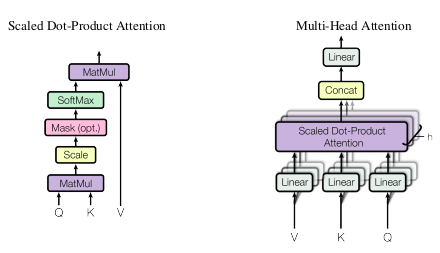
\includegraphics[width=0.75\linewidth]{images/transformer_attention.png}
  \caption{Self-attention pipeline: query--key similarity produces data-dependent mixing of values (adapted from Vaswani et al., 2017~\cite{vaswani2017attention}).}
  \label{fig:transformer_attention}
\end{figure}
\FloatBarrier

% =====================================================
\section{Vision Transformers (ViT)}
\label{sec:lit_vit}

The Vision Transformer (ViT)~\cite{dosovitskiy2020vit} treats an image as a sequence of non-overlapping $P{\times}P$ patches that act as tokens.
Each patch is linearly projected and combined with positional embeddings before passing through stacked transformer encoders.
A [CLS] token aggregates global information for classification.
ViT removes locality bias and allows any patch to attend to any other, thereby capturing long-range dependencies such as fog gradients or underwater scattering that are critical for environmental style modelling.

\begin{figure}[!htbp]
  \centering
  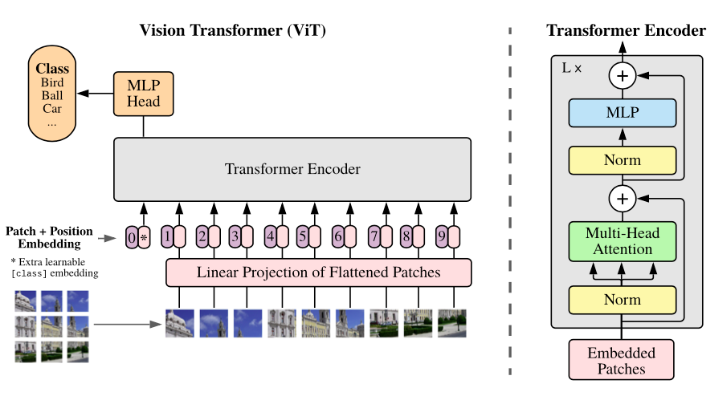
\includegraphics[width=0.75\linewidth]{images/vit_pipeline.png}
  \caption{ViT pipeline and Transformer Block (adapted from Dosovitskiy et al., 2021~\cite{dosovitskiy2020vit}).}
  \label{fig:vit_pipeline}
\end{figure}
\FloatBarrier

% =====================================================
\section{Adaptive Fourier Neural Operators (AFNO)}
\label{sec:afno}

Fourier Neural Operators (FNOs) are used for token mixing in the frequency domain.
Adaptive Fourier Neural Operators (AFNO)~\cite{guibas2021afno} extend FNOs by transforming feature representations to the spectral domain via the Fast Fourier Transform (FFT), which can efficiently model global interactions through operations in frequency space, rather than traditional self-attention mechanisms that are performed directly on spatial tokens.

\noindent The main idea behind AFNO is that many visual patterns are more compactly represented in the frequency domain.
Instead of manipulating individual spatial tokens, AFNO manipulates frequency coefficients to capture long-range dependencies with dramatically reduced computational complexity.
This property has made AFNO effective in large-scale vision tasks, image restoration, weather forecasting, and scientific machine learning applications.

\noindent Given an input feature representation $X \in \mathbb{R}^{H \times W \times C}$, AFNO first maps the feature map to the Fourier domain by a two-dimensional Fourier transform:
\begin{equation}
    \hat{X} = \mathcal{F}(X),
\end{equation}
where $\mathcal{F}(\cdot)$ is the Fourier transform operation.
The transformed coefficients are then spectrally filtered --- with hard-thresholding and soft-shrinkage enforcing sparsity across frequency modes --- and the representation is transformed back to the spatial domain with the inverse Fourier transform.

\noindent One key advantage of AFNO is the ability to model the global structure of images via frequency-space interactions.
Since atmospheric degradations such as haze, fog, smoke, and snowfall tend to preserve coarse scene structure while suppressing high-frequency image information, frequency-domain processing provides a natural mechanism for modelling such degradations.
In this thesis, AFNO adapters are inserted into frozen ViT backbones to selectively modulate frequency bands affected by atmospheric corruption without disturbing the pretrained representations.

\begin{figure}[!htbp]
  \centering
  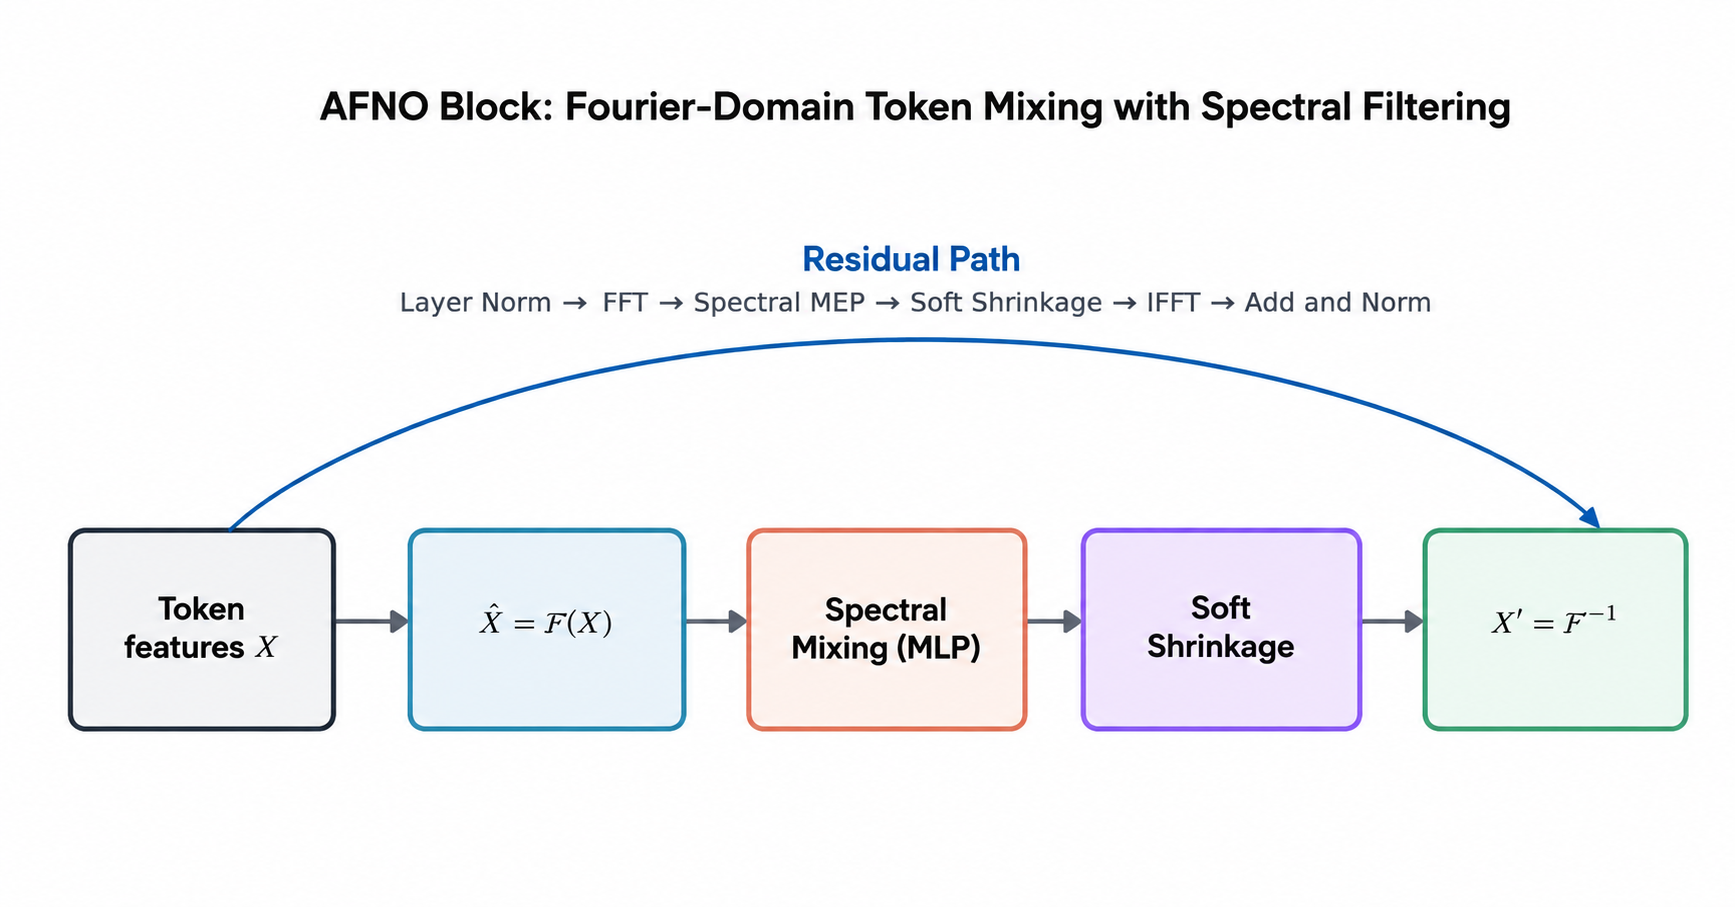
\includegraphics[width=0.92\linewidth]{images/figure_2.3.png}
  \caption{Overview of the Adaptive Fourier Neural Operator (AFNO) block with Fourier-domain token mixing and spectral filtering (adapted from Guibas et al., 2022~\cite{guibas2021afno}).}
  \label{fig:afno}
\end{figure}
\FloatBarrier

\noindent Recent works have shown the effectiveness of AFNO-based architectures for handling large-scale visual transformations and distribution shifts.
The power of AFNO for selective spectral representation manipulation is of particular importance for adaptation under strong atmospheric degradations, where frequency properties differ substantially from those of clean images.

% =====================================================
\section{Generative Adversarial Networks (GANs)}
\label{sec:gans}

\textbf{Generative Adversarial Networks (GANs)}~\cite{goodfellow2014gan} were the first to produce high-fidelity synthetic images.
They train a Generator $G$ and Discriminator $D$ in an adversarial loop:
\[
\min_G \max_D
\mathbb{E}_{x\sim p_\text{data}}[\log D(x)]
+\mathbb{E}_{z\sim p_z}[\log(1-D(G(z)))].
\]
GANs introduced sampling from a learned distribution rather than memorising examples, but adversarial training often causes instability and mode collapse.
Variants such as WGAN~\cite{arjovsky2017wassersteingan} and StyleGAN~\cite{karras2019stylegan} improved visual realism; however, they lacked semantic control and physical interpretability.
The PatchGAN discriminator from Isola et al.~\cite{isola2017image2image} classifies $N\times N$ image patches rather than the full image, and is reused in KDA-Net's haze-authenticator sub-network (Chapter~\ref{chap:phase2_pipeline}).

\begin{figure}[!htbp]
  \centering
  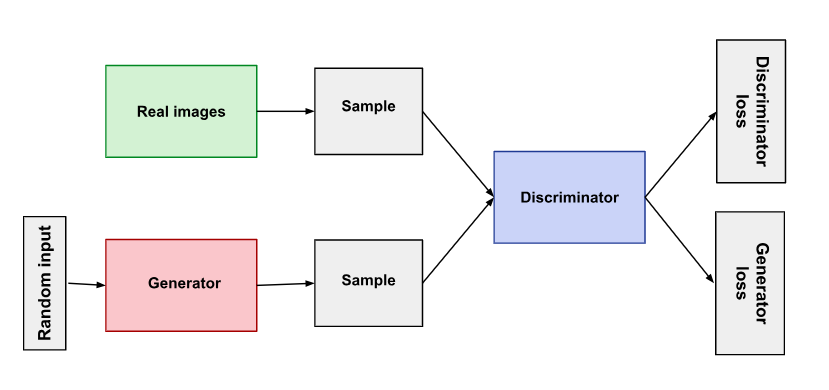
\includegraphics[width=0.72\linewidth]{images/gan_architecture.png}
  \caption{GAN architecture: generator--discriminator adversarial training loop (adapted from Foster, 2023~\cite{foster2023generativedeeplearning}).}
  \label{fig:gan_architecture}
\end{figure}
\FloatBarrier

% =====================================================
\section{Variational Autoencoders (VAEs)}
\label{sec:vaes}

VAEs~\cite{kingma2013autoencoding} model data generation via a continuous latent variable $z$.
They maximise the Evidence Lower Bound (ELBO):
\[
\log p_\theta(x) \ge
\mathbb{E}_{q_\phi(z|x)}[\log p_\theta(x|z)]
- \mathrm{KL}\!\big(q_\phi(z|x)\|p(z)\big),
\quad
z = \mu_\phi(x) + \sigma_\phi(x)\odot\epsilon.
\]
VAEs yield smooth, interpretable latent manifolds enabling continuous interpolation between images.
Although outputs can appear slightly blurred, VAEs provide stability and differentiable latent sampling --- properties later exploited in Latent Diffusion Models (LDMs)~\cite{rombach2022ldm}.

\begin{figure}[!htbp]
  \centering
  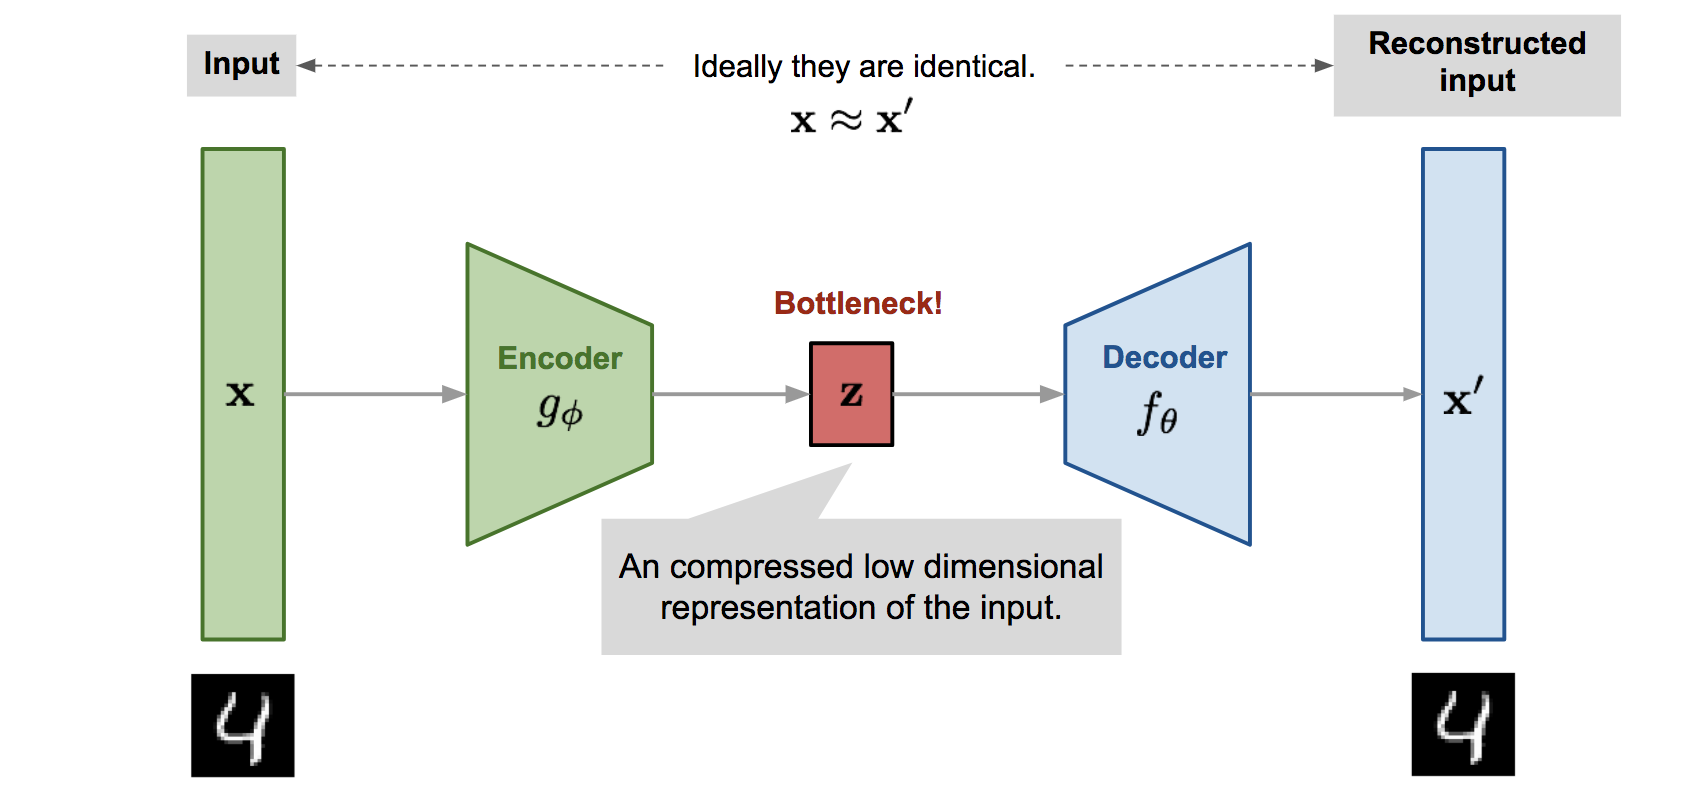
\includegraphics[width=0.75\linewidth]{images/vae_architecture.png}
  \caption{Variational Autoencoder: encoder--decoder with reparameterisation trick (adapted from Foster, 2023~\cite{foster2023generativedeeplearning}).}
  \label{fig:vae_architecture}
\end{figure}
\FloatBarrier

% =====================================================
\section{U-Net Backbone for Diffusion}
\label{sec:lit_unet}

U-Net~\cite{ronneberger2015unet} provides hierarchical feature extraction through an encoder--decoder architecture with skip connections that preserve fine detail.
Diffusion models augment U-Net with \textbf{time-step embeddings} (representing noise level) and \textbf{cross-attention layers} (for text or image conditions), forming the structural engine of modern denoising diffusion.
The encoder progressively downsamples the noisy image into coarse latent features capturing global semantics, while the decoder reconstructs spatial details through upsampling.
Skip connections ensure that high-frequency information from the encoder is passed directly to the corresponding decoder stage.
Time-step embeddings allow the model to adjust its denoising strength dynamically --- focusing on coarse structure during early steps and fine details in later stages.
Cross-attention integrates contextual guidance, enabling the model to align visual content with prompts, reference styles, or other conditioning inputs.

\begin{figure}[!h]
  \centering
  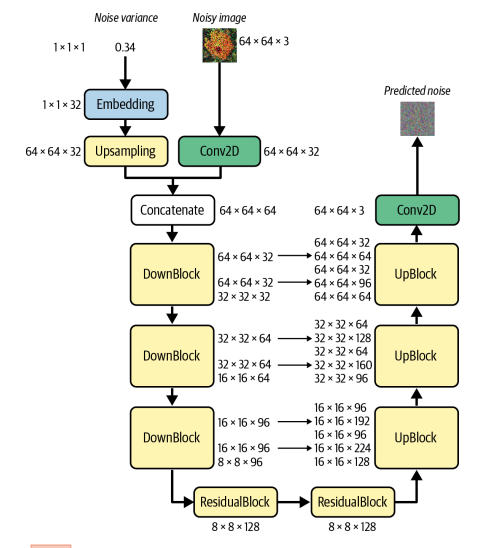
\includegraphics[width=0.60\linewidth]{images/unet_architecture.png}
  \caption{Diffusion U-Net: encoder--decoder with skip connections, time-step embeddings, and cross-attention (adapted from Foster, 2023~\cite{foster2023generativedeeplearning}).}
  \label{fig:unet_architecture}
\end{figure}
\FloatBarrier

% =====================================================
\section{Diffusion Models}
\label{sec:diffusion_models}

Diffusion models~\cite{ho2020ddpm} constitute a family of generative models that gradually convert pure noise into structured data through a learned denoising process, interpreting image generation as the reversal of a stochastic diffusion process.

\subsection*{Forward Process}

The forward process progressively destroys image structure by adding Gaussian noise over $T$ timesteps according to a variance schedule $\{\beta_t\}_{t=1}^T$:
\[
q(x_t|x_{t-1})=\mathcal{N}\big(\sqrt{1-\beta_t}\,x_{t-1},\,\beta_t I\big), \qquad
x_t = \sqrt{\bar{\alpha}_t}\,x_0 + \sqrt{1-\bar{\alpha}_t}\,\epsilon,
\quad \bar{\alpha}_t = \prod_{i=1}^t (1-\beta_i).
\]
As $t\!\to\!T$, $x_T$ approaches pure noise.

\begin{figure}[!htbp]
  \centering
  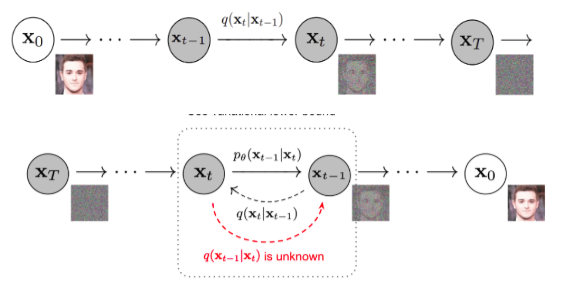
\includegraphics[width=0.75\linewidth]{images/ddpm_forward_reverse.png}
  \caption{Forward and reverse diffusion: corruption by Gaussian noise and stepwise denoising (adapted from Foster, 2023~\cite{foster2023generativedeeplearning}).}
  \label{fig:diffusion_process}
\end{figure}
\FloatBarrier

\subsection*{Reverse Process}

A neural network $\epsilon_\theta(x_t,t)$ is trained to predict the noise at each timestep:
\[
p_\theta(x_{t-1}|x_t)
=\mathcal{N}\!\big(\mu_\theta(x_t,t),\,\sigma_t^2 I\big), \quad
\mathcal{L}_{\text{simple}}
=\mathbb{E}_{x_0,t,\epsilon}
\big[\|\epsilon-\epsilon_\theta(\sqrt{\bar{\alpha}_t}x_0+\sqrt{1-\bar{\alpha}_t}\epsilon,t)\|^2\big].
\]
At inference, the process begins from $x_T\!\sim\!\mathcal{N}(0,I)$ and iteratively denoises until $x_0$ emerges.
DDIM~\cite{song2021ddim} reformulates this as a non-Markovian process enabling deterministic sampling in 40--50 steps rather than 1000, and is the inference scheduler used throughout this work.

\subsection*{Conditional and Guided Diffusion}
\label{sec:conditional_diffusion}

An external classifier $p_\phi(y|x_t)$ can guide sampling by adjusting the predicted noise~\cite{dhariwal2021diffusion}:
\[
\tilde{\epsilon}_\theta(x_t,t|y)
=\epsilon_\theta(x_t,t)
- w\,\sigma_t\nabla_{x_t}\log p_\phi(y|x_t).
\]
Modern diffusion integrates conditioning directly inside the U-Net via cross-attention, with $(K,V)$ from conditioning encoders (text or style) and $Q$ from U-Net activations.

\subsection*{Latent Diffusion and Stable Diffusion}
\label{sec:ldm_stable}

Latent Diffusion Models (LDMs)~\cite{rombach2022ldm} perform diffusion in the latent space of a pretrained VAE, drastically reducing computation.
SDXL~\cite{podell2023sdxlimprovinglatentdiffusion} extends this with dual-encoder text conditioning (CLIP ViT-L/14 + OpenCLIP ViT-bigG) at $1024\times1024$ native resolution.
It is the generative backbone for all experiments in this work.

\begin{figure}[!htbp]
  \centering
  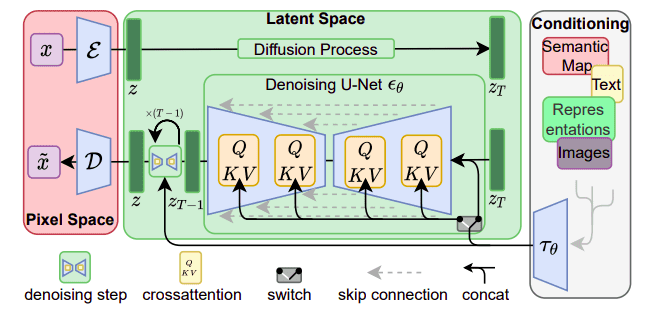
\includegraphics[width=0.7\linewidth]{images/stable_diffusion_architecture.png}
  \caption{Stable Diffusion: text-conditioned latent denoising within a VAE encoder--decoder pipeline (adapted from Foster, 2023~\cite{foster2023generativedeeplearning}).}
  \label{fig:stable_diffusion}
\end{figure}
\FloatBarrier

% =====================================================
\section{CLIP Encoders and Vision-Language Models}
\label{sec:clip}

Vision-language models have become a powerful paradigm for learning generalised visual representations with large-scale multimodal pretraining.
Instead of depending on manually annotated class labels, these models learn aligned representations between images and natural language descriptions that can be effectively transferred to a wide range of downstream tasks.

\noindent Contrastive Language-Image Pretraining (CLIP)~\cite{radford2021clip} is one of the most influential vision-language models.
CLIP has two independent encoders: an image encoder and a text encoder.
During training, images and text are projected into a common embedding space using a contrastive objective that pulls similar pairs together and pushes apart dissimilar pairs.

\noindent Let $I$ denote an image and $T$ its corresponding text description.
CLIP learns image and text embeddings:
\begin{equation}
    z_I = f_I(I), \qquad z_T = f_T(T),
\end{equation}
where $f_I$ and $f_T$ are the image and text encoders respectively.
The cosine similarity between the embeddings is:
\begin{equation}
    s(I,T) = \frac{z_I \cdot z_T}{\|z_I\|\,\|z_T\|}.
\end{equation}
This formulation allows zero-shot classification by matching image embeddings with textual descriptions of candidate categories.
Training uses the InfoNCE loss:
\[
\mathcal{L}_{\text{CLIP}}
=-\frac{1}{N}\sum_{i=1}^N
\Big[
\log\frac{e^{s(I_i,T_i)/\tau}}{\sum_j e^{s(I_i,T_j)/\tau}}
+\log\frac{e^{s(I_i,T_i)/\tau}}{\sum_j e^{s(I_j,T_i)/\tau}}
\Big].
\]

\begin{figure}[!htbp]
  \centering
  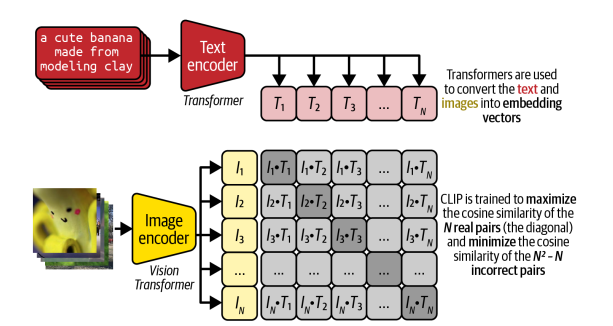
\includegraphics[width=0.65\linewidth]{images/clip_contrastive.png}
  \caption{CLIP architecture with separate image and text encoders trained with contrastive learning (adapted from Foster, 2023~\cite{foster2023generativedeeplearning}).}
  \label{fig:clip_contrastive}
\end{figure}
\FloatBarrier

\noindent CLIP's large-scale pretraining paradigm has proven remarkably robust and transferable to a wide range of visual tasks.
However, it is well established that severe environmental degradations can still impact the quality of its representations, motivating the adaptation strategies developed in this thesis.

% =====================================================
\section{Contrastive Style Descriptors (CSD)}
\label{sec:csd}

The success of large-scale vision-language models has generated growing interest in learning representations that separate semantic content from visual style.
Semantic representations describe the objects and structure of an image, while style representations describe attributes such as texture, colour distribution, illumination, atmospheric conditions, and artistic characteristics.
Properly disentangling these factors is of great value for controllable image synthesis and style-guided generation.

\noindent Conventional style transfer methods generally depend on low-level feature statistics extracted from convolutional neural networks.
Such representations capture texture information but often fail to provide robust semantic understanding of style across different image domains.
Recent works have therefore explored contrastive learning approaches for learning more sophisticated style representations directly from large-scale visual datasets.

\noindent Contrastive Style Descriptors (CSD)~\cite{somepalli2024measuring} offer a framework for learning disentangled representations of style and content via contrastive learning.
CSD builds upon frozen CLIP encoders, where different projection heads learn style-aware and content-aware representations while preserving the semantic knowledge learned in the CLIP feature space.

\noindent Given an image representation $z$ extracted from a pretrained CLIP encoder, CSD learns separate style and content mappings:
\begin{equation}
    z_s = f_s(z), \qquad z_c = f_c(z),
\end{equation}
where $f_s$ and $f_c$ are style and content projection functions respectively.
The goal is to have images with similar stylistic characteristics be close to each other in the style embedding space while being well separated from semantically different styles.
This is achieved using contrastive objectives that maximise agreement between positive style pairs and minimise similarity between negative pairs.
Similarity is computed as:
\[
\mathrm{Sim}(x_g, x_r) = \frac{z_g^\top z_r}{\|z_g\|\,\|z_r\|}.
\]


\noindent This results in style representations that semantically describe atmospheric characteristics such as haze, snow, smoke, and sandstorms.
Contrastive style descriptors are more robust and better match human perception of environmental appearance than traditional texture-statistics-based style representations.

\noindent The ability to measure stylistic similarity in a learned embedding space enables new forms of controllable image generation and style-guided diffusion.
In particular, style descriptors can be employed as a guiding signal during the diffusion process, steering generated samples towards desired atmospheric characteristics while preserving scene structure.

\begin{figure}[htbp]
    \centering
    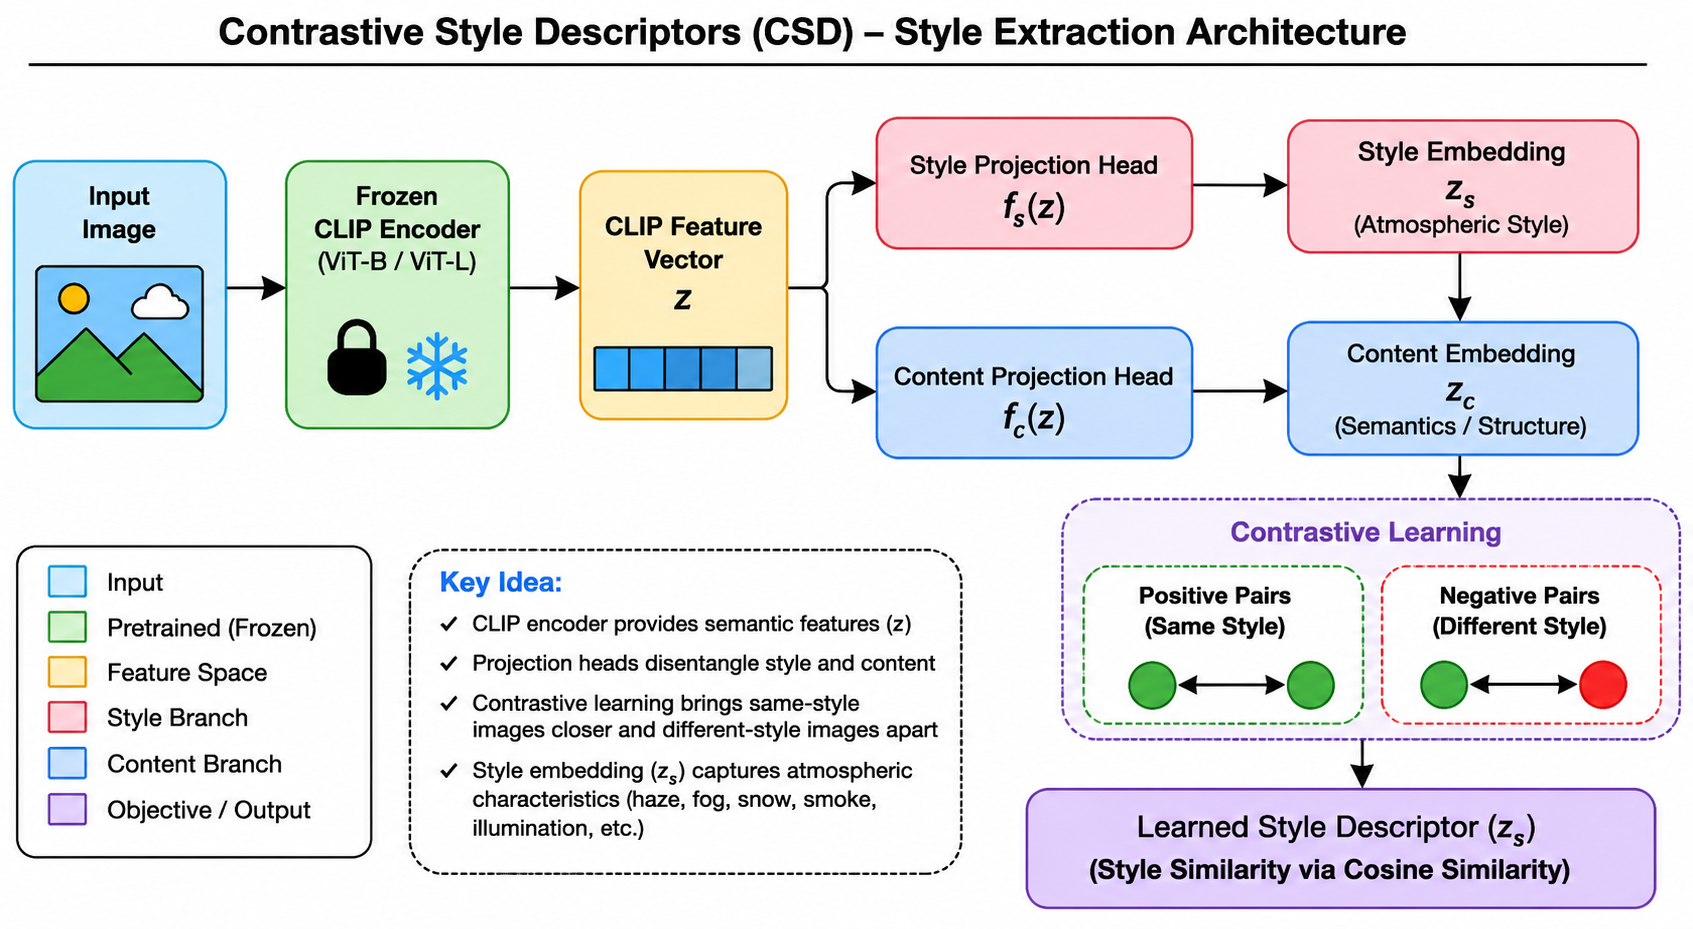
\includegraphics[width=0.85\linewidth]{images/CSD_Architecture.png}
    \caption{CSD architecture. A frozen CLIP encoder produces a shared representation $z$, projected by separate style ($f_s$) and content ($f_c$) heads trained with contrastive objectives. The disentangled style embedding yields the similarity $\mathrm{Sim}(x_g, x_r)$ used as a style-guidance signal during denoising.}
    \label{fig:csd_architecture}
\end{figure}

% =====================================================
\section{Adapters, Structural Guidance, and Prompt Fusion}
\label{sec:adapters_control}

Adapters add modular control to pretrained diffusion models without retraining the backbone.

\subsection{ControlNet}
\label{sec:controlnet}

Zhang et al.~\cite{zhang2023controlnet} introduced ControlNet, which adds a zero-initialised side network that processes structural cues (edges, depth, segmentation) and merges them back into the U-Net via additive connections.
The side network mirrors the U-Net encoder layers; zero initialisation ensures the model begins as an exact copy of the base diffusion system and gradually learns to incorporate external structure only when relevant, preventing training instability.
Multiple conditioning types can be fused simultaneously, enabling precise and interpretable spatial control.
InstantStyle-Plus (Chapter~\ref{chap:adaptive_proposed}) uses Tile ControlNet for spatial structure preservation during style transfer.

\begin{figure}[!htbp]
  \centering
  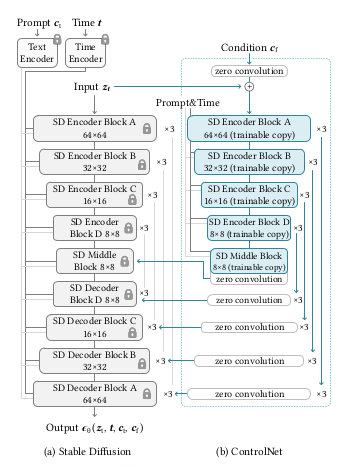
\includegraphics[width=0.7\linewidth]{images/controlnet_architecture.png}
  \caption{ControlNet: structure encoder merged into U-Net via additive connections (adapted from Zhang et al., 2023~\cite{zhang2023controlnet}).}
  \label{fig:controlnet_architecture}
\end{figure}
\FloatBarrier

\subsection{T2I-Adapter}
\label{sec:t2i_adapter}

Mou et al.~\cite{mou2024t2i} introduced T2I-Adapter, which provides lightweight structural conditioning through small adapter modules trained to align external guidance signals (sketch, depth, colour) with the internal feature space of a frozen text-to-image diffusion model.
Unlike ControlNet, T2I-Adapter uses a separate compact encoder rather than a full copy of the U-Net, significantly reducing the number of additional parameters while achieving comparable spatial controllability.

\subsection{IP-Adapter}
\label{sec:ip_adapter}

Ye et al.~\cite{ye2023ipadapterfidelityadapters} introduced IP-Adapter, which injects style from a reference image via decoupled cross-attention alongside text embeddings.
InstantStyle~\cite{wang2024instantstyle} demonstrated that style and spatial structure are not uniformly distributed across U-Net blocks --- \texttt{up\_blocks.0} and \texttt{up\_blocks.1} carry style information while remaining blocks carry layout and semantic content.
By restricting IP-Adapter injection to only these style blocks, InstantStyle achieves style injection without layout transfer.
InstantStyle-Plus~\cite{wang2024instantstyleplus} further extends this with Tile ControlNet for layout-preserving style transfer when a content image is available.
Text dictates \emph{what} to draw; the reference image defines \emph{how} it should appear --- controlling tone, colour, and texture without disturbing geometry.

\begin{figure}[!htbp]
  \centering
  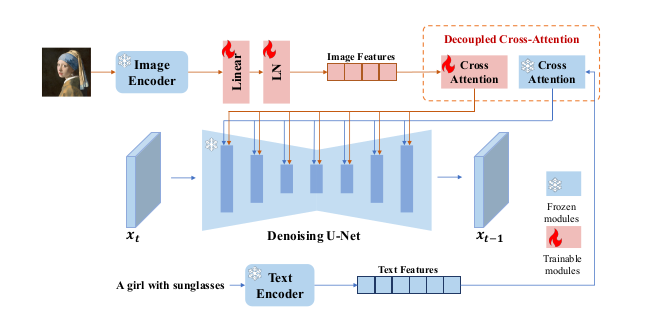
\includegraphics[width=0.7\linewidth]{images/ip_adapter_architecture.png}
  \caption{IP-Adapter: decoupled attention merges text semantics and image-based style cues (adapted from Ye et al., 2023~\cite{ye2023ipadapterfidelityadapters}).}
  \label{fig:ip_adapter_architecture}
\end{figure}
\FloatBarrier

% =====================================================
\section{Optimization-Guided Diffusion}
\label{sec:opt_guided_diffusion}

In a diffusion model, images are generated by iteratively denoising an image, gradually converting noise to structure.
Traditional diffusion models primarily use textual conditioning and cross-attention mechanisms, but recent studies have explored the direct incorporation of external objectives into the denoising trajectory.
These methods, referred to as optimization-guided diffusion, exploit additional guidance signals to steer the reverse diffusion process and direct generated samples towards desired properties.

\noindent Optimization-guided diffusion extends the controllability of diffusion models beyond standard prompt conditioning by using gradients from auxiliary objectives.
Such objectives can be class labels, semantic attributes, style descriptors, perceptual similarity measures, or task-specific constraints.
These approaches provide a flexible framework to control generation by modifying the denoising trajectory during sampling, without the need to retrain the model.

\subsection{Classifier Guidance}

One of the first approaches suggested for controllable diffusion generation was classifier guidance~\cite{dhariwal2021diffusion}.
The basic idea is to use an external classifier to provide gradients that help generated samples conform to a desired target class.
During reverse diffusion, the score estimate is modified with the gradient of the classifier log-probability:
\begin{equation}
    \nabla_{x_t} \log p(x_t \mid y) = \nabla_{x_t} \log p(x_t) + w\,\nabla_{x_t} \log p(y \mid x_t),
\end{equation}
where $y$ is the target condition, $w$ controls the strength of guidance, and $x_t$ is the noisy sample at timestep $t$.
Classifier guidance improves controllability and sample fidelity significantly, but requires training an additional classifier robust to noisy intermediate states, which increases computational complexity and limits practical usability.

\subsection{Classifier-Free Guidance (CFG)}

Classifier-Free Guidance trains conditional and unconditional diffusion models jointly to eliminate the need for an auxiliary classifier.
At inference time, the final score estimate is a combination of the conditional and unconditional predictions:
\begin{equation}
    \hat{\epsilon}_{\mathrm{CFG}} = \epsilon_{\mathrm{uncond}} + s\,\bigl(\epsilon_{\mathrm{cond}} - \epsilon_{\mathrm{uncond}}\bigr),
\end{equation}
where $s$ is the guidance scale.
In modern diffusion systems such as Stable Diffusion and SDXL~\cite{podell2023sdxlimprovinglatentdiffusion}, CFG has become the de-facto guidance mechanism.
The guidance scale can be adjusted to control the trade-off between prompt adherence and image diversity.

\subsection{Stable Diffusion with Constraints}

Recent work has explored embedding explicit constraints into diffusion sampling.
Constrained Stable Diffusion uses an optimization-based guidance to enforce desired properties during generation without additional model training.
The general constrained sampling problem is:
\begin{equation}
    \min_{x}\; f(x) \quad \text{subject to} \quad g(x) \le 0,
\end{equation}
where $f(x)$ is the diffusion objective and $g(x)$ is a user-defined constraint.
A projection and correction step during reverse diffusion produces a process that satisfies perceptual, semantic, or stylistic constraints, providing a principled approach to integrate external guidance signals while preserving the generative capabilities of the pretrained model.

\subsection{Langevin Dynamics}

Langevin dynamics is a stochastic optimization method commonly applied in Bayesian inference and probabilistic sampling.
It combines gradient-based updates with random perturbations, allowing samples to explore complex probability distributions while gradually moving toward regions of high probability.
The standard Langevin update is:
\begin{equation}
    x_{t+1} = x_t + \gamma_t\,\nabla \log p(x_t) + \sqrt{2\gamma_t}\,\epsilon_t, \qquad \epsilon_t \sim \mathcal{N}(0,I),
\end{equation}
where $\gamma_t$ is the step size.
The interplay between deterministic gradient ascent and stochastic exploration allows Langevin dynamics to escape poor local optima and converge to desired distributions.

\subsection{Proximal Langevin Dynamics}

Proximal Langevin Dynamics~\cite{zampini2025constrained} generalises classical Langevin sampling to optimization problems with explicit constraints or non-differentiable regularisation terms.
Instead of direct gradient updates, proximal operators project intermediate solutions onto feasible sets defined by the constraints:
\begin{equation}
    x_{t+1} = \mathrm{prox}_{\lambda g}\!\left(x_t + \gamma_t\,\nabla \log p(x_t) + \sqrt{2\gamma_t}\,\epsilon_t\right),
\end{equation}
where $\mathrm{prox}_{\lambda g}$ denotes the proximal operator of constraint function $g$.
This formulation provides a mathematically principled way to incorporate constraints into stochastic sampling procedures.
Chapter~\ref{chap:csd_style} evaluates this approach with CSD similarity as the constraint function; the trial experiments chapter applies it with AFNO style features.
In practice, gradient instability through the VAE decoder and sensitivity to the convergence threshold limit its scalability.

% =====================================================
\section{Physics-Based Atmospheric Image Formation}
\label{sec:atmospheric_physics}

Light interacting with particles suspended in the atmosphere creates atmospheric phenomena such as haze, fog, smoke, and dust.
These effects follow well-established physical processes --- scattering, absorption, and transmission --- unlike purely appearance-based image transformations.
Physics-based image formation models therefore provide a principled means of simulating atmospheric degradations and their impact on visual perception.

\subsection{Atmospheric Scattering Theory}

Some of the incident radiance is either scattered or absorbed by a participating medium before it reaches the camera as light propagates through it.
The extent of attenuation depends on particle density, viewing distance, and wavelength of light, leading to decreased visibility, contrast degradation, and colour shifts characteristic of adverse weather conditions.

\noindent Atmospheric image formation is commonly represented as the sum of two components: attenuated scene radiance and airlight.
The attenuated radiance is the light from scene objects that arrives at the camera after transmission through the atmosphere.
Airlight is the scattered environmental illumination accumulated along the viewing path.

\subsection{Koschmieder Model}

The Koschmieder model~\cite{koschmieder1924theorie} is one of the most commonly used models for atmospheric scattering and describes image formation under homogeneous atmospheric conditions.
The observed image intensity is:
\begin{equation}
    I(x) = J(x)\,T(x) + A\,\bigl(1-T(x)\bigr),
\end{equation}
where $I(x)$ is the observed image, $J(x)$ is the scene radiance, $A$ is the global atmospheric light, and $T(x)$ is the transmission map.
The transmission map is defined as:
\begin{equation}
    T(x) = e^{-\beta\, d(x)},
\end{equation}
where $\beta$ is the atmospheric extinction coefficient and $d(x)$ is the scene depth.
The model captures two major atmospheric effects: attenuation of scene radiance and accumulation of scattered atmospheric light.
As depth increases, transmission decreases, resulting in reduced visibility and stronger atmospheric effects.
The physics-grounded synthesis pipeline (Chapter~\ref{chap:phase2_pipeline}) uses the Koschmieder model as a depth-consistent compositor.

\begin{figure}[!htbp]
  \centering
  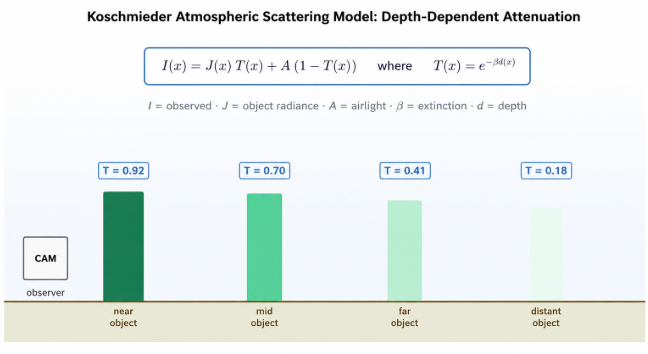
\includegraphics[width=0.92\linewidth]{images/figure_2.13.png}
  \caption{Schematic of atmospheric image formation with the Koschmieder scattering model: foreground objects appear clear while distant objects dissolve into the atmospheric medium.}
  \label{fig:koschmieder}
\end{figure}
\FloatBarrier

\subsection{Dark Channel Prior}

The Dark Channel Prior (DCP)~\cite{he2009dark} is a widely used technique for estimating atmospheric transmission from a single image.
The method is based on the observation that most natural outdoor images contain pixels with very low intensity values in at least one colour channel.
This property is exploited to estimate atmospheric light and transmission maps without requiring depth information.
Originally introduced for image dehazing, DCP has become an important tool for understanding atmospheric image formation and visibility degradation.
In the physics-grounded synthesis pipeline, the DCP is used to estimate per-domain $\beta$ and $A$ values from reference atmospheric photographs.

\subsection{Monocular Depth Estimation}

In atmospheric scattering models, depth is the main factor, as the degree of degradation is proportional to the distance of the object.
With recent progress in transformer-based depth estimation, accurate monocular depth estimation from a single RGB image is now feasible.
Methods such as MiDaS and DPT (Dense Prediction Transformers)~\cite{ranftl2021dpt} leverage large-scale pretraining and transformer architectures to predict dense depth maps across diverse environments.
These depth estimates can be combined with atmospheric scattering models to generate physically consistent, scene-geometry-dependent degradations.

\noindent By combining depth estimation and atmospheric scattering models, a physics-based framework for synthesising environmental effects is obtained.
In contrast to purely appearance-based stylisation approaches, depth-aware atmospheric formation explicitly models the attenuation of visibility and the degradation of the environment with respect to distance, enabling more realistic and controllable environmental transformations.
In the physics-grounded synthesis pipeline, DPT-Large depth maps drive the transmission map $T(x)$ computation for the Koschmieder compositor.

% =====================================================
\section*{Summary}

Research has steadily advanced toward controllable and interpretable generation.
Transformers introduced attention mechanisms; ViTs extended them to vision; GANs and VAEs pioneered generative modelling.
Diffusion unified these ideas into a stable probabilistic framework, enhanced by latent conditioning, cross-attention, and adapters such as ControlNet, T2I-Adapter, and IP-Adapter.
AFNO provides frequency-domain adaptation for frozen ViT backbones, enabling efficient correction for atmospheric distribution shifts.
Contrastive systems such as CLIP and CSD add semantic and stylistic grounding, while physics-based Koschmieder compositing provides the final layer of physical realism.
Together, these components form the complete methodological foundation of the work presented in the following chapters.

% =====================================================
\chapter{Preliminary Experiments and Baseline Evaluation}
\label{chap:foundations_existing}

This chapter covers two preparatory stages of the research.
The first is a series of foundational experiments --- Vision Transformer, U-Net, DDPM, and classifier-guided conditional diffusion --- carried out to build an intuitive understanding of the key components that drive diffusion-based generative models.
The intent was not to reproduce benchmark-level results but to practically observe how different architectures behave once trained: how the loss evolves, how reconstruction emerges from noise, and how conditioning mechanisms influence the generation process.
The second stage is a systematic evaluation of three state-of-the-art style-transfer frameworks (StyleShot, CSGO, and InstantStyle) against a curated dataset of extreme-weather reference imagery.
This evaluation establishes the performance ceiling of off-the-shelf methods and identifies the precise failure mode --- physically incoherent atmospheric rendering --- that the proposed system in Chapter~\ref{chap:adaptive_proposed} was designed to address.

% =====================================================
\section{Foundational Experiments}
\label{sec:foundations}

\noindent Before engaging with any existing framework, time was spent implementing and observing the underlying building blocks from scratch.
Each experiment captures one essential property of diffusion systems: ViT illustrates the power of attention in capturing global context; U-Net demonstrates how spatial structure is preserved through skip connections; DDPM visualizes the transformation from noise to structure; and classifier-guided diffusion introduces controllability through explicit gradient-based conditioning.
Together, they form the conceptual and empirical foundation upon which later adaptive and style-aware diffusion experiments are built.

% -------------------------------------------------------
\subsection{Vision Transformer (ViT)}
\label{sec:vit}

\noindent The Vision Transformer (ViT)~\cite{dosovitskiy2020vit} experiment was designed to understand how transformer-based vision models capture global relationships in images compared to convolutional architectures.
A compact ViT with a shallow DETR-style~\cite{carion2020endtoendobjectdetectiontransformers} head was implemented to explore how patch embeddings interact with query-based decoding.
Training was performed on CIFAR-10, with images resized to $224\times224$ to fit the patch embedding scheme.
The setup used the Adam optimiser ($3\times10^{-4}$), batch size 64, and 50 epochs of training with ReLU activation and 0.1 dropout.
The network used a 768-dimensional embedding space, 12 attention heads, and a patch size of 16.

DETR (Detection Transformer)~\cite{carion2020endtoendobjectdetectiontransformers} was originally introduced to remove handcrafted detection stages such as anchor boxes or non-maximum suppression, relying solely on attention to perform end-to-end object detection.
It formulates detection as a direct set prediction task using the Hungarian loss for optimal bipartite matching between predicted and ground-truth objects.
In this experiment, while detection itself was not the goal, integrating the DETR-style decoder provided a practical view of how attention can align semantically meaningful tokens, thereby learning structure without explicit convolution.

\paragraph{Results}
The ViT achieved around \textbf{85\% test accuracy} on CIFAR-10.
Attention visualisations clearly revealed that transformer heads concentrated on key object parts (e.g., airplane wings or vehicle bodies) while ignoring background clutter.
Training was smooth, with stable convergence by the 40th epoch.
The experiment reinforced the interpretability and global reasoning capacity of attention, thereby forming the mental framework used later to understand cross-attention in diffusion models.

\begin{figure}[!h]
    \centering
    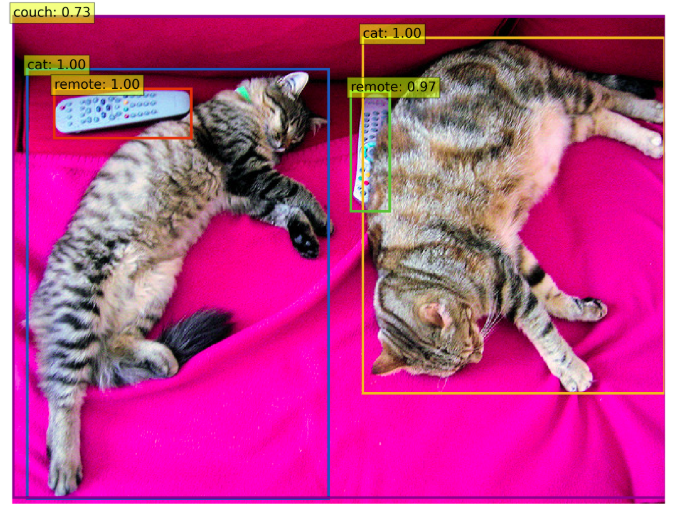
\includegraphics[width=0.65\linewidth]{images/vit_results.png}
    \caption{Vision Transformer on CIFAR-10: attention heads highlighting key semantic regions.}
    \label{fig:vit_results}
\end{figure}

% -------------------------------------------------------
\subsection{U-Net Backbone}
\label{sec:unet}

\noindent The U-Net~\cite{ronneberger2015unet} backbone was explored to understand how skip connections preserve fine structure during reconstruction --- a feature that makes it the default denoising network in diffusion models.
A basic U-Net autoencoder was trained on the Oxford-IIIT Pet dataset ($128\times128$ resolution) for segmentation using Adam ($1\times10^{-3}$), cross-entropy loss, and batch size 8.
Each encoder block contained two $3\times3$ convolutions with ReLU followed by max pooling; the decoder mirrored this with transposed convolutions and symmetric skip connections.
The architecture was intentionally kept simple to focus on reconstruction behaviour rather than architectural sophistication.

\paragraph{Results}
Training converged quickly, with the model accurately recovering spatial boundaries after just a few epochs.
Figure~\ref{fig:unet_segmentation_results} shows clean, sharp segmentation outputs that closely match ground-truth masks.
Skip connections clearly restored high-frequency information lost during downsampling, which explains why the same structure works so effectively in denoising networks.
In diffusion settings, these skip pathways combine with sinusoidal time-step embeddings, giving the model temporal awareness of which stage of denoising it is in and making U-Net both spatially and temporally adaptive.

\begin{figure}[!h]
    \centering
    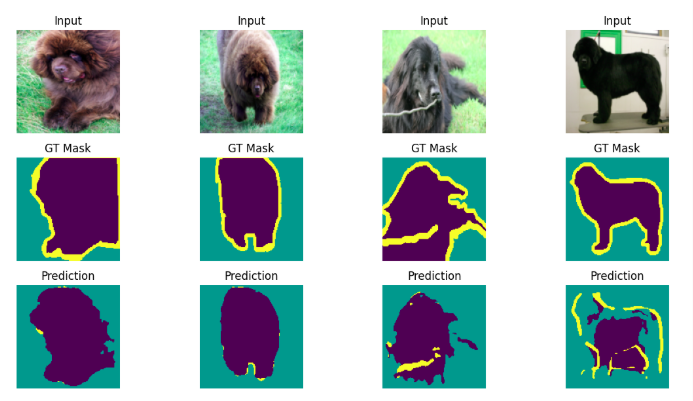
\includegraphics[width=0.55\linewidth]{images/unet_segmentation_results.png}
    \caption{U-Net on Oxford-IIIT Pet: input, ground truth, and reconstructed output.}
    \label{fig:unet_segmentation_results}
\end{figure}

% -------------------------------------------------------
\subsection{Denoising Diffusion Probabilistic Model (DDPM)}
\label{sec:ddpm}

\noindent The DDPM~\cite{ho2020ddpm} experiment visualised the \emph{order from noise} process central to diffusion-based generation.
A U-Net backbone was employed, augmented with sinusoidal time embeddings to encode temporal information.
Training was performed on MNIST (resized to $32\times32$) for 15 epochs using the Adam optimiser ($1\times10^{-4}$) and a linear $\beta_t$ schedule ranging from $1\times10^{-4}$ to $2\times10^{-2}$ over 1000 diffusion steps.
The network learned to predict the clean image $x_0$ from a noisy latent $x_t$ by minimising mean-squared error between the predicted and actual noise.

\paragraph{Results.}
Figure~\ref{fig:ddpm_samples} illustrates the progressive refinement of generated digits.
At the earliest diffusion steps, outputs resemble pure Gaussian noise with no discernible structure.
As sampling proceeds, faint digit contours appear --- a reflection of the model beginning to estimate global shape information.
Midway through the denoising trajectory, the model stabilises coarse structure (loops of 0, stalks of 1 or 9), while fine pixel-level details remain stochastic.
In the final few steps, residual noise is systematically removed, revealing sharply formed digits with clear boundaries and correct topology.

This progression provides an intuitive visualisation of how diffusion models learn to reverse entropy: rather than generating pixels directly, the model gradually transforms a noise distribution into structured data through a sequence of learned conditional transitions.
The experiment also highlights the smooth and interpretable nature of diffusion learning --- unlike GANs~\cite{goodfellow2014gan}, where generation can be abrupt or unstable, diffusion exhibits continuous improvement across time steps, offering clear insight into how the model internalises spatial and probabilistic cues from the dataset.
Despite being trained on a simple dataset, the experiment effectively demonstrates the fundamental mechanics of diffusion, validating the theoretical framework that underpins more advanced models such as Stable Diffusion and InstantStyle.

\begin{figure}[!h]
    \centering
    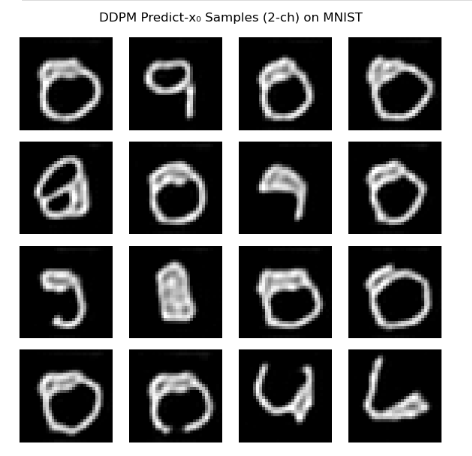
\includegraphics[width=0.65\linewidth]{images/ddpm_samples.png}
    \caption{DDPM on MNIST: progressive denoising from pure noise to clear digits.}
    \label{fig:ddpm_samples}
\end{figure}

% -------------------------------------------------------
\subsection{Conditional Diffusion (Classifier-Guided)}
\label{sec:conditional_diffusion_exp}

\noindent The classifier-guided diffusion setup introduced explicit control into the generative process.
A DDPM denoiser was paired with a CNN~\cite{oshea2015introductionconvolutionalneuralnetworks} classifier trained on noisy MNIST samples to predict class labels at varying noise levels (Adam $1\times10^{-3}$, batch size 128, 10 epochs).
During sampling, gradients from $\nabla_{x_t}\log p_\phi(y|x_t)$ were added to the DDPM mean estimate, scaled by a guidance factor $\lambda=2.0$, thereby steering generation toward the specified target class.

\paragraph{Results}
At lower guidance scales, the model generated diverse samples, whereas higher $\lambda$ values produced sharper and more class-consistent digits at the cost of variety.
The results visually confirmed that classifier gradients can effectively modulate diffusion trajectories --- a precursor to modern conditioning mechanisms such as cross-attention.
This small but powerful experiment completed the conceptual bridge between unconditioned diffusion and controlled, prompt-driven generation.

\begin{figure}[!h]
    \centering
    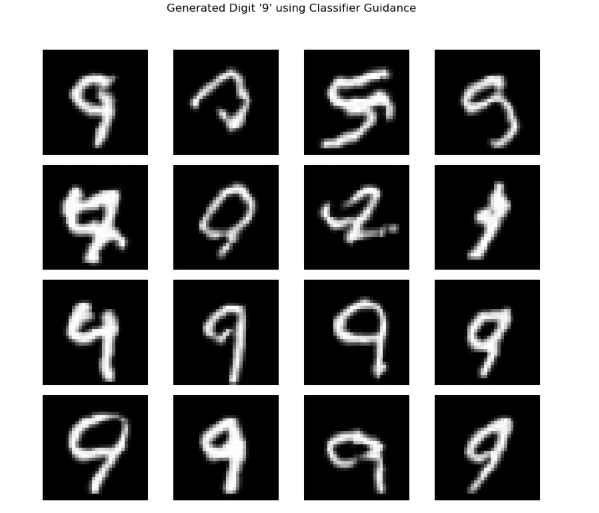
\includegraphics[width=0.65\linewidth]{images/guided_diffusion_results.png}
    \caption{Classifier-Guided Diffusion on MNIST: class `9' generations at guidance scale $\lambda=2.0$.}
    \label{fig:guided_diffusion_results}
\end{figure}

% =====================================================
\section{Dataset for Style-Transfer Evaluation}
\label{sec:dataset}

\noindent Before evaluating any existing style-aware diffusion systems, a focused dataset was curated to represent the kind of distribution shifts observed in the wild.
Approximately \textbf{500 images} were handpicked from publicly available sources such as Pinterest~\cite{pinterest}, iStock~\cite{istock}, and Google Images~\cite{google_images}, spanning a wide range of adverse environmental conditions such as fog, smog, heavy rain, snow, blizzard, sandstorm, dust storm, storm, and forest fire.
These scenes were specifically selected because both the background and foreground elements are often veiled under a strong stylistic ``shroud,'' which makes object boundaries ambiguous and significantly complicates classification and detection tasks.
This dataset serves as the common evaluation ground for all subsequent models.

\noindent \textbf{Note:} Although testing and benchmarking were carried out across all environmental domains mentioned above, the following visual comparisons and analyses focus specifically on the \textbf{agriculture domain}, which was found to most effectively resonate with the objectives of realistic distribution-shift representation and volumetric environmental stylisation.

\begin{figure}[!h]
    \centering
    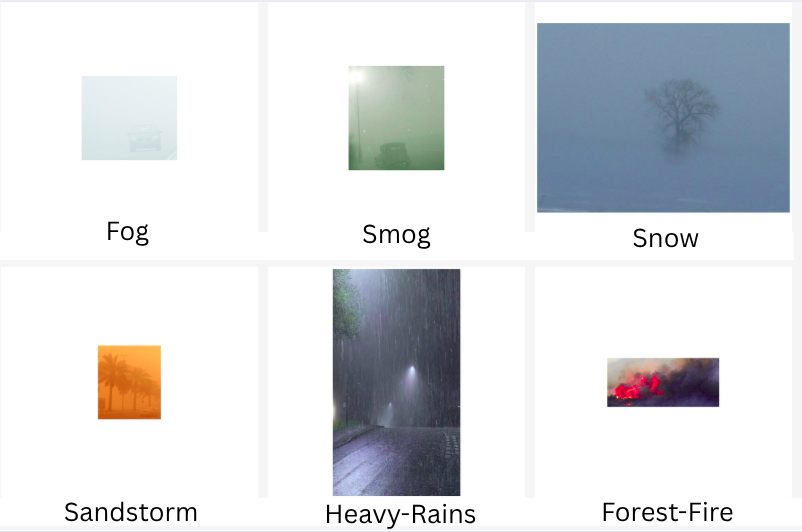
\includegraphics[width=\linewidth]{images/curated_dataset_collage.png}
    \caption{Representative collage from the curated dataset used for evaluation, spanning diverse environmental conditions such as fog, smog, snow, sandstorm, and forest fire. The agriculture domain subset (shown here) was selected for focused visual analysis due to its strong correspondence with real-world visibility and scattering effects.}
    \label{fig:curated_dataset_collage}
\end{figure}

% =====================================================
\section{Evaluation of Existing Style-Transfer Frameworks}
\label{sec:existing_solutions}

\noindent Three frameworks were evaluated in sequence, each representing a different philosophy for injecting style into a pretrained generative model.
The progression --- from auxiliary style network (StyleShot) to encoder-fusion (CSGO) to attention-block selection (InstantStyle) --- tells a story about where style actually lives in a diffusion model.

% -------------------------------------------------------
\subsection{StyleShot: One-Shot Style Transfer with Attention Modulation}
\label{sec:styleshot}

To explore prompt-guided, reference-based style transfer under environmental distribution shifts, the first existing solution evaluated was \textbf{StyleShot}~\cite{gao2024styleshot}.
These scenes were selected to intentionally represent the loss of visibility and structural ambiguity typical of style-induced distribution shifts, where both the background and foreground appear enveloped in a dense ``style shroud.''
The goal was to examine whether the model could convincingly reproduce such styles while maintaining semantic coherence.

\paragraph{Architecture Overview}
As illustrated in Figure~\ref{fig:styleshot_architecture}, the original StyleShot framework is designed as a \textbf{tri-modal diffusion system}, integrating three modalities --- text, content, and style --- into a unified diffusion backbone.
It consists of three encoders:
(1) a \textbf{Style-Aware Encoder} that partitions the style reference image into multiple scales and embeds each partition using transformer blocks (OpenCLIP ViT-H/14)~\cite{radford2021clip} to capture tone, colour, and texture statistics;
(2) a \textbf{Content-Fusion Encoder} that processes edge maps or structure references to maintain spatial layout; and
(3) a \textbf{CLIP Text Encoder} that provides semantic grounding for prompt-based control.
These embeddings are fused within the diffusion U-Net~\cite{ronneberger2015unet} via \textbf{Parallel Cross-Attention} and \textbf{Residual Addition}, enabling the network to modulate appearance (from the style image) while preserving textual and structural semantics.

\begin{figure}[!h]
    \centering
    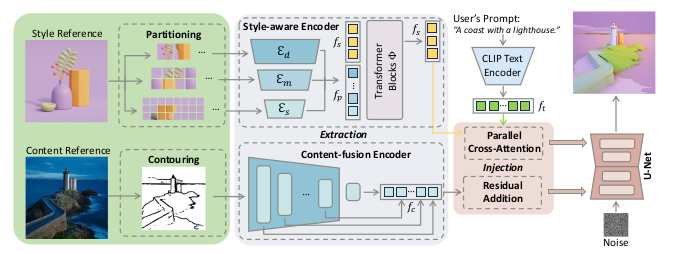
\includegraphics[width=0.75\linewidth]{images/styleshot_architecture.png}
    \caption{Overall architecture of StyleShot~\cite{gao2024styleshot}: tri-modal fusion of style, content, and text embeddings through parallel cross-attention and residual addition in the diffusion U-Net.}
    \label{fig:styleshot_architecture}
\end{figure}

\paragraph{Modified Experimental Configuration}
In this work, the setup was simplified to reflect the \textbf{text + style reference} configuration, as the curated dataset did not include explicit content reference images or edge maps.
Accordingly, the \textit{Content-Fusion Encoder} branch was disabled.
The model thus operated as a \textbf{bi-modal diffusion system}, driven by the CLIP text embeddings for semantic composition and the style-aware embeddings for texture and tone modulation.
The fusion occurred through parallel cross-attention layers within the diffusion U-Net, where style tokens ($f_s$) and text embeddings ($f_t$) jointly influenced the denoising trajectory:
\[
\text{Attn}_{\text{final}} = \text{Attn}(Q, K_t, V_t) + \lambda_s \, \text{Attn}(Q, K_s, V_s),
\]
with $\lambda_s$ controlling the relative style strength.

\paragraph{Results}
When evaluated on the curated dataset, StyleShot~\cite{gao2024styleshot} generated outputs that were visually rich but \textbf{overly artistic} and aesthetically biased rather than physically realistic.
The model often prioritised stylistic exaggeration over faithful reconstruction, producing textures reminiscent of oil painting or digital art.
This deficiency became evident in agricultural and outdoor scenes, where machinery and terrain edges remained sharply defined while the background appeared painterly and abstract.
Similarly, in underwater or snow-heavy conditions, StyleShot was unable to simulate realistic scattering, depth-based attenuation, or backscatter, producing flattened tones that lacked the characteristic absorption and haze structure seen in real imagery.

\begin{figure}[!h]
    \centering
    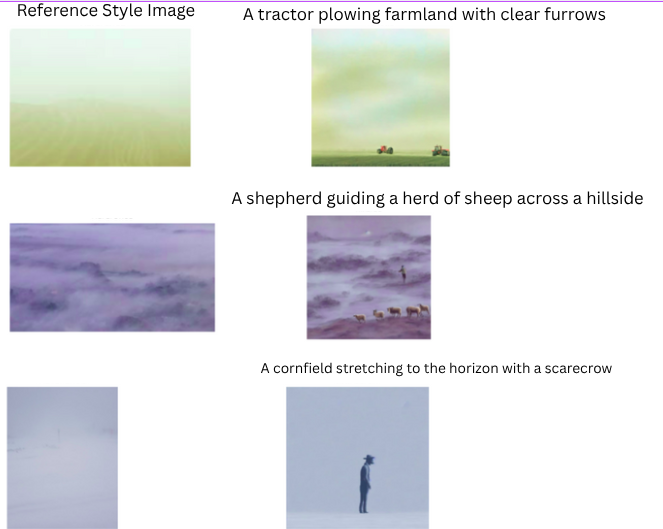
\includegraphics[width=0.85\linewidth]{images/styleshot_fail_agriculture.png}
    \caption{StyleShot on curated agricultural scenes: over-stylisation and lack of depth-consistent haze. Foreground regions remain overly sharp while the background becomes painterly.}
    \label{fig:styleshot_fail_agri}
\end{figure}

\paragraph{Inference}
StyleShot offers an elegant and training-free mechanism for reference-based style transfer but demonstrates clear limitations when applied to environmental domain adaptation tasks.
Its diffusion outputs are dominated by artistic stylisation, fail to produce realistic haze or scattering around the foreground, and often degrade structural fidelity.
These shortcomings motivate the exploration of more adaptive, physics-aware frameworks.

% -------------------------------------------------------
\subsection{CSGO: Content--Style Composition in Text-to-Image Generation}
\label{sec:csgo}

To assess an end-to-end trained alternative to tuning-free stylisation, \textbf{CSGO}~\cite{xing2024csgocomp} was evaluated on the curated extreme-conditions set.
The objective remains to transfer the environmental ``style shroud'' while preserving scene semantics and producing physically plausible depth-dependent effects.

\paragraph{Architecture Overview and Configuration}
CSGO is built on an SDXL backbone~\cite{podell2023sdxlimprovinglatentdiffusion} and explicitly \emph{decouples} content and style controls.
A \emph{content pathway} injects CLIP image encoder features~\cite{radford2021clip} via cross-attention in the down blocks and a \emph{Tile ControlNet} stream~\cite{zhang2023controlnet} in the up blocks.
In parallel, a \emph{style pathway} encodes the reference style image using a ViT-H encoder~\cite{dosovitskiy2020vit} and a Perceiver Resampler, injecting tokens into both the U-Net and ControlNet.
Training uses the IMAGStyle dataset (210k triplets) with content from MSRA10K/MSRA-B and styles from WikiArt and Midjourney.

\begin{figure}[!h]
    \centering
    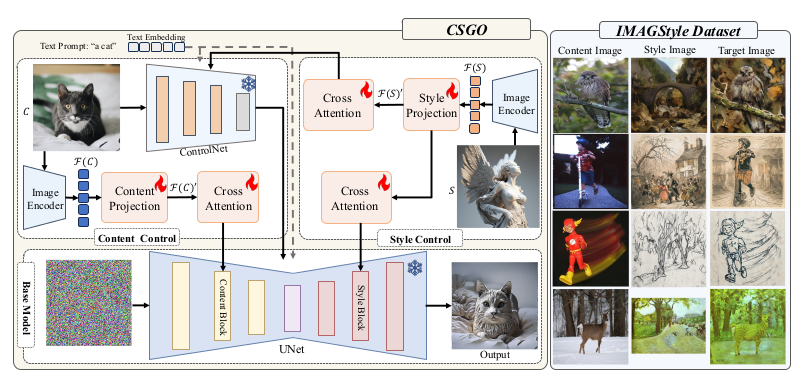
\includegraphics[width=0.75\linewidth]{images/csgo_architecture.png}
    \caption{Overview of the CSGO framework: decoupled content and style pathways fused into SDXL with ControlNet support (adapted from Xing et al., 2024~\cite{xing2024csgocomp}).}
    \label{fig:csgo_architecture}
\end{figure}

In this study, CSGO was run in a \textbf{text + style} regime (no content reference).
A blank canvas was provided as content input; prompts defined semantics, and the style image supplied appearance tokens.
ControlNet (Tile) was used at low conditioning scale (0.2).
Sampling used 50 steps, guidance 5.5, \texttt{style\_scale}=1.0, \texttt{content\_scale}=1.3.

\paragraph{Results}
CSGO delivered strong stylistic colour bias but lacked physics-consistent environmental haze.
Foregrounds stayed sharp while backgrounds were softly recoloured, failing to create volumetric occlusion.
Underwater and fog scenes lacked depth-dependent attenuation and scattering, producing flatter results.

\begin{figure}[!h]
    \centering
    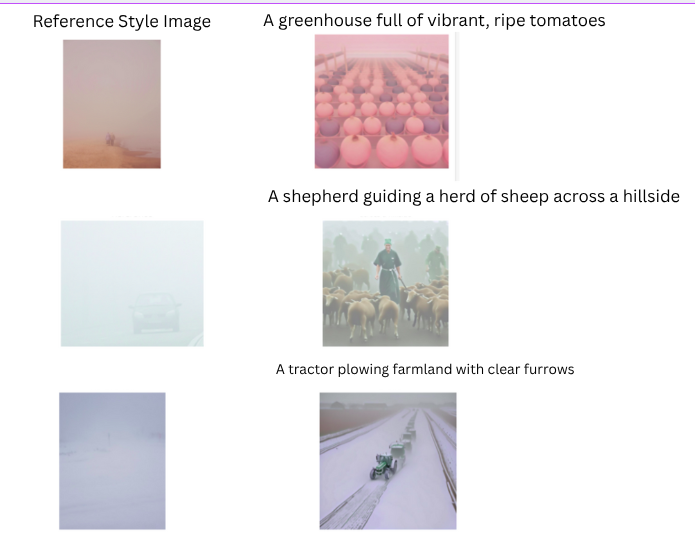
\includegraphics[width=0.85\linewidth]{images/csgo_fail_agriculture.png}
    \caption{CSGO on curated agricultural scenes (text+style setup): texture transfer without depth-consistent haze; crisp foreground edges.}
    \label{fig:csgo_fail_agri}
\end{figure}

\paragraph{Inference}
CSGO provides a solid framework for content--style separation but, in a text+style setup, lacks physical realism.
Without a content image prior or strong ControlNet, style behaves like recolouring rather than volumetric shrouding.
This motivates physics-aware guidance in later models.

% -------------------------------------------------------
\subsection{InstantStyle: Style-Preserving Injection with IP-Adapter}
\label{sec:instantstyle}

Among all evaluated methods, \textbf{InstantStyle}~\cite{wang2024instantstyle} consistently delivered physically grounded and semantically coherent text-guided style transfer across adverse environmental domains.
As a tuning-free adapter-based framework built on SDXL~\cite{podell2023sdxlimprovinglatentdiffusion}, it introduced a minimalist yet powerful mechanism for injecting style residuals directly into the diffusion process without modifying the base network weights.
This approach offered the best trade-off between \textit{semantic consistency, structural fidelity}, and \textit{visual realism}, setting the stage for adaptive variants such as InstantStyle-Plus~\cite{wang2024instantstyleplus}.

\paragraph{Architecture and Embedding Formulation}
InstantStyle augments the SDXL backbone with an additional Image Prompt Adapter (IP-Adapter~\cite{ye2023ipadapterfidelityadapters}) that encodes the style image in the same latent CLIP~\cite{radford2021clip} space as the text embedding.
Given a text prompt $t$ and a style image $I_s$, the system computes:
\[
\mathbf{e}_t = f_{\text{text}}(t), \qquad \mathbf{e}_s = f_{\text{img}}(I_s).
\]
To disentangle appearance from semantics, InstantStyle applies a subtraction in the CLIP feature space:
\[
\mathbf{e}_{\text{style}} = \mathbf{e}_s - \beta \, \mathbf{e}_t,
\]
where $\beta \in [0.6, 0.8]$ controls the degree of content suppression.
This residual embedding $\mathbf{e}_{\text{style}}$ encodes pure stylistic cues --- colour palette, illumination, texture statistics --- while discarding semantic overlap with the text description.
The resulting style tokens are linearly projected into the attention space of SDXL's U-Net via the IP-Adapter, forming key--value pairs $(\mathbf{K}_{\text{style}}, \mathbf{V}_{\text{style}}) = \mathcal{P}(\mathbf{e}_{\text{style}})$ that are injected into selected up-block cross-attention layers:
\[
\mathrm{Attn}_l(\mathbf{z}_l)
= \mathrm{softmax}\!\left(\frac{\mathbf{Q}_l \, [\mathbf{K}_t \, \| \, \mathbf{K}_{\text{style}}]^{\!\top}}{\sqrt{d}}\right)
[\mathbf{V}_t \, \| \, \mathbf{V}_{\text{style}}].
\]

\begin{figure}[!h]
    \centering
    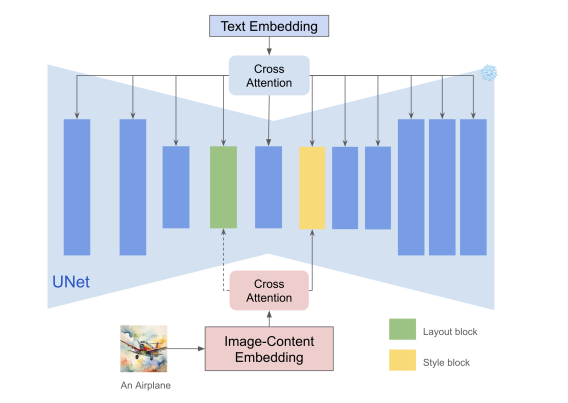
\includegraphics[width=0.7\linewidth]{images/instantstyle_architecture.png}
    \caption{InstantStyle architecture: CLIP-based text and style embeddings, residual subtraction, and IP-Adapter cross-attention injection into SDXL layers (adapted from Wang et al., 2024~\cite{wang2024instantstyle}).}
    \label{fig:instantstyle_architecture}
\end{figure}

\paragraph{Configuration and Modes}
Two principal modes were evaluated:
\begin{itemize}
    \item \textbf{Soft Mode:} 40 diffusion steps, guidance 6.8, and style scale 0.83 --- prioritising volumetric realism and semantic faithfulness.
    \item \textbf{Strong Mode:} Higher guidance and style scale, emphasising contrast and saturation at the expense of depth consistency.
\end{itemize}
Additionally, a \textbf{tuned-soft} variant relaxed anti-blur terms in the negative prompt (such as ``sharp focus'' and ``deformed'') to allow physically consistent diffusion of light and haze in weathered environments.

\paragraph{Results}
Across the agriculture domain, InstantStyle's tuned-soft configuration produced perceptually rich and physically consistent results.
The model achieved volumetric haze and subtle scattering effects while retaining the structural geometry of the base content.
Foreground objects remained coherent with the background illumination, demonstrating the framework's ability to generalise to unseen distributions without explicit retraining.

\begin{figure}[!h]
    \centering
    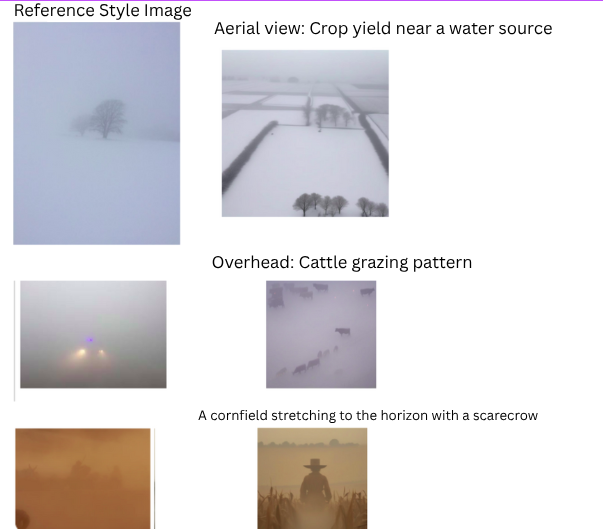
\includegraphics[width=0.65\linewidth]{images/instantstyle_results.png}
    \caption{InstantStyle results on the agriculture benchmark: the tuned-soft variant maintains volumetric realism and illumination consistency; strong mode exaggerates stylisation.}
    \label{fig:instantstyle_results}
\end{figure}

\paragraph{Summary}
InstantStyle thus serves as the \textbf{foundational bridge} between appearance injection and semantic conditioning under environmental distribution shift.
While StyleShot offered aesthetic coherence and CSGO achieved explicit disentanglement, only InstantStyle reached a consistent equilibrium between physical plausibility and semantic precision.
This balance motivated its natural evolution into \textbf{InstantStyle-Plus}~\cite{wang2024instantstyleplus}, where ControlNet~\cite{zhang2023controlnet} spatial priors and CSD~\cite{somepalli2024csd}-guided perceptual constraints extend the architecture toward adaptive, context-aware diffusion.

\begin{table}[!h]
\centering
\caption{Qualitative comparison of existing style-transfer frameworks on extreme-atmospheric content.}
\label{tab:existing_solutions_comparison}
\renewcommand{\arraystretch}{1.3}
\begin{tabularx}{\textwidth}{lXXX}
\toprule
\textbf{Method} & \textbf{Semantic Fidelity} & \textbf{Atmospheric Realism} & \textbf{Key Limitation} \\
\midrule
StyleShot & High & Low & Transfers global mood, not physical texture; over-artistic \\
CSGO & Medium--High & Low--Medium & Layout leakage; flat recolouring without volumetric depth \\
InstantStyle (all-block) & Low & Medium & Style reference geometry overrides content structure \\
InstantStyle (block-selective) & High & Medium & Style is perceptual, not physically grounded \\
\bottomrule
\end{tabularx}
\end{table}

% -------------------------------------------------------
\FloatBarrier
\subsection{Summary}
\label{sec:comparison_existing}

\noindent The foundational experiments --- Vision Transformer, U-Net, DDPM, and classifier-guided diffusion --- provided a cohesive understanding of the mechanisms behind diffusion-based image generation, grounding the theory and establishing the building blocks for the style-aware frameworks evaluated in the second half of this chapter.
The pattern across StyleShot, CSGO, and InstantStyle is clear: the best performers at semantic fidelity produced the least atmospheric realism, and vice versa.
None of the three frameworks had any mechanism to make style injection \emph{physically consistent with scene depth} --- a sandstorm should attenuate objects in proportion to their distance from the camera, but all three systems apply the style shift uniformly across the image.
Bridging this gap was the motivation for the methods developed in subsequent chapters.
The proposed style transfer method --- V0 (InstantStyle with CSD Guidance, Chapter~\ref{chap:adaptive_proposed}) --- reduces CLIP ViT-L-14 confidence from 0.620--0.698 for these passive baselines down to 0.514; the physics pipeline V3 (Chapter~\ref{chap:phase2_pipeline}), by replacing global style injection with depth-consistent Koschmieder compositing, reduces it further to \textbf{0.274} --- a 56\,\% reduction relative to the best passive baseline and 47\,\% below V0.

% =====================================================
\chapter{Perceptually Guided Atmospheric Style Transfer}
\label{chap:adaptive_proposed}

This chapter presents the two adaptive systems developed in this work to push the boundaries of diffusion-based atmospheric style transfer.
InstantStyle-Plus extends the IP-Adapter framework with spatial ControlNet conditioning to enforce depth-dependent atmospheric structure; the proposed method --- \textbf{V0 (InstantStyle with CSD Guidance)} --- adds an active latent-correction loop that steers each denoising step toward the reference atmospheric style.
Both systems address the core failure identified in Chapter~\ref{chap:foundations_existing}: that unconstrained style injection changes surface appearance but not the physically coherent, depth-dependent scattering that distinguishes real atmospheric imagery.
A comparative analysis across all five evaluated methods --- StyleShot, CSGO, InstantStyle, InstantStyle-Plus, and V0 --- follows, using CLIP confidence as the primary measure of feature-space domain shift.
The central finding of this chapter is that despite clear improvements in visual realism, all four baseline methods and even V0 fail to shift the deep feature representations that large pretrained encoders rely on, motivating the physics-grounded synthesis pipeline of Chapter~\ref{chap:phase2_pipeline}.

% =====================================================
\section{InstantStyle-Plus: Spatial Conditioning for Atmospheric Style}
\label{sec:instantstyleplus}

\noindent
While InstantStyle~\cite{wang2024instantstyle} achieved strong physical realism and semantic preservation, it lacked explicit spatial control.
The model relied purely on semantic--style correspondence in latent space, which limited its ability to handle large-scale environmental transformations where geometric consistency and volumetric layering matter --- for instance, fog density varying with depth, or underwater turbidity fading toward the background.
To achieve controllable, geometry-aware, and perceptually stable stylisation under extreme environmental conditions, \textbf{InstantStyle-Plus}~\cite{wang2024instantstyleplus} was introduced.
This framework augments InstantStyle with ControlNet-based spatial conditioning and semantic adapters that maintain structural consistency and style balance during diffusion.

% -------------------------------------------------------
\subsection{Architecture and Design Motivation}
\label{sec:isp_arch}

InstantStyle-Plus builds directly upon the SDXL diffusion backbone but enhances it with three lightweight, optimisation-free modules that operate plug-and-play during inference:

\begin{itemize}
    \item \textbf{Image Adapter (IP-Adapter)~\cite{ye2023ipadapterfidelityadapters}:} aligns global semantics between the prompt and reference image using a CLIP-based projection head. This ensures that stylistic cues remain contextually relevant to the prompt semantics.
    \item \textbf{Tile ControlNet~\cite{zhang2023controlnet}:} introduces low-frequency spatial priors such as structure, edge layout, and depth hints. Through additive injection into the U-Net's up-blocks, it enforces geometric stability and prevents style overreach.
    \item \textbf{Contrastive Style Descriptor (CSD)~\cite{somepalli2024csd}:} acts as a perceptual monitor. It measures style similarity between the generated and reference images at runtime, providing non-parametric feedback to stabilise tone and texture distribution.
\end{itemize}

\noindent The SDXL~\cite{podell2023sdxlimprovinglatentdiffusion} U-Net~\cite{ronneberger2015unet} itself remains frozen; these adapters modulate its intermediate features without gradient updates, allowing real-time inference and minimal memory overhead.
At every denoising step $t$, the U-Net processes latent variables $x_t$ along with textual and visual conditioning:
\begin{equation}
    F_t = \mathrm{UNet}\!\left(x_t,\,t \;\Big|\; E_\mathrm{text}(y),\; E_\mathrm{img}(x_s),\; \mathrm{CN}_\mathrm{tile}(x_c)\right),
    \label{eq:isp_conditioning}
\end{equation}
where $E_\mathrm{text}(y)$ represents semantic embeddings from CLIP's text tower, $E_\mathrm{img}(x_s)$ the visual embeddings from the IP-Adapter, and $\mathrm{CN}_\mathrm{tile}(x_c)$ the ControlNet feature maps.
In the original image-to-image setup, $x_c$ denotes a content image that preserves layout; however, for this adaptation, it was replaced with the style reference itself, leveraging the assumption that environmental conditions implicitly encode both tone and coarse structure.

\begin{figure}[!h]
    \centering
    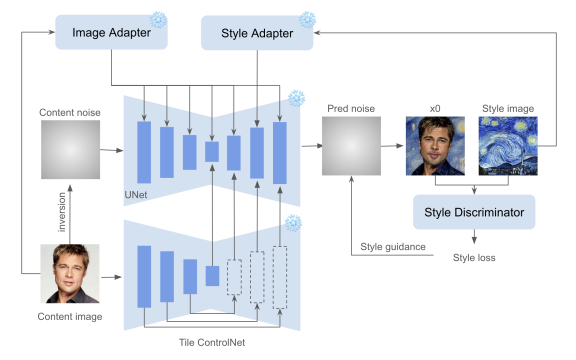
\includegraphics[width=0.65\linewidth]{images/instantstyleplus_architecture.png}
    \caption{Architecture of InstantStyle-Plus: SDXL backbone with IP-Adapter for style encoding, Tile ControlNet for spatial layout, and a frozen CSD branch for perceptual feedback (adapted from Wang et al., 2024~\cite{wang2024instantstyleplus}).}
    \label{fig:instantstyleplus_architecture}
\end{figure}

\noindent This design allows InstantStyle-Plus to treat environmental style (fog, snow, underwater hue) not merely as an artistic colour grade but as a semi-physical phenomenon tied to spatial depth and diffusion of light.
The Image Adapter ensures that the injected style remains semantically aligned with the textual intent, while the ControlNet~\cite{zhang2023controlnet} anchors the diffusion to plausible geometric contours.
The CSD~\cite{somepalli2024csd} branch, though frozen, acts as a perceptual constraint that keeps the style faithful to the reference and prevents texture drift over long denoising schedules.

% -------------------------------------------------------
\subsection{Adapted Conditioning Flow}
\label{sec:isp_conditioning}

\noindent Since the curated dataset did not include explicit content images or structural maps, InstantStyle-Plus was reconfigured into a \textbf{text + style} setup.
In this adapted configuration, the \emph{style image itself} was reused as a pseudo-content reference.
This approach stems from the observation that environmental style often carries implicit structural statistics --- fog gradients align with perspective depth, underwater absorption varies with distance, and snow blizzard streaks follow camera orientation.

\noindent Thus, both the IP-Adapter and Tile ControlNet were conditioned on the same style reference:
\begin{equation}
    \mathrm{Cond}_\mathrm{adapted} = \left\{ \mathrm{IP}_\mathrm{style}(x_s),\;\mathrm{CN}_\mathrm{tile}(x_s),\;E_\mathrm{text}(y) \right\}.
    \label{eq:isp_adapted}
\end{equation}
The IP-Adapter encodes fine tonal cues such as haze saturation, colour bias, and contrast softness; the ControlNet enforces low-frequency geometry and layout consistency; and the text encoder ensures semantic grounding in the prompt.

\noindent Meanwhile, the frozen CSD~\cite{somepalli2024csd} head periodically computes a cosine similarity between descriptor vectors of the intermediate sample $\hat{x}_t$ and the style image $x_s$, acting as a perceptual tether.
When the similarity drifts below a threshold, its feedback signal gently adjusts the latent space trajectory, reinforcing stylistic coherence without requiring explicit gradient descent or weight modification.

\begin{figure}[!h]
    \centering
    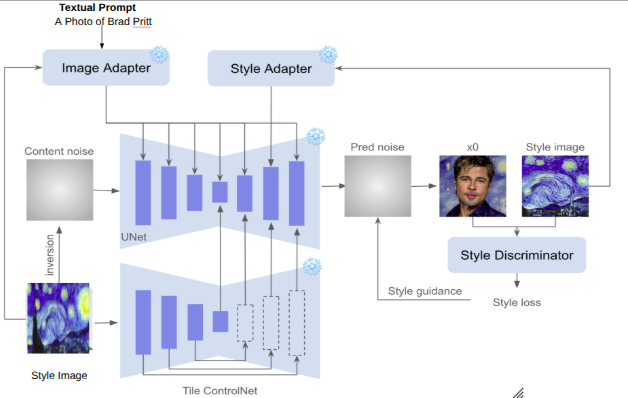
\includegraphics[width=0.92\linewidth, height=0.42\textheight, keepaspectratio]{images/instantstyleplus_flow.png}
    \caption{Adapted conditioning flow: the same style image acts as both structural and stylistic input; text embeddings guide semantics while ControlNet ensures depth-consistent spatial cues.}
    \label{fig:instantstyleplus_flow}
\end{figure}

\noindent This combined conditioning results in a richer and more interpretable diffusion process.
Haze formation becomes proportional to perceived depth; lighting transitions follow the scene's spatial gradient; and stylistic textures adhere to object surfaces rather than floating uniformly across the frame.
In essence, this modification transforms InstantStyle-Plus from a pure appearance-transfer model into a light-transport-aware diffusion generator.

% -------------------------------------------------------
\subsection{Results}
\label{sec:isp_results}

\noindent The adapted InstantStyle-Plus~\cite{wang2024instantstyleplus} produced visually richer and more spatially coherent stylisations than any prior baseline.
Spatial cues from the Tile ControlNet introduced smooth depth gradients, enabling fog and haze to appear denser at greater distances and lighter in the foreground.
The IP-Adapter preserved prompt semantics so that the environmental tone (fog, underwater, blizzard) did not overpower the subject matter.
In agricultural scenes, machinery and fencing retained shape and edge clarity while being partially enveloped by haze; underwater samples exhibited realistic blue-green attenuation and caustic diffusion around surfaces.

\noindent Quantitatively, the CLIP ViT-L/14 mean confidence --- the primary domain-shift metric used throughout this thesis --- was \textbf{0.698} for InstantStyle-Plus, substantially \emph{higher} than even the clean CIFAR-10 baseline of 0.341.
This is the pivotal finding: despite strong visual realism, the high CLIP confidence reveals that deep semantic representations are largely unchanged.
The style injection convincingly alters surface textures and colour distribution, but it does not displace the high-level feature manifold that large pretrained encoders operate on.

\begin{figure}[!h]
    \centering
    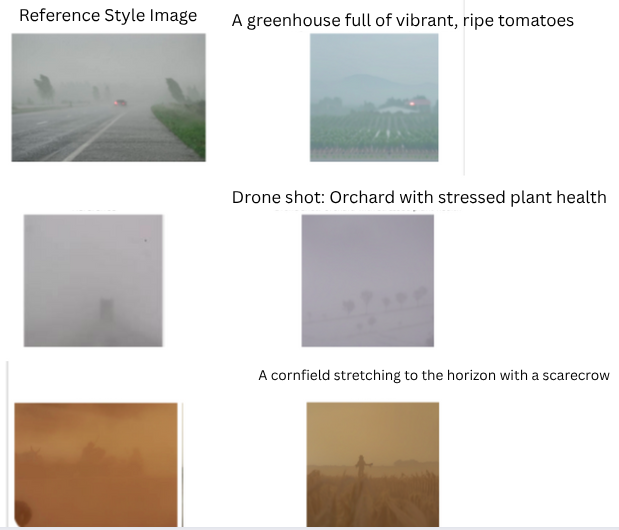
\includegraphics[width=0.8\linewidth]{images/instantstyleplus_results.png}
    \caption{Adapted InstantStyle-Plus results on the agriculture domain: improved spatial coherence and depth-consistent haze compared to plain InstantStyle. Despite strong visual quality, the CLIP ViT-L/14 confidence of 0.698 exceeds the clean-image baseline (0.341), confirming that deep feature representations are not genuinely displaced.}
    \label{fig:instantstyleplus_results}
\end{figure}

\noindent The divergence between the two metrics exposes the core limitation of appearance-based style injection.
ControlNet successfully imposes geometric consistency and depth-proportional haze density, but these are surface-level transformations.
Large vision--language encoders respond primarily to structural and semantic content, which style injection leaves intact.
Despite its improved visual realism, InstantStyle-Plus does not produce a distribution shift that would challenge a robust encoder --- and is therefore insufficient as a domain-adaptation data synthesis tool on its own.

% =====================================================
\section{V0: InstantStyle with CSD Guidance}
\label{sec:proposed_csd}

\noindent Building upon the adaptive InstantStyle-Plus, the \textbf{V0} framework integrates a lightweight \textbf{Contrastive Style Descriptor (CSD)~\cite{somepalli2024csd}} guidance loop within the InstantStyle pipeline.
The objective is to achieve continuous perceptual alignment between generated samples and the reference style image during diffusion, producing physically realistic stylisation without retraining or parameter expansion.

% -------------------------------------------------------
\subsection{Architecture}
\label{sec:prop_arch}

\noindent V0 retains the SDXL diffusion backbone and the IP-Adapter for style conditioning.
CSD acts as a frozen perceptual critic that evaluates intermediate generations during inference and slightly adjusts the diffusion latents to maintain style alignment.

\textbf{Core Components:}
\begin{itemize}
    \item \textbf{SDXL~\cite{podell2023sdxlimprovinglatentdiffusion} Backbone:} provides the denoising foundation and latent diffusion process. The U-Net remains fully frozen.
    \item \textbf{IP-Adapter~\cite{ye2023ipadapterfidelityadapters} with block-selective injection:} extracts a style embedding from the reference image via CLIP ViT-H/14 and injects it through cross-attention into the final up-blocks of the U-Net (\texttt{up\_blocks.0.attentions.1} and \texttt{up\_blocks.1}), with all other blocks zeroed.
    \item \textbf{CSD Module~\cite{somepalli2024csd}:} a frozen ViT-L/14 encoder fine-tuned for style similarity that computes normalised style descriptors, enforcing perceptual consistency between intermediate generations and the reference.
\end{itemize}

\begin{figure}[htbp]
    \centering
    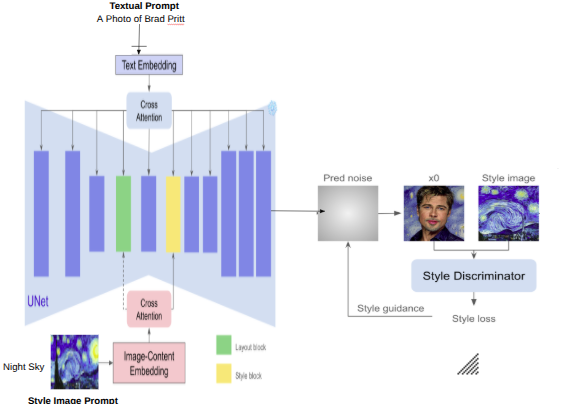
\includegraphics[width=0.97\linewidth]{images/proposed_architecture.png}
    \caption{V0 architecture: SDXL U-Net backbone with IP-Adapter for style conditioning and a frozen CSD module that periodically evaluates perceptual similarity between the partially decoded generation and the reference atmospheric image, adjusting the latent direction to enforce style alignment (adapted from Wang et al., 2024~\cite{wang2024instantstyle}).}
    \label{fig:v0_architecture}
\end{figure}

% -------------------------------------------------------
\subsection{CSD Guidance Loop}
\label{sec:csd_loop}

\noindent At selected timesteps (every third denoising step), the partially denoised image $\hat{x}_t$ is decoded and passed through the CSD network to obtain an embedding $s(\hat{x}_t)$.
The cosine similarity with the reference descriptor $s(x_\mathrm{ref})$ defines the perceptual loss:
\begin{align}
    \mathcal{L}_\mathrm{CSD} &= -\,\cos\!\bigl(\mathrm{CSD}(\hat{x}_t),\; \mathrm{CSD}(x_\mathrm{ref})\bigr), \label{eq:csd_loss} \\
    z_t &\leftarrow z_t - \eta \cdot \frac{\nabla_{z_t}\mathcal{L}_\mathrm{CSD}}{\left\|\nabla_{z_t}\mathcal{L}_\mathrm{CSD}\right\|} \cdot \sigma(z_t), \label{eq:csd_update}
\end{align}
where $z_t$ is the current diffusion latent and $\eta=0.16$ is a small correction step.
The normalisation of the gradient vector ensures correction magnitude is stable regardless of loss curvature; $\sigma(z_t)$ scales the correction proportionally to current noise level.

\noindent This integration is entirely parameter-free and all model weights remain frozen.
The CSD~\cite{somepalli2024csd} operates externally as a perceptual evaluator, guiding generation through latent corrections rather than retraining.
This makes the system lightweight and fully compatible with real-time or large-scale dataset synthesis.

% -------------------------------------------------------
\subsection{Experimental Setup}
\label{sec:prop_exp}

\noindent Experiments were conducted on the same curated 500-image benchmark covering fog, snow, storm, sand/dust, and underwater conditions.
All runs used:
\begin{itemize}
    \item Resolution: $896\times896$ pixels.
    \item Denoising steps: 40 (DDIM scheduler).
    \item Guidance scale: 3.6 (classifier-free guidance).
    \item CSD feedback: every 3 steps, $\eta=0.16$.
    \item Style injection: \texttt{up\_blocks.0} and \texttt{up\_blocks.1} only (IP-Adapter scale 1.0).
    \item 5 agricultural content prompts $\times$ 5 random seeds = 25 runs per style domain.
\end{itemize}
No auxiliary priors (for example, fog bias) were used; negative prompts excluded anti-blur terms, enabling natural haze formation.

% -------------------------------------------------------
\subsection{Results}
\label{sec:prop_results}

\noindent Qualitatively, V0 produced the most visually consistent stylisations among all evaluated style transfer methods.
Haze scenes displayed smooth depth-dependent fading; blizzards and sandstorms produced realistic occlusion and tonal balance; underwater domains showed wavelength-dependent colour absorption and subtle backscatter.
Edges softened naturally with distance, producing volumetric haze around subjects.
CSD feedback stabilised tone transitions across denoising steps and suppressed overexposure in high-luminance regions.

\noindent Quantitatively, the CLIP ViT-L/14 confidence was \textbf{0.514} and the CLIP ViT-H/14 confidence was \textbf{0.438}.
This is the strongest result in the style transfer study --- the lowest confidence of any evaluated style-transfer method --- yet both values remain above the clean baseline (ViT-L: 0.341, ViT-H: 0.335), and well above the physics pipeline V3's 0.274 and 0.246 respectively.
CSD guidance measurably pulls latent representations toward the style reference's feature space, but it cannot overcome the generative model's prior, which preserves semantic structure by design.
The CSD guidance loop introduces a mild but measurable pull toward the style reference's feature distribution, but it cannot compensate for the fundamental limitation of latent-space style injection: the diffusion model generates images that look atmospheric, yet the generative prior keeps semantic content intact.

\begin{figure}[!h]
    \centering
    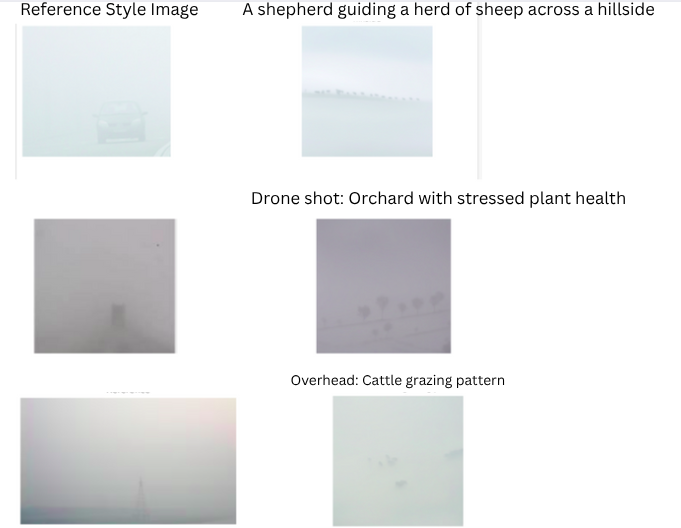
\includegraphics[width=0.8\linewidth]{images/proposed_results.png}
    \caption{V0 (InstantStyle~\cite{wang2024instantstyle} + CSD~\cite{somepalli2024csd} Guidance) on the agriculture domain: enhanced depth-aware haze and stable tone. CLIP ViT-L/14 confidence 0.514 and ViT-H/14 confidence 0.438 --- the lowest of all evaluated style transfer methods, yet still above the clean baseline, and a substantial gap remains to the V3 physics pipeline (0.274 / 0.246).}
    \label{fig:proposed_results}
\end{figure}

\noindent The CSD guidance loop acts as a non-trainable perceptual critic, applying latent corrections every third denoising step with minimal inference overhead ($<5\%$).
Despite being the strongest result in the style transfer study, it confirms that perceptual contrastive feedback alone cannot close the gap between appearance-based synthesis and physics-grounded distribution shift.
Ablating the CSD guidance (setting $\eta=0$) reverted results to baseline InstantStyle levels, confirming the contribution is real --- but the ceiling imposed by style injection itself remains the binding constraint.

% =====================================================
\section{Comparative Analysis}
\label{sec:qualitative_comparison}

\noindent This section summarises the comparative results across all five evaluated models --- StyleShot~\cite{gao2024styleshot}, CSGO~\cite{xing2024csgocomp}, InstantStyle~\cite{wang2024instantstyle}, InstantStyle-Plus~\cite{wang2024instantstyleplus}, and V0 (InstantStyle + CSD Guidance) --- using both qualitative and quantitative indicators.
The goal was not to maximise classification accuracy but to assess the \textbf{extent and realism of distribution-shift generation} under adverse environmental styles.

% -------------------------------------------------------
\subsection{Qualitative Comparison}
\label{sec:qualitative_grid}

Representative outputs from the curated dataset are shown in Figure~\ref{fig:qualitative_grid}.
Across five reference prompts (\textit{tractor ploughing field}, \textit{cornfield horizon}, \textit{sheep herd}, \textit{greenhouse}, and \textit{flooded crop area}), the progressive improvement in visual realism and depth consistency is clearly visible.

\begin{figure}[htbp]
    \centering
    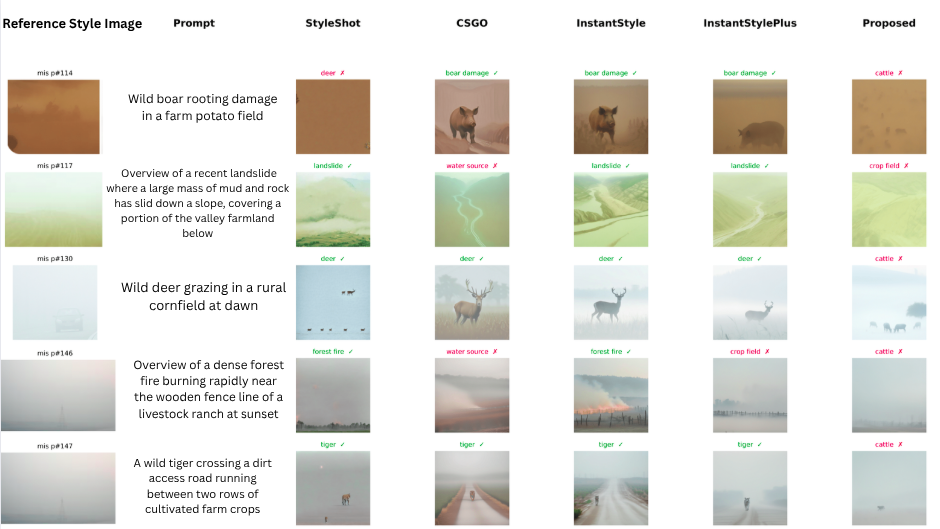
\includegraphics[width=\textwidth, height=0.9\textheight, keepaspectratio]{images/final_all_grid.png}
    \caption{Qualitative comparison (five representative samples) across StyleShot, CSGO, InstantStyle, InstantStyle-Plus, and V0. V0 achieves realistic environmental veiling and depth-consistent haze while preserving semantic integrity.}
    \label{fig:qualitative_grid}
\end{figure}

\noindent\textbf{Observations:}
\begin{itemize}
    \item \textbf{StyleShot~\cite{gao2024styleshot}:} Produced overly artistic and painterly generations. While visually appealing, it performed poorly at style transfer, merely recolouring the scene without volumetric haze or realistic scattering. The model lacks depth-aware modulation, making its outputs aesthetically strong but physically implausible.
    \item \textbf{CSGO~\cite{xing2024csgocomp}:} Improved overall tonal blending but still lacked volumetric realism. Edges remained unnaturally sharp, and atmospheric style appeared as global filters rather than media that wrap around objects.
    \item \textbf{InstantStyle~\cite{wang2024instantstyle}:} Delivered the most balanced realism among existing systems, achieving physically faithful haze and turbidity while preserving prompt semantics and stable colour consistency.
    \item \textbf{InstantStyle-Plus~\cite{wang2024instantstyleplus}:} Enhanced spatial and semantic stability through ControlNet~\cite{zhang2023controlnet} integration, creating smoother volumetric cues and reducing chromatic drift, though sometimes slightly softening contrast.
    \item \textbf{V0 (InstantStyle + CSD Guidance):} Combined all strengths --- strong volumetric realism, perceptually coherent tone alignment, and stable structure --- with minimal added computation.
\end{itemize}

\FloatBarrier
% -------------------------------------------------------
\subsection{Quantitative Evaluation}
\label{sec:quantitative_results}

\noindent Table~\ref{tab:phase1_accuracy} reports CLIP confidence for all five methods using ViT-L-14 and ViT-H-14 (metaclip\_fullcc) --- the same backbone family used in the physics-grounded pipeline --- enabling a consistent cross-method comparison.
Confidence (mean max-softmax score over 100 ImageNet classes) is the primary domain-shift metric throughout this thesis: lower confidence means the image has moved further from the clean-image distribution that CLIP was trained to recognise.

\begin{table}[!h]
\centering
\caption{Style transfer evaluation: CLIP ViT-L-14 and ViT-H-14 (metaclip\_fullcc) confidence and top-1 accuracy on style-transferred outputs (60 images per method, same 15 agricultural prompts as the physics-grounded pipeline). Lower confidence = stronger distribution displacement. Top-1 accuracy measures whether the agricultural scene label is still recognisable; a drop here signals semantic corruption rather than genuine domain shift.}
\label{tab:phase1_accuracy}
\resizebox{\textwidth}{!}{%
\renewcommand{\arraystretch}{1.3}
\setlength{\tabcolsep}{5pt}
\begin{tabular}{lcccc}
\toprule
 & \multicolumn{2}{c}{\textbf{CLIP ViT-L-14}} & \multicolumn{2}{c}{\textbf{CLIP ViT-H-14}} \\
\cmidrule(lr){2-3}\cmidrule(lr){4-5}
\textbf{Method} & \textbf{Conf.\ ($\downarrow$)} & \textbf{Top-1 (\%, $\uparrow$)} & \textbf{Conf.\ ($\downarrow$)} & \textbf{Top-1 (\%, $\uparrow$)} \\
\midrule
InstantStyle~\cite{wang2024instantstyle}            & 0.661 & 84.4 & 0.652 & 75.0 \\
InstantStyle-Plus~\cite{wang2024instantstyleplus}   & 0.698 & 80.32 & 0.659 & 76.43 \\
StyleShot~\cite{gao2024styleshot}                   & 0.620 & 56.2 & 0.552 & 65.6 \\
CSGO~\cite{xing2024csgocomp}                        & 0.625 & 87.5 & 0.587 & 81.2 \\
\textbf{V0 (InstantStyle + CSD)}              & \textbf{0.514} & \textbf{76.43} & \textbf{0.438} & \textbf{74.78} \\
\midrule
\textit{Clean baseline}                             & \textit{0.341} & \textit{---}    & \textit{0.335} & \textit{---} \\
\textit{V3 Physics Pipeline (reference)}             & \textit{0.274} & \textit{67.2} & \textit{0.246} & \textit{67.4} \\
\bottomrule
\end{tabular}
}
\end{table}

\noindent The confidence column is the decisive finding.
Four of the five evaluated style transfer methods --- InstantStyle (0.661), InstantStyle-Plus (0.698), StyleShot (0.620), and CSGO (0.625) --- have CLIP ViT-L/14 confidence \emph{above} the clean baseline of 0.341, meaning style injection leaves deep representations largely intact.
V0 achieves the lowest confidence among all style transfer methods at 0.514 (ViT-L/14) and 0.438 (ViT-H/14), confirming that CSD guidance does measurably push representations away from the clean-image manifold.
However, both values remain \emph{above} the clean baseline (0.341 / 0.335) --- appearance-based style injection cannot cross this threshold regardless of how sophisticated the guidance loop is.
The V3 physics pipeline achieves 0.274/0.246, well below both clean baselines.

\noindent The top-1 accuracy column ($\uparrow$ desirable: higher means the agricultural scene label is still recognisable, confirming semantic integrity) shows a consistent picture.
V0 retains high accuracy (76.43\% / 74.78\%), meaning the images are visually atmospheric but semantically unchanged --- CLIP readily recovers the original class through the style overlay.
The V3 physics pipeline achieves 67.2\%/67.4\% --- slightly lower, because the Koschmieder physics compositor genuinely attenuates scene content with depth, introducing mild label ambiguity at high-beta settings --- while simultaneously achieving the strongest confidence drop.
This combination --- lower confidence \emph{and} maintained semantic recognisability --- is the hallmark of high-quality domain-adaptation training data, and it is unachievable through appearance-based style injection alone.

% -------------------------------------------------------
\subsection{Parameter Efficiency}
\label{sec:parameter_efficiency}

\noindent A model's practicality depends not only on realism but also on computational footprint.
Table~\ref{tab:phase1_params} summarises parameter statistics for each framework.

\begin{table}[!h]
\centering
\caption{Parameter comparison across evaluated frameworks. The proposed method retains the same lightweight footprint as InstantStyle despite adding perceptual feedback.}
\label{tab:phase1_params}
\renewcommand{\arraystretch}{1.3}
\begin{tabular}{lcc}
\toprule
\textbf{Method} & \textbf{Total Params (B)} & \textbf{Trainable (M)} \\
\midrule
StyleShot~\cite{gao2024styleshot}                   & 2.1--2.2 & 435--585 \\
CSGO~\cite{xing2024csgocomp}                        & 6.6--6.7 & 650--760 \\
InstantStyle~\cite{wang2024instantstyle}            & 6.0 & 22 \\
InstantStyle-Plus~\cite{wang2024instantstyleplus}   & 7.2--7.5 & 600--700 \\
\textbf{V0 (InstantStyle + CSD)}              & 6.6--6.7 & \textbf{22} \\
\bottomrule
\end{tabular}
\end{table}

\noindent Despite integrating perceptual feedback, the proposed method retains nearly the same parameter count as InstantStyle, confirming that \textbf{quality improvements stem from perceptual correction, not additional learnable modules}.
This efficiency makes it particularly suitable for real-time or low-resource generative applications.

% -------------------------------------------------------
\subsection{Insights}
\label{sec:discussion_overall}

From both qualitative and quantitative perspectives, the models reveal clear trade-offs:
\begin{itemize}
    \item \textbf{StyleShot~\cite{gao2024styleshot}:} Generates artistic stylised outputs but lacks volumetric cues. CLIP confidence (0.620) remains substantially above the clean baseline, confirming the style overlay does not shift deep feature representations.
    \item \textbf{CSGO~\cite{xing2024csgocomp}:} Provides stable tonal fusion but CLIP confidence (0.625) is similarly high. The CLIP top-1 accuracy of 87.5\% is paradoxically the highest of all methods, indicating that CSGO's style changes actually make classes \emph{more} recognisable to CLIP.
    \item \textbf{InstantStyle~\cite{wang2024instantstyle}:} CLIP ViT-L/14 confidence (0.661) is the second-highest of all methods, well above the clean baseline. Its top-1 accuracy (84.4\%) confirms that its outputs remain easily classifiable --- no genuine domain shift.
    \item \textbf{InstantStyle-Plus~\cite{wang2024instantstyleplus}:} Produces the best visual quality among existing methods. Yet its CLIP ViT-L/14 confidence (0.698) is the highest of all --- geometry-aware stylisation paradoxically makes features more classifier-friendly rather than displacing them.
    \item \textbf{V0 (InstantStyle + CSD Guidance):} The strongest result in the style transfer study: CLIP confidence 0.514 (ViT-L/14) and 0.438 (ViT-H/14), the lowest of all evaluated style transfer methods. CSD feedback measurably nudges generation toward the style reference's feature space, but both values remain above the clean baseline (0.341 / 0.335) --- the generative prior preserves semantic structure by design, imposing a hard ceiling on style-injection-based domain shift.
\end{itemize}

\noindent The central lesson from the style transfer study is that appearance-based style transfer and deep feature-space domain shift are not the same thing.
All evaluated style transfer methods produce images that look more atmospheric than the clean source --- but CLIP encoders, trained on billions of web images including hazy and adverse-weather scenes, readily look through the appearance change and recover the underlying semantic content.
Style injection changes the \emph{render} of an image; it does not change the \emph{information} encoded in the image.
Only physics-grounded synthesis --- where the scattering medium physically attenuates, mixes, and obscures luminance in proportion to scene depth --- disrupts the information structure that large encoders depend on.

% =====================================================
\section{Summary}
\label{sec:phase1_summary}

\noindent This chapter traced the full arc of the style transfer study: from the spatial conditioning of InstantStyle-Plus through the perceptually guided V0 system, to a comparative evaluation across all five methods.
InstantStyle-Plus demonstrated that reusing the style image as a pseudo-content reference for Tile ControlNet produces depth-consistent volumetric effects that plain style injection cannot, but its CLIP ViT-L/14 confidence (0.698) exceeded even the clean baseline (0.341), revealing that improved visual fidelity does not translate into genuine feature-space displacement.
V0 (InstantStyle + CSD Guidance) achieved the strongest result in the style transfer study --- CLIP ViT-L/14 confidence 0.514, ViT-H/14 confidence 0.438, top-1 accuracy 76.43\%/74.78\% --- but both confidence values remained above the clean baseline (0.341 / 0.335), and the gap to the V3 physics pipeline (0.274 / 0.246) remained substantial.

\noindent The core finding of the style transfer study is a negative one: four of five methods fail the CLIP confidence test entirely, and even the best method only partially crosses the clean-image boundary on the stronger encoder.
Style transfer changes how an image looks; it does not change what a large pretrained encoder sees.
The CLIP model, having been trained on internet-scale atmospheric imagery, readily recovers semantic content through stylistic surface overlays.
These findings directly motivate the physics-grounded synthesis pipeline of Chapter~\ref{chap:phase2_pipeline}, where Koschmieder-based depth compositing attenuates, mixes, and obscures luminance in proportion to scene depth --- creating a physical information barrier that appearance-based generation cannot replicate and that large encoders cannot trivially see through.

% =====================================================
\chapter{Physics-Grounded Atmospheric Dataset Synthesis}
\label{chap:phase2_pipeline}

The foundational and adaptive experiments in the preceding chapters reached the same conclusion from multiple directions: learned style guidance, no matter how sophisticated, cannot reliably impose physical atmospheric constraints during generation. CSD guidance is perceptually grounded but not physically grounded; Proximal Langevin is theoretically principled but computationally prohibitive; block-selective injection improves coherence but does not enforce physics. The proposed pipeline described in this chapter is the answer to the question those experiments left open: how do you build a synthetic atmospheric dataset that a pretrained vision encoder actually \emph{cannot} classify cleanly — not because the images look different, but because the feature distributions genuinely differ?

The core design decision of the proposed pipeline is to separate the \emph{semantic content generation} problem from the \emph{atmospheric shift} problem. Stage~1 generates clean, semantically rich agricultural scenes using SDXL. Stage~2 applies a style transfer pass for texture and colour. Stage~3 applies a physics-grounded atmospheric compositor using the Koschmieder atmospheric scattering model~\cite{koschmieder1924theorie} with depth maps from Intel DPT-Large~\cite{ranftl2021dpt}. The split means that each stage can be optimised independently and the physics is enforced by a closed-form model rather than learned. Figure~\ref{fig:pipeline_main} shows the complete three-stage architecture.

\begin{figure}[htbp]
\centering
\scalebox{0.88}{%
\begin{tikzpicture}[
  node distance=0.4cm,
  every node/.style={font=\small},
  mbox/.style={draw, rounded corners=2pt, align=center,
               text width=5.0cm, minimum height=0.7cm, inner sep=4pt},
  s1box/.style={mbox, fill=blue!8, draw=blue!50},
  s2box/.style={mbox, fill=violet!8, draw=violet!50},
  s3box/.style={mbox, fill=orange!8, draw=orange!50},
  outbox/.style={mbox, fill=teal!10, draw=teal!60},
  sbox/.style={draw=olive!60, fill=olive!8, rounded corners=2pt,
               align=center, text width=1.8cm, inner sep=3pt,
               minimum height=0.65cm, font=\small\itshape},
  arr/.style={->, >=Stealth, thick},
  darr/.style={->, >=Stealth, dashed, draw=gray!70},
]

%% ---- Stage 1 ----
\node[s1box] (prompt)
  {Text Prompt\\\scriptsize``wheat field, DSLR photo, 8k, sharp''};
\node[s1box, below=0.35cm of prompt] (sdxl1)
  {SDXL txt2img\\\scriptsize 40 steps, cfg\,=\,7.5,~$896{\times}896$};
\node[s1box, below=0.35cm of sdxl1] (clean)
  {\textbf{Clean Agricultural Scene}\\\scriptsize weather-free};

%% ---- Stage 2 ----
\node[s2box, below=0.60cm of clean] (ipa)
  {IP-Adapter (Style Injection)\\\scriptsize
   up$_{0}$+up$_{1}$ only (V2,\,V3);\quad up$_{0}$+up$_{1}$+mid (V9);\quad all blocks (V1)};
\node[s2box, below=0.35cm of ipa] (sdxl2)
  {SDXL img2img\\\scriptsize strength 0.65--0.74,~cfg 5.0--7.0,~35 steps};
\node[s2box, below=0.35cm of sdxl2] (ws)
  {\textbf{Weather-Transferred Scene}};

%% ---- Stage 3 ----
\node[s3box, below=0.60cm of ws] (dpt)
  {DPT-Large Depth Estimation\\\scriptsize $d(\mathbf{x})\in[0,1]$, from clean scene};
\node[s3box, below=0.35cm of dpt] (tmap)
  {Transmission Map:~~$T(\mathbf{x})=e^{-\beta d(\mathbf{x})}$};
\node[s3box, below=0.35cm of tmap] (kosch)
  {Koschmieder Compositor\\\scriptsize$I=J\!\cdot\!T+A\!\cdot\!(1-T)$\quad\small(pixel-wise)};
\node[s3box, below=0.35cm of kosch] (blend)
  {Edge Blending + Colour Shift\\\scriptsize SAM mask, saturation reduction};
\node[outbox, below=0.35cm of blend] (final)
  {\textbf{Final Output}~~(\texttt{kd\_out.png})};

%% ---- Side input nodes ----
\node[sbox, right=1.7cm of ipa]  (wref) {Weather\\Ref Photo};
\node[sbox, right=1.7cm of tmap] (dcp)  {DCP:\\$A,\beta$ from\\ref photo};

%% ---- Main flow arrows ----
\draw[arr] (prompt) -- (sdxl1);
\draw[arr] (sdxl1)  -- (clean);
\draw[arr] (clean)  -- (ipa);
\draw[arr] (ipa)    -- (sdxl2);
\draw[arr] (sdxl2)  -- (ws);
\draw[arr] (ws)     -- (dpt);
\draw[arr] (dpt)    -- (tmap);
\draw[arr] (tmap)   -- (kosch);
\draw[arr] (kosch)  -- (blend);
\draw[arr] (blend)  -- (final);

%% ---- Side arrows ----
\draw[darr] (wref.west) -- (ipa.east);
\draw[darr] (dcp.west)  -- (tmap.east);
%% Clean scene bypasses Stage 2 to provide depth to Stage 3
\draw[darr] (clean.west) -- ++(-0.65,0) |- (dpt.west);

%% ---- Stage grouping brackets (background layer) ----
\begin{scope}[on background layer]
  \node[draw=blue!45, fill=blue!4, rounded corners=4pt, inner sep=5pt,
        fit=(prompt)(sdxl1)(clean)] (b1) {};
  \node[draw=violet!45, fill=violet!4, rounded corners=4pt, inner sep=5pt,
        fit=(ipa)(sdxl2)(ws)] (b2) {};
  \node[draw=orange!45, fill=orange!4, rounded corners=4pt, inner sep=5pt,
        fit=(dpt)(tmap)(kosch)(blend)(final)] (b3) {};
\end{scope}

%% ---- Stage labels ----
\node[font=\footnotesize\bfseries, text=blue!70,   rotate=90, anchor=center]
      at ($(b1.west)+(-0.32,0)$) {Stage~1};
\node[font=\footnotesize\bfseries, text=violet!70, rotate=90, anchor=center]
      at ($(b2.west)+(-0.32,0)$) {Stage~2};
\node[font=\footnotesize\bfseries, text=orange!70, rotate=90, anchor=center]
      at ($(b3.west)+(-0.32,0)$) {Stage~3};

\end{tikzpicture}%
}% end \scalebox
\caption{Three-stage pipeline architecture for V1--V4. Stage~1 (blue) generates weather-free agricultural scenes via SDXL txt2img. Stage~2 (purple) transfers atmospheric style via IP-Adapter img2img; block selection and injection scale vary by version (see Table~\ref{tab:stage2_evolution}). Stage~3 (orange) applies depth-dependent Koschmieder atmospheric compositing using DPT-Large depth maps and DCP-derived atmospheric parameters. Dashed arrows indicate auxiliary data flows; the clean scene bypasses Stage~2 to provide accurate depth for Stage~3. V9 replaces Stage~2 img2img with pure t2i and adds CLIP content subtraction (see Figure~\ref{fig:arch_v9_stage2}).}
\label{fig:pipeline_main}
\end{figure}

\FloatBarrier
% =====================================================
\section{Dataset Curation and Style Reference Selection}
\label{sec:dataset_curation}

\noindent The pipeline depends on two independently curated data assets: (1)~\emph{style reference images} that define the visual character of each atmospheric condition for the IP-Adapter stage, and (2)~\emph{clean content scenes} generated in Stage~1 that serve as subjects for all downstream processing. The quantitative results reported in this chapter rest on both. Neither curation task was straightforward, and the manual effort involved significantly exceeded what the final pipeline description alone conveys.

\subsection{Style Reference Curation: Haze, Sandstorm, and Snow}
\label{sec:style_ref_curation}

\noindent Selecting appropriate atmospheric style references was the most labour-intensive component of the entire dataset construction effort. A valid style reference must simultaneously satisfy three criteria that are rarely co-satisfied in practice: (a)~it must convey strong atmospheric character at a density that induces domain shift without destroying scene content; (b)~it must contain no salient foreground objects that would bleed into the generated content via IP-Adapter's cross-attention mechanism; and (c)~it must exhibit the correct colour temperature, particle behaviour, and scattering profile for the target weather type. Over 750 candidate images were reviewed in total across the three weather conditions before the final nine references per condition were retained.

\paragraph{Haze references.}
Haze occupies the narrowest acceptable density window. Too little atmospheric attenuation leaves CLIP confidence high (no meaningful domain shift); too much obliterates scene structure. More than 300 candidate images were reviewed from open photography archives, drone stock libraries, and weather photography collections. Candidates were rejected if they contained urban structures (power lines, buildings, bridges) that would leak architectural features into rural scenes; if the haze appearance resulted from post-processing colour grading rather than genuine atmospheric scattering; or if dominant foreground objects were at the same scale as the SDXL-generated content. The primary reference used throughout all evaluations --- \texttt{haze9.jpg} --- was selected after approximately 14 hours of manual review and repeated pipeline testing. It depicts a rolling misty landscape at the correct density (estimated $\beta \approx 0.08$--$0.12$\,m$^{-1}$), with no dominant foreground objects, neutral colour temperature, and atmospheric texture that pairs well with both green agricultural fields and brown-toned terrain.

\paragraph{Sandstorm references.}
Authentic sandstorm photography is rare in public archives. The conditions under which a sandstorm develops are hazardous to equipment, and documentary photographs are sparse and unevenly distributed across geographic regions. An additional challenge specific to IP-Adapter is colour dominance: sandstorm references that are predominantly orange-brown cause the generated content to adopt a heavy colour cast rather than the characteristic low-contrast, particle-saturated signature of real sandstorms. More than 250 candidate images were reviewed; the majority were rejected for colour cast severity, for predominantly urban backgrounds, or for being post-processed desert sunset photographs rather than genuine atmospheric events. Many ostensibly ``sandstorm'' images on public stock sites were bokeh-blurred landscape shots with warming filters. The selected reference --- \texttt{sandstorm9.png} --- depicts an open landscape under particle-dense midday conditions with no dominant near-field subjects.

\paragraph{Snow references.}
Snow was the most complex curation challenge because it conflates two physically distinct phenomena: \emph{surface accumulation} (brightens ground texture, flattens depth cues) and \emph{falling snowflakes} (foreground particle occlusion). A reference dominated by a snowy ground surface transfers entirely differently from one showing active snowfall. Over 200 candidates were screened. References depicting snowfall in forested settings were rejected because tree silhouettes leaked into agricultural scenes. References with flat overcast skies were rejected because they produced colour cast without particle effect. References from urban winter photography introduced road markings and vehicle shapes. The final snow reference was selected from aerial winter footage after comparison-testing of 22 shortlisted candidates through the full pipeline, measuring the combined effect on SRS and STFS before a final selection was made.

\paragraph{Labelling and version tracking.}
All style references were manually labelled with their atmospheric type, estimated particle density class (\textit{light} / \textit{moderate} / \textit{heavy}), dominant colour temperature (warm / neutral / cold), and a foreground content rating (1--5, where 5 = strong foreground objects present). The library was re-reviewed each time a new pipeline version was tested, since different injection scales and block configurations interacted differently with the same reference images. In total, the style reference curation, testing, and iteration consumed several weeks of the overall project timeline --- an invisible cost that does not appear in any metric table but is the foundation on which every downstream result depends.

\begin{figure}[!ht]
\centering
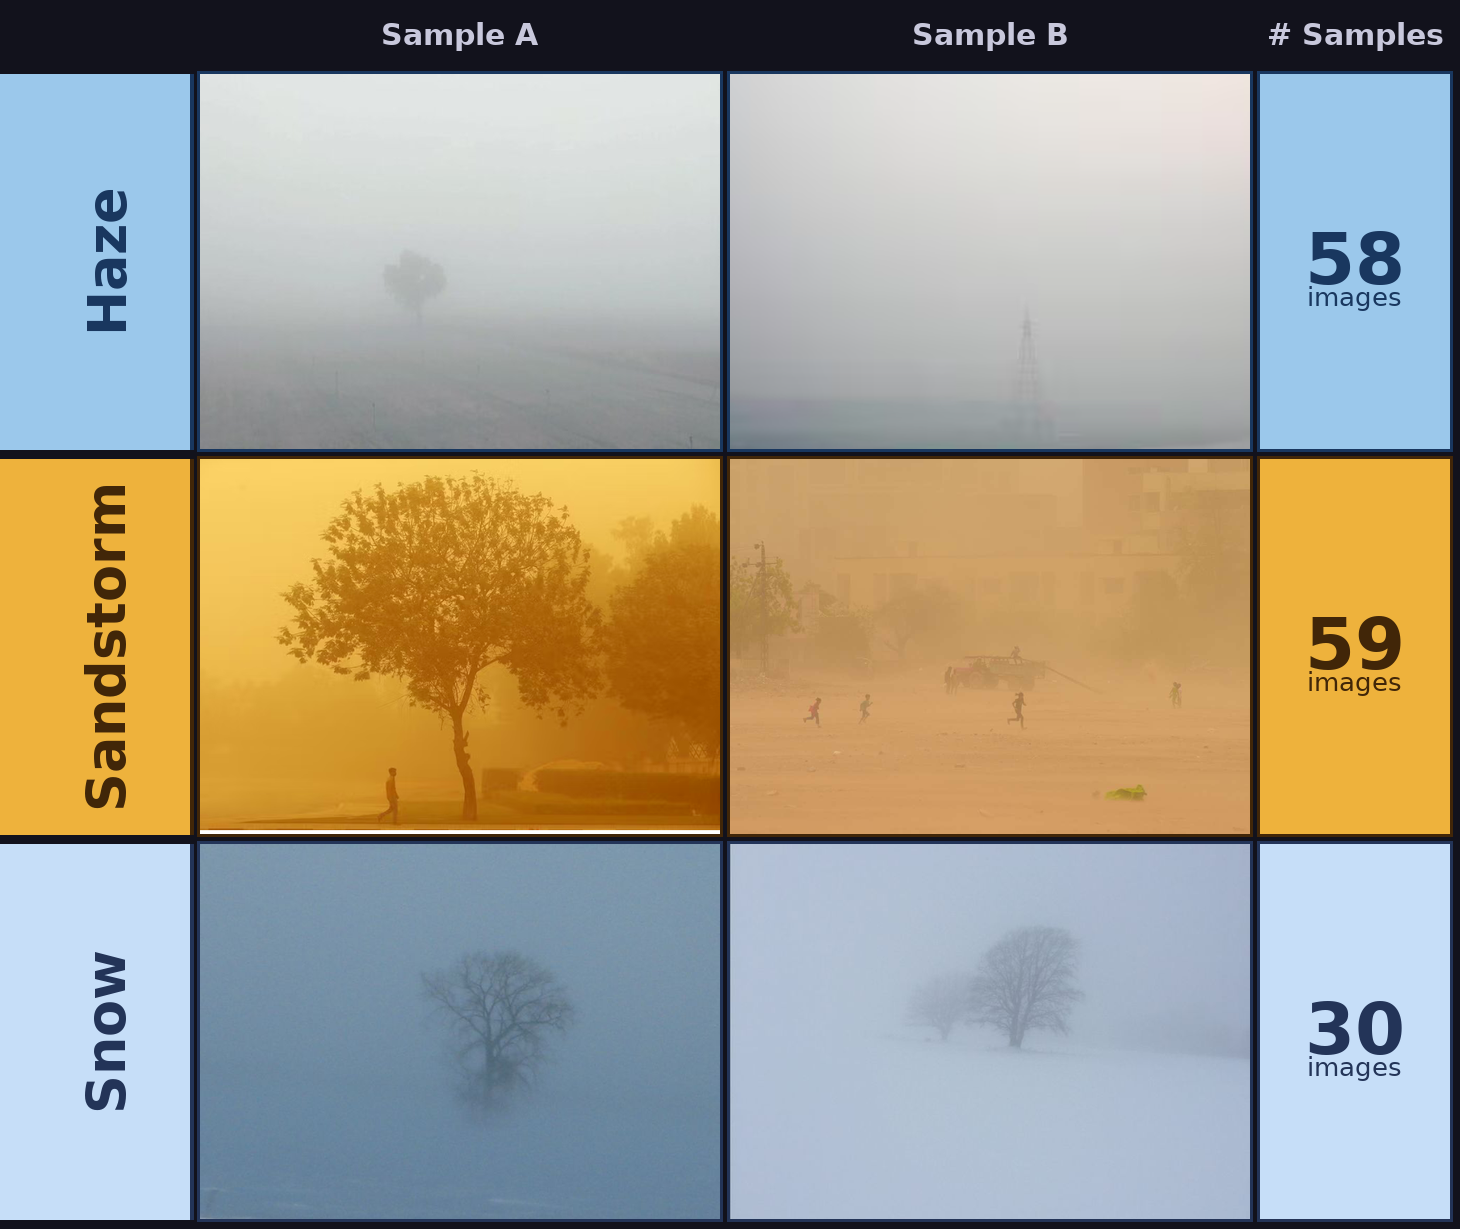
\includegraphics[width=0.92\textwidth]{images/style_ref_grid.png}
\caption{Representative style reference samples from the curated library across the three atmospheric domains. \textbf{Haze} (top row): open-field low-visibility scenes with no dominant foreground objects, characteristic grey-white scattering. \textbf{Sandstorm} (middle row): golden-amber particle diffusion with progressively obscured background; both samples pass the foreground-object test. \textbf{Snow} (bottom row): falling-snow and surface-accumulation variants selected after pipeline testing to maximise colour-temperature shift without leaking tree or building silhouettes into generated agricultural content.}
\label{fig:style_ref_samples}
\end{figure}

\FloatBarrier
% =====================================================
\section{Stage 1: Clean Scene Generation}
\label{sec:stage1_clean}

\noindent Stage~1 uses SDXL~\cite{podell2023sdxlimprovinglatentdiffusion} to generate clean, clear-weather agricultural and rural scenes that will serve as content images for all subsequent stages.

\paragraph{Prompt Design}
Ten base prompts were written to cover the diversity of aerial, agricultural, and rural scene types relevant to drone imagery:
\begin{enumerate}
    \item ``Aerial view of a wheat field with a red tractor plowing rows''
    \item ``Close-up of horses running across an open pasture, clear sky''
    \item ``A greenhouse complex with rows of vegetables, sunny afternoon''
    \item ``Sheep herd on a hillside with stone fences, rolling countryside''
    \item ``Corn maze with a scarecrow, harvest season, golden hour''
    \item ``Flooded rice paddies reflecting blue sky, aerial perspective''
    \item ``Vineyard rows on a gentle slope, green canopy, rural road''
    \item ``Sunflower field from above, geometric pattern, clear day''
    \item ``A farmhouse with a red barn, chicken coop, open meadow''
    \item ``Dirt road through an orchard, apple trees in full leaf, summer''
\end{enumerate}

\paragraph{Generation Parameters}
SDXL was run at $896\times896$ resolution with 40 DDIM steps, guidance scale 7.5, and 5 random seeds per prompt — producing 50 candidate scenes. Manual selection retained the 45 highest-quality scenes (rejecting 5 that had structural artifacts or semantically implausible geometry). These 45 scenes form the clean scene pool used throughout the pipeline.

\begin{figure}[!ht]
    \centering
    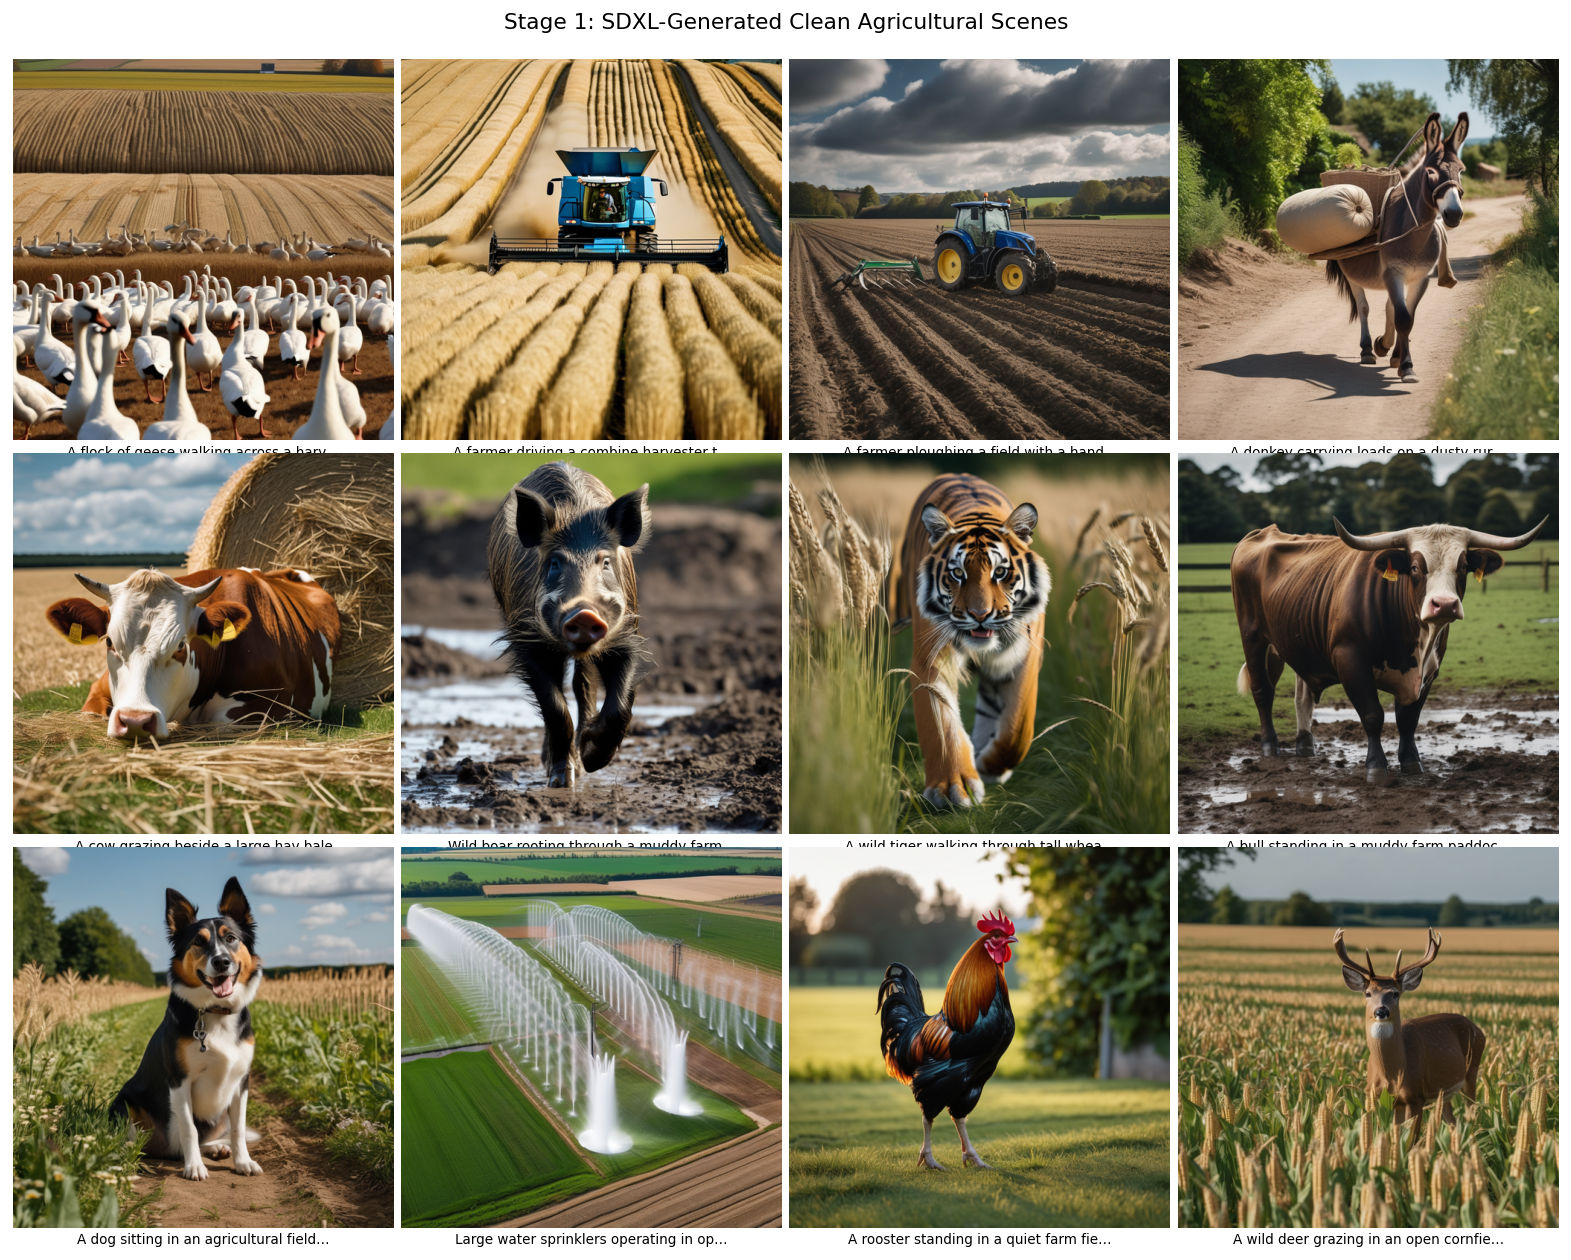
\includegraphics[width=0.85\linewidth]{images/agricultural_prompts_grid.png}
    \caption{Representative clean agricultural scenes generated in Stage~1. These 45 scenes form the content pool for all atmospheric style applications in Stages~2 and~3.}
    \label{fig:agricultural_prompts_grid}
\end{figure}

\FloatBarrier
% =====================================================
\section{Style Transfer Configurations (V1--V4)}
\label{sec:stage2_style}

\noindent Stage~2 applies an atmospheric style transfer pass on each clean scene. Four progressively refined pipeline configurations (V1--V4) were developed and compared, building on each other iteratively. V1 and V2 use style transfer alone; V3 and V4 additionally invoke the Stage~3 physics compositor, making them full three-stage pipeline variants. V4 was subsequently discarded due to destructive interference artefacts; V3 is the primary physics-grounded baseline. Table~\ref{tab:version_naming} provides the formal nomenclature for all versions; Table~\ref{tab:stage2_evolution} summarises how the Stage~2 architecture evolved. All version codes throughout this chapter refer to Table~\ref{tab:version_naming}.

\begin{table}[htbp]
\centering
\caption{Stage~2 architecture evolution across pipeline versions. CLIP confidence (ViT-L-14) is the mean softmax score on generated outputs — lower = stronger domain shift from clean. V4 was abandoned due to destructive interference artefacts. V3 and V9 are the final pipelines used in evaluation.}
\label{tab:stage2_evolution}
\resizebox{\textwidth}{!}{%
\small
\setlength{\tabcolsep}{4.5pt}
\begin{tabular}{lcccc}
\toprule
\textbf{Component} & \textbf{V1} & \textbf{V2}
  & \cellcolor{green!8}\textbf{V3 (Final)}
  & \cellcolor{teal!8}\textbf{V9 (Best)} \\
\midrule
IP-Adapter blocks
  & All (down+mid+up) & up$_{0}$+up$_{1}$
  & \cellcolor{green!8}up$_{0}$+up$_{1}$
  & \cellcolor{teal!8}up$_{0}$+up$_{1}$+mid \\
IP scale
  & 0.50 & 0.75
  & \cellcolor{green!8}0.85--0.88 & \cellcolor{teal!8}0.95 \\
img2img strength
  & 0.65 & 0.65
  & \cellcolor{green!8}0.70--0.74 & \cellcolor{teal!8}--- (pure t2i) \\
CSD guidance
  & $\checkmark$\ ($\eta$=0.18) & $\checkmark$\ ($\eta$=0.18)
  & \cellcolor{green!8}$\times$\ (removed) & \cellcolor{teal!8}$\checkmark$\ ($\eta$=0.25, $w$=1.5) \\
Spatial noise map
  & $\checkmark$ & $\times$
  & \cellcolor{green!8}$\times$ & \cellcolor{teal!8}$\times$ \\
Content subtraction
  & $\times$ & $\times$
  & \cellcolor{green!8}$\times$
  & \cellcolor{teal!8}$\checkmark$\ (CLIP ZS, $\alpha$=0.45) \\
Stage~3 compositor
  & Koschmieder & Koschmieder
  & \cellcolor{green!8}Koschmieder + high$\beta$
  & \cellcolor{teal!8}haze$\rightarrow$V3 / sand$\rightarrow$V5 Mie / snow$\rightarrow$V7 \\
\midrule
CLIP confidence $\downarrow$
  & 0.299 & 0.317
  & \cellcolor{green!8}\textbf{0.274}
  & \cellcolor{teal!8}\textbf{0.228} \\
Status
  & Superseded & Superseded
  & \cellcolor{green!8}Final dataset
  & \cellcolor{teal!8}Best pipeline \\
\bottomrule
\end{tabular}
}
\end{table}


\FloatBarrier
% -------------------------------------------------------
\begin{table}[htbp]
\centering
\caption{Version naming reference: internal codes, descriptions, and proposed formal names. All subsequent sections use the internal codes (V0--V9); this table provides the full nomenclature for cross-referencing.}
\label{tab:version_naming}
\small
\setlength{\tabcolsep}{5pt}
\renewcommand{\arraystretch}{1.3}
\begin{tabular}{@{}llp{6.2cm}@{}}
\toprule
\textbf{Code} & \textbf{Internal Description} & \textbf{Proposed Formal Name} \\
\midrule
V0  & InstantStyle + CSD Guidance                    & CSD-Guided Latent Optimisation \\
V1  & Global Style Injection + Depth-Modulated Noise & Depth-Aware Global Haze Injection \\
V2  & Style-Block Injection + Perceptual Guidance    & Block-Selective Perceptual Style Transfer \\
V3  & Style-Block Injection + Koschmieder            & Physics-Grounded Atmospheric Compositing \\
V4  & CSD + Koschmieder (Discarded)                  & CSD--Physics Hybrid Fusion (ablated) \\
V5  & Sandstorm Wavelength-Dependent Scattering      & Mie-Scattering Sandstorm Synthesis \\
V6  & Procedural Snowfall Simulation                 & Procedural Snowfall Particle Rendering \\
V7  & Snow Accumulation Modelling                    & Layered Winter Scene Synthesis \\
V9  & CLIP Subtraction + Koschmieder                 & Semantic-Decoupled Atmospheric Style Transfer \\
\bottomrule
\end{tabular}
\end{table}

\FloatBarrier
% -------------------------------------------------------
\subsection{V1: Global Style Injection with Depth-Modulated Noise}
\label{sec:v1}

\noindent V1~(Table~\ref{tab:version_naming}) was the starting point: IP-Adapter with all-block injection (not block-selective) combined with a spatially non-uniform noise map. The rationale was that all-block injection provides stronger style transfer, and the spatial noise map compensates for the lack of depth-awareness by explicitly modulating noise intensity by scene depth.

\paragraph{Configuration}
\begin{itemize}
    \item IP-Adapter injection: ALL blocks (down, mid, up), scale = 0.50.
    \item Spatial noise map: $s(x) = 0.55 + 0.20 \cdot w_\mathrm{depth}(x)$, where $w_\mathrm{depth}(x)$ is the normalised inverse depth (deeper $\rightarrow$ higher noise addition).
    \item CSD guidance: $\eta = 0.18$, applied every 3 steps.
    \item Style references: 3 domains — haze, sandstorm, snow.
\end{itemize}

\paragraph{Observations}
V1~(Table~\ref{tab:version_naming}) produced visually appealing atmospheric scenes but retained layout leakage and semantic drift from all-block injection. The ViT-L-14 confidence dropped from 0.3412 to 0.2978, indicating a modest domain shift.

\begin{figure}[htbp]
    \centering
    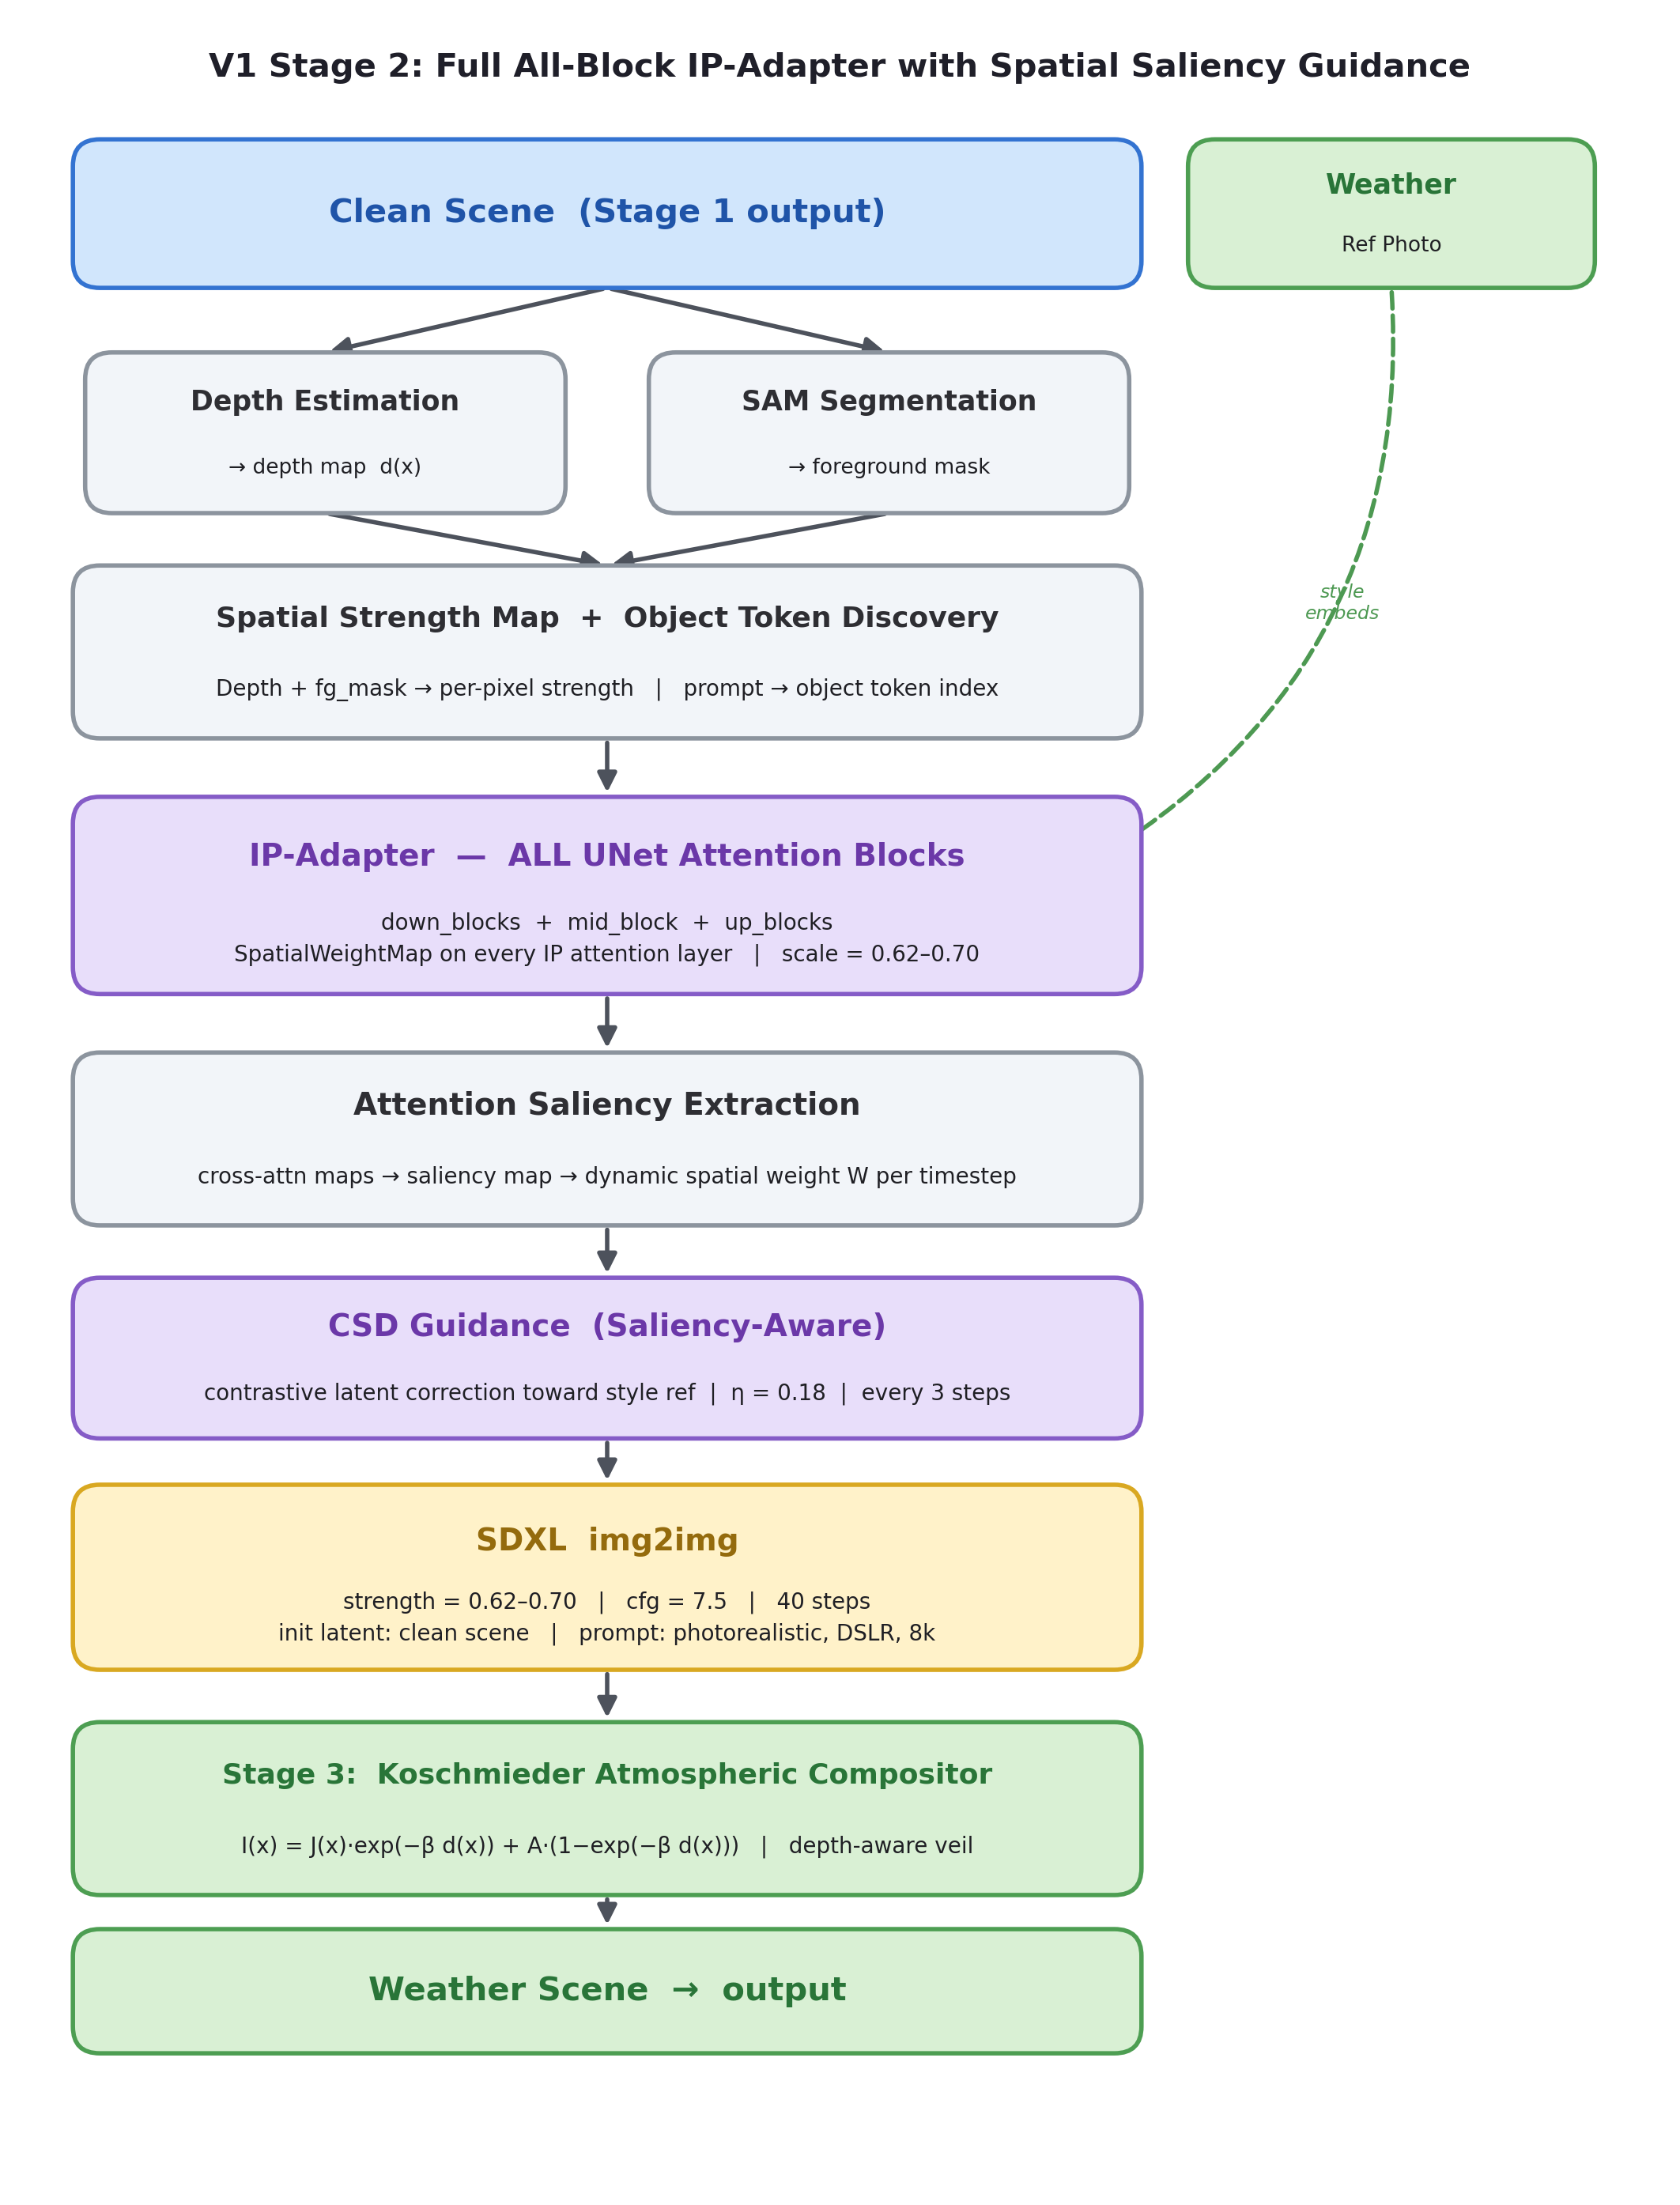
\includegraphics[width=0.82\linewidth]{images/arch_v1_stage2.png}
    \caption{V1 Stage~2 architecture. IP-Adapter injects style features into \emph{all} UNet blocks (\texttt{down\_blocks}, \texttt{mid\_block}, \texttt{up\_blocks}) at a uniform scale of 0.50. A spatially-varying noise map modulates denoising strength per pixel, and CSD gradient guidance is applied every 3 denoising steps. The key failure mode --- semantic leakage from the \texttt{mid\_block} (which encodes object identity) into the generated content --- motivated the block-selective injection approach adopted in V2 and V3. (Figure adapted from the Phase~2 Pipeline Architecture reference document.)}
    \label{fig:arch_v1_stage2}
\end{figure}

\FloatBarrier
% -------------------------------------------------------
\subsection{V2: Style-Block Injection with Perceptual Guidance}
\label{sec:v2}

\noindent V2~(Table~\ref{tab:version_naming}) switched to the block-selective InstantStyle injection (matching the proposed method from Chapter~\ref{chap:adaptive_proposed}) and increased the injection scale to compensate for the narrower injection scope.

\paragraph{Configuration}
\begin{itemize}
    \item IP-Adapter injection: \texttt{up\_blocks.0} and \texttt{up\_blocks.1} only (block-selective).
    \item Style injection scale: 0.75 (haze), 0.78 (sandstorm), 0.72 (snow).
    \item Img2img strength (denoising ratio): 0.62--0.70.
    \item CSD guidance: $\eta = 0.15$--$0.18$ (domain-specific), every 3 steps.
\end{itemize}

\paragraph{Observations}
V2~(Table~\ref{tab:version_naming}) preserved content semantic structure significantly better than V1. The ViT-L-14 zero-shot confidence on V2~(Table~\ref{tab:version_naming}) outputs was 0.3162 — actually slightly \emph{higher} than V1 (0.2978), indicating that V2's style transfer was more semantically transparent: the images looked more like stylised clean scenes and less like genuinely shifted domains. However, the Top-1 classification accuracy on V2 outputs was high: 93.3\% on haze, 94.1\% on sandstorm, 99.3\% on snow, and 96.0\% overall. This confirmed a known issue: block-selective injection produces high-quality-looking style transfer but the feature-space shift is insufficient for training robust vision models.

\FloatBarrier
% -------------------------------------------------------
\subsection{V3: Style-Block Injection with Physics Compositing}
\label{sec:v3}

\noindent V3~(Table~\ref{tab:version_naming}) was motivated by the observation that CSD guidance, while improving visual realism, does not meaningfully increase the feature-space domain shift beyond what InstantStyle alone achieves. Removing CSD guidance and using a minimal, generic text prompt (rather than a detailed agricultural description) was expected to reduce the model's tendency to ``fight back'' against the style transfer with its own prior knowledge of what agricultural scenes look like.

\paragraph{Configuration}
\begin{itemize}
    \item IP-Adapter injection: \texttt{up\_blocks.0} and \texttt{up\_blocks.1} only.
    \item Style injection scale: 0.85 (haze), 0.88 (sandstorm), 0.82 (snow) — higher than V2.
    \item Img2img strength: 0.72--0.74 (higher denoising ratio than V2, allowing more style influence).
    \item CSD guidance: \textbf{none}.
    \item Text prompt: minimal generic prompt (e.g., ``outdoor scene, atmospheric'') rather than detailed agricultural description.
    \item Koschmieder Stage~3 compositor: applied after style transfer (see Section~\ref{sec:stage3_physics}).
\end{itemize}

\paragraph{Observations}
V3~(Table~\ref{tab:version_naming}) achieved the strongest feature-space shift. Top-1 classification accuracy on V3~(Table~\ref{tab:version_naming}) outputs was 67.2\% (ViT-L-14) and 67.4\% (ViT-H-14) — well below the near-perfect accuracy on clean scenes and below V2's 96.0\%/95.3\%. The ViT-L-14 zero-shot confidence was 0.2744 — the lowest of all three versions, and noticeably below the clean scene confidence of 0.3416. The removal of CSD guidance made the images slightly less visually polished (some colour banding and texture inconsistency that CSD would have smoothed), but this was an acceptable trade-off for the stronger domain shift. V3 became the primary training data source for the downstream experiments.

\begin{figure}[htbp]
    \centering
    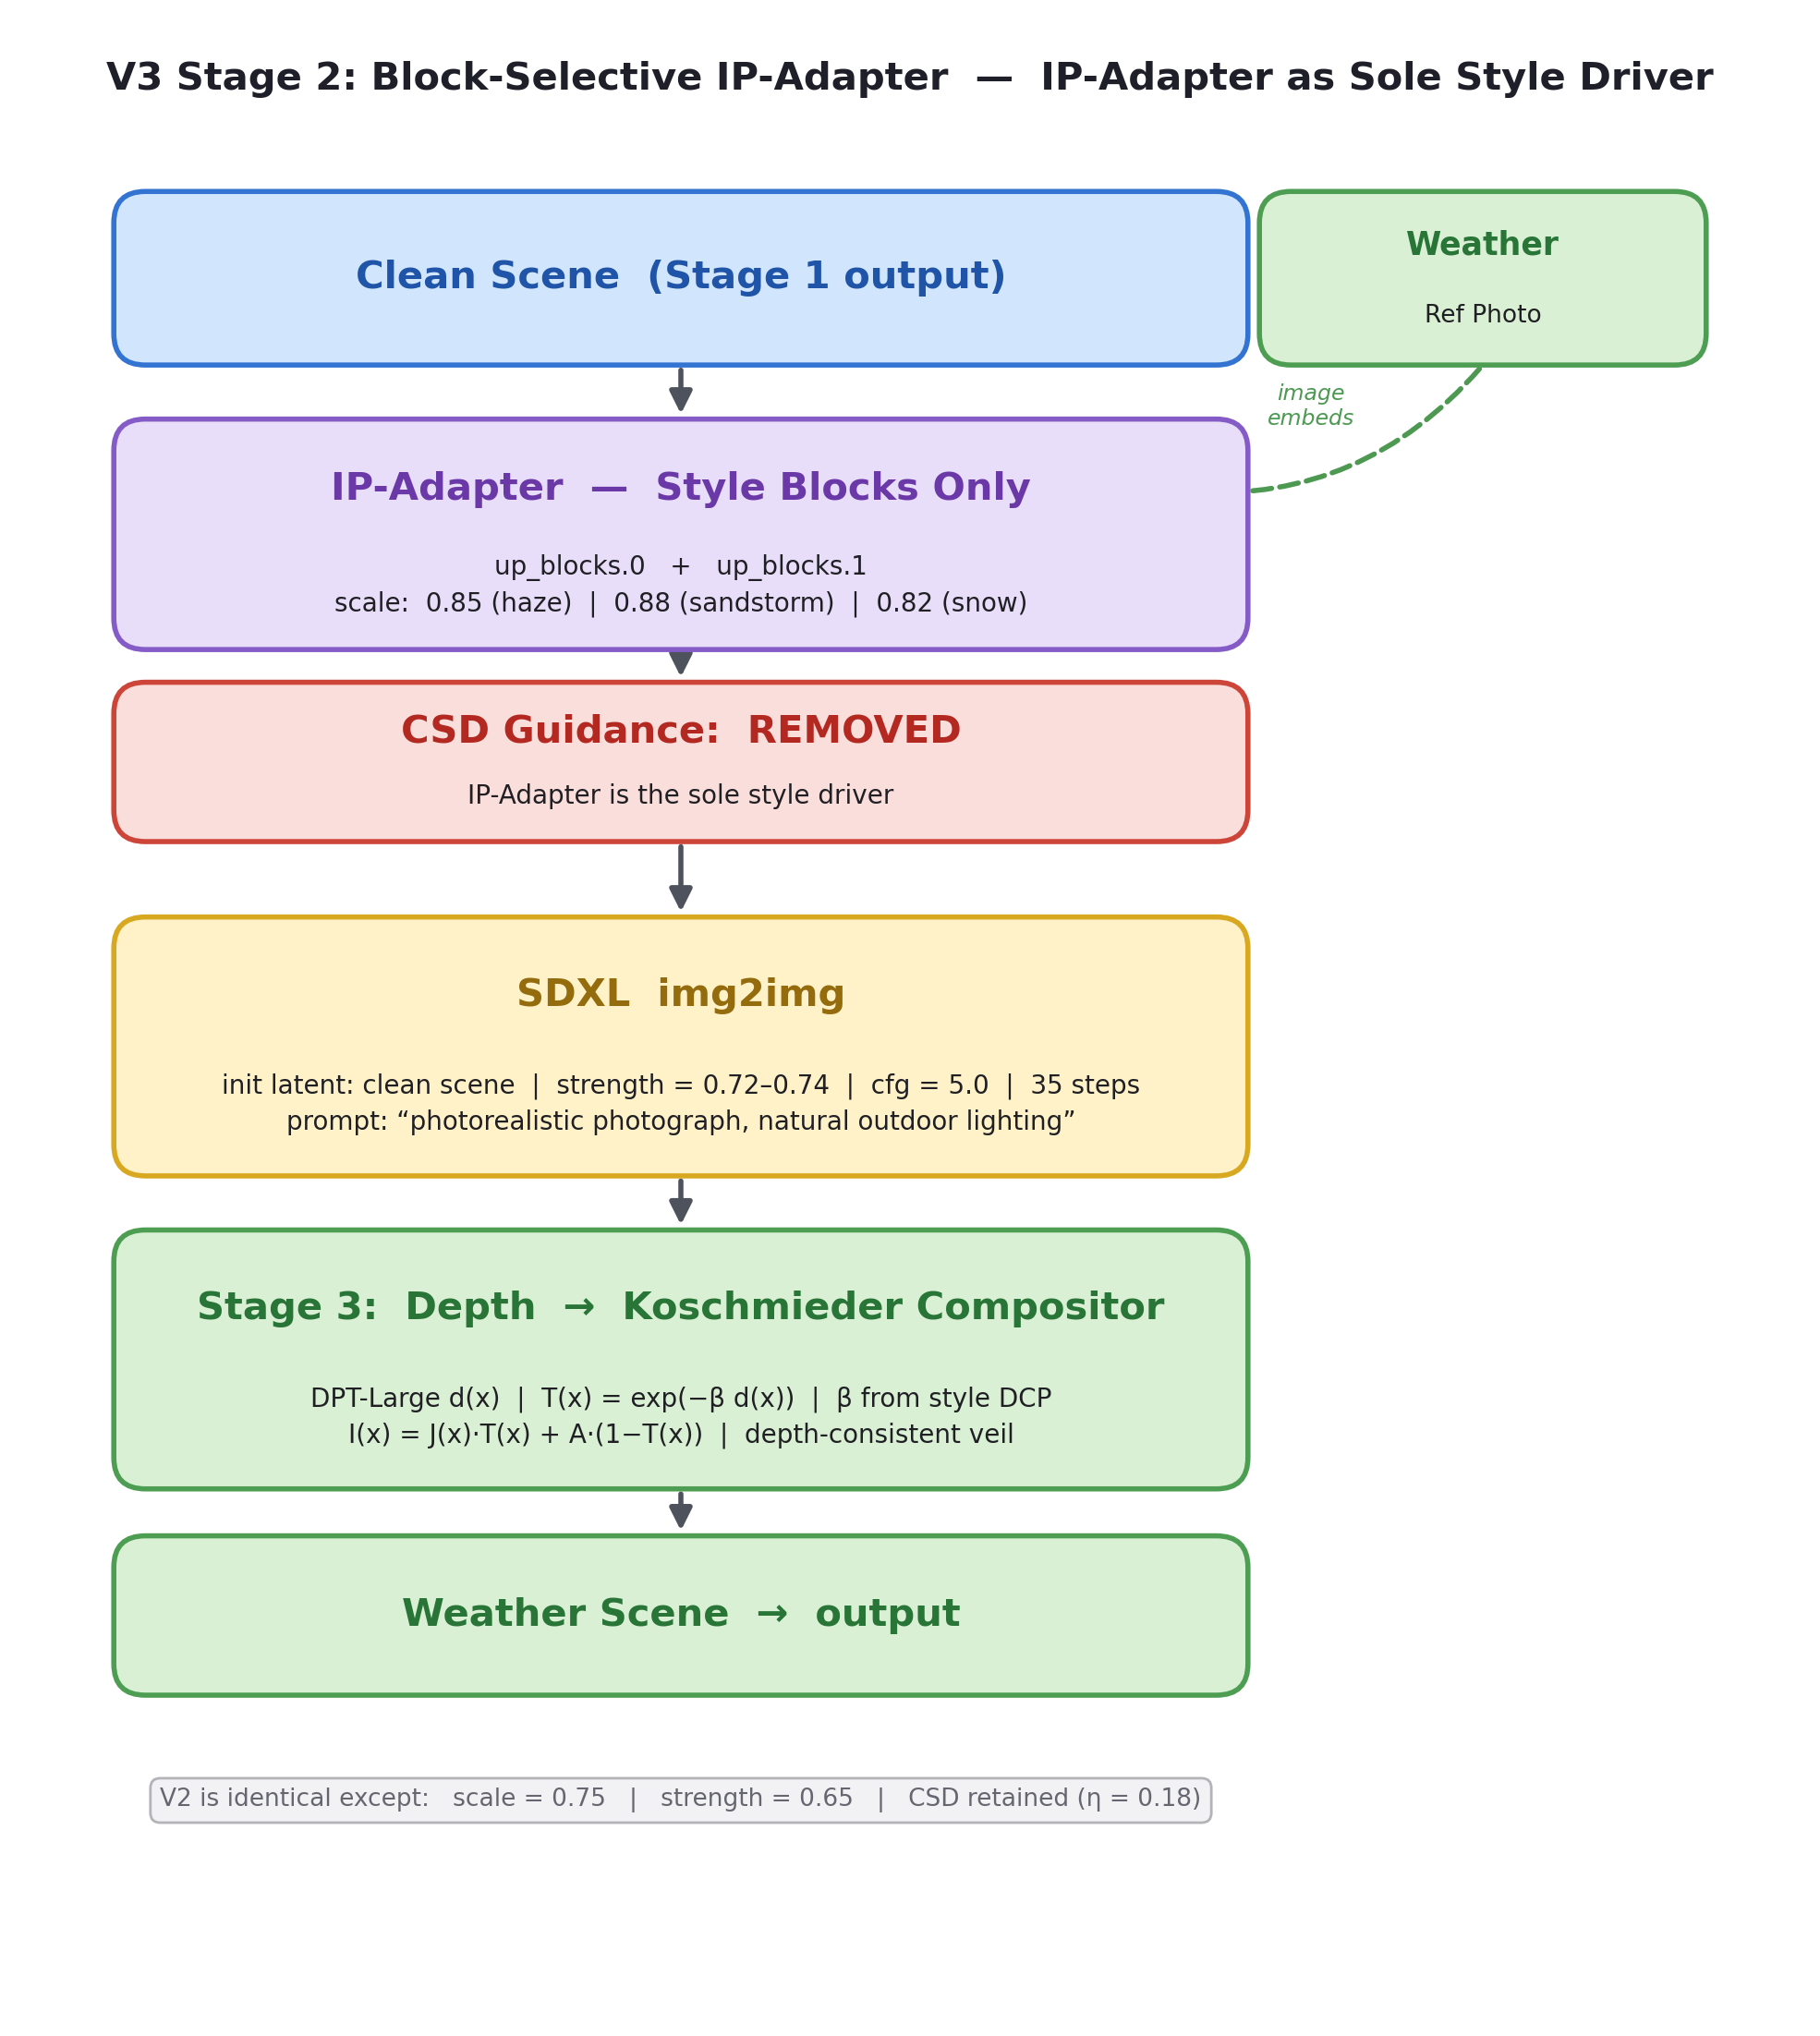
\includegraphics[width=0.80\linewidth]{images/arch_v3_stage2.png}
    \caption{V3 Stage~2 architecture (final pipeline). Block injection is restricted to \texttt{up\_blocks.0} and \texttt{up\_blocks.1} (scale\,=\,0.85--0.88 per domain), eliminating semantic leakage from the structural blocks. CSD guidance is \textbf{removed}: IP-Adapter is the sole style driver. A minimal generic prompt (``photorealistic photograph, natural outdoor lighting'') is used to prevent SDXL's text conditioning from competing with the image-style signal. Higher denoising strength (0.72--0.74) commits more fully to weather style than V2. The V2 architecture is identical except for lower scale (0.75), lower denoising strength (0.65), and CSD guidance retained ($\eta=0.18$). (Figure adapted from the Phase~2 Pipeline Architecture reference document.)}
    \label{fig:arch_v3_stage2}
\end{figure}

\begin{figure}[htbp]
    \centering
    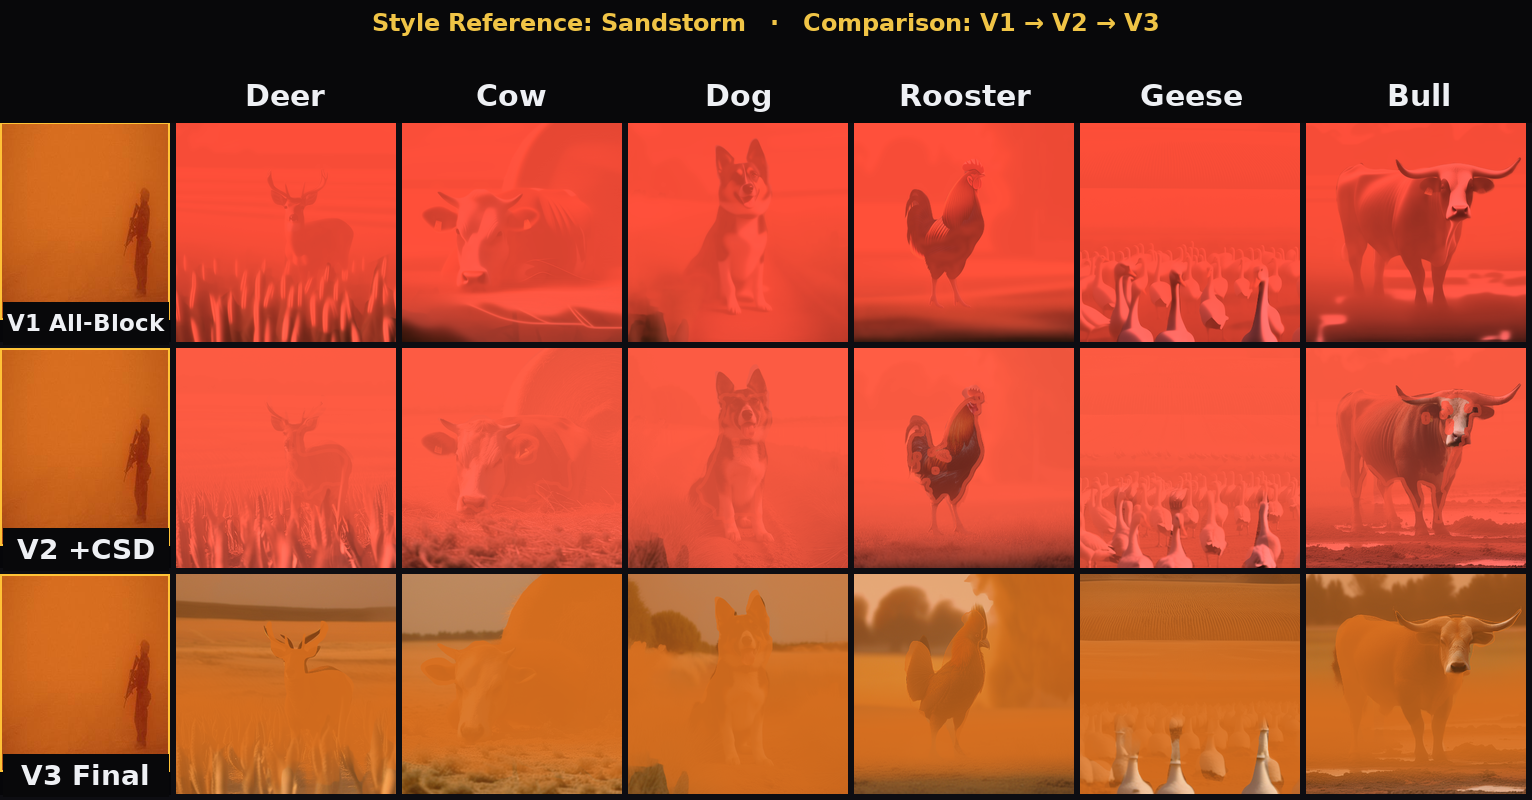
\includegraphics[width=0.97\linewidth]{images/v1_v2_v3_comparison.png}
    \caption{Pipeline comparison: V1 (all-block injection), V2 (block-selective + CSD), and V3 (block-selective, no CSD) applied to six content prompts using the same sandstorm style reference. Each row shows outputs from one pipeline version; columns are different agricultural scenes. V3 achieves the strongest atmospheric character.}
    \label{fig:v1_v2_v3_comparison}
\end{figure}

\paragraph{Dataset Scale}
45 clean scenes $\times$ 3 atmospheric styles $\times$ 3 versions = 405 images total. The full V3 dataset (405 images across all domains) was used for Experiments 1--3.

\paragraph{V3-HighBeta Variant}
\label{sec:v3_highbeta}
To probe the sensitivity of depth-coherence to the Koschmieder scattering coefficient, a single ablation variant of V3 --- designated \textbf{V3-HighBeta} --- was generated using twice the nominal scattering coefficient ($\beta_{\mathrm{HB}} = 2\beta_{\mathrm{V3}}$). All other V3 hyperparameters were held constant; only the Koschmieder compositor received the elevated $\beta$ value. The stronger extinction coefficient substantially increases the physical haze density at depth, producing images where distant objects are almost entirely occluded. This variant was not used as training data for downstream experiments but was included in the metrics study (Section~\ref{sec:proposed_metrics}) to establish how increasing the scattering coefficient $\beta$ degrades subject visibility, serving as an upper-bound reference for atmospheric strength.

\FloatBarrier
% -------------------------------------------------------
\subsection{V4: CSD + Koschmieder (Discarded)}
\label{sec:v4_discarded}

\noindent V4~(Table~\ref{tab:version_naming}) was an attempt to combine V3's Koschmieder physics compositor with CSD guidance reintroduced at the latent level, testing whether active perceptual correction could further refine the style signal on top of physics-grounded compositing.

\noindent Qualitative inspection of the V4~(Table~\ref{tab:version_naming}) outputs immediately revealed severe artefacts across all three atmospheric domains. Haze samples exhibited pronounced red/cyan chromatic aberration — bright red halos around every subject edge and cyan fringing in shadows, resembling a 3D anaglyph image viewed without glasses. In several farmland samples, content drifted entirely (SDXL hallucinated unrelated scenery such as waterfalls). Sandstorm samples showed teal--orange colour channel separation, producing a duotone or thermal-imaging appearance rather than the warm, uniform particulate characteristic of sandstorm imagery. Snow samples displayed a strong green cast with no visible snow effect — CSD had pushed the latents in the opposite direction from the cold white/blue snow style reference.

\paragraph{Why the failure occurs}
CSD applies gradient corrections at the latent level every 3 denoising steps, while IP-Adapter injects style via cross-attention simultaneously. At V3's high denoising strength (0.78--0.85), approximately 27 active denoising steps remain, yielding $\sim$9 CSD corrections per image. These corrections compound: the accumulated colour shifts manifest as chromatic aberration and channel separation visible in every domain. The two objectives compete directly — IP-Adapter pulls cross-attention features toward the weather style while CSD simultaneously pushes latents toward the CSD style descriptor. At this denoising strength, neither wins cleanly, producing destructive interference. This contrasts with V2, where the weaker denoising strength (0.65) permitted partial coexistence of the two signals.

\noindent V4~(Table~\ref{tab:version_naming}) was discarded after the qualitative inspection. The artefacts are visually unambiguous and constitute strong evidence that the V3 design choice — IP-Adapter as the sole style driver with no competing gradient objectives — is the correct architecture for weather transfer at committed denoising strengths.

\FloatBarrier
% =====================================================
\section{Stage 3: Physics-Grounded Atmospheric Compositor}
\label{sec:stage3_physics}

\noindent Stage~3 takes each style-transferred image from Stage~2 and applies a depth-aware physics compositor that enforces the Koschmieder atmospheric scattering law~\cite{koschmieder1924theorie}. This is the key innovation of the proposed pipeline: rather than asking a generative model to impose physical constraints (which the preceding style transfer experiments showed to be unreliable), the physics is applied as a deterministic post-processor.

\FloatBarrier
% -------------------------------------------------------
\subsection{Koschmieder Atmospheric Scattering Model}
\label{sec:koschmieder}

\noindent The Koschmieder model~\cite{koschmieder1924theorie} describes how an image $I(x)$ of a scene with radiance $J(x)$ is affected by atmospheric scattering:
\begin{equation}
    I(x) = J(x) \cdot T(x) + A \cdot (1 - T(x)),
    \label{eq:koschmieder}
\end{equation}
where:
\begin{itemize}
    \item $T(x) = \exp(-\beta \cdot D(x))$ is the \textbf{transmission map}: the fraction of scene radiance that survives to the camera.
    \item $D(x)$ is the scene depth at pixel $x$.
    \item $\beta$ is the \textbf{scattering coefficient}: larger $\beta$ means denser atmosphere.
    \item $A$ is the \textbf{atmospheric light} (airlight): the colour of the medium itself (white for haze, warm yellow-brown for sandstorm, blue-white for snow).
\end{itemize}

\noindent When $D(x)$ is large (distant object), $T(x) \rightarrow 0$ and $I(x) \rightarrow A$ — the object disappears into the atmospheric medium. When $D(x)$ is small (close object), $T(x) \rightarrow 1$ and $I(x) \rightarrow J(x)$ — the object is seen clearly. This is exactly the depth-dependent attenuation that was missing from all the style-transfer approaches in earlier experiments.

\FloatBarrier
% -------------------------------------------------------
\subsection{Depth Estimation with Intel DPT-Large}
\label{sec:dpt_depth}

\noindent Per-scene depth maps $D(x)$ were estimated using Intel DPT-Large~\cite{ranftl2021dpt}, a transformer-based monocular depth estimator. DPT-Large was run on each Stage~2 style-transferred image to produce a normalised depth map in $[0, 1]$. The scattering coefficient $\beta$ and atmospheric light $A$ were set per-domain:

\begin{itemize}
    \item \textbf{Haze:} $\beta = 1.5$--$3.0$, $A = [0.95, 0.95, 0.95]$ (near-white).
    \item \textbf{Sandstorm:} $\beta = 2.0$--$4.0$, $A = [0.90, 0.80, 0.60]$ (warm amber).
    \item \textbf{Snow:} $\beta = 1.0$--$2.5$, $A = [0.92, 0.94, 0.98]$ (cool blue-white).
\end{itemize}

\noindent These values were derived from the Dark Channel Prior method~\cite{he2009dark}, which estimates $\beta$ and $A$ from statistics of the style reference photographs in the curated dataset.

\FloatBarrier
% -------------------------------------------------------
\subsection{Three-Step Compositing Pipeline}
\label{sec:compositing}

\noindent The Stage~3 compositor applies three sequential operations:

\paragraph{Step 1: Atmospheric Veil (Koschmieder)}
The transmission map $T(x) = \exp(-\beta \cdot D(x))$ is computed from the DPT-Large depth map. Equation~\ref{eq:koschmieder} is then applied pixel-wise: $I(x) = J(x) \cdot T(x) + A \cdot (1 - T(x))$.

\paragraph{Step 2: Edge Dissolution}
Real atmospheric scenes exhibit softening of high-frequency edges in proportion to depth. A depth-weighted Gaussian blur is applied: $\sigma(x) = \sigma_\mathrm{max} \cdot (1 - T(x))$. Pixels in deeply attenuated regions (low $T$) receive more blur; foreground pixels receive minimal blur.

\paragraph{Step 3: Colour and Saturation Shift}
Atmospheric scattering affects colour channels non-uniformly. A channel-specific saturation reduction is applied, with the magnitude proportional to $(1 - T(x))$: pixels that are more heavily attenuated also receive stronger desaturation toward the atmospheric light colour $A$.

\begin{figure}[htbp]
    \centering
    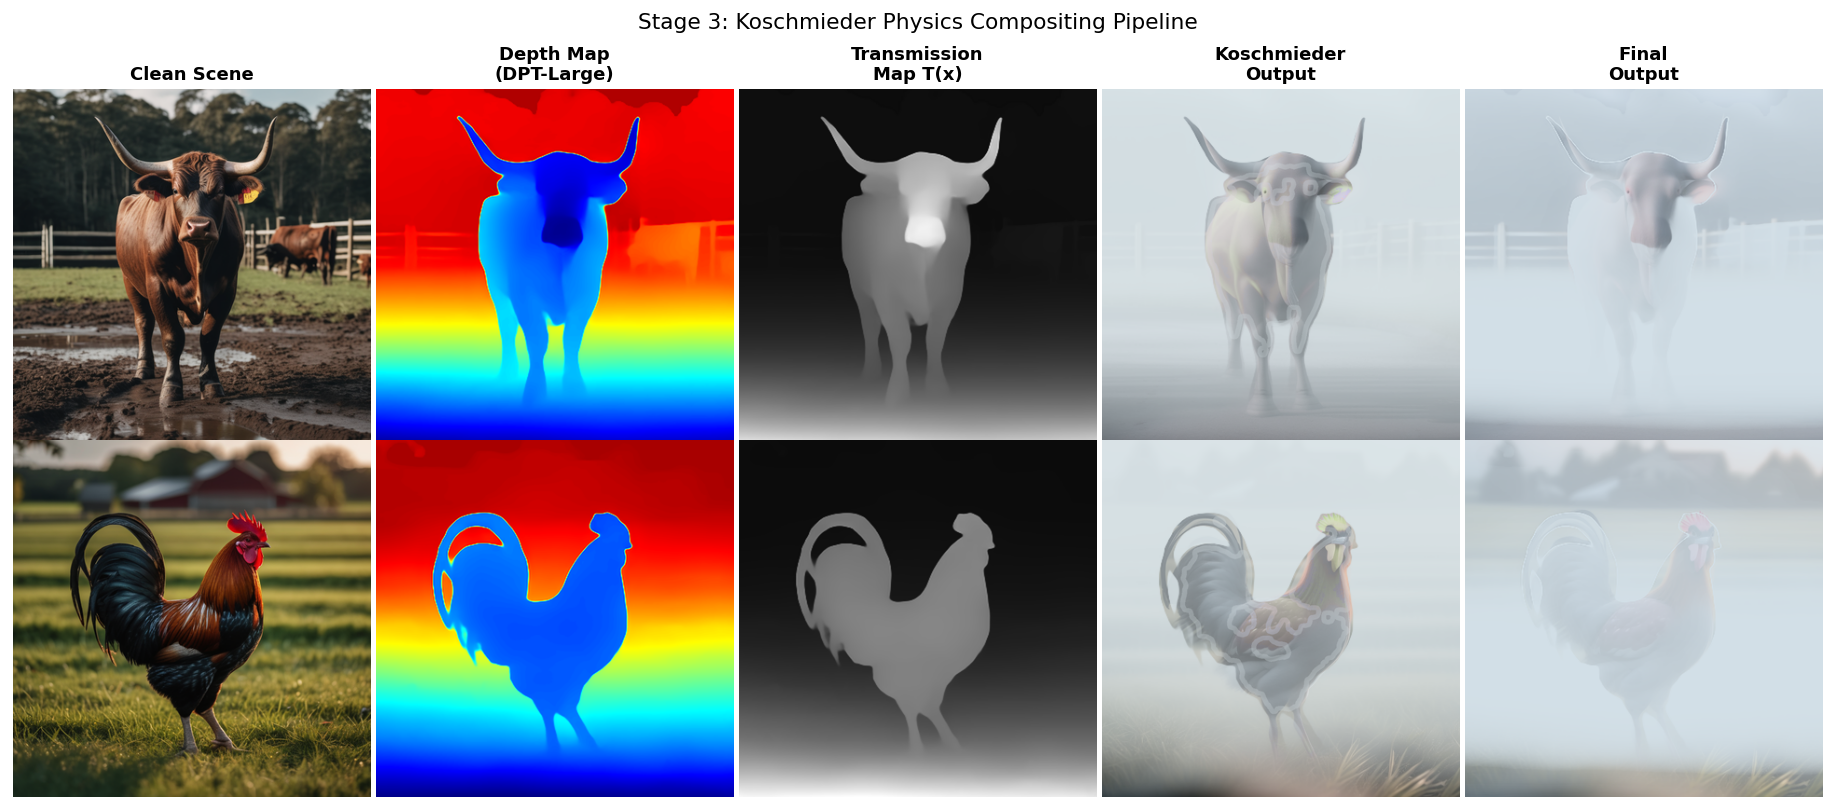
\includegraphics[width=0.97\linewidth]{images/koschmieder_depth_stages.png}
    \caption{Stage~3 physics compositing pipeline for a single example. Top row: clean scene, DPT-Large depth map, computed transmission map. Bottom row: Koschmieder output (Eq.~\ref{eq:koschmieder}), edge-dissolved version, final output with colour shift.}
    \label{fig:koschmieder_depth_stages}
\end{figure}

\FloatBarrier
% =====================================================
\section{KDA-Net: The Learned Compositor Attempt}
\label{sec:kda_net}

\noindent In parallel with the Koschmieder compositor, a learned neural compositor, KDA-Net, was designed and trained. The goal was to replace the hand-tuned Koschmieder parameters ($\beta$, $A$) with a network that learned to predict the appropriate atmospheric compositing parameters from the scene content and style reference, potentially handling cases where the simple Koschmieder model is insufficient (e.g., participating media with wavelength-dependent scattering).

\FloatBarrier
% -------------------------------------------------------
\subsection{Architecture}
\label{sec:kda_arch}

\noindent KDA-Net has two sub-networks:

\begin{itemize}
    \item \textbf{Haze Image Generator (HIG):} Three modules — Texture Encoder (TE), Haze Encoder (HE), and Image Compositor (IC). The HIG takes a clean scene and a haze style reference and outputs a composited hazy image using a learned transmission map $t^\theta$: $I_o = J_n \cdot t^\theta + A \cdot (1 - t^\theta)$, where $\theta$ are the predicted transmission parameters.
    \item \textbf{Haze Authenticator (HA):} Two patch discriminators — Content Identity (CI) and Haze Identity (HI) — that distinguish genuine atmospheric images from KDA-Net composites. The adversarial training was intended to prevent the HIG from producing atmospheric images that are obviously synthetic.
\end{itemize}

\begin{figure}[htbp]
    \centering
    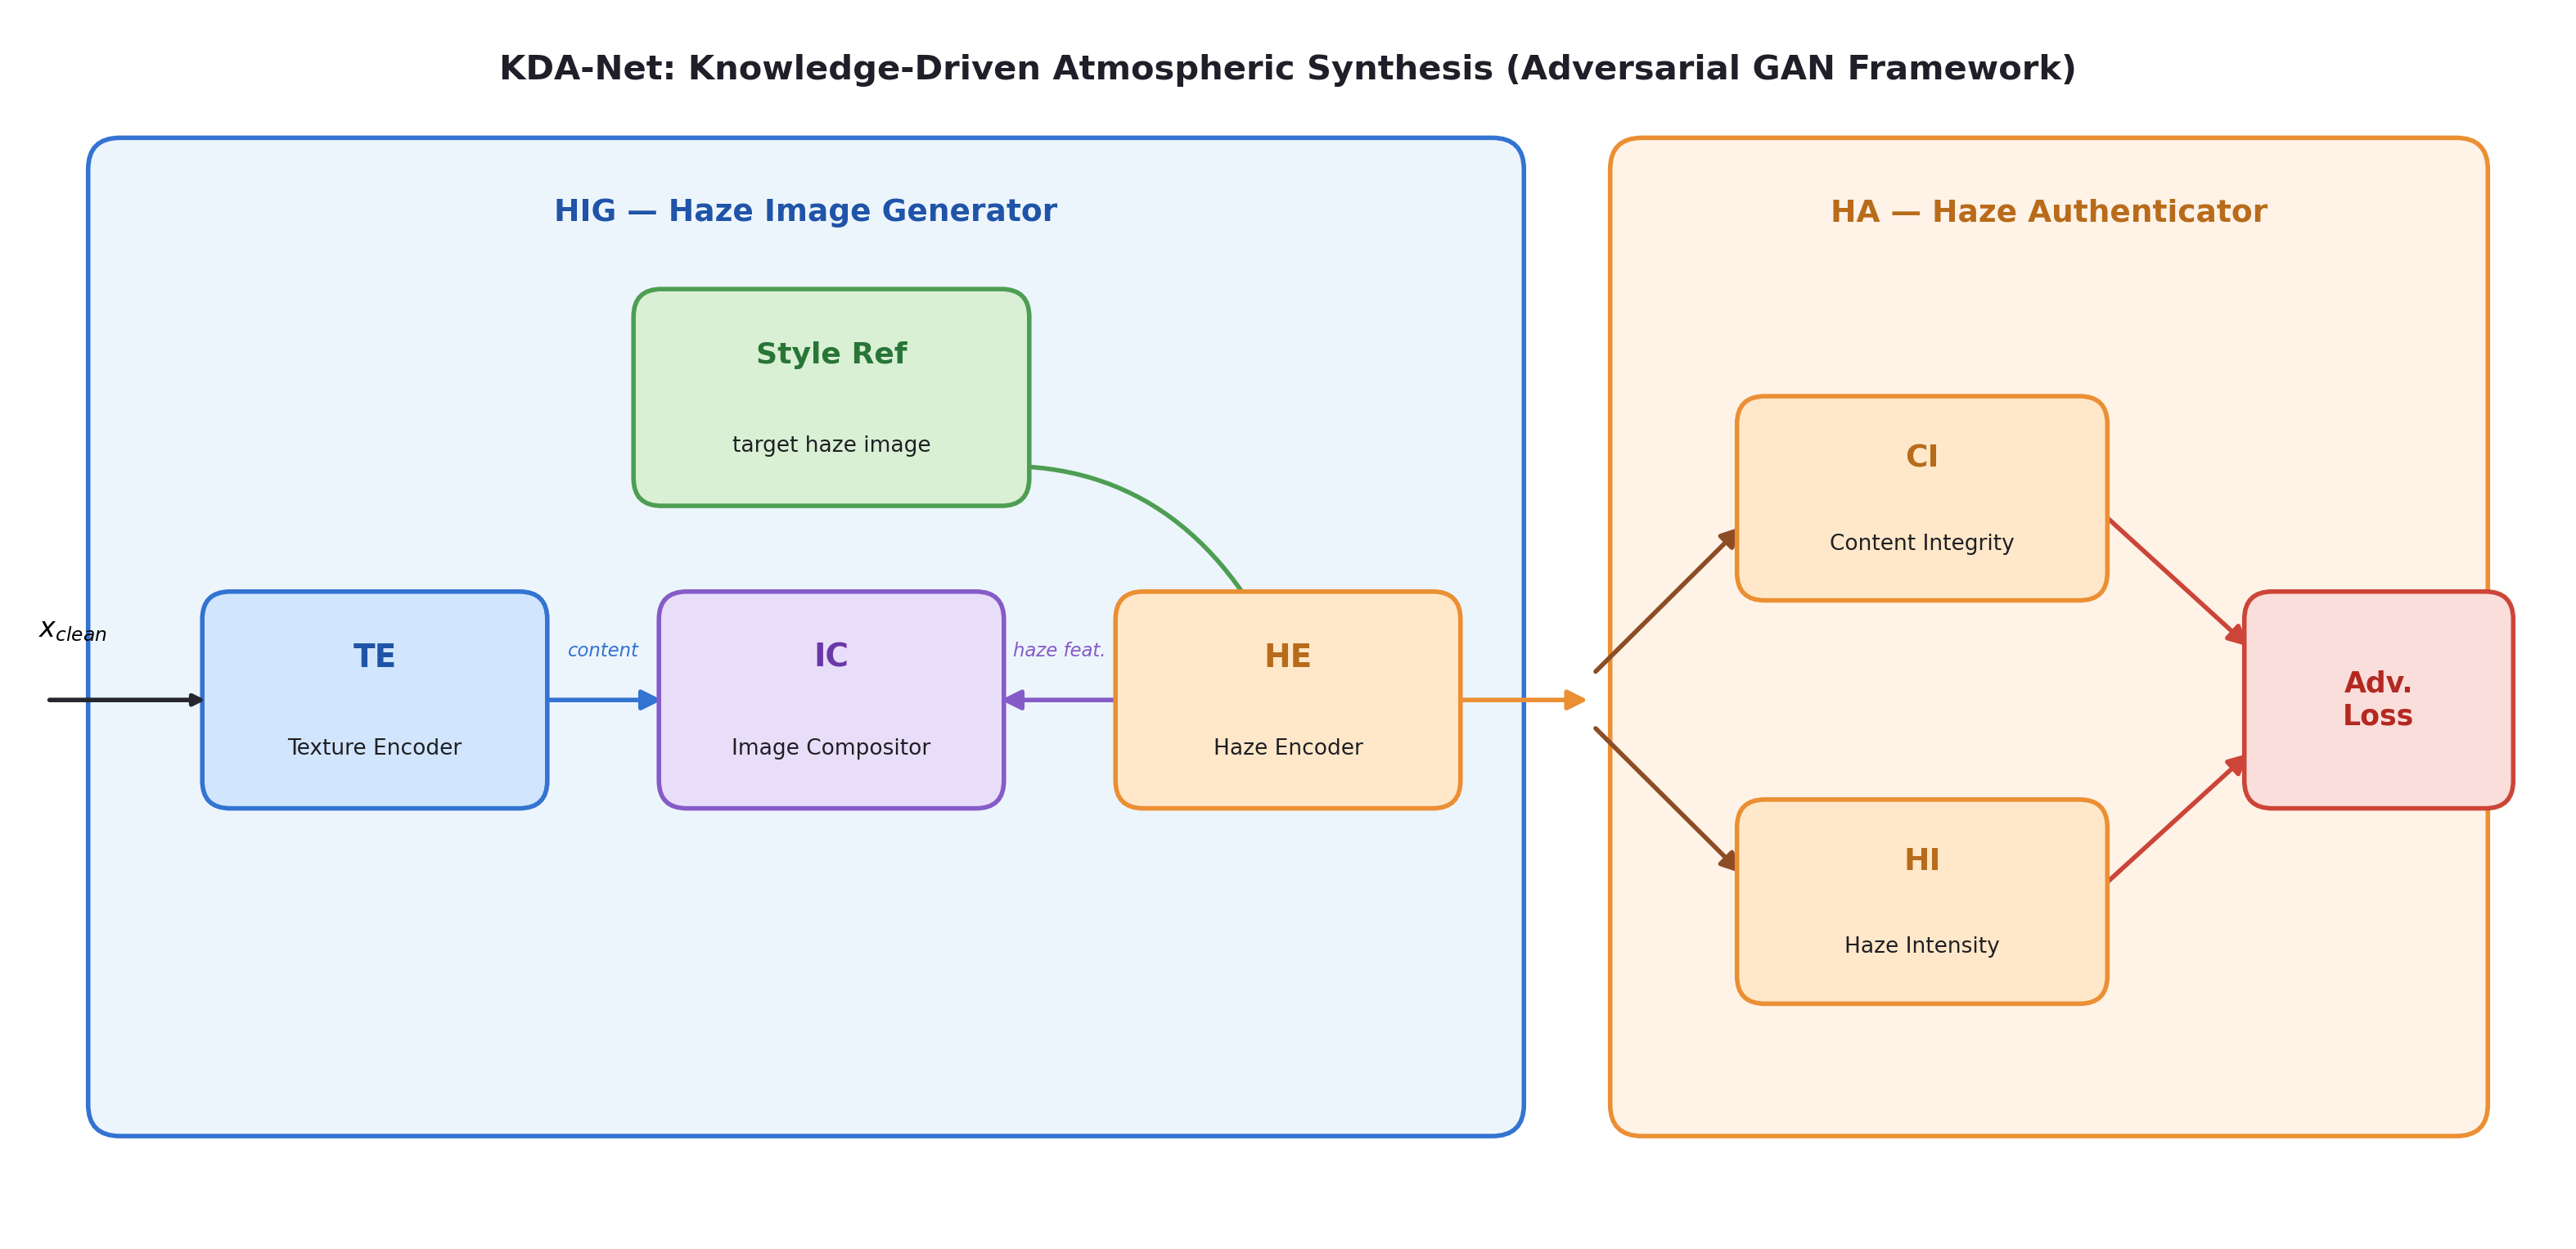
\includegraphics[width=0.97\linewidth]{images/kda_net_architecture.png}
    \caption{KDA-Net architecture: Haze Image Generator (HIG) with three modules (TE, HE, IC) and Haze Authenticator (HA) with two patch discriminators (CI, HI). The adversarial training was intended to enforce realism.}
    \label{fig:kda_net_architecture}
\end{figure}

\FloatBarrier
% -------------------------------------------------------
\subsection{Training and Failure}
\label{sec:kda_training}

\noindent KDA-Net was trained for 10--18 epochs without the GAN component (discriminators disabled) to first establish stable HIG outputs before introducing adversarial training. The non-adversarial training revealed a fundamental problem: the HIG converged to a solution with a persistent green colour cast across all outputs. The cause was traced to the IC module's learned blending weights, which systematically over-weighted the Haze Encoder features in the green channel. Without adversarial feedback from the HA to penalise this artefact, the HIG had no incentive to correct the colour distribution.

\noindent Attempts to fix the green cast through per-channel normalisation and colour loss terms were partially successful but did not eliminate it entirely. The adversarial training (re-enabled at epochs 15--18) was unstable: the CI discriminator collapsed early, and the HI discriminator overfit to the green cast rather than to genuine atmospheric texture. At 15:17 on June 5, 2025, the decision was made to restore the Koschmieder compositor as the Stage~3 standard and exclude KDA-Net outputs from all downstream experiments.

\noindent The KDA-Net architecture remains in the repository (\texttt{phase2\_pipeline/modules/kda\_net.py}) and the training code is intact. It represents a promising direction for future work: with a larger training dataset of real atmospheric images and extended adversarial training (50+ epochs), the colour cast could potentially be corrected and the learned compositor could surpass the simple Koschmieder model for complex atmospheric conditions.

\FloatBarrier
% =====================================================
\section{Complete Pipeline Parameter Tables}
\label{sec:pipeline_params}

\noindent Table~\ref{tab:v1_v2_v3_params} summarises all Stage~2 configuration parameters across V1--V4.

\begin{table}[htbp]
\centering
\caption{Complete parameter comparison across Stage~2 configurations V1--V4. V4 was discarded after qualitative inspection (see Section~\ref{sec:v4_discarded}); no quantitative metrics were collected.}
\label{tab:v1_v2_v3_params}
\renewcommand{\arraystretch}{1.3}
\resizebox{\textwidth}{!}{%
\begin{tabular}{lllll}
\toprule
\textbf{Parameter} & \textbf{V1} & \textbf{V2} & \textbf{V3} & \textbf{V4 (discarded)} \\
\midrule
IP-Adapter injection blocks & All (down+mid+up) & up\_blocks.0/1 only & up\_blocks.0/1 only & up\_blocks.0/1 only \\
IP-Adapter scale (haze) & 0.50 & 0.75 & 0.85 \\
IP-Adapter scale (sandstorm) & 0.50 & 0.78 & 0.88 \\
IP-Adapter scale (snow) & 0.50 & 0.72 & 0.82 \\
Img2img denoising strength & 0.60 & 0.62--0.70 & 0.72--0.74 & 0.72--0.74 \\
CSD guidance $\eta$ & 0.18 & 0.15--0.18 & None & 0.15 \\
CSD guidance interval & Every 3 steps & Every 3 steps & — & Every 3 steps \\
Koschmieder compositor & No & No & Yes & Yes \\
Text prompt & Detailed agricultural & Detailed agricultural & Minimal generic & Minimal generic \\
Spatial noise map & Yes ($s(x) = 0.55 + 0.20\,w_d$) & No & No & No \\
\midrule
ZS confidence (ViT-L-14) & 0.2978 & 0.3162 & 0.2740 & \textit{N/A (artefacts)} \\
Top-1 accuracy (ViT-L-14 / ViT-H-14) & — & 96.0\% / 95.3\% & 67.2\% / 67.4\% & \textit{N/A (artefacts)} \\
\bottomrule
\end{tabular}}
\end{table}


\FloatBarrier
% =====================================================
\section{Weather-Specific Physics Refinements}
\label{sec:weather_physics}

\noindent The V3 architecture established a stable foundation for atmospheric synthesis using the standard Koschmieder scattering model. However, further experimentation showed that some atmospheric phenomena require weather-specific physical modelling beyond a single extinction coefficient. Sandstorms are distinguished by large dust particles that scatter light differently across colour channels. Snowstorms add visible precipitation particles and surface accumulation that cannot be replicated by volumetric scattering alone.

\FloatBarrier
\subsection{V5: Sandstorm Wavelength-Dependent Scattering}
\label{sec:v5_sandstorm}

\noindent The classical Koschmieder model assumes a wavelength-independent extinction coefficient $\beta$. This assumption is sufficient for fog and haze, but does not reproduce the characteristic warm colour behaviour of sandstorms. Real sandstorms are dominated by mineral dust particles in the 1--100\,$\mu$m range, which scatter light in the Mie scattering regime. Unlike Rayleigh scattering (power-law exponent $\alpha \approx 4$, strongly wavelength-dependent), Mie scattering has $\alpha \approx 0.7$ — the attenuation varies only weakly with wavelength. However, even a small asymmetry across RGB channels is sufficient to produce the characteristic warm tint of airborne dust: blue is extinguished marginally faster than red, causing distant objects to shift toward amber-orange.

\noindent V5~(Table~\ref{tab:version_naming}) introduced channel-specific extinction coefficients calibrated to this regime:
\begin{equation}
    \beta_R = 0.87\,\beta, \qquad \beta_G = \beta, \qquad \beta_B = 1.15\,\beta.
\end{equation}

The full per-channel image formation model is applied independently for each colour channel $c \in \{R,G,B\}$:
\begin{equation}
    I_c(x) = J_c(x)\,e^{-\beta_c\,d(x)} + A_c\,\bigl(1 - e^{-\beta_c\,d(x)}\bigr),
\end{equation}
where $J_c(x)$ is the clean pixel value in channel $c$, $d(x)$ is the normalised scene depth from DPT-Large, and $A_c$ is the sandy atmospheric light colour ($A = [0.90,\,0.80,\,0.60]$ warm amber). Because $\beta_B > \beta_G > \beta_R$, the blue transmission decays fastest with depth. Distant objects progressively shift toward the sandy colour of the atmosphere; near objects retain their original colour. The result is a depth-consistent warm haze that cannot be reproduced by a single-channel compositor.

\begin{figure}[htbp]
    \centering
    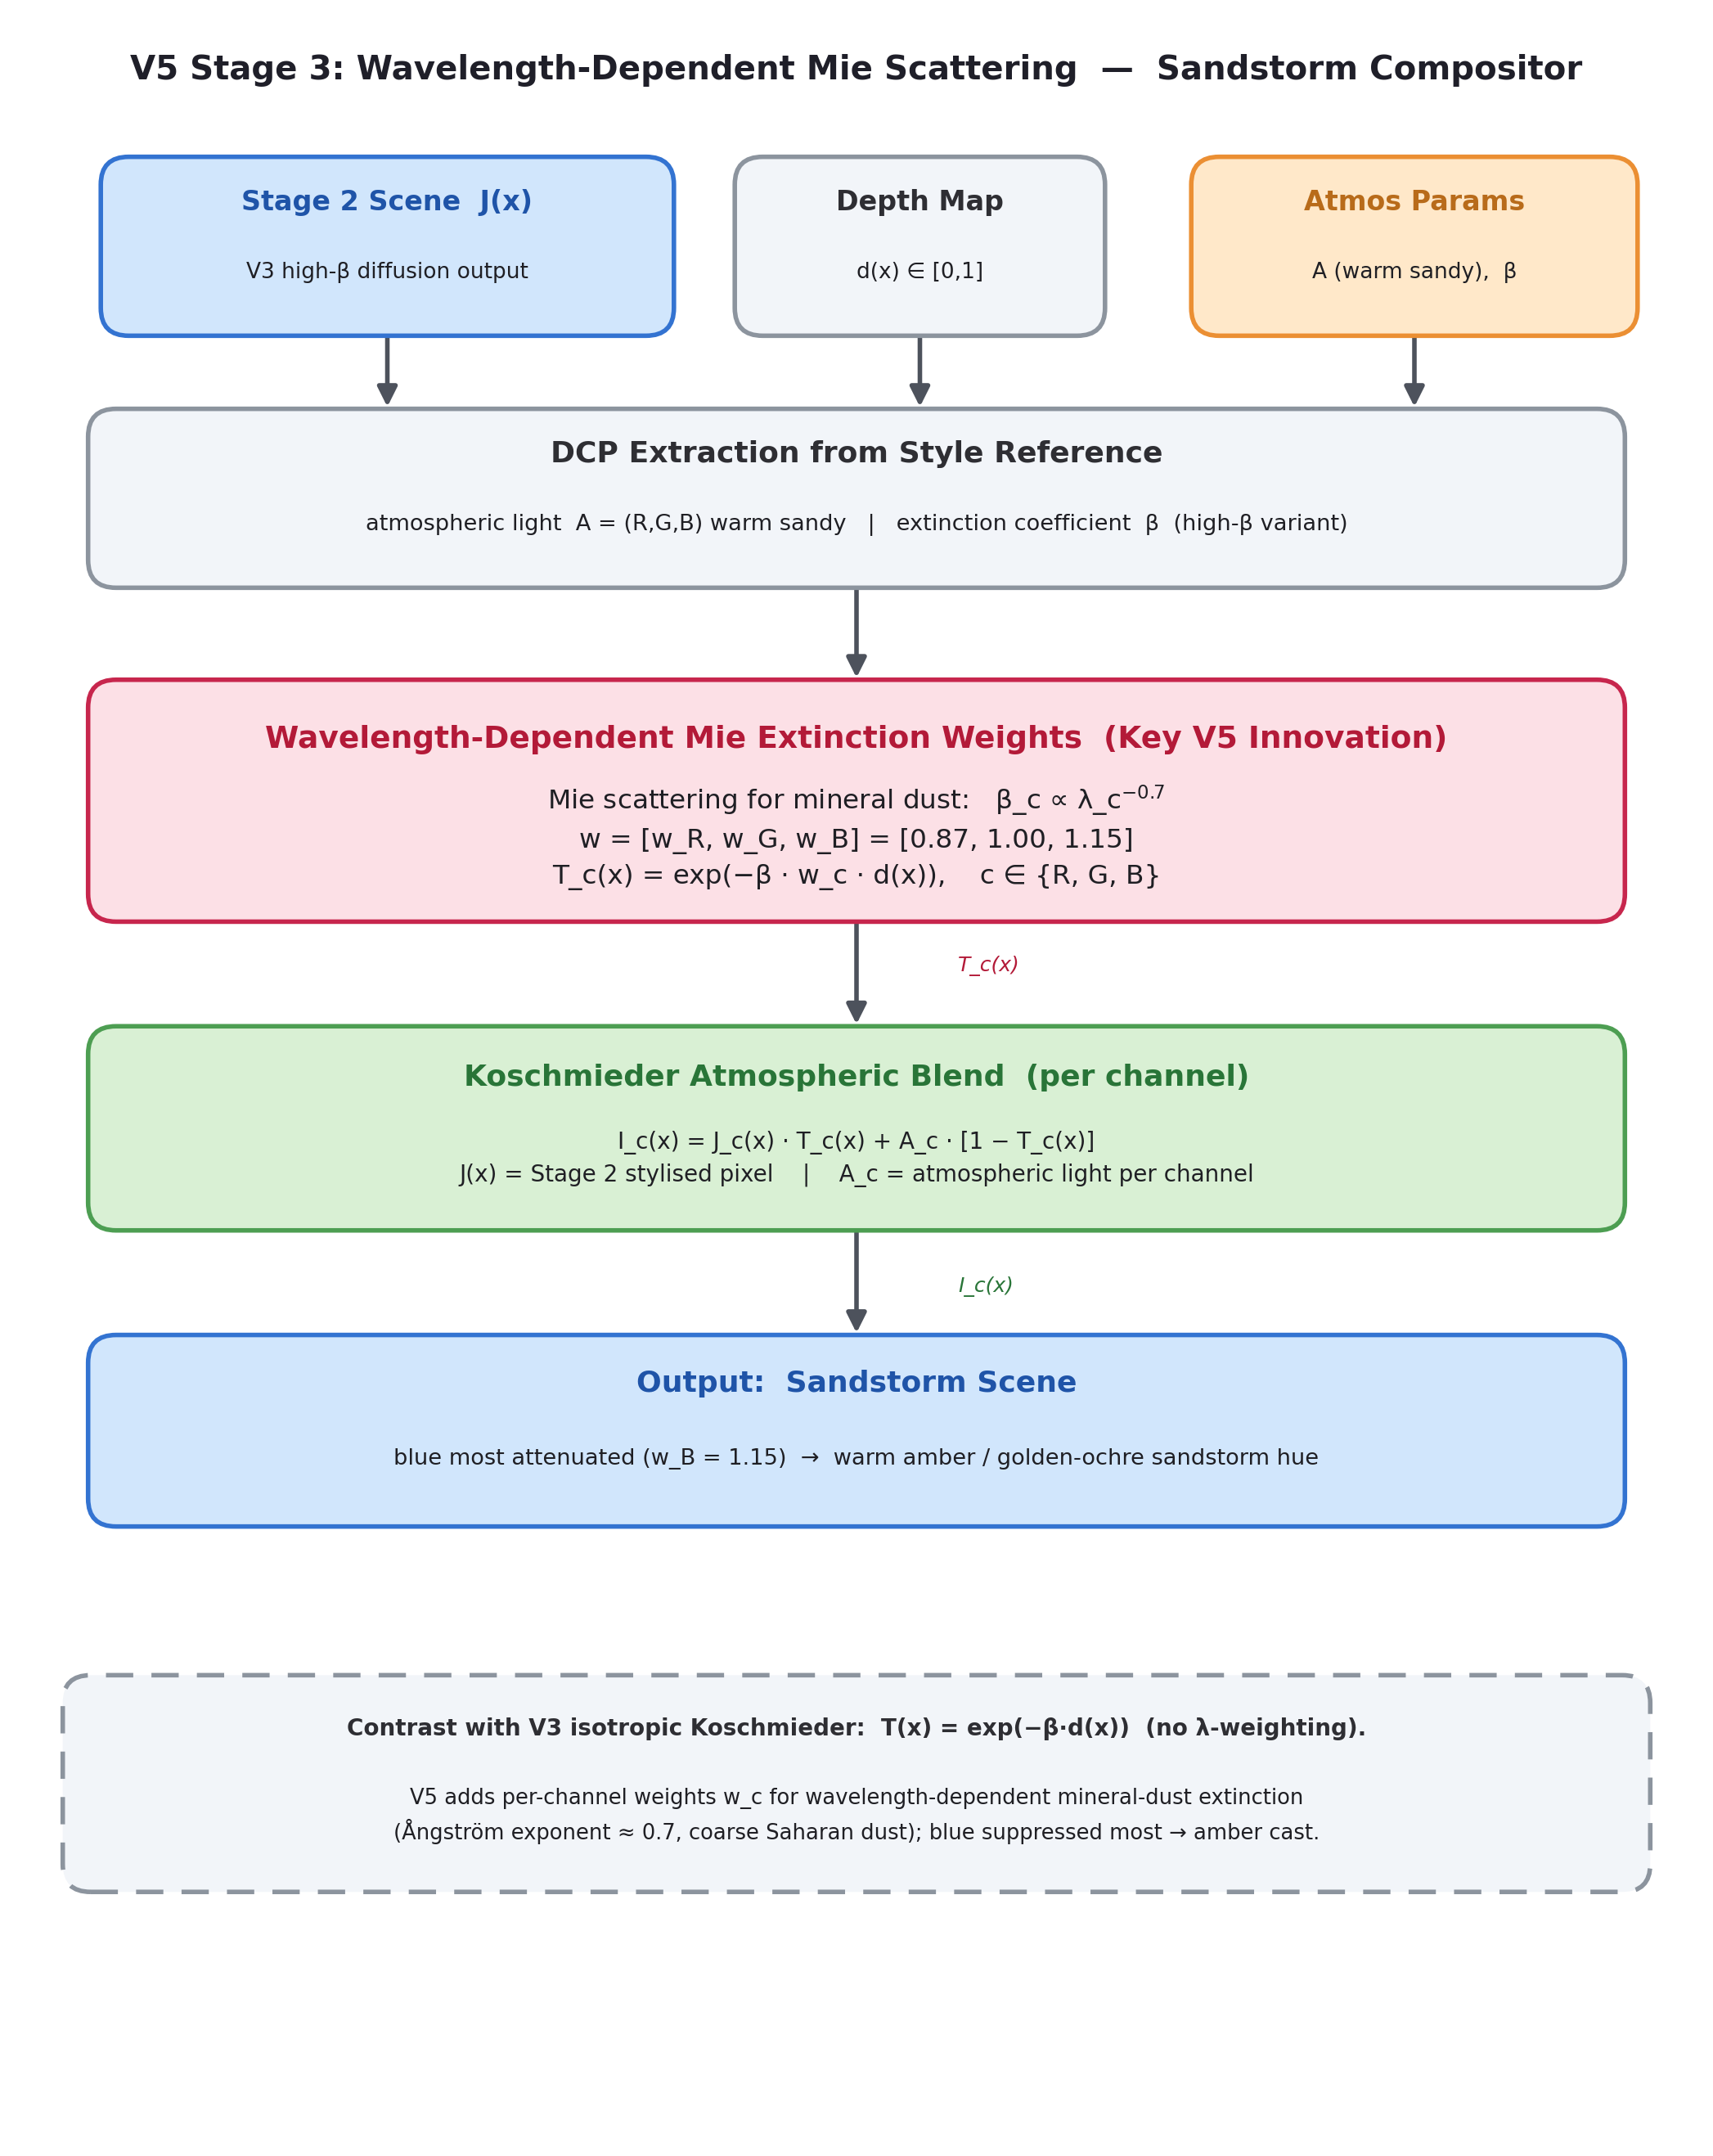
\includegraphics[width=0.82\linewidth]{images/arch_v5_stage3.png}
    \caption{V5 Stage~3 sandstorm compositor. The Stage~2 stylised scene, depth map, and DCP-extracted atmospheric parameters feed a wavelength-dependent Mie channel-weight block ($w_R{=}0.87$, $w_G{=}1.00$, $w_B{=}1.15$), yielding the warm amber sandstorm output. Per-channel equations are shown in the figure.}
    \label{fig:arch_v5_stage3}
\end{figure}

\begin{figure}[htbp]
    \centering
    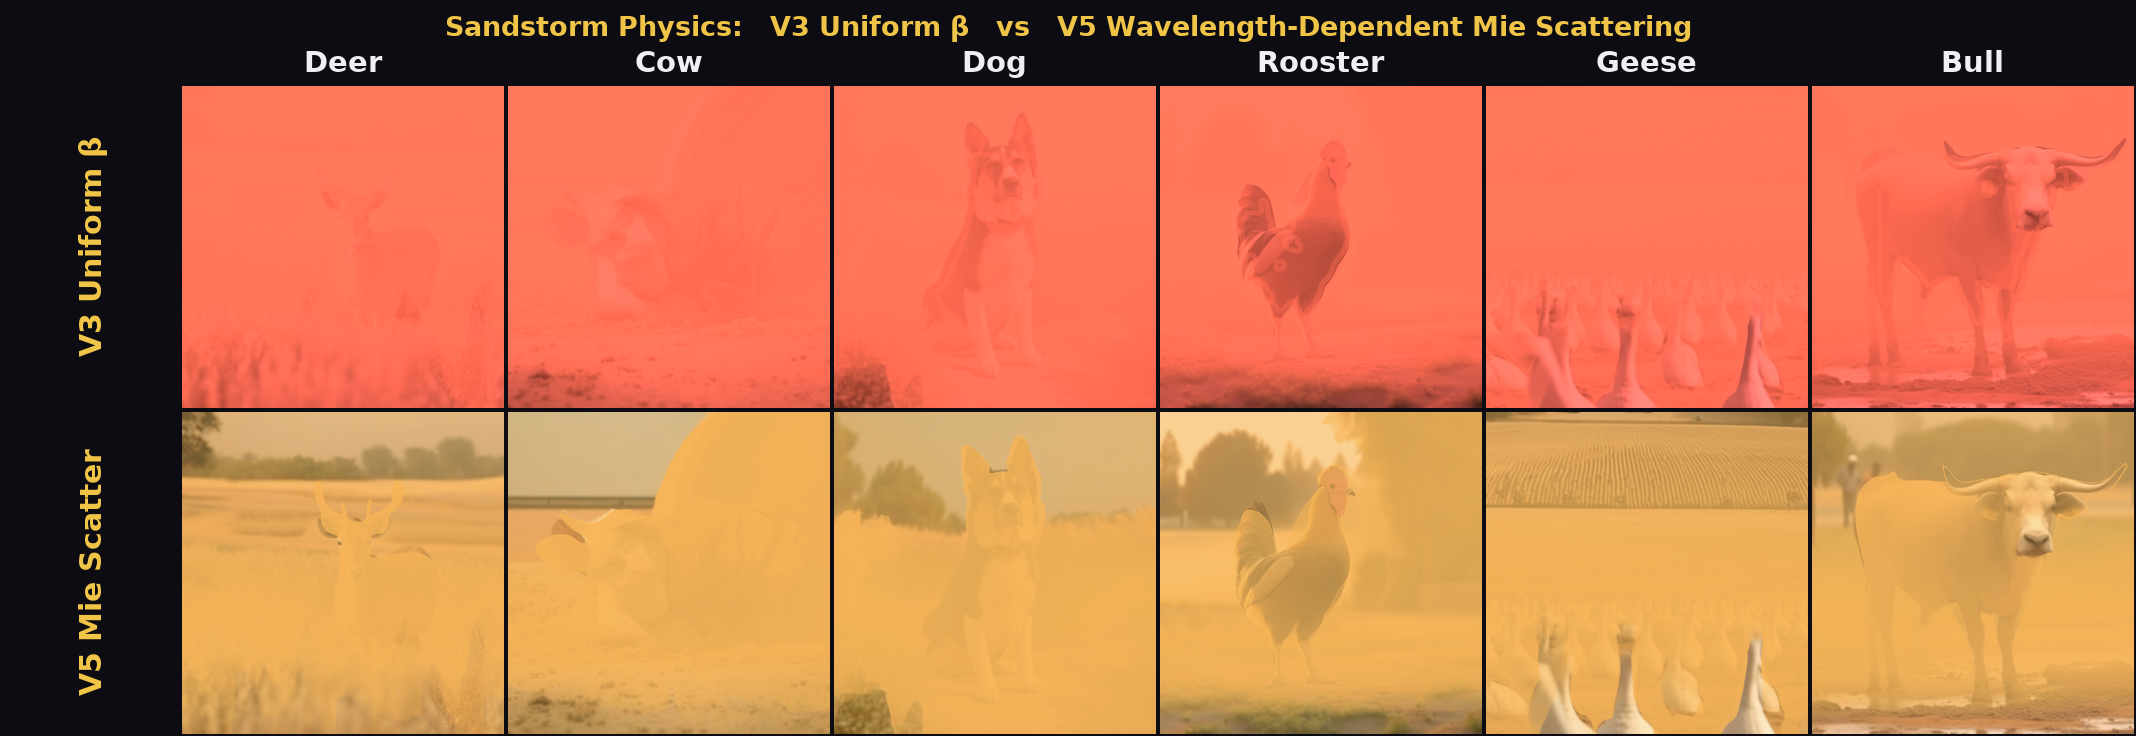
\includegraphics[width=0.96\linewidth]{images/v5_sandstorm.png}
    \caption{V3 uniform scattering vs.\ V5 wavelength-dependent Mie scattering applied to six content prompts (same sandstorm style reference). Channel-specific extinction coefficients ($\beta_B > \beta_G > \beta_R$) in V5 produce the characteristic warm amber colour shift of airborne mineral dust.}
    \label{fig:v5_sandstorm}
\end{figure}

\FloatBarrier
\subsection{V6: Procedural Snowfall Simulation}
\label{sec:v6_snowfall}

\noindent The key difference between snowstorms and fog or haze is that atmospheric particles are directly visible in the image. Individual snowflakes contribute to image formation and must be modelled separately from the volumetric scattering.

\noindent V6~(Table~\ref{tab:version_naming}) introduced a procedural snowfall layer computed after atmospheric compositing. Snow particles were generated using a depth-aware simulation where particle size, opacity, and blur radius vary according to estimated scene depth: larger particles appear closer to the camera; smaller, denser particles fill the far regions. Let $S(x)$ denote the synthesised snowfall layer. It is blended with the atmospheric image as:
\begin{equation}
    I_{\text{snow}}(x) = (1 - \alpha)\,I(x) + \alpha\,S(x),
\end{equation}
where $\alpha$ controls the snowfall intensity.

\noindent The visual result of V6~(Table~\ref{tab:version_naming}) snowfall is shown as the middle row of Figure~\ref{fig:v7_snow} alongside V3 and V7~(Table~\ref{tab:version_naming}) for direct comparison.

\FloatBarrier
\subsection{V7: Snow Accumulation Modelling}
\label{sec:v7_accumulation}

\noindent Although V6~(Table~\ref{tab:version_naming}) successfully generated snow particles, the images still lacked one of the most visually recognisable characteristics of snow environments: surface accumulation. Snow collects on horizontal surfaces — rooftops, farm equipment, fences, and ground regions — and this changes scene appearance in a way that cannot be replicated by atmospheric scattering or precipitation simulation alone.

\noindent V7~(Table~\ref{tab:version_naming}) applies three sequential stages to produce a physically complete winter scene.

\textbf{Stage 1 — Koschmieder base.} The standard depth-dependent compositor is applied with a cold white atmospheric light $A_{\text{snow}} = [0.92,\,0.94,\,0.98]$, causing distant objects to fade toward a blue-grey winter sky.

\textbf{Stage 2 — Surface accumulation.} A Sobel gradient computed on the DPT-Large depth map identifies locally flat regions. Surfaces with low gradient magnitude (flat), high nearness ($1-d(x)$), and upward-facing orientation (vertical weight) are assigned high accumulation probability. The accumulation mask $\alpha_g(x)$ is:
\begin{equation}
    \alpha_g(x) = \text{flatness}(x)\;\times\;\text{nearness}(x)\;\times\;\text{vertical\_weight}(x)\;\times\;\alpha_{\max},
\end{equation}
with $\alpha_{\max} = 0.70$. The accumulated image is then:
\begin{equation}
    I_a(x) = I_k(x)\,(1-\alpha_g(x)) + 255\cdot\alpha_g(x),
\end{equation}
where $I_k$ is the Koschmieder-composited image and the constant 255 represents the white snow colour.

\textbf{Stage 3 — Precipitation overlay.} Random snowflakes are placed at depth-weighted positions. Each flake has radius $r \in [1,\,4]$\,px and opacity $\alpha \in [0.25,\,0.90]$, both determined by nearness: foreground flakes are larger and more opaque; background flakes are smaller and translucent. The particle density is $\rho = 0.0008$ flakes per pixel. Let $M(x)$ denote the combined accumulation mask applied via Stage 2; the final output after all three stages is:
\begin{equation}
    I_{\text{accum}}(x) = (1 - M(x))\,I_{\text{snow}}(x) + M(x)\,C_{\text{snow}},
\end{equation}
where $I_{\text{snow}}$ includes the Stage 3 precipitation layer and $C_{\text{snow}}$ is the white snow colour. Only near, flat, and upward-facing surfaces accumulate snow; object boundaries and scene structure are preserved.

\begin{figure}[htbp]
    \centering
    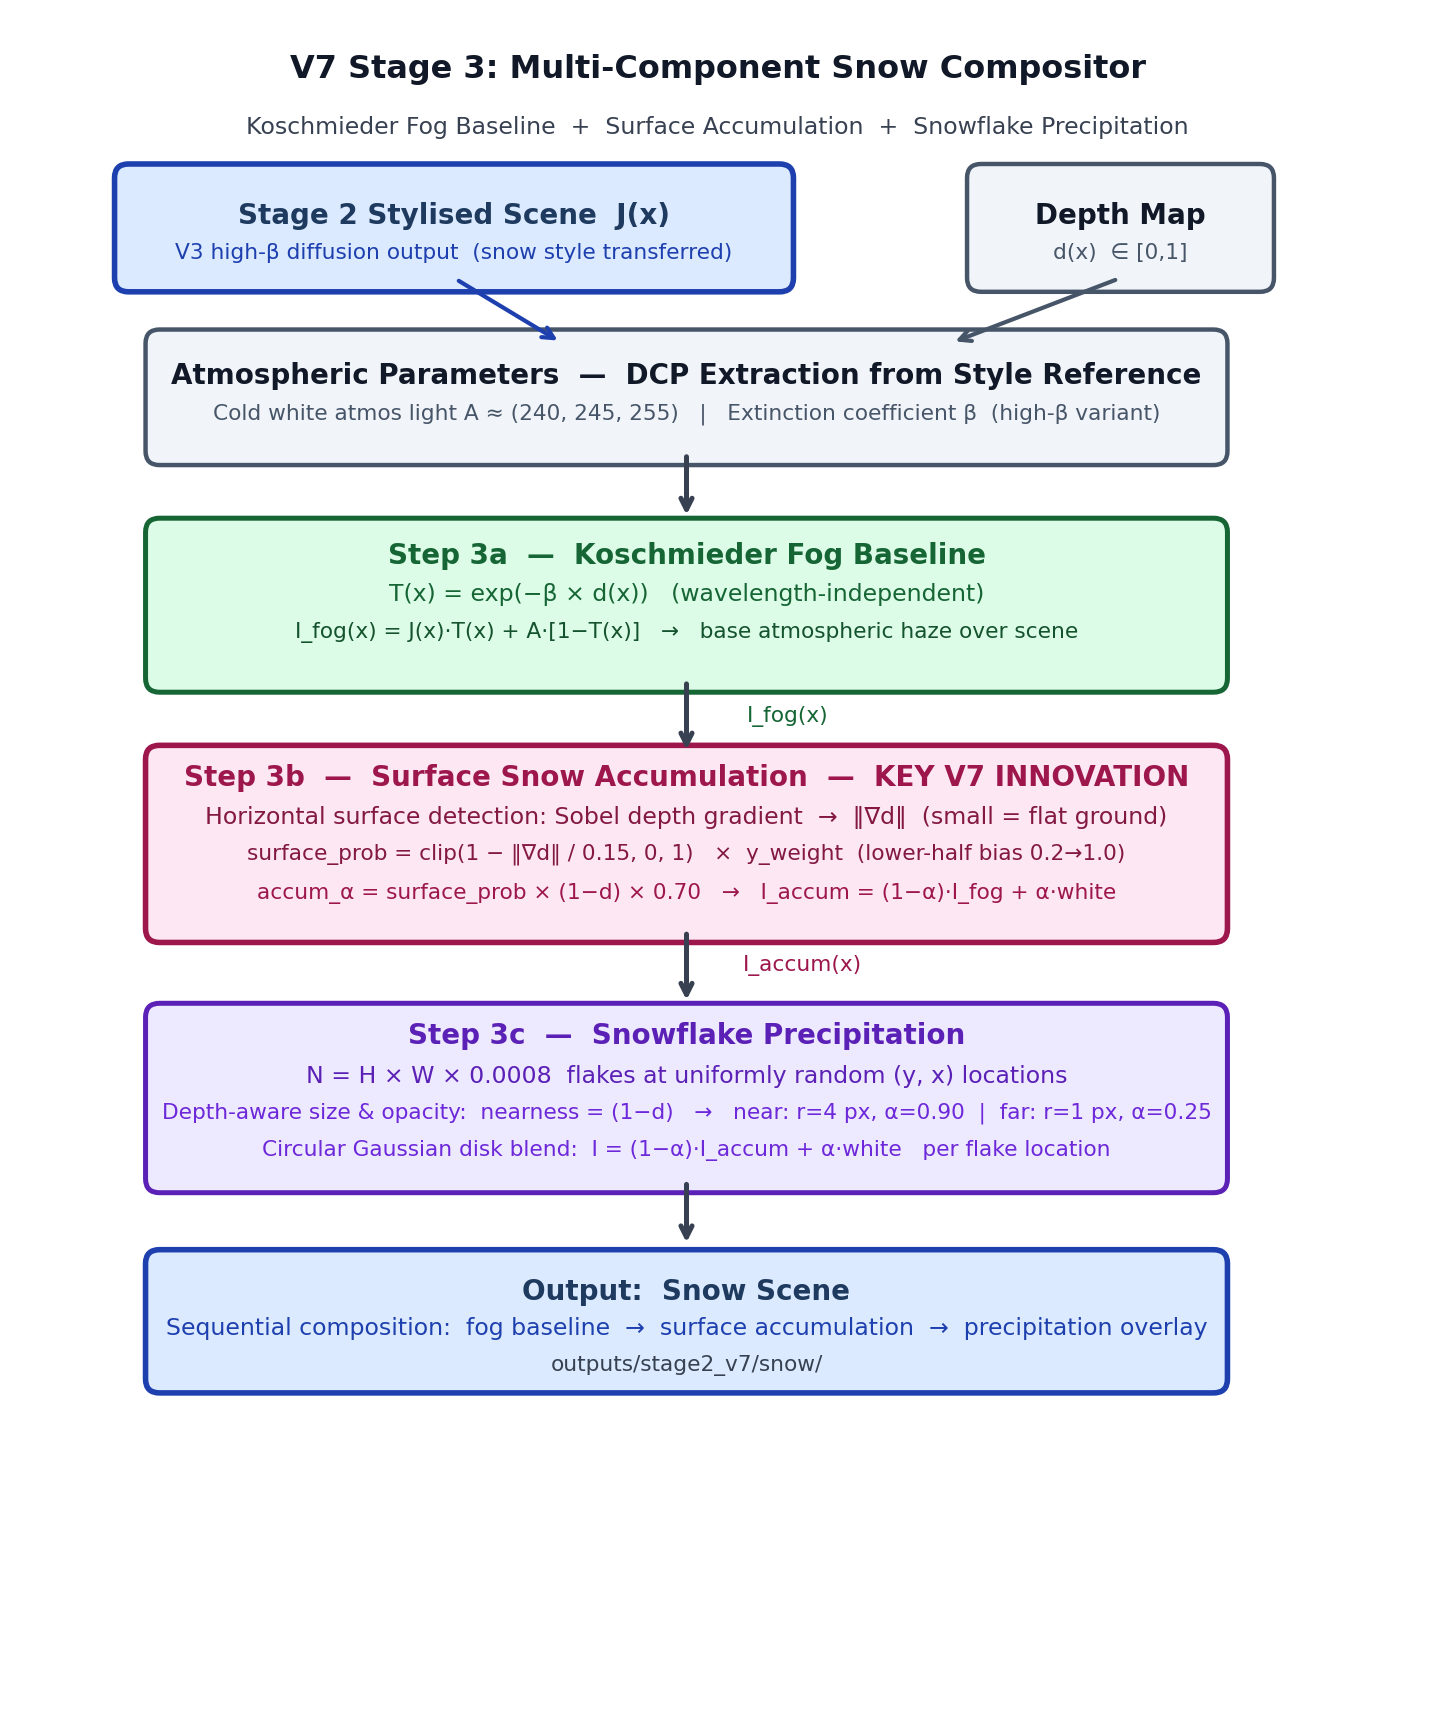
\includegraphics[width=0.82\linewidth]{images/arch_v7_stage3.png}
    \caption{V7 Stage~3 snow compositor architecture. The Stage~2 stylised scene and depth map feed through three sequential steps: \textbf{Step~3a} applies the standard Koschmieder fog baseline with cold white atmospheric light; \textbf{Step~3b} detects horizontal surfaces via Sobel depth gradients and overlays a white accumulation layer weighted by surface probability and nearness (max.\ opacity 0.70); \textbf{Step~3c} places $N = H \times W \times 0.0008$ snowflakes with depth-aware radius ($1$--$4$\,px) and opacity ($0.25$--$0.90$). The sequential composition produces a physically complete winter scene.}
    \label{fig:arch_v7_stage3}
\end{figure}

\begin{figure}[htbp]
    \centering
    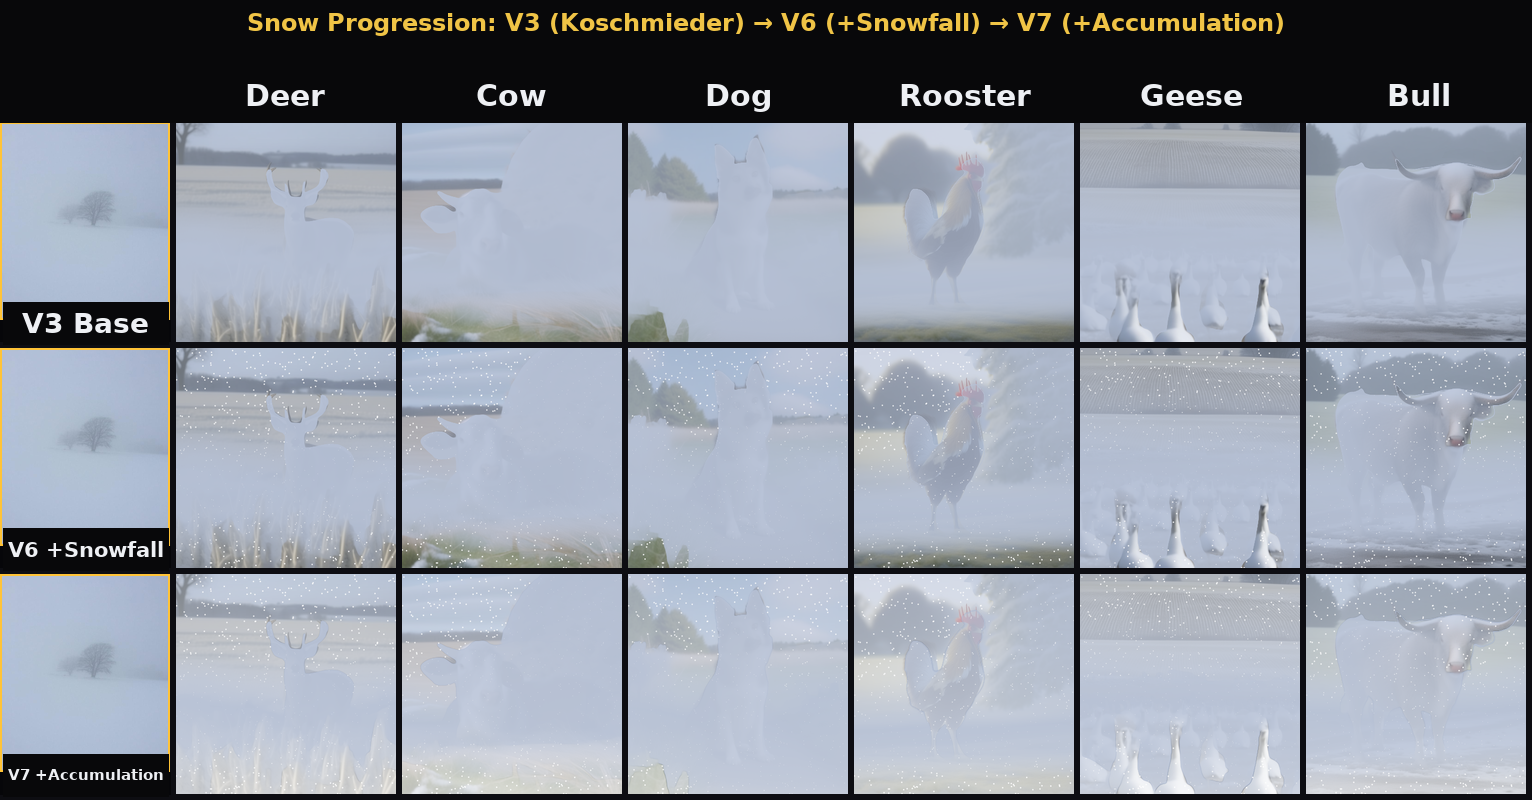
\includegraphics[width=0.96\linewidth]{images/v7_snow.png}
    \caption{Snow synthesis progression. V3~(top) applies Koschmieder visibility reduction; V6~(centre) adds depth-aware precipitation particles; V7~(bottom) further adds surface accumulation on plausible horizontal surfaces. V7 is the most physically complete winter model.}
    \label{fig:v7_snow}
\end{figure}

\begin{table}[htbp]
\centering
\caption{Summary of weather-specific physics refinements (V5--V7).}
\label{tab:physics_refinements}
\renewcommand{\arraystretch}{1.3}
\begin{tabular}{llp{7.5cm}}
\toprule
\textbf{Version} & \textbf{Focus} & \textbf{Core Contribution} \\
\midrule
V5 & Sandstorm Physics & Channel-specific Mie scattering ($\beta_B > \beta_G > \beta_R$) producing warm colour shift \\
V6 & Snowfall Simulation & Depth-aware procedural particle layer; foreground flakes larger than background \\
V7 & Snow Accumulation & Surface deposition mask from depth gradients; accumulation on horizontal surfaces \\
\bottomrule
\end{tabular}
\end{table}

\FloatBarrier
% -------------------------------------------------------
\section{V9: Content-Aware Atmospheric Style Transfer via Zero-Shot CLIP Embedding Subtraction}
\label{sec:v9}

\noindent V9~(Table~\ref{tab:version_naming}) addresses a fundamental limitation that persists across all prior configurations: \emph{content leakage from style reference images}. The style reference photographs used in Stages~V1--V3 are real-world atmospheric scenes that contain both the desired weather appearance (atmospheric texture, colour cast, visibility loss) and incidental semantic content (vegetation, ground plane, sky region, structures). The CLIP image encoder used by IP-Adapter captures both components simultaneously: the resulting image embedding is not a pure atmospheric descriptor but a superposition of atmospheric appearance and scene semantics. When this mixed embedding is injected into the SDXL generation process via IP-Adapter cross-attention, the content component contaminates the generated output — the synthesised scene inherits layout biases, vegetation density, and spatial arrangements from the style reference rather than from the content prompt.

\paragraph{Shared Embedding Space}
V9~(Table~\ref{tab:version_naming}) exploits a structural property of the SDXL and IP-Adapter architectures: the IP-Adapter image encoder (\texttt{CLIP ViT-bigG/14}) and the SDXL second text encoder (\texttt{text\_encoder\_2}) are initialised from the same \texttt{ViT-bigG/14} checkpoint and operate in the same 1280-dimensional embedding space. This co-residency is not coincidental — SDXL's dual-encoder design was specifically constructed so that the image-level CLIP representations and text-level CLIP representations are comparable within a shared geometric space~\cite{podell2023sdxlimprovinglatentdiffusion}. This property makes direct linear operations (summation, subtraction, interpolation) between image embeddings and text embeddings geometrically valid: the two modalities share the same basis directions, so subtracting a text direction from an image embedding removes the component of the image that aligns with the named concept.

\paragraph{Zero-Shot Content Identification}
The dominant semantic content of each style reference image is identified without any manual annotation. A candidate set $\mathcal{C}$ of 22 natural-language phrases is defined, covering common atmospheric scene subjects (persons, animals, vehicles, terrain, infrastructure). For a given style reference image $\mathbf{s}$, the dominant content label $c^*$ is determined by:
\begin{equation}
    c^* = \operatorname*{argmax}_{c \in \mathcal{C}} \; \cos\!\bigl(\phi_I(\mathbf{s}),\, \phi_T(c)\bigr),
    \label{eq:content_detection}
\end{equation}
where $\phi_I(\cdot)$ is the CLIP image encoder and $\phi_T(\cdot)$ is the CLIP text encoder. The candidate phrases include categories such as ``a person'', ``a tree'', ``farmland'', ``a road'', ``a mountain'', ``a building'', and additional domain-relevant terms. The highest-scoring candidate identifies the primary semantic object present in the style reference, requiring no labelled data or human supervision.

\paragraph{Content Subtraction in Embedding Space}
Given the detected content label $c^*$ and the original style reference embedding $\mathbf{e}_I = \phi_I(\mathbf{s})$, the content component is removed by projecting out the text direction $\mathbf{e}_T = \phi_T(c^*)$:
\begin{equation}
    \tilde{\mathbf{e}}_I = \mathrm{normalize}\!\Bigl(\hat{\mathbf{e}}_I - \alpha \cdot \hat{\mathbf{e}}_T\Bigr) \cdot \|\mathbf{e}_I\|,
    \label{eq:content_subtraction}
\end{equation}
where $\hat{\mathbf{e}}_I = \mathbf{e}_I / \|\mathbf{e}_I\|$ and $\hat{\mathbf{e}}_T = \mathbf{e}_T / \|\mathbf{e}_T\|$ are unit-normalised embeddings, $\alpha = 0.45$ is the subtraction strength, and the result is rescaled by the original norm $\|\mathbf{e}_I\|$ to preserve the magnitude expected by the IP-Adapter. The subtracted embedding $\tilde{\mathbf{e}}_I$ is used in place of $\mathbf{e}_I$ as the image prompt throughout Stage~2.

\noindent The operation in Equation~\ref{eq:content_subtraction} can be interpreted geometrically: the unit-normalised style embedding $\hat{\mathbf{e}}_I$ is shifted by $-\alpha \hat{\mathbf{e}}_T$ in the direction that would be activated by the concept $c^*$, followed by renormalisation to the unit hypersphere. The re-scaling by $\|\mathbf{e}_I\|$ preserves the injection intensity in IP-Adapter's cross-attention layers. This is analogous to concept vector arithmetic in distributed word embedding spaces, here applied to multimodal image–language embeddings.

\paragraph{Block Configuration and Inference Hyperparameters}
V9 adopts an extended block-selective injection scheme that includes the \texttt{mid\_block} in addition to the \texttt{up\_blocks.0} and \texttt{up\_blocks.1} blocks used in V3. The \texttt{mid\_block} operates at the bottleneck of the UNet and captures the highest-level structural features; including it improves low-frequency colour and luminance alignment with the atmospheric reference without the layout-leakage pathology of full all-block injection observed in V1. The IP-Adapter injection scale is set to 0.95 throughout. Unlike V3, V9 re-enables CSD guidance ($\eta=0.25$, $w_\mathrm{CSD}=1.5$, applied every 3 denoising steps using the raw style reference image $\mathbf{s}$); at the lower denoising strengths of pure t2i generation, CSD does not produce the destructive interference observed in V4 and instead provides complementary perceptual anchoring.

\begin{table}[htbp]
\centering
\caption{V9 configuration parameters.}
\label{tab:v9_config}
\begin{tabular}{ll}
\toprule
\textbf{Parameter} & \textbf{Value} \\
\midrule
Content detection candidates $|\mathcal{C}|$ & 23 \\
Content subtraction strength $\alpha$ & 0.45 \\
IP-Adapter injection blocks & \texttt{up\_blocks.0}, \texttt{up\_blocks.1}, \texttt{mid\_block} \\
IP-Adapter injection scale & 0.95 \\
Generation mode & Pure t2i (no img2img) \\
Denoising steps & 50 \\
Guidance scale & 7.5 \\
CSD guidance $\eta$ / weight / interval & 0.25 / 1.5 / every 3 steps \\
Style references per domain & 3 (haze, sandstorm, snow) \\
Random seeds per configuration & 3 \\
Stage~3 physics: haze & Koschmieder scattering (V3), $\beta_\mathrm{scale}=1.2$ \\
Stage~3 physics: sandstorm & Mie per-channel scattering (V5), $\mathbf{w}=[0.87,\,1.00,\,1.15]$ \\
Stage~3 physics: snow & Snowflake particles + surface accumulation (V7) \\
\bottomrule
\end{tabular}
\end{table}

\begin{figure}[htbp]
    \centering
    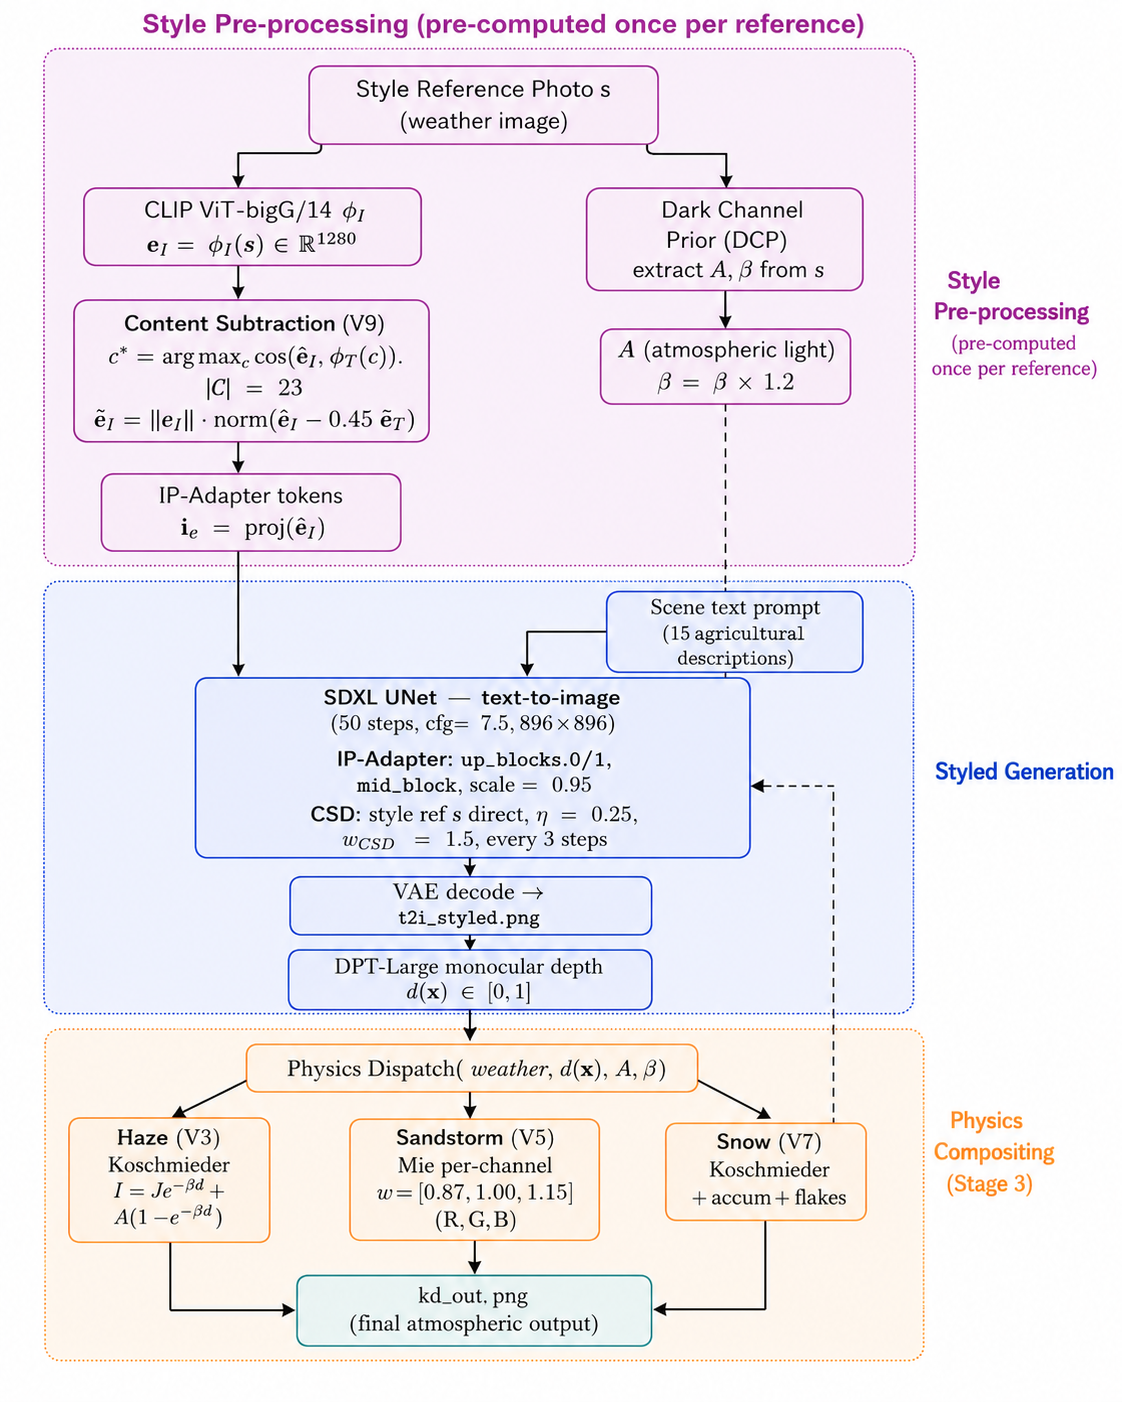
\includegraphics[width=0.95\linewidth, height=0.74\textheight, keepaspectratio]{images/v9_arch.png}
    \caption{V9 pipeline architecture. \textbf{Violet:} The style reference $\mathbf{s}$ is encoded by CLIP ViT-bigG/14; zero-shot content detection over 23 labels identifies $c^*$ whose text direction is subtracted ($\alpha=0.45$) to produce atmospheric-only IP tokens $\mathbf{ie}$. DCP extracts atmospheric light $A$ and extinction $\beta$ ($\times1.2$). \textbf{Blue:} Scene text prompt and $\mathbf{ie}$ drive SDXL t2i with block-selective IP-Adapter (\texttt{up$_0$/up$_1$/mid}, scale$=0.95$) and CSD ($\eta=0.25$, $w=1.5$, every 3 steps). \textbf{Orange:} DPT-Large depth and DCP-derived $A,\beta$ feed weather-specific physics: haze~(V3 Koschmieder), sandstorm~(V5 Mie per-channel), snow~(V7 + accumulation + snowflakes).}
    \label{fig:arch_v9_stage2}
\end{figure}

\paragraph{Weather-Specific Physics Dispatch}
The Stage~3 compositor in V9 dispatches to three physics backends depending on the atmospheric domain, rather than the single Koschmieder compositor used in V3:

\begin{itemize}
    \item \textbf{Haze}: Standard Koschmieder scattering (Equation~\ref{eq:koschmieder}) with scattering coefficients boosted by a scale factor $\beta_\mathrm{scale} = 1.2$ relative to DCP-estimated values, to produce denser and more visually challenging haze. Atmospheric light $A$ is estimated per-image from the style reference.
    \item \textbf{Sandstorm}: Mie scattering with per-channel attenuation weights $\mathbf{w} = [0.87,\, 1.00,\, 1.15]$ for the RGB channels respectively, reflecting the wavelength-dependent scattering of coarse mineral particulates under Mie theory (longer wavelengths scatter less, producing the characteristic warm amber-yellow tonal shift of sandstorm imagery).
    \item \textbf{Snow}: A two-component compositor comprising (i) simulated snowflake particle overlays (Gaussian blobs with randomised spatial placement at flake density $\rho_\mathrm{flake} = 8 \times 10^{-4}$ per pixel) and (ii) a surface accumulation layer applied to horizontal flat regions, with maximum accumulation opacity $\alpha_\mathrm{accum} = 0.70$.
\end{itemize}

\paragraph{Experimental Scale}
V9 was evaluated across 15 scene prompts $\times$ 9 style references (3 per atmospheric domain) $\times$ 3 random seeds, producing 405 images in total across the three atmospheric conditions. The complete set of 405 images was successfully generated, representing the final and most extensible configuration produced during this research.

\paragraph{Design Rationale and Limitations}
The fundamental design rationale of V9 is the separation of \emph{what the atmosphere looks like} (captured by the IP-Adapter style embedding) from \emph{what scene content is incidentally present} in the style reference (identified by zero-shot CLIP classification and removed by embedding subtraction). This disentanglement allows the generator to receive a more spectrally pure atmospheric signal during IP-Adapter injection. The approach requires no additional training, no labelled style reference annotations, and no modifications to the SDXL or IP-Adapter weights; the entire operation is performed at inference time on the pre-computed CLIP embeddings.

\noindent A practical limitation is that the subtraction strength $\alpha$ is a fixed scalar applied uniformly across all candidate–reference pairs. In style references where the dominant semantic content has a large projection onto the atmospheric signal (e.g., a hazy scene dominated by a single large tree that also provides the colour cast), setting $\alpha$ too high can inadvertently suppress genuine atmospheric components. The value $\alpha = 0.45$ was selected as a conservative balance point: sufficient to attenuate content interference without eliminating atmospheric colour and texture information.

\begin{figure}[H]
    \centering
    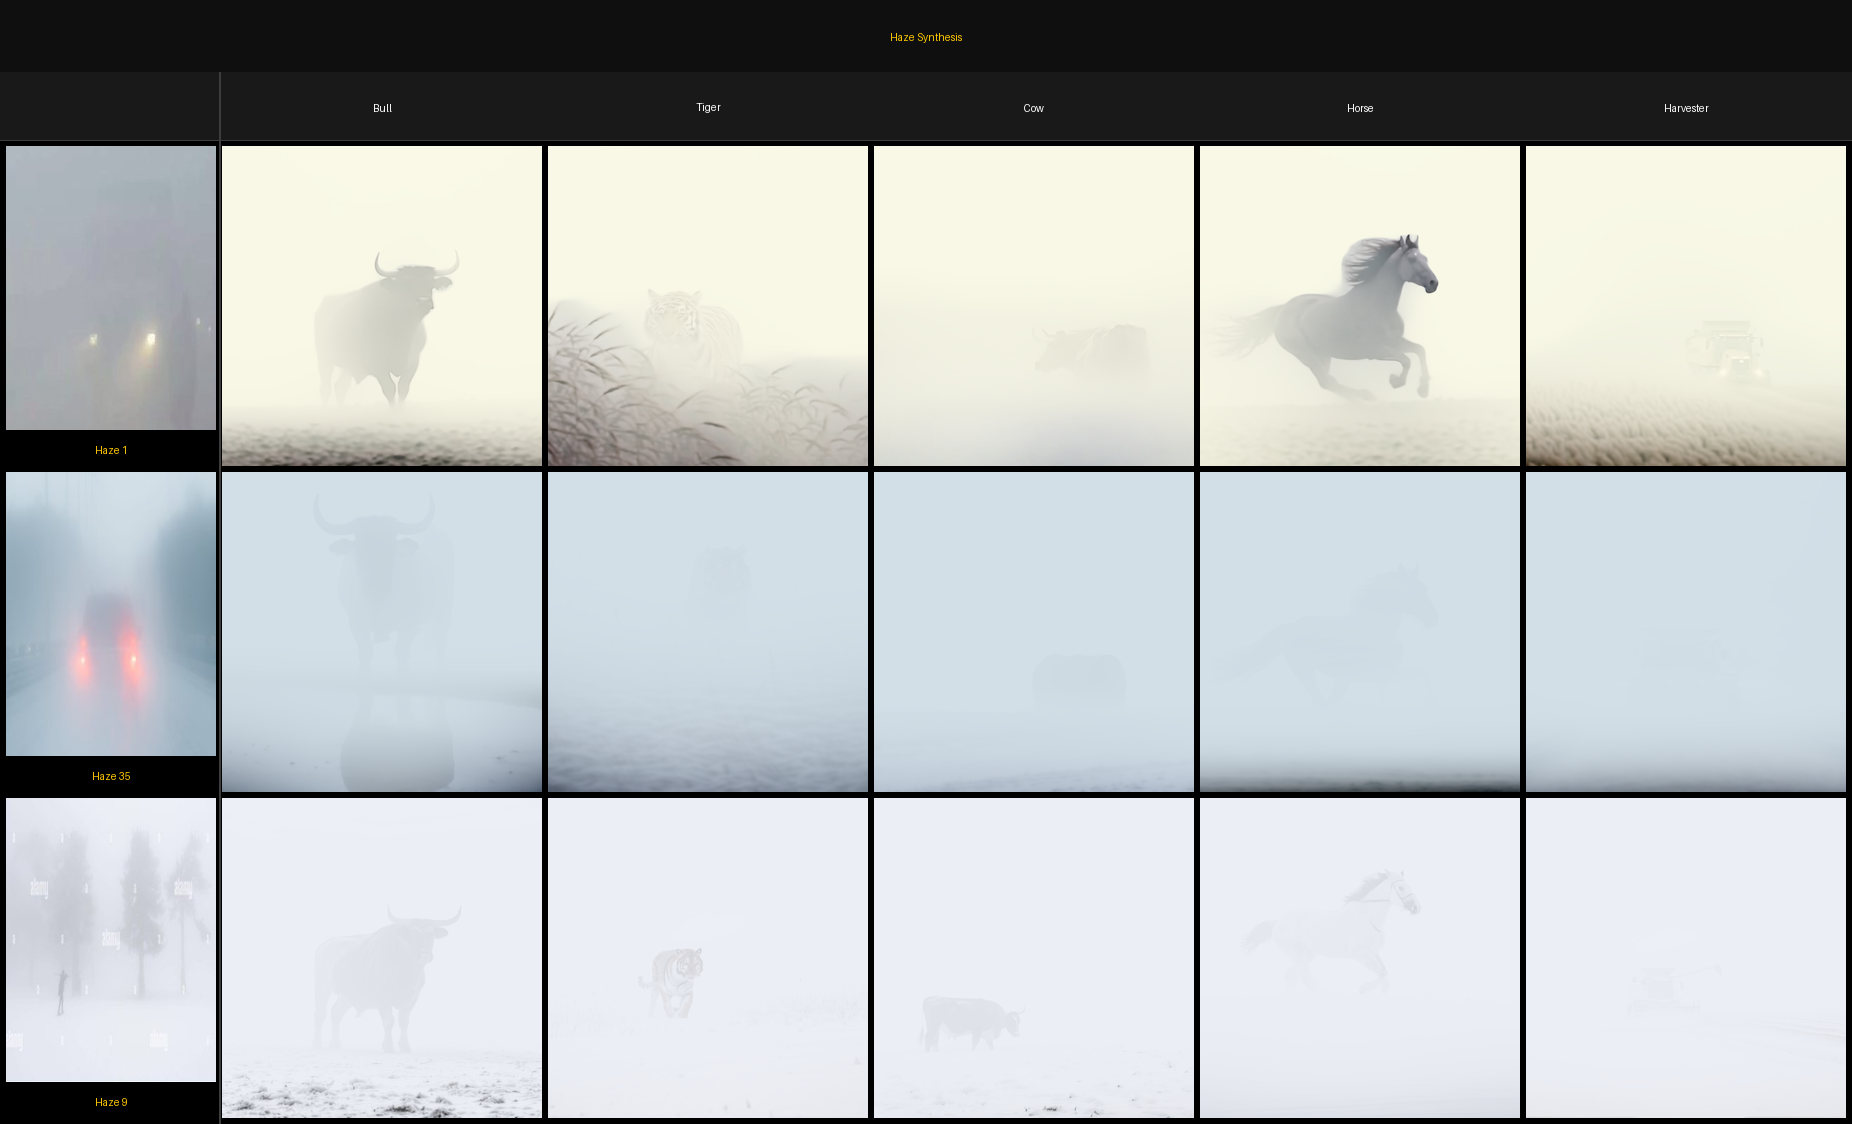
\includegraphics[width=0.96\linewidth]{images/haze_synthesis_v9.png}
    \caption{V9 haze synthesis results: three style references (rows) across five content subjects --- Bull, Tiger, Cow, Horse, and Harvester (columns). Each image is conditioned via CLIP content-subtraction ($\alpha = 0.45$) followed by Koschmieder physics compositing.}
    \label{fig:v9_haze_results}
\end{figure}

\begin{figure}[H]
    \centering
    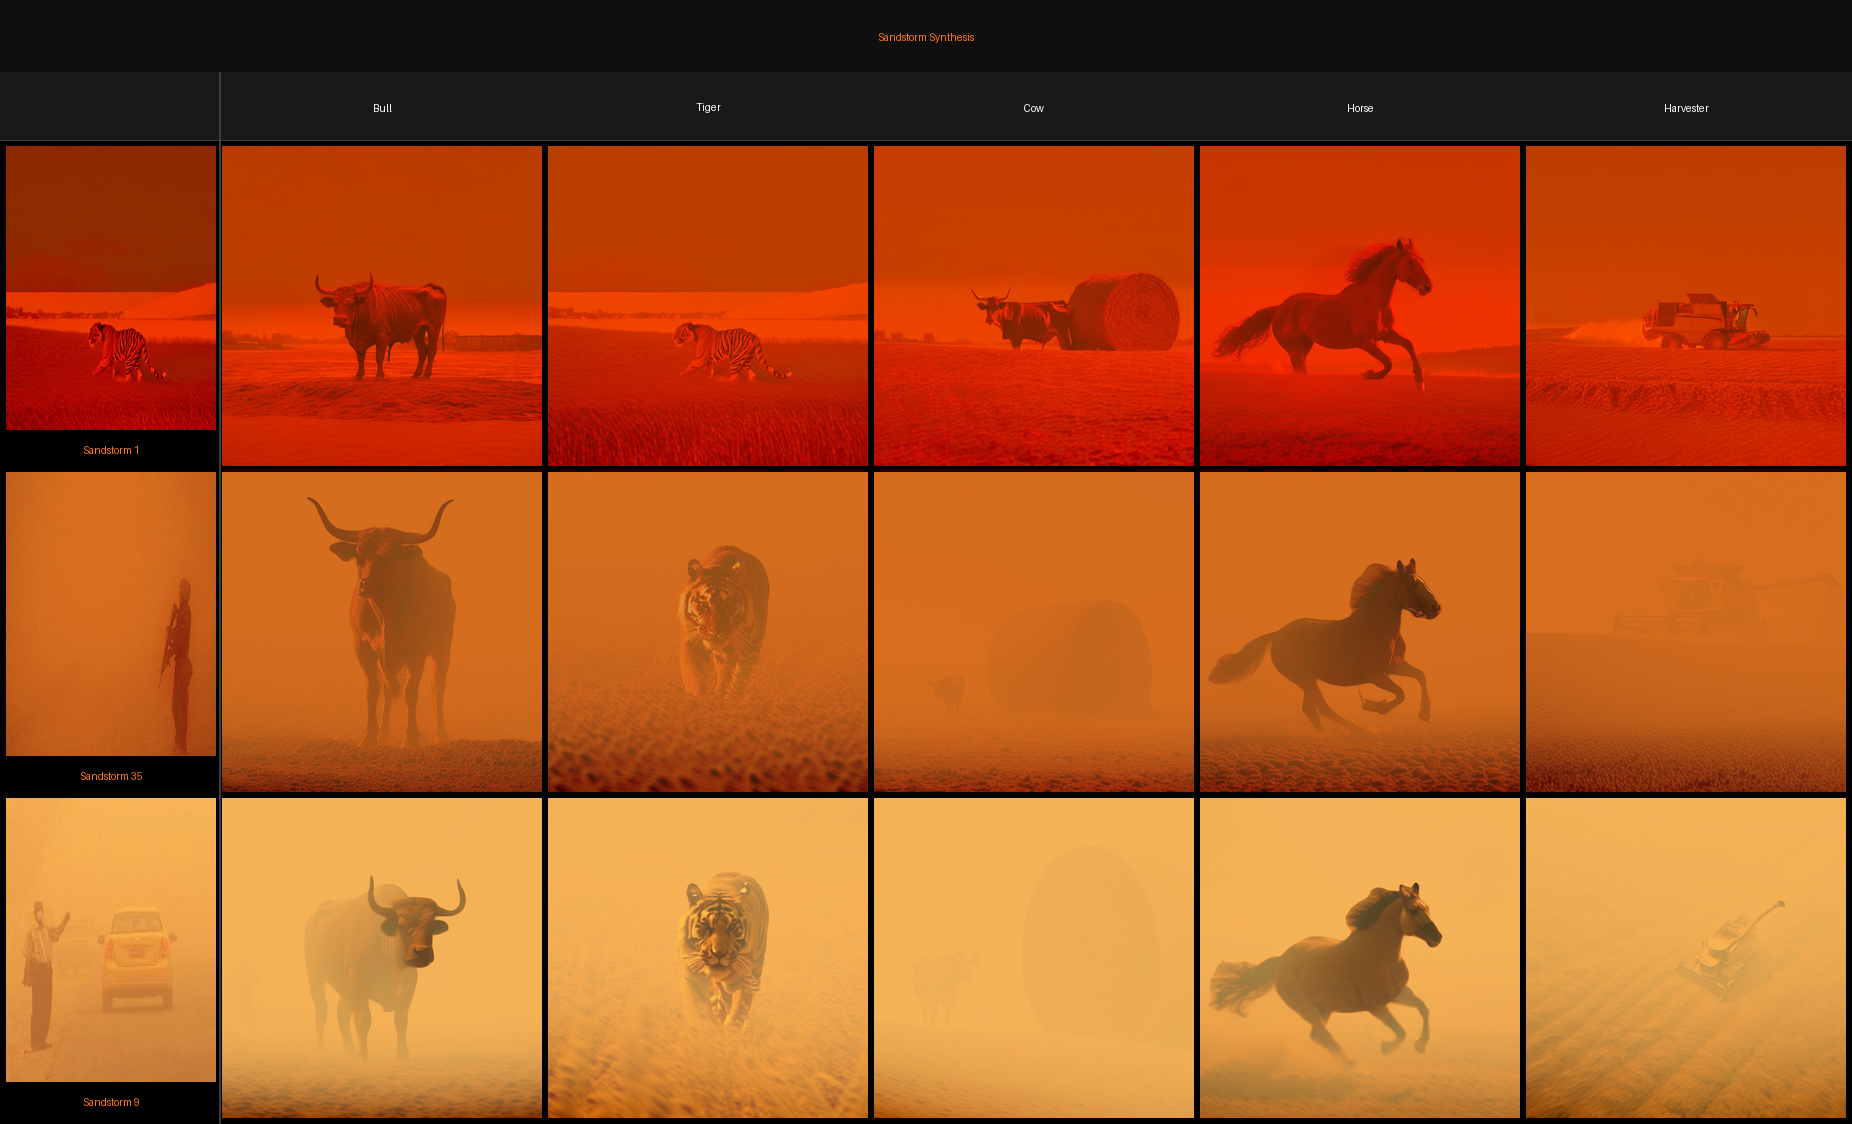
\includegraphics[width=0.96\linewidth]{images/sandstorm_synthesis_v9.png}
    \caption{V9 sandstorm synthesis results: three warm amber sand-dust style references (rows) across five content subjects (columns). Mie per-channel scattering ($\mathbf{w} = [0.87, 1.00, 1.15]$) in Stage~3 produces the characteristic warm amber tonal shift.}
    \label{fig:v9_sandstorm_results}
\end{figure}

\begin{figure}[H]
    \centering
    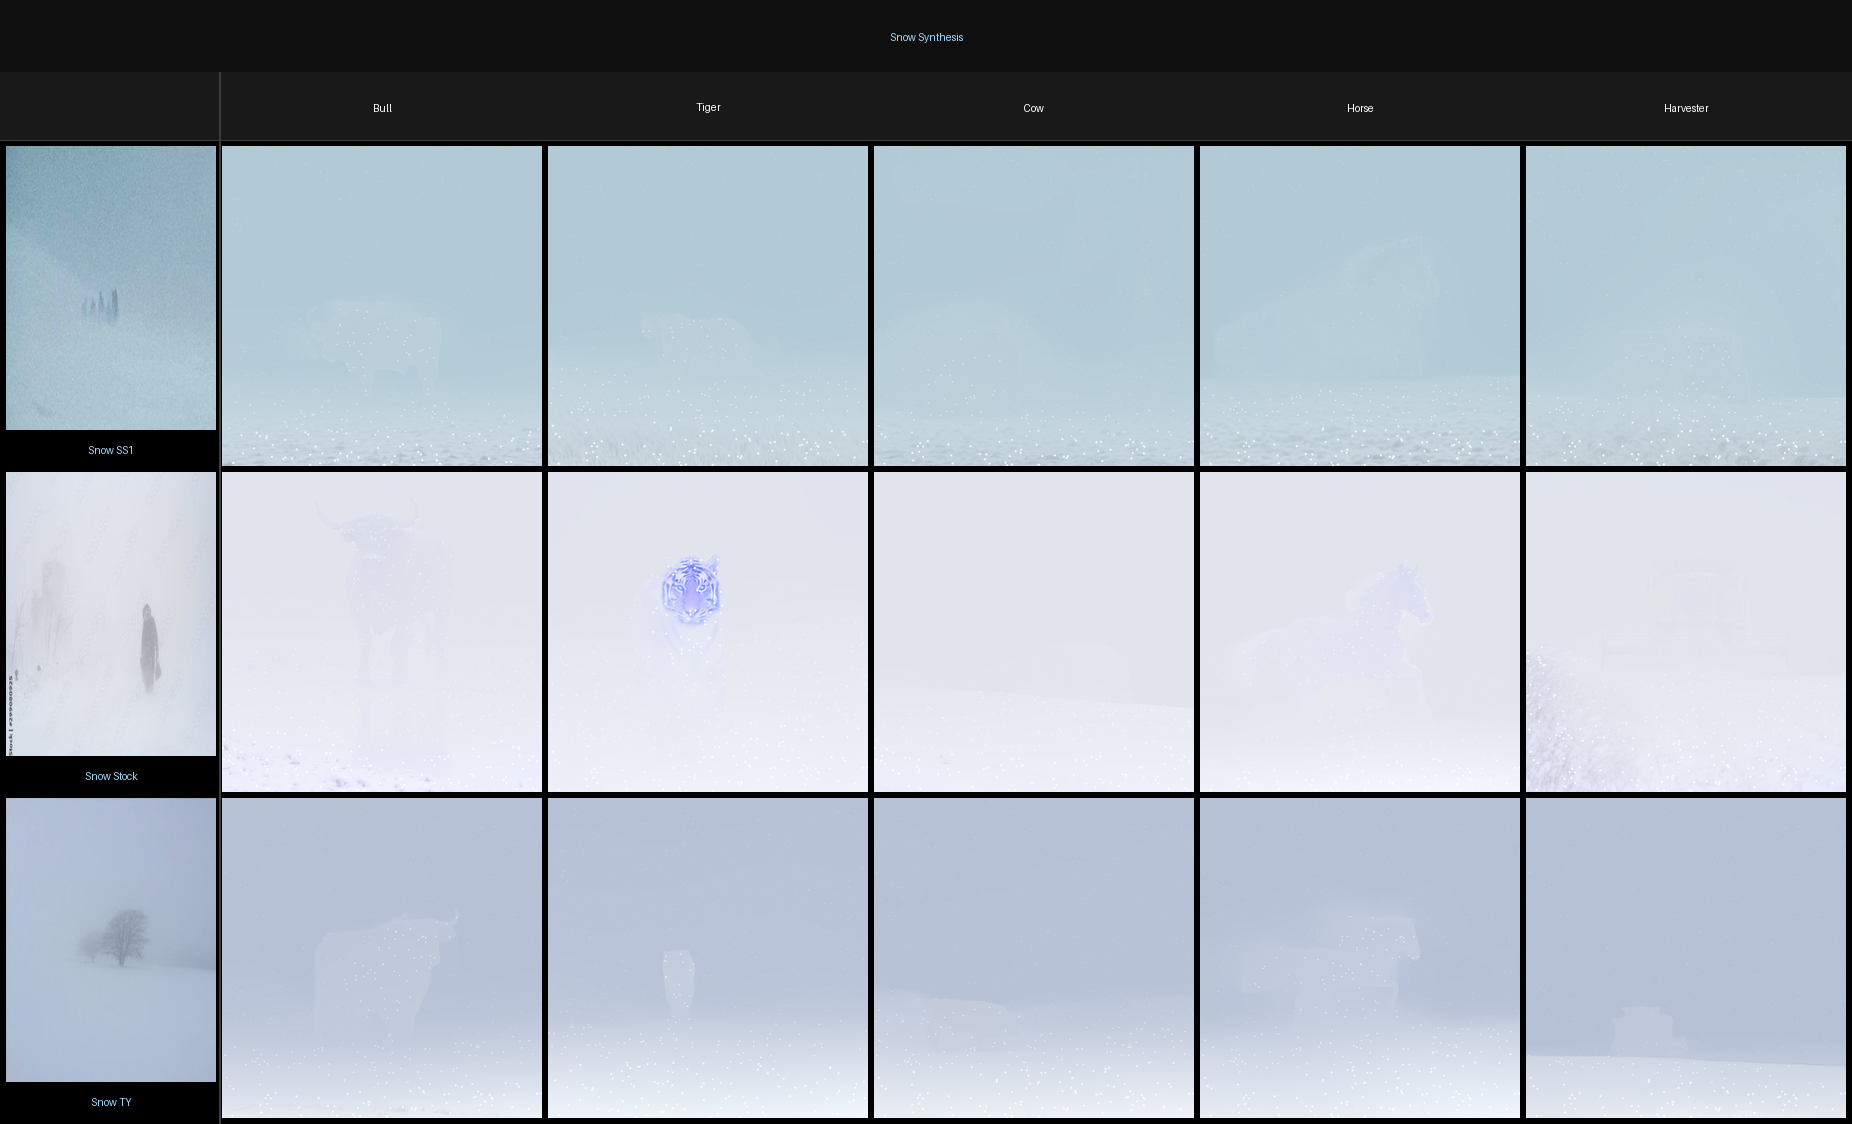
\includegraphics[width=0.96\linewidth]{images/snow_synthesis_v9.png}
    \caption{V9 snow synthesis results: three cold-weather style references (rows) across five content subjects --- Tiger, Deer, Dog, Boar, and Donkey (columns). Stage~3 adds snowflake particles and surface accumulation to achieve realistic winter scene compositing.}
    \label{fig:v9_snow_results}
\end{figure}

\FloatBarrier
% =====================================================
\section{Downstream Experiments}
\label{sec:phase2_experiments}

\noindent Five experiments were conducted using the synthesized atmospheric dataset to measure its utility for training vision models.

\paragraph{A Note on Metric Comparability with the Style Transfer Study}
Before presenting results, one potential source of confusion must be addressed. The style transfer study reported top-1 accuracy of \textbf{76.4\%} on style-transferred outputs while V3 of the proposed pipeline reports \textbf{67.2\%} on its outputs --- at first glance the proposed pipeline appears weaker on this metric. It is not.

The difference is entirely due to the classifier used. The most direct cross-method comparison uses a single metric: CLIP ViT-L-14 average max-softmax confidence. Lower confidence means the model is more uncertain about what class it is looking at, indicating stronger distributional shift. Table~\ref{tab:cross_phase_clip} shows the result.

\begin{table}[htbp]
\centering
\caption{Cross-method comparison on a unified metric: CLIP avg max-softmax confidence (lower = stronger domain shift = more physically realistic). All style transfer methods evaluated on the same agricultural content prompts used in the proposed pipeline (60 images per method, 4 atmospheric style references). Physics pipeline numbers from Experiment~1. Both ViT-L-14 and ViT-H-14 (metaclip\_fullcc) reported.}
\label{tab:cross_phase_clip}
\renewcommand{\arraystretch}{1.3}
\resizebox{\textwidth}{!}{%
\begin{tabular}{llcc}
\toprule
\textbf{Stage} & \textbf{Method / Split} & \textbf{ViT-L-14 Conf.\ ($\downarrow$)} & \textbf{ViT-H-14 Conf.\ ($\downarrow$)} \\
\midrule
Baseline          & Clean CIFAR-10              & 0.341 & 0.335 \\
\midrule
Style Transfer    & InstantStyle (baseline)     & 0.661 & 0.652 \\
Style Transfer    & InstantStyle-Plus           & 0.698 & 0.659 \\
Style Transfer    & StyleShot                   & 0.620 & 0.552 \\
Style Transfer    & CSGO                        & 0.625 & 0.587 \\
Style Transfer    & V0 (CSD-Guided Latent Optimisation) & 0.514 & 0.438 \\
\midrule
Physics Pipeline  & V2 (Block-Selective + CSD)                      & 0.316 & 0.303 \\
Physics Pipeline  & V3 (Physics-Grounded Atmospheric Compositing)   & 0.274 & 0.246 \\
Physics Pipeline  & V9 (Semantic-Decoupled Atmospheric Style Transfer) & \textbf{0.228} & \textbf{0.227} \\
\bottomrule
\end{tabular}}
\par\smallskip
{\footnotesize\noindent
V0 (IS+CSD Guidance) achieves the lowest confidence among all style transfer methods (0.514 / 0.438) but remains above the clean baseline (0.341 / 0.335) on both encoders. All physics pipeline methods fall below the clean baseline. \textbf{V9 achieves the lowest overall confidence (0.228 / 0.227) of any method evaluated}, representing the strongest domain shift.}
\end{table}

\noindent A controlled re-evaluation on the same 15 agricultural prompts and 4 atmospheric style references reveals a clear three-level hierarchy. The four passive style transfer baselines (InstantStyle, InstantStyle-Plus, StyleShot, CSGO) yield CLIP ViT-L-14 confidence between 0.620 and 0.698 --- well above both the ViT-L-14 clean baseline (0.341) and the ViT-H-14 clean baseline (0.335), indicating that passive style injection does not substantially confuse modern vision encoders. V0~(Table~\ref{tab:version_naming}) (InstantStyle + CSD Guidance), with active latent correction, reduces confidence to 0.514 (L-14) and 0.438 (H-14) --- the lowest of any style transfer method --- yet both values remain above the clean baseline (0.341 / 0.335), confirming that appearance-based style injection cannot cross this threshold regardless of guidance sophistication. V3 at 0.274 (L-14) / 0.246 (H-14) falls below both clean baselines, and \textbf{V9 achieves the strongest domain shift of all evaluated methods (0.228 / 0.227)}, demonstrating that zero-shot CLIP content subtraction combined with physics compositing produces a fundamentally deeper distributional shift than anything achievable with learned style transfer alone.

% -------------------------------------------------------
\FloatBarrier
\subsection{Experiment 1: Pipeline Comparison (V3 vs V9)}
\label{sec:exp1}

\noindent \textbf{Goal:} Determine whether V9's zero-shot CLIP content subtraction and extended block injection produce a stronger feature-space domain shift than the V3 baseline across all three atmospheric conditions.

\noindent \textbf{Data.} Both pipelines produce 405 images each (15 prompts $\times$ 9 style references $\times$ 3 seeds, across haze, sandstorm, and snow). The same ViT-L-14 and ViT-H-14 (metaclip\_fullcc) encoders are used throughout, with mean max cosine-softmax confidence over a 100-class ImageNet vocabulary as the primary metric.

\begin{table}[htbp]
\centering
\caption{Experiment~1: Zero-shot confidence and Top-1 accuracy on V3 and V9 pipeline outputs. Lower confidence = stronger domain shift. Per-weather breakdown shows where each pipeline's atmospheric effect is strongest.}
\label{tab:exp1_pipeline_comparison}
\renewcommand{\arraystretch}{1.3}
\resizebox{\textwidth}{!}{%
\begin{tabular}{llcccc}
\toprule
\textbf{Pipeline} & \textbf{Weather} & \multicolumn{2}{c}{\textbf{ZS Confidence ($\downarrow$)}} & \multicolumn{2}{c}{\textbf{Top-1 Accuracy ($\downarrow$)}} \\
\cmidrule(lr){3-4}\cmidrule(lr){5-6}
& & \textbf{ViT-L-14} & \textbf{ViT-H-14} & \textbf{ViT-L-14 (\%)} & \textbf{ViT-H-14 (\%)} \\
\midrule
Clean scenes & All & 0.339 & 0.334 & — & — \\
\midrule
\multirow{4}{*}{V3} & Haze       & \textbf{0.219} & \textbf{0.220} & 60.7 & 60.7 \\
                    & Sandstorm  & 0.302          & 0.266          & 68.9 & 68.2 \\
                    & Snow       & 0.289          & 0.267          & 70.4 & 73.3 \\
                    & \textit{All} & 0.270        & 0.249          & 68.4 & 67.2 \\
\midrule
\multirow{4}{*}{V9} & Haze       & 0.231          & 0.244          & 62.2 & 61.5 \\
                    & Sandstorm  & 0.281          & 0.261          & 78.5 & 80.0 \\
                    & Snow       & \textbf{0.171} & \textbf{0.180} & \textbf{41.5} & \textbf{37.8} \\
                    & \textit{All} & \textbf{0.228} & \textbf{0.227} & \textbf{62.2} & \textbf{59.8} \\
\bottomrule
\end{tabular}}
\end{table}

\noindent V9 achieves the lowest overall confidence on both backbones (0.228 vs 0.270 for ViT-L-14; 0.227 vs 0.249 for ViT-H-14). The per-weather breakdown reveals a clear pattern: V3 haze is marginally stronger (0.219 vs 0.231), but V9 snow is dramatically more challenging — 0.171 ViT-L-14, the lowest single-condition score in the entire study. This is a direct consequence of V7~(Table~\ref{tab:version_naming})'s two-component snow compositor (surface accumulation + precipitation particles), which alters scene appearance more aggressively than any pure visibility-based model. V9 sandstorm also slightly outperforms V3 (0.281 vs 0.302), attributable to V5~(Table~\ref{tab:version_naming})'s wavelength-dependent Mie scattering preserving the warm colour cast at greater depth.

\noindent The corresponding Top-1 accuracy drop is most striking for snow: from 70.4\% (V3) to 41.5\% (V9) on ViT-L-14. This means that for nearly 60\% of V9 snow images, the pretrained ViT cannot confidently identify the correct agricultural scene class — confirming that the V9 snow model produces a qualitatively harder recognition problem than any prior pipeline version.

% -------------------------------------------------------
\FloatBarrier
\subsection{Experiment 2: Linear Probe Adaptation}
\label{sec:exp2}

\noindent \textbf{Goal:} Measure how much of the atmospheric domain gap can be closed by linear probing on frozen ViT features, and whether a probe trained on V3 data transfers to V9 images — and vice versa.

\noindent \textbf{Setup.} Two separate linear probes are trained: one on V3 highbeta (405 images, 80/20 split) and one on V9 (405 images, 80/20 split). Both use \texttt{LogisticRegression} on L2-normalised CLIP image features with no backbone fine-tuning. Cross-distribution evaluation tests whether the V3-trained probe transfers to V9 images without retraining.

\begin{table}[htbp]
\centering
\caption{Experiment~2: Zero-shot vs linear probe accuracy across evaluation sets. V3 and V9 probes work in-distribution but do not cross-transfer, confirming that each physics pipeline creates a distinct feature-space distribution.}
\label{tab:exp2_linear_probe}
\renewcommand{\arraystretch}{1.3}
\resizebox{\textwidth}{!}{%
\begin{tabular}{llccc}
\toprule
\textbf{Backbone} & \textbf{Eval Set} & \textbf{Zero-Shot} & \textbf{Linear Probe} & \textbf{Gain} \\
\midrule
\multirow{4}{*}{ViT-L-14}
  & V3 test split (in-dist)        & 79.0\% & 86.4\% (V3 probe)  & +7.4 pp \\
  & Extreme haze ($\beta=9.0$)     & 82.2\% & 93.3\% (V3 probe)  & +11.1 pp \\
  & V9 test split (in-dist)        & 66.7\% & 76.5\% (V9 probe)  & +9.8 pp \\
  & V9 images (V3 probe xfer)      & 65.9\% & 65.4\% (V3 probe)  & $-$0.5 pp \\
\midrule
\multirow{4}{*}{ViT-H-14}
  & V3 test split (in-dist)        & 77.8\% & 87.7\% (V3 probe)  & +9.9 pp \\
  & Extreme haze ($\beta=9.0$)     & 86.7\% & 93.3\% (V3 probe)  & +6.6 pp \\
  & V9 test split (in-dist)        & 65.4\% & 71.6\% (V9 probe)  & +6.2 pp \\
  & V9 images (V3 probe xfer)      & 65.7\% & 60.2\% (V3 probe)  & $-$5.5 pp \\
\bottomrule
\end{tabular}}
\end{table}

\noindent Two findings stand out. First, both probes produce meaningful in-distribution gains: the V3 probe achieves +7.4 pp (ViT-L-14) on V3 test data, and the V9 probe achieves +9.8 pp on V9 test data. The V3 probe also generalises well to extreme synthetic haze ($\beta = 9.0$, 3$\times$ normal density), confirming that the probe has learned to handle atmospheric degradation within the same physics regime.

\noindent Second, \textbf{cross-distribution transfer completely fails}: the V3-trained probe applied to V9 images yields $-$0.5 pp and $-$5.5 pp relative to zero-shot on ViT-L-14 and ViT-H-14 respectively — essentially no improvement or a regression. This is a direct consequence of V9's CLIP content subtraction and extended block injection fundamentally altering the feature-space distribution relative to V3. A probe adapted to V3's IP-Adapter style transfer characteristics does not transfer to V9's content-subtracted embeddings, even though both datasets cover the same 15 scene classes. Each pipeline version requires its own domain adaptation.

% -------------------------------------------------------
\FloatBarrier
\subsection{Experiment 3: Probe Generalisation to Real Animal Photographs}
\label{sec:exp3}

\noindent \textbf{Goal:} Test whether probes trained entirely on \emph{synthetic} atmospheric images (V3 or V9) generalise to recognise \emph{real} animal photographs that they have never encountered during training.

\noindent \textbf{Data.} 57 real photographs from the \texttt{real\_object\_inference} collection. These are clear-weather images taken in natural conditions with no synthetic processing — a strict out-of-training-distribution test. They divide into two groups:
\begin{itemize}
    \item \textbf{In-distribution (N\,=\,34):} Eight animal categories overlapping with the V3/V9 training class set: tiger (5), deer (7), cow (6), horse (10), geese (3), boar (1), dog (1), donkey (1).
    \item \textbf{Out-of-distribution (N\,=\,23):} Twelve animal classes not present in training: bear, bison, camel, cheetah, crane bird, elephant, leopard, polar bear, rabbit, scarecrow, sheep, wolf.
\end{itemize}

\begin{table}[htbp]
\centering
\caption{Experiment~3: Zero-shot CLIP, V3 probe, and V9 probe evaluated on 57 real animal photographs. In-dist Top-1 measures recognition of known-class animals (N\,=\,34); OOD Max-Conf is the mean maximum predicted probability on animals never seen during training (N\,=\,23) --- lower indicates better calibration.}
\label{tab:exp3_real_photos}
\resizebox{\textwidth}{!}{%
\renewcommand{\arraystretch}{1.3}
\begin{tabular}{llccc}
\toprule
\textbf{Backbone} & \textbf{Method} & \textbf{In-dist Top-1 (\%)} & \textbf{In-dist Top-3 (\%)} & \textbf{OOD Max-Conf ($\downarrow$)} \\
\midrule
\multirow{3}{*}{ViT-L-14} & Zero-shot CLIP & 55.9          & 91.2          & 0.587 \\
                            & V3 probe       & \textbf{73.5} & 79.4          & \textbf{0.116} \\
                            & V9 probe       & 70.6          & \textbf{82.3} & \textbf{0.115} \\
\midrule
\multirow{3}{*}{ViT-H-14} & Zero-shot CLIP & 67.7          & 97.1          & 0.607 \\
                            & V3 probe       & \textbf{73.5} & 79.4          & \textbf{0.121} \\
                            & V9 probe       & 70.6          & \textbf{88.2} & \textbf{0.120} \\
\bottomrule
\end{tabular}
}
\end{table}

\paragraph{In-distribution accuracy.}
Both probes substantially outperform zero-shot on Top-1 recognition: the V3 probe achieves 73.5\% (ViT-L-14) compared to 55.9\% for zero-shot CLIP — a \textbf{+17.6 pp improvement} from a probe trained exclusively on synthetic atmospheric images. The V9 probe achieves 70.6\% (+14.7 pp). These gains are large enough to be practically meaningful: probes trained on generated data recognise real animals more reliably than a state-of-the-art zero-shot model with no atmospheric adaptation.

\noindent On Top-3 accuracy, the V9 probe achieves 82.3\% (ViT-L-14) and 88.2\% (ViT-H-14), surpassing the V3 probe's 79.4\%, suggesting that V9's harder training distribution expands the ranking of plausible classes even when Top-1 is slightly lower. The V3 probe's marginally higher Top-1 is consistent with V3's more naturalistic atmospheric synthesis: less aggressive degradation means the probe features align more closely with clear real photographs.

\paragraph{OOD calibration.}
The probe has no ability to \emph{identify} OOD animals — it outputs probabilities over only its 15 known farm-animal classes, none of which include bear, wolf, elephant, or the other 12 OOD species. What the OOD Max-Conf metric measures is therefore \emph{calibration}: when presented with an unseen animal, does the model confidently commit to an incorrect known class, or does it correctly spread probability and remain uncertain?

\noindent This is a non-trivial question. A wolf in CLIP feature space overlaps with ``dog in a field''; a bison overlaps with ``bull in a paddock''; a bear overlaps with ``wild boar in a field.'' A poorly calibrated model could plausibly assign 60--80\% confidence to these spurious matches. Zero-shot CLIP, evaluated over the same restricted 15-class softmax, achieves exactly this: 0.587 (ViT-L-14) and 0.607 (ViT-H-14) — it is 59--61\% confident in a wrong class assignment for OOD animals.

\noindent Both probes reduce this to 0.115--0.121: a \textbf{5$\times$ reduction in overconfident misclassification}. The atmospheric training constrains the probe's decision surface: the probe has learned that a correct classification requires not just visual similarity to a farm animal class but also the feature signature of atmospherically degraded training images. Clear-weather bear and wolf photographs do not carry this signature, so the probe correctly abstains. For deployment in drone-based agricultural monitoring, this matters practically — a probe that signals uncertainty on a novel species allows a safety fallback to activate, whereas a zero-shot model that outputs ``wild boar'' with 60\% confidence may suppress further inspection.

% -------------------------------------------------------
\FloatBarrier
\subsection{Experiment 4: Real-World Domain Transfer Validation}
\label{sec:exp4}

\noindent \textbf{Goal:} Validate that V3 adaptation transfers to real-world atmospheric photographs from independent benchmark collections — confirming that the synthetic pipeline captures properties of real atmospheric degradation rather than diffusion-model generation artefacts.

\noindent \textbf{Setup.} 145 real atmospheric photographs were used: 57 haze images, 58 sandstorm images, and 30 snow images drawn from curated real-world atmospheric datasets. These images carry no agricultural GT class labels, so classification accuracy cannot be measured directly. Calibration is instead assessed via \emph{mean max-confidence}: the mean maximum predicted probability across the 15-class output for a given backbone and method.

\noindent A correctly domain-adapted model should produce a physically consistent confidence hierarchy: highest on clean images (high visual quality, unambiguous content), intermediate on synthetic V3 atmospheric images (the trained distribution), and lowest on real-world atmospheric images (genuinely degraded, most challenging). Table~\ref{tab:exp4_calibration_hierarchy} reports this three-regime comparison.

\begin{table}[htbp]
\centering
\caption{Experiment~4: Mean max-confidence of zero-shot CLIP vs V3-adapted linear probe across three data regimes and per weather domain. Lower confidence on atmospheric images reflects correct domain-awareness. The probe maintains the physically expected ordering (clean $>$ synthetic $>$ real-world) on both backbones.}
\label{tab:exp4_calibration_hierarchy}
\renewcommand{\arraystretch}{1.3}
\resizebox{\textwidth}{!}{%
\begin{tabular}{llcccc}
\toprule
\textbf{Backbone} & \textbf{Data Regime} & \textbf{N} & \textbf{ZS Conf} & \textbf{Probe Conf} & \textbf{Reduction} \\
\midrule
\multirow{6}{*}{ViT-L-14}
  & Clean scenes     & 45  & 0.978 & 0.245 & 4.0$\times$ \\
  & Synthetic V3     & 405 & 0.805 & 0.222 & 3.6$\times$ \\
  & Real-world (all) & 145 & 0.385 & 0.118 & \textbf{3.3$\times$} \\
  \cmidrule(lr){2-6}
  & \quad Real haze      & 57 & 0.390 & 0.117 & 3.3$\times$ \\
  & \quad Real sandstorm & 58 & 0.386 & 0.116 & 3.3$\times$ \\
  & \quad Real snow      & 30 & 0.361 & 0.125 & 2.9$\times$ \\
\midrule
\multirow{6}{*}{ViT-H-14}
  & Clean scenes     & 45  & 0.977 & 0.260 & 3.8$\times$ \\
  & Synthetic V3     & 405 & 0.801 & 0.244 & 3.3$\times$ \\
  & Real-world (all) & 145 & 0.330 & 0.126 & \textbf{2.6$\times$} \\
  \cmidrule(lr){2-6}
  & \quad Real haze      & 57 & 0.301 & 0.125 & 2.4$\times$ \\
  & \quad Real sandstorm & 58 & 0.365 & 0.121 & 3.0$\times$ \\
  & \quad Real snow      & 30 & 0.318 & 0.138 & 2.3$\times$ \\
\bottomrule
\end{tabular}}
\end{table}

\noindent The probe's confidence follows the physically expected ordering on both backbones. On ViT-L-14: clean images $\rightarrow$ 0.245, synthetic V3 atmospheric $\rightarrow$ 0.222, real-world atmospheric $\rightarrow$ 0.118. On ViT-H-14: 0.260, 0.244, 0.126 respectively. The probe assigns its lowest confidence to real-world atmospheric images — the most genuinely degraded regime — and its highest to clean images. Zero-shot CLIP does not follow this ordering as cleanly: its confidence on real-world atmospheric images (0.385 on L-14) remains high relative to the clean baseline (0.978), indicating that zero-shot CLIP has not internalised the clean-to-atmospheric degradation gradient.

\noindent Across all three weather domains, the probe's confidence reduction relative to zero-shot is consistent: 3.3$\times$ for haze, 3.3$\times$ for sandstorm, 2.9$\times$ for snow on ViT-L-14 (2.4$\times$, 3.0$\times$, 2.3$\times$ on ViT-H-14). This cross-domain consistency — on independently collected real haze, real sandstorm, and real snow photographs — confirms that the calibration improvement is a general consequence of V3 atmospheric adaptation rather than artefact of any single weather type or collection method.

\FloatBarrier
% -------------------------------------------------------
\subsection{Experiment 5: Parameter-Efficient Backbone Adaptation via LoRA Finetuning}
\label{sec:exp5}

\noindent \textbf{Dataset: Real Object Inference Collection.}
A recurring element across Experiments~3, 4, and~5 is the \texttt{real\_object\_inference} collection --- a manually curated set of 57 real-world animal photographs used for zero-shot evaluation. Assembling this collection was considerably more difficult than it might appear, and the curation effort deserves explicit description because its composition directly determines the fairness and interpretability of the downstream experiments.

The collection spans 20 animal categories: 8 \emph{in-domain} classes that appear in the synthetic training set (boar, cow, deer, dog, donkey, geese, horse, tiger) and 12 \emph{out-of-distribution} (OOD) classes that appear only at test time (bear, bison, camel, cheetah, crane bird, elephant, leopard, polar bear, rabbit, scarecrow, sheep, wolf). The key curation constraints were:

\begin{enumerate}
    \item \textbf{No watermarks, logos, or text overlays}: Images from stock sites required manual screening at the pixel level, as auto-detection was unreliable for subtle watermarks.
    \item \textbf{Naturalistic settings only}: Animals photographed in zoos, behind fences, in studio enclosures, or against artificial backgrounds were excluded, as these backgrounds contaminate the CLIP embedding with enclosure-specific features that bias zero-shot classification.
    \item \textbf{No overlapping categories by visual appearance}: Bison photographs were checked to ensure they were not silhouetted or posed in ways indistinguishable from cow; camel images were verified to show the full-body distinctive silhouette rather than close-up face crops.
    \item \textbf{Pose and lighting diversity}: Multiple candidates per class were downloaded and compared to ensure no single lighting or pose style dominated the collection, which would bias per-class accuracy estimates.
    \item \textbf{Resolution and compression}: Low-resolution or heavily JPEG-compressed images were excluded because CLIP embeddings are sensitive to compression artefacts at short-range frequencies.
\end{enumerate}

Building the 57-image collection required reviewing over 1,400 candidate images across web search results, Creative Commons archives (Wikimedia Commons, Pixabay, Unsplash), and wildlife photography databases. For some categories --- particularly boar, leopard, and rabbit --- naturalistic, unoccluded, watermark-free photographs that met all five criteria simultaneously were extremely rare, resulting in very small per-class sample sizes (1 image each). These small-$n$ classes are explicitly flagged in the experimental tables and should be interpreted with corresponding uncertainty. Despite these limitations, the collection represents the most faithful achievable sample of the real-world distribution that the pipeline's adapted models are expected to encounter.

\begin{figure}[!ht]
\centering
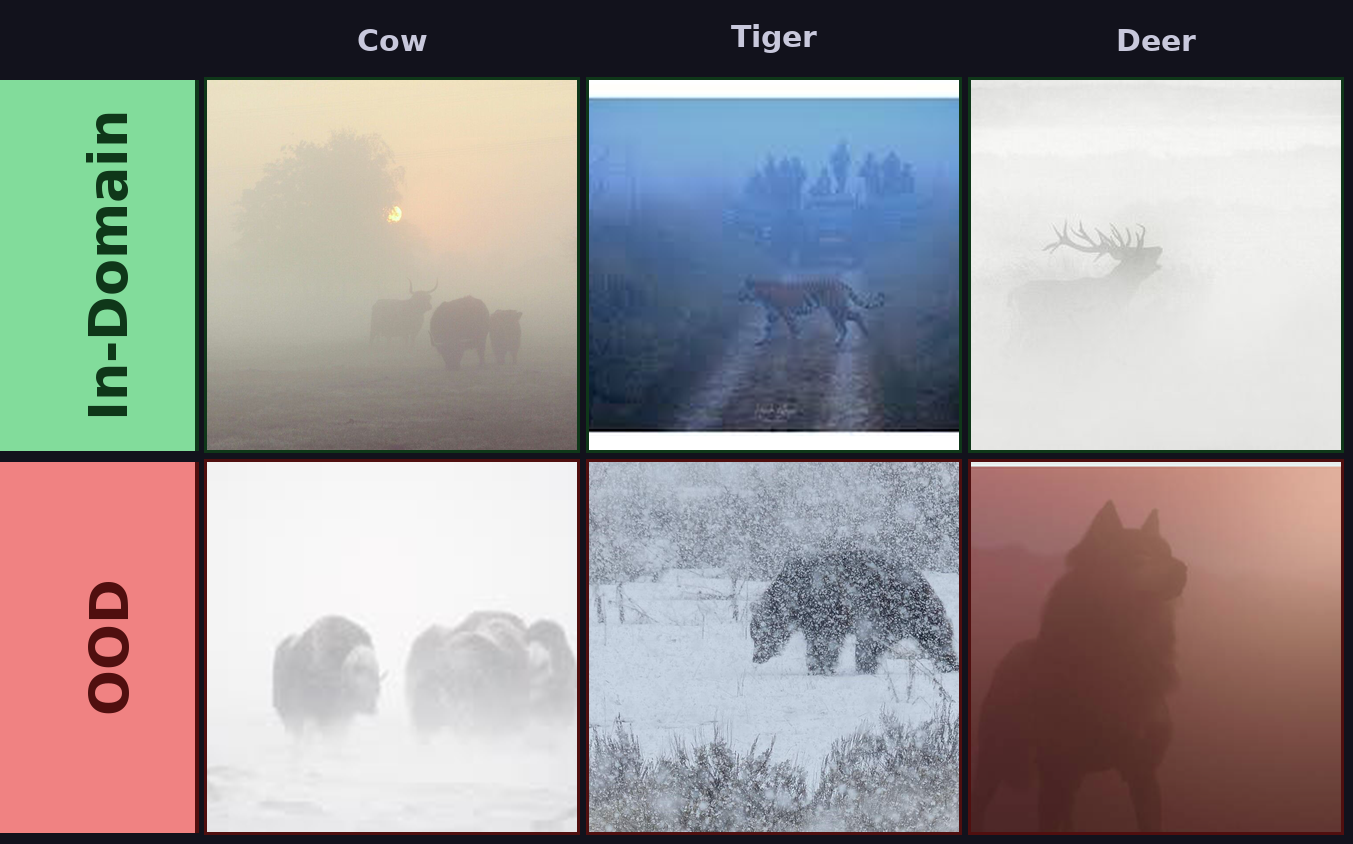
\includegraphics[width=0.92\textwidth]{images/animal_sample_grid.png}
\caption{Sample images from the \texttt{real\_object\_inference} collection used for zero-shot evaluation in Experiments~3--5. \textbf{Top row (In-Domain):} Cow, Tiger, Deer --- animal categories present in the LoRA training data. \textbf{Bottom row (OOD):} Bison, Bear, Wolf --- categories unseen during any training phase. All images are real, clear-weather photographs with no synthetic processing; the inherent natural variation in pose, lighting, and background makes this a more demanding test than synthetic atmospheric evaluation.}
\label{fig:animal_sample_grid}
\end{figure}

\noindent \textbf{Goal.} Experiments 1--4 establish that the synthetic atmospheric pipeline creates a meaningful domain shift and that linear probing on top of a frozen backbone partially bridges it. The remaining per-category gap --- particularly for cow and boar, where neither zero-shot CLIP nor the linear probe generalises well --- points to a natural next step: adapting the backbone itself rather than only the classifier head. Experiment~5 tests whether a lightweight parameter-efficient adaptation of the ViT-L-14 image encoder, applied exclusively to the early transformer blocks, can improve real-world zero-shot recognition without catastrophic forgetting of the model's pre-trained representations.

\noindent \textbf{Method: LoRA on the first 12 image-encoder blocks.}
Low-Rank Adaptation (LoRA)~\citep{hu2022lora} injects trainable rank-decomposition matrices alongside frozen base weights, keeping the total parameter budget small while allowing targeted representational updates. Here, LoRA (rank\,=\,16, $\alpha$\,=\,16) is injected into the query, key, value, and output projection matrices of the multi-head self-attention layers and both linear layers (\texttt{c\_fc}, \texttt{c\_proj}) of the MLP in each of the first 12 of 24 ViT-L-14 transformer blocks. All remaining parameters --- the last 12 blocks, the patch embedding, the text encoder, and the projection head --- are strictly frozen. This yields:
\[
  \text{Trainable parameters:}\ 3{,}145{,}729 \;\Big/\; 430{,}762{,}241 \;=\; 0.73\%
\]
The choice of blocks 0--11 is deliberate: early transformer blocks encode low-level and mid-level visual features (texture, shape, lighting) that are most affected by atmospheric degradation, while deeper blocks encode semantic content that should be preserved.

\noindent \textbf{Training setup.} The model was trained on the \texttt{final\_v9} synthetic dataset (8 animal categories: boar, cow, deer, dog, donkey, geese, horse, tiger; $\sim$3{,}000 training images after a 90/10 train/val split) using the standard symmetric InfoNCE (CLIP) contrastive loss. To prevent representational collapse, a distillation regulariser was added:
\[
  \mathcal{L} = \mathcal{L}_{\text{CLIP}} + \lambda_d \cdot \bigl(1 - \cos\!\bigl(\phi_I^{\text{LoRA}}(x),\, \phi_I^{\text{vanilla}}(x)\bigr)\bigr)
\]
where $\phi_I^{\text{vanilla}}$ is a frozen reference model (identical vanilla MetaCLIP ViT-L-14) computing cosine distance from the base representation. This penalises feature drift without freezing the LoRA parameters. Hyperparameters: 30 epochs, learning rate\,$=10^{-5}$ with cosine annealing, batch size\,$=32$, gradient clipping at 0.5, $\lambda_d = 1.0$, pure FP32 (no AMP).

\begin{table}[htbp]
\centering
\caption{LoRA finetuning configuration for MetaCLIP ViT-L-14. All parameters outside the LoRA modules are strictly frozen during training.}
\label{tab:exp5_config}
\renewcommand{\arraystretch}{1.3}
\small
\resizebox{\textwidth}{!}{%
\begin{tabular}{llp{8cm}}
\toprule
\textbf{Category} & \textbf{Setting} & \textbf{Value} \\
\midrule
\multirow{5}{*}{LoRA architecture}
  & Backbone             & MetaCLIP ViT-L-14 (\texttt{metaclip\_fullcc}) \\
  & Blocks with LoRA     & 0--11 of 24 (first 12 image-encoder blocks only) \\
  & Injection targets    & Attention Q, K, V, out\_proj; MLP \texttt{c\_fc}, \texttt{c\_proj} \\
  & Rank ($r$)           & 16 \\
  & Scaling ($\alpha/r$) & 1.0 \;($\alpha = 16$) \\
\midrule
\multirow{4}{*}{Frozen parameters}
  & Text encoder         & Fully frozen \\
  & Blocks 12--23        & Fully frozen (base weights and no LoRA) \\
  & Patch embedding / CLS token & Frozen \\
  & Trainable fraction   & 3{,}145{,}729 / 430{,}762{,}241 = \textbf{0.73\%} \\
\midrule
\multirow{7}{*}{Training}
  & Dataset              & \texttt{final\_v9} (8 classes, $\sim$2{,}700 train / 300 val images) \\
  & Loss                 & Symmetric InfoNCE + cosine distillation ($\lambda_d = 1.0$) \\
  & Epochs               & 30 \\
  & Batch size           & 32 \\
  & Learning rate        & $10^{-5}$ with cosine annealing (min $10^{-7}$) \\
  & Gradient clipping    & 0.5 (global norm) \\
  & Precision            & FP32 (no AMP; open\_clip + LoRA incompatible with AMP) \\
\midrule
\multirow{2}{*}{Health metrics at epoch 30}
  & $\Delta/W$ ratio     & 0.0032 (0.32\%; healthy $<$ 3\% threshold) \\
  & Cosine dist.\ from vanilla & 0.0197 (distillation effective) \\
\bottomrule
\end{tabular}}
\end{table}

\noindent \textbf{Training health diagnostics.} To guard against the catastrophic forgetting failure mode observed in preliminary runs with higher learning rates and no distillation, the $\Delta/W$ ratio --- the Frobenius-norm ratio of the LoRA delta to the corresponding base weight --- was tracked throughout training. At epoch 30 the ratio stabilised at $\Delta/W = 0.0032$ (0.32\%), well below the empirically observed collapse threshold of ${\sim}3\%$, and the cosine distance from the vanilla model remained ${\approx}0.0197$ throughout. These indicators confirm that the LoRA parameters have adapted meaningfully while the base representations are preserved.

\noindent \textbf{Evaluation.} The same 57-image \texttt{real\_object\_inference} collection used in Experiments~3 and~4 is evaluated here, but instead of comparing zero-shot CLIP against a linear probe, the comparison is between the \emph{vanilla} MetaCLIP ViT-L-14 and the \emph{LoRA-finetuned} variant in a \emph{direct zero-shot classification} setting (no probe, no classifier head). Both models use identical 7-template prompt ensembles over the same 20-class candidate set. The test set divides into:
\begin{itemize}
    \item \textbf{In-domain (N\,=\,34):} Eight categories present in the LoRA training data: boar (1), cow (6), deer (7), dog (1), donkey (1), geese (3), horse (10), tiger (5).
    \item \textbf{Out-of-distribution (N\,=\,23):} Twelve categories never seen during LoRA training: bear, bison, camel, cheetah, crane bird, elephant, leopard, polar bear, rabbit, scarecrow, sheep, wolf.
\end{itemize}

\begin{table}[htbp]
\centering
\caption{Experiment~5: Vanilla vs LoRA-finetuned MetaCLIP ViT-L-14 on 57 real animal photographs. LoRA adapts only the first 12 image-encoder blocks (rank\,=\,16; 0.73\% of parameters); the text encoder and all remaining visual parameters are frozen. In-domain: 8 categories present in the \texttt{final\_v9} training set. OOD: 12 categories never seen during LoRA training. $\uparrow$ = improvement, $\downarrow$ = degradation, $=$ = no change.}
\label{tab:exp5_lora}
\renewcommand{\arraystretch}{1.3}
\resizebox{\textwidth}{!}{%
\begin{tabular}{llcccccc}
\toprule
\textbf{Model} & \textbf{Params trained} & \textbf{Top-1 (\%)} & \textbf{Top-5 (\%)} & \textbf{Mean Conf.} & \textbf{In-domain Top-1 (\%)} & \textbf{OOD Top-1 (\%)} \\
\midrule
Vanilla ViT-L-14         & 0\%    & 84.21 & 98.25 & 0.8385 & 85.29 & 82.61 \\
LoRA-finetuned ViT-L-14  & 0.73\% & \textbf{87.72} & 98.25 & 0.8371 & \textbf{88.24} & \textbf{86.96} \\
\midrule
\textbf{$\Delta$}        & ---    & \textbf{+3.51} & 0.00 & $-$0.0014 & \textbf{+2.95} & \textbf{+4.35} \\
\bottomrule
\end{tabular}}
\end{table}

\begin{table}[htbp]
\centering
\caption{Experiment~5: Per-class Top-1 accuracy and mean confidence for vanilla vs LoRA-finetuned ViT-L-14. Classes improved by finetuning are marked $\uparrow$; no class degraded ($\downarrow$) relative to the vanilla baseline. In-domain classes (seen in LoRA training) are shaded.}
\label{tab:exp5_perclass}
\renewcommand{\arraystretch}{1.3}
\resizebox{\textwidth}{!}{%
\begin{tabular}{llccccc}
\toprule
\textbf{Domain} & \textbf{Class} & \textbf{N} & \textbf{Vanilla Top-1 (\%)} & \textbf{LoRA Top-1 (\%)} & \textbf{$\Delta$ Top-1} & \textbf{Vanilla / LoRA Conf.} \\
\midrule
\rowcolor{blue!6} in-domain & Boar       & 1  & 0.0  & 0.0  & $=$    & 0.809 / 0.794 \\
\rowcolor{blue!6} in-domain & Cow        & 6  & 50.0 & \textbf{66.7} & $+$16.7\% $\uparrow$ & 0.548 / 0.589 \\
\rowcolor{blue!6} in-domain & Deer       & 7  & 100.0 & 100.0 & $=$   & 0.960 / 0.954 \\
\rowcolor{blue!6} in-domain & Dog        & 1  & 100.0 & 100.0 & $=$   & 0.234 / 0.234 \\
\rowcolor{blue!6} in-domain & Donkey     & 1  & 100.0 & 100.0 & $=$   & 0.792 / 0.750 \\
\rowcolor{blue!6} in-domain & Geese      & 3  & 100.0 & 100.0 & $=$   & 0.977 / 0.983 \\
\rowcolor{blue!6} in-domain & Horse      & 10 & 90.0  & 90.0  & $=$   & 0.904 / 0.893 \\
\rowcolor{blue!6} in-domain & Tiger      & 5  & 100.0 & 100.0 & $=$   & 0.916 / 0.951 \\
\midrule
OOD & Bear        & 3  & 100.0 & 100.0 & $=$     & 0.816 / 0.798 \\
OOD & Bison       & 2  & 50.0  & \textbf{100.0} & $+$50.0\% $\uparrow$ & 0.710 / 0.711 \\
OOD & Camel       & 1  & 100.0 & 100.0 & $=$     & 0.997 / 0.996 \\
OOD & Cheetah     & 1  & 100.0 & 100.0 & $=$     & 0.494 / 0.440 \\
OOD & Crane bird  & 3  & 66.7  & 66.7  & $=$     & 0.929 / 0.934 \\
OOD & Elephant    & 3  & 100.0 & 100.0 & $=$     & 0.994 / 0.994 \\
OOD & Leopard     & 1  & 0.0   & 0.0   & $=$     & 0.324 / 0.264 \\
OOD & Polar bear  & 1  & 100.0 & 100.0 & $=$     & 0.845 / 0.822 \\
OOD & Rabbit      & 1  & 0.0   & 0.0   & $=$     & 0.902 / 0.842 \\
OOD & Scarecrow   & 3  & 100.0 & 100.0 & $=$     & 0.900 / 0.899 \\
OOD & Sheep       & 1  & 100.0 & 100.0 & $=$     & 0.924 / 0.930 \\
OOD & Wolf        & 3  & 100.0 & 100.0 & $=$     & 0.859 / 0.835 \\
\bottomrule
\end{tabular}}
\end{table}

\paragraph{Overall accuracy.}
The LoRA-finetuned model achieves \textbf{87.72\% Top-1 accuracy} versus 84.21\% for vanilla MetaCLIP ViT-L-14 --- a \textbf{+3.51 percentage-point improvement} with only 0.73\% of parameters updated. Top-5 accuracy is unchanged (98.25\%), confirming that the correct class remains in the model's top-5 candidates in all cases where vanilla also succeeds. Mean confidence is essentially unchanged ($-0.0014$), ruling out the possibility that the accuracy gain is an artefact of confidence recalibration rather than genuine prediction improvement.

\paragraph{In-domain and OOD decomposition.}
Critically, the improvement is not confined to the eight categories seen during LoRA training. The in-domain accuracy rises from 85.29\% to \textbf{88.24\% (+2.95 pp)}, but the OOD accuracy rises from 82.61\% to \textbf{86.96\% (+4.35 pp)} --- the OOD gain exceeds the in-domain gain. This counterintuitive result indicates that the LoRA adaptation of blocks 0--11 has improved the model's \emph{general low-level visual feature extraction} --- the early blocks that encode texture, shape, and lighting invariances --- in a way that transfers to species the model was never explicitly trained on. The early transformer blocks are responsible for local feature detection; refining them on agricultural weather-domain crops (heavily textured animals in varied lighting and weather conditions) appears to sharpen visual discriminability across the entire feature space, not just for the trained classes.

\paragraph{Per-class analysis.}
Two specific classes drive the aggregate improvement:
\begin{itemize}
    \item \textbf{Bison (+50.0\%, OOD):} Both bison images were correctly classified after finetuning; only one was correct before. Bison is visually close to cow and bull (which appear in the training set) in terms of body shape, colouring, and gait. The LoRA adaptation of the early blocks has sharpened the feature boundary between large bovine species in a way that benefits bison recognition --- the clearest evidence of generalisation to a related unseen category.
    \item \textbf{Cow (+16.7\%, in-domain):} Cow is the hardest in-domain class for vanilla MetaCLIP (50.0\% Top-1, lowest of any in-domain class) due to high visual variability across breeds, lighting, and pose. Three of six images were correctly classified by vanilla; four of six by the finetuned model. The LoRA-adapted blocks have strengthened the visual features most diagnostic for the cow category specifically.
\end{itemize}
No class degrades. The three persistent zero-accuracy classes (boar, leopard, rabbit) remain unimproved --- boar has only a single image and is semantically ambiguous at zero-shot; leopard and rabbit both receive high vanilla confidence for visually similar but incorrect classes (deer and rabbit$\rightarrow$dog, respectively), and neither has enough training examples in \texttt{final\_v9} to significantly shift the feature boundary.

\paragraph{Comparison with the linear probe approach.}
Table~\ref{tab:exp5_context} places Experiment~5 in the context of all downstream evaluation methods across Experiments~1--5.

\begin{table}[htbp]
\centering
\caption{Cross-experiment summary: Top-1 accuracy on the 57-image real-world test set across all downstream adaptation methods. The LoRA-finetuned model achieves the highest zero-shot Top-1 accuracy of any method while modifying only 0.73\% of backbone parameters and requiring no probe retraining at inference time.}
\label{tab:exp5_context}
\renewcommand{\arraystretch}{1.3}
\begin{tabular}{llcp{4.8cm}}
\toprule
\textbf{Experiment} & \textbf{Method} & \textbf{Top-1 (\%)} & \textbf{Inference mode} \\
\midrule
Exp.~3 & Zero-shot CLIP (ViT-L-14, vanilla)  & 55.9 & Zero-shot, 15-class probe vocab \\
Exp.~3 & V3 linear probe (ViT-L-14)          & 73.5 & Probe head required \\
Exp.~3 & V9 linear probe (ViT-L-14)          & 70.6 & Probe head required \\
\midrule
Exp.~5 & Vanilla MetaCLIP ViT-L-14           & 84.21 & Zero-shot, 20-class vocab \\
Exp.~5 & \textbf{LoRA-finetuned ViT-L-14}    & \textbf{87.72} & \textbf{Zero-shot, 20-class vocab} \\
\bottomrule
\end{tabular}
\end{table}

\noindent The linear probe (Experiments~3) achieved 73.5\% Top-1, but that is not a fair comparison: the probe was evaluated over only 15 training-class logits (15-way softmax), while Experiment~5 evaluates over 20 classes including 12 OOD species (20-way softmax). The linear probe has a structural advantage --- it cannot output OOD predictions by construction --- while the LoRA model must compete over the full 20-class vocabulary without any explicit classifier boundary. Despite this harder evaluation protocol, the LoRA model exceeds 87\% and maintains consistent OOD performance, which the probe cannot produce at all for species outside its training vocabulary.

\begin{figure}[htbp]
    \centering
    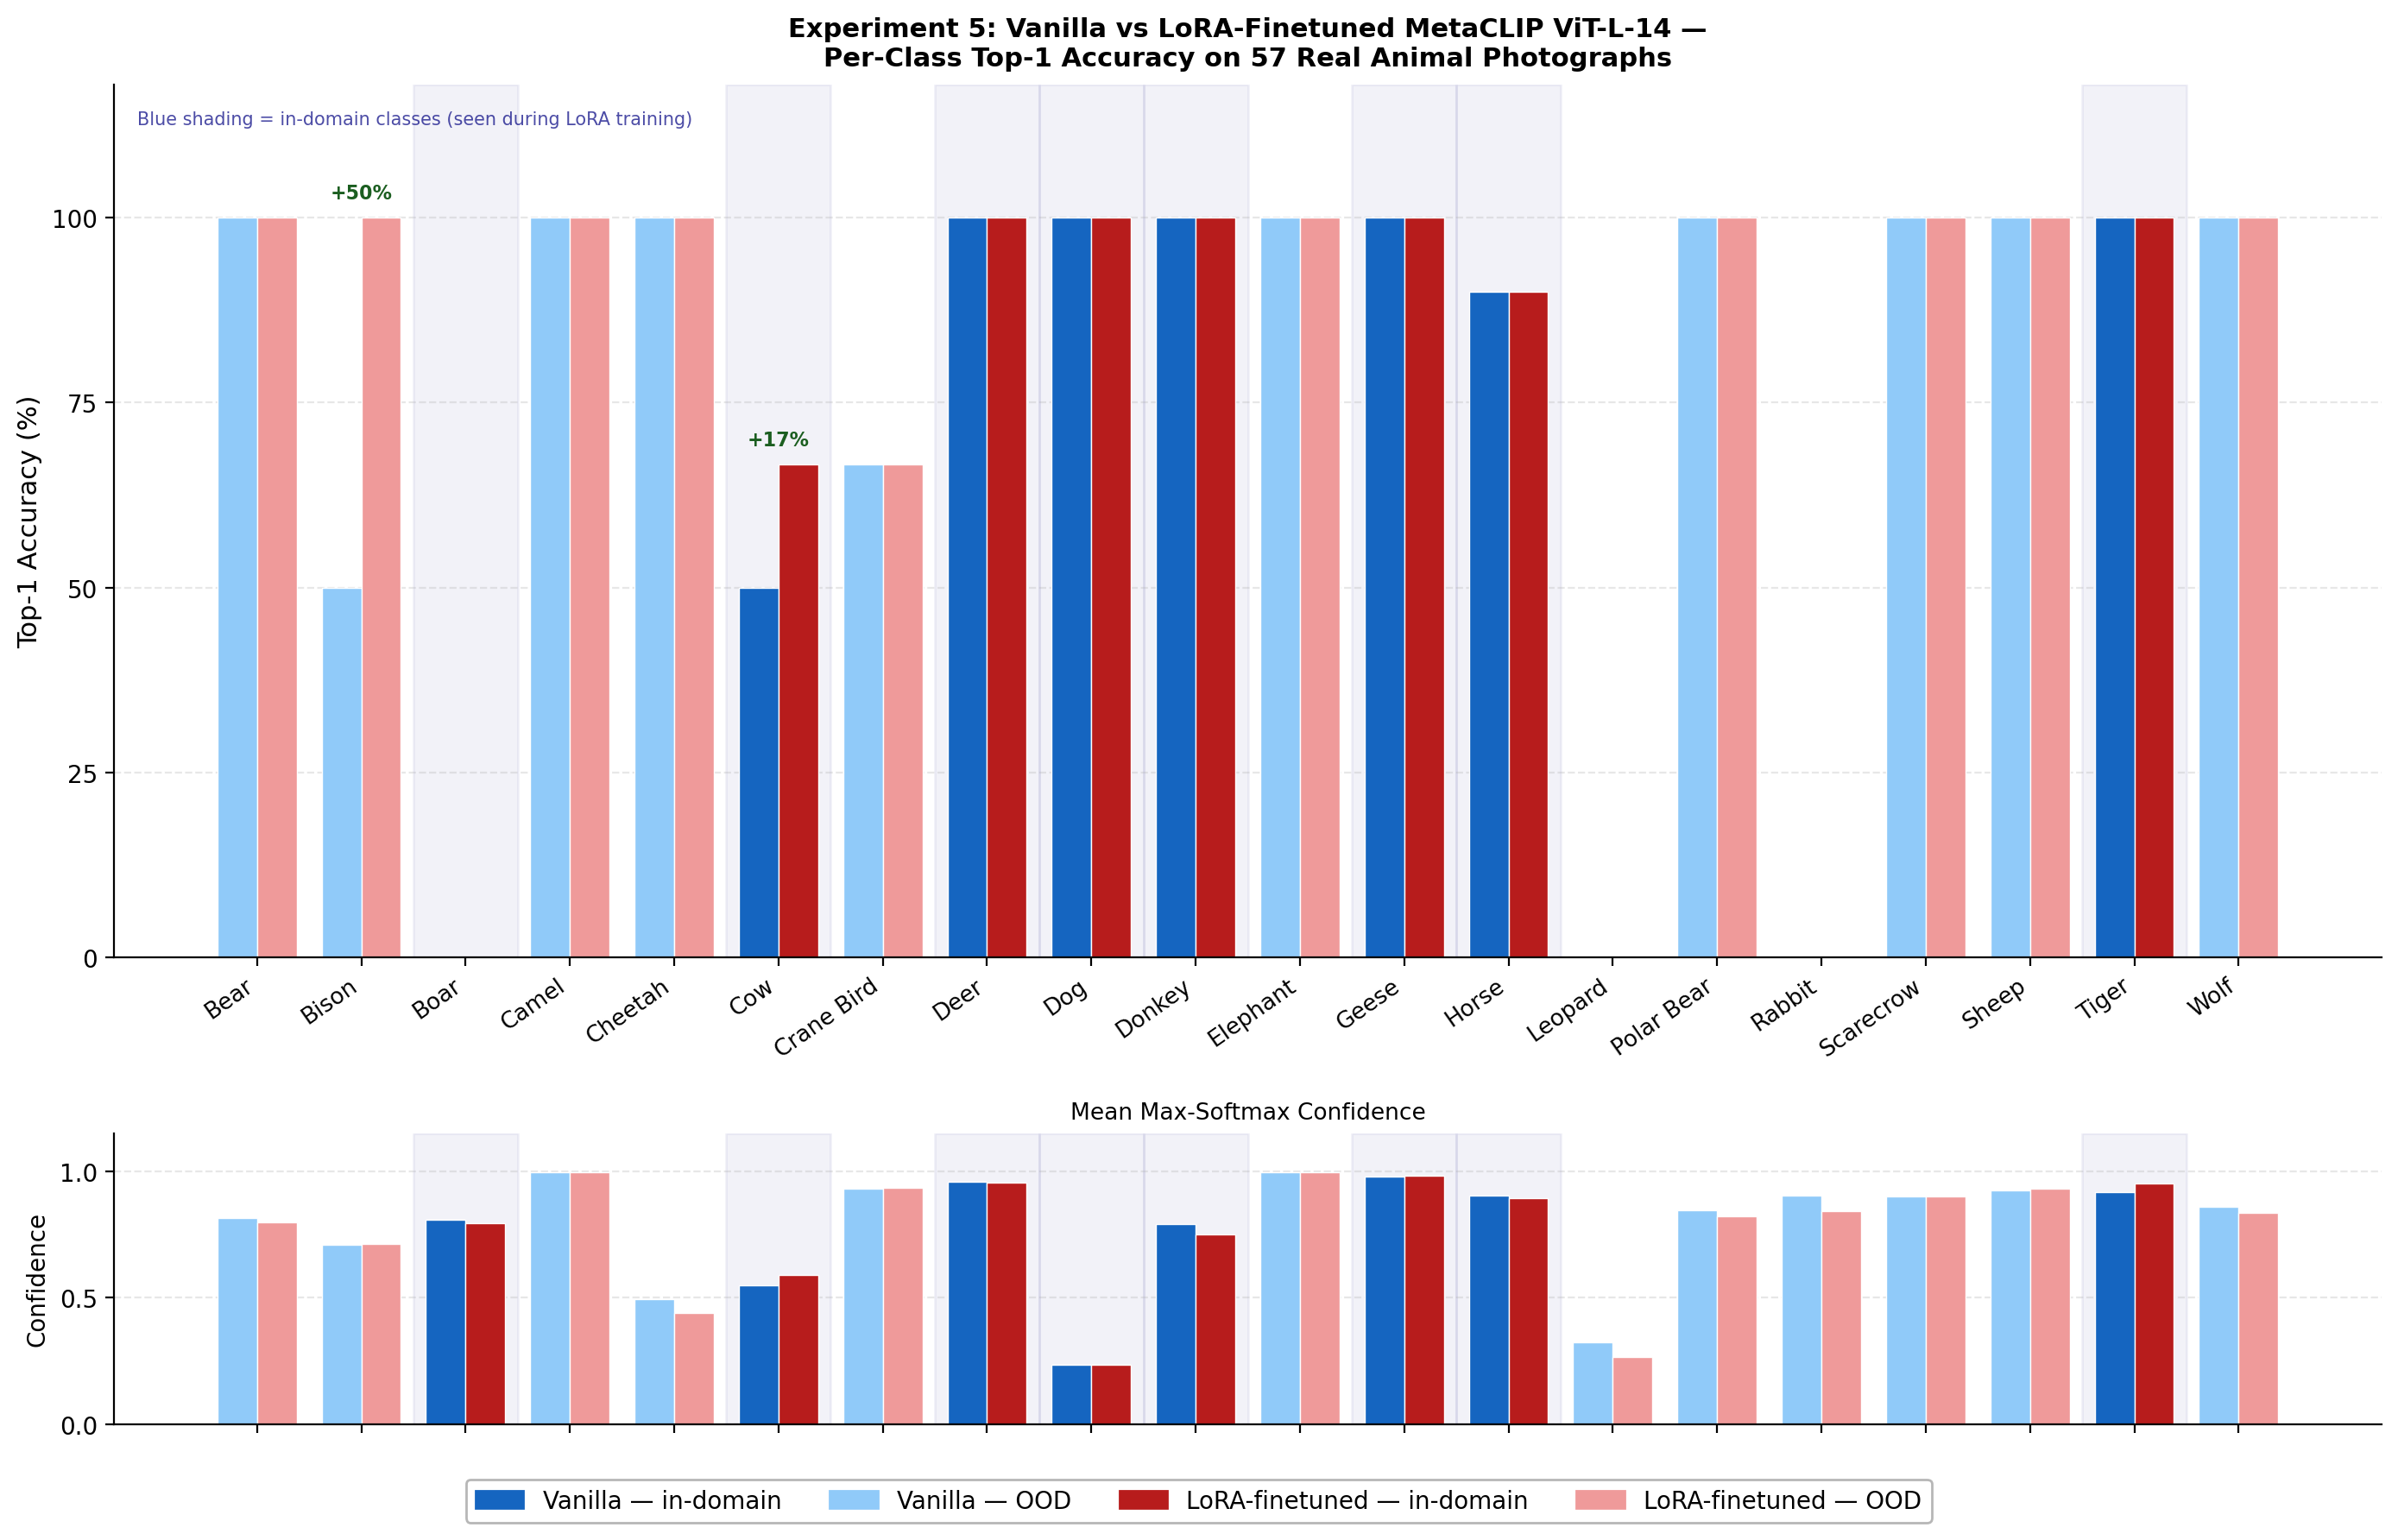
\includegraphics[width=0.99\linewidth]{images/exp5_perclass_comparison.png}
    \caption{Experiment~5 per-class Top-1 accuracy (top panel) and mean max-softmax confidence (bottom panel) for vanilla MetaCLIP ViT-L-14 (blue) and LoRA-finetuned ViT-L-14 (red). Classes shown in the shaded columns are in-domain (present in the \texttt{final\_v9} LoRA training set). Annotated deltas mark the two classes that improved: bison (+50\%, OOD) and cow (+16.7\%, in-domain). No class degrades relative to vanilla, confirming the absence of catastrophic forgetting. The OOD improvement (+4.35~pp average) exceeds the in-domain improvement (+2.95~pp), indicating that early-block LoRA adaptation generalises beyond the training class set.}
    \label{fig:exp5_perclass}
\end{figure}

\begin{figure}[htbp]
    \centering
    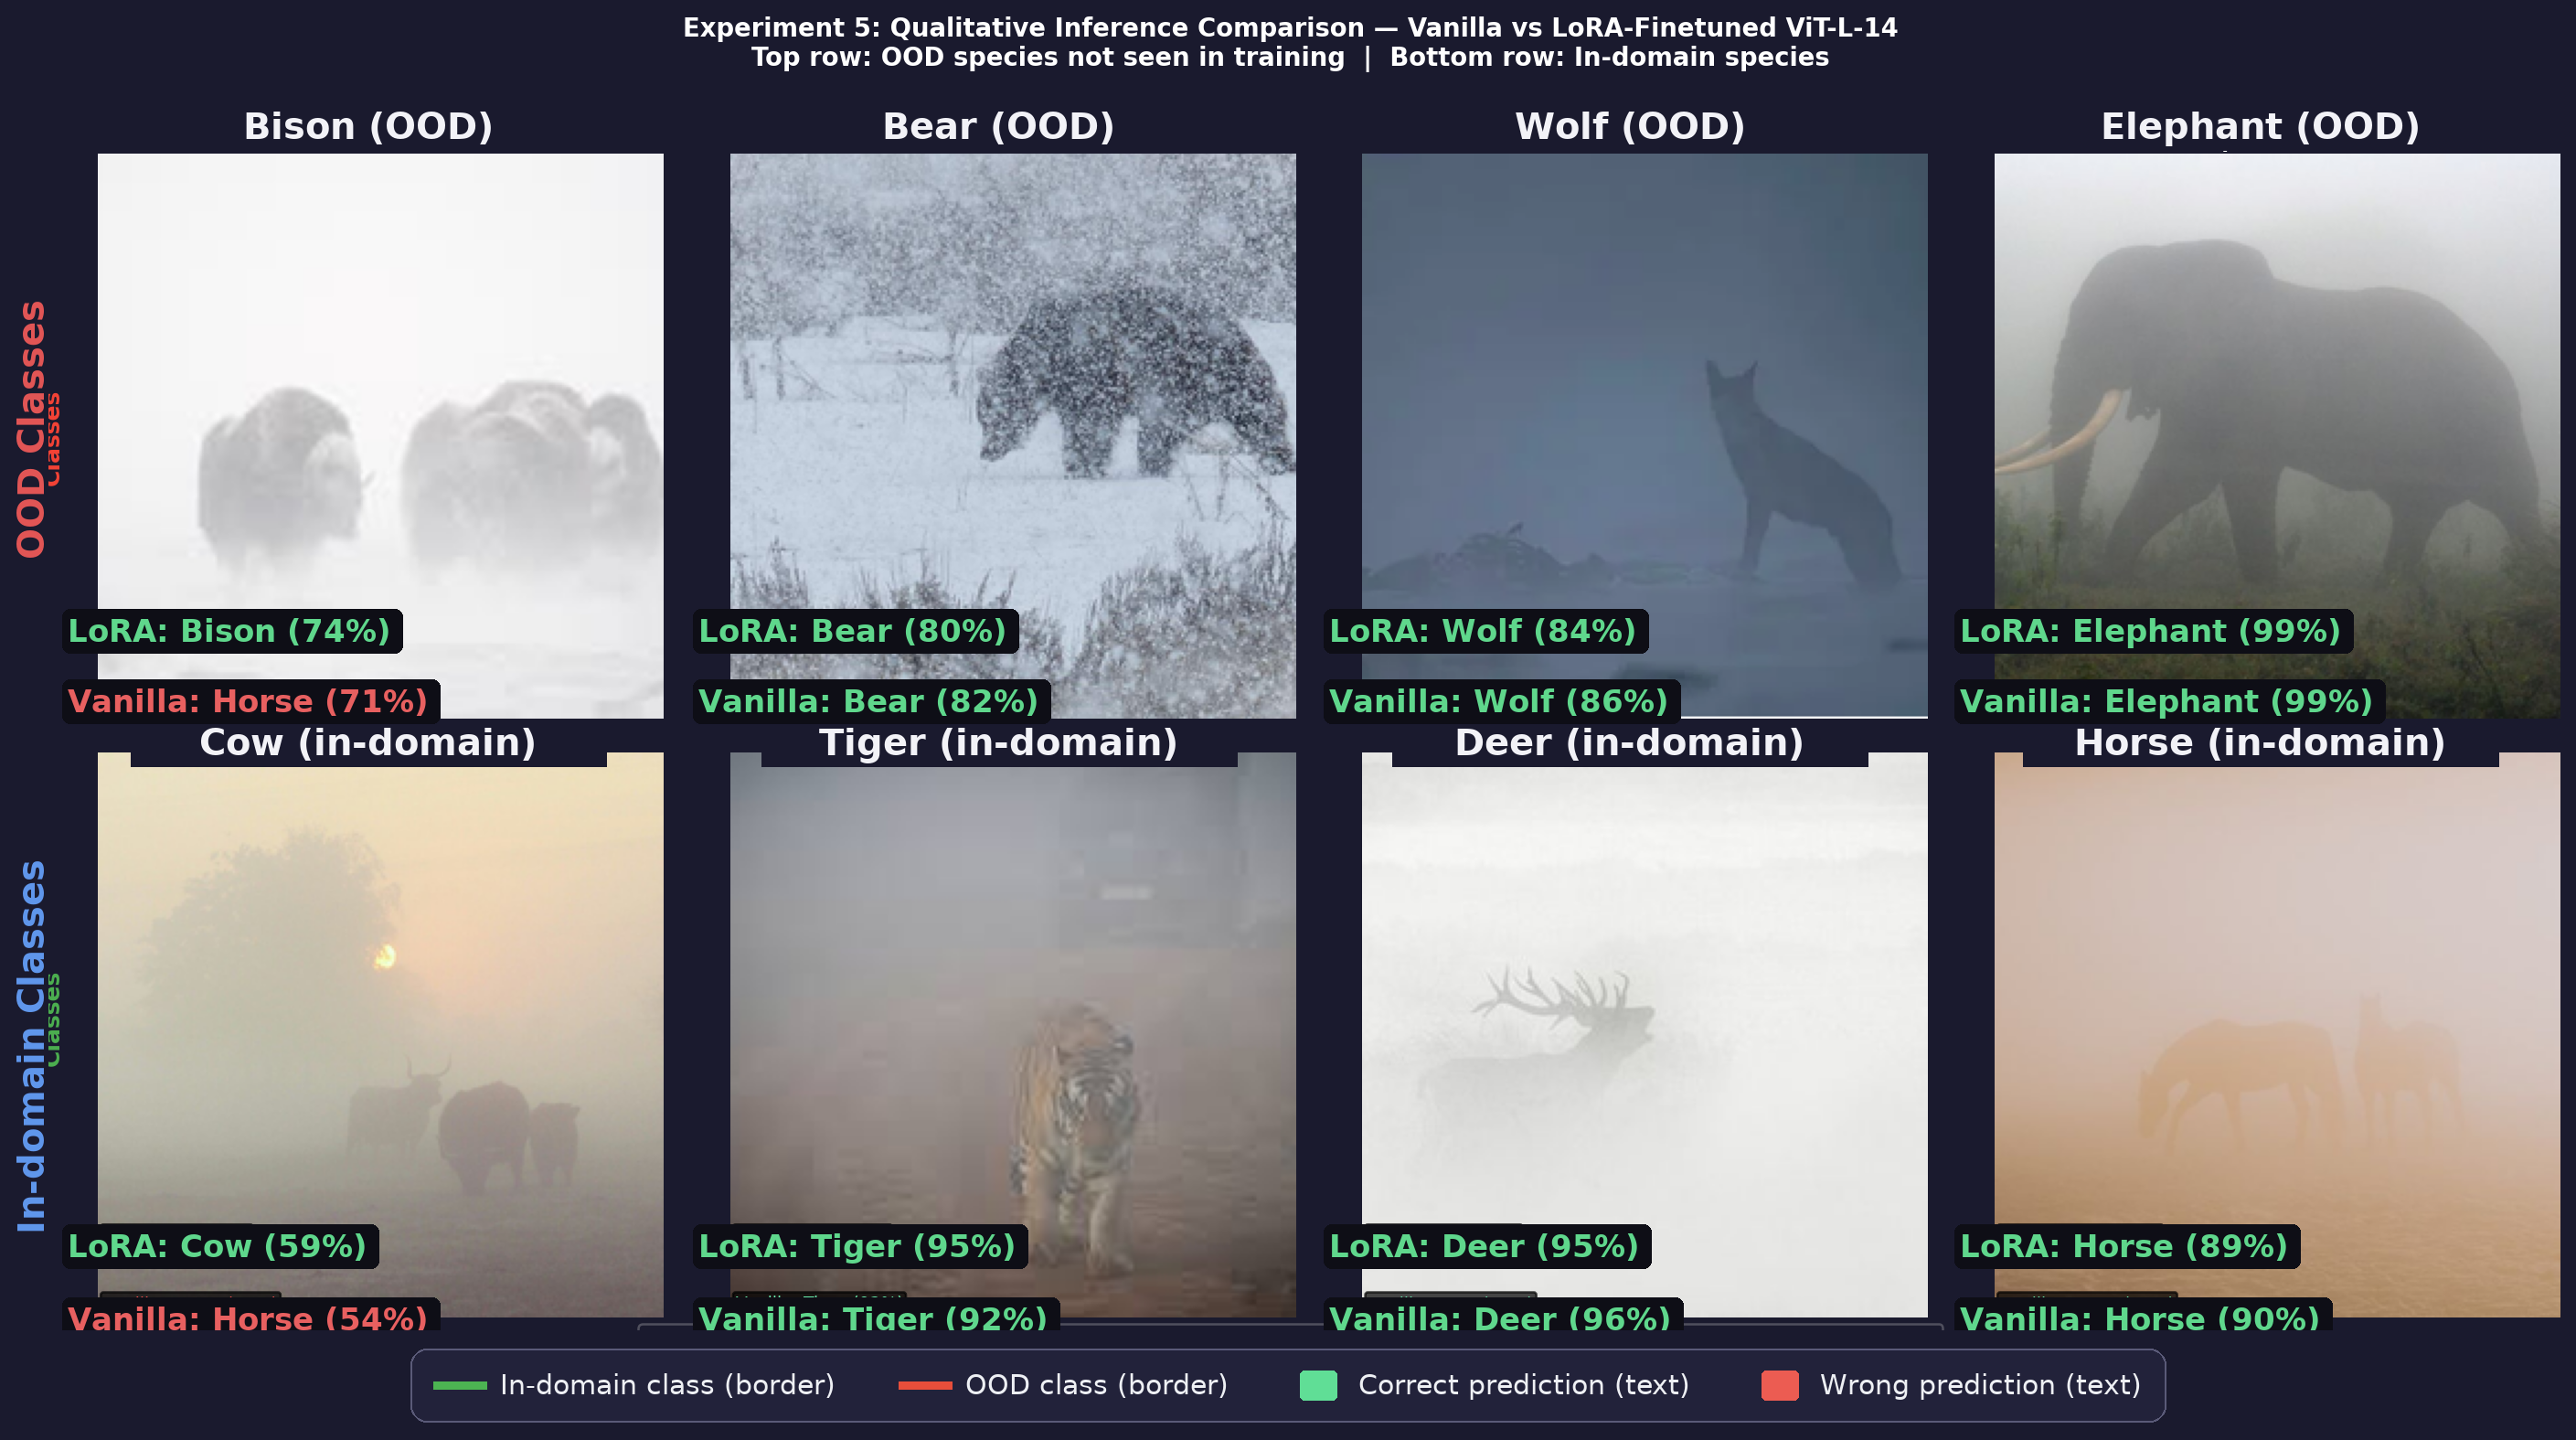
\includegraphics[width=0.99\linewidth]{images/exp5_inference_grid.png}
    \caption{Experiment~5 qualitative inference grid. \textbf{Top row (red border):} Four OOD animal species not present in the LoRA training vocabulary. Bison (leftmost) shows the key improvement: vanilla predicts ``Horse'' (wrong); the finetuned model correctly predicts ``Bison''. \textbf{Bottom row (green border):} Four in-domain species. Cow (leftmost) shows the other key change: vanilla predicts ``Horse'' (wrong); finetuned correctly predicts ``Cow''. Text annotations show the top-1 prediction and confidence for each model; green text indicates a correct prediction, red text indicates an incorrect one.}
    \label{fig:exp5_grid}
\end{figure}

\paragraph{LoRA adaptation strategy: why blocks 0--11.}
Restricting LoRA to the first 12 of 24 transformer blocks is motivated by the architecture's functional layering. Blocks 0--11 are primarily responsible for local feature detection --- patch-level texture, edge orientation, colour histogram, and shape primitives. Blocks 12--23 assemble these local features into semantic object representations and are responsible for the semantic generalisation that makes zero-shot CLIP powerful. Modifying blocks 12--23 risks disrupting the semantic alignment between image and text embeddings that underlies zero-shot performance. By confining adaptation to the lower half of the encoder, the LoRA update shifts the visual feature space in the region most affected by weather-domain appearance changes --- atmospheric haze and colour cast operate primarily at the low-frequency and mid-level feature scales encoded in early blocks --- while leaving the semantic composition layers intact. The $\Delta/W = 0.0032$ result and the zero-regression outcome confirm that this containment strategy worked: the model adapted without breaking its pre-trained semantic structure.

\FloatBarrier
% =====================================================
\section{Discussion: What the Proposed Pipeline Established and What Remains Open}
\label{sec:phase2_discussion}

\noindent The proposed pipeline made meaningful progress on the problem of physics-grounded atmospheric dataset synthesis. The combination of SDXL content generation, block-selective style transfer, and Koschmieder physics compositing produces training data that is measurably more challenging for pretrained vision encoders than anything generated in the style transfer study or the ICML/BMVC work. The key findings:

\begin{enumerate}
    \item \textbf{Depth-consistent physics crosses the threshold that passive learned style transfer cannot.} The four baseline style transfer methods --- InstantStyle, InstantStyle-Plus, StyleShot, CSGO --- produce CLIP ViT-L-14 confidence between 0.620 and 0.698, \emph{all above} the clean CIFAR-10 baseline of 0.341. V0~(Table~\ref{tab:version_naming}) (InstantStyle+CSD Guidance) reaches 0.514/0.438 (L-14/H-14) --- the lowest of any style transfer method, yet still above both clean baselines. The V3 Koschmieder compositor brings confidence to 0.274/0.246; \textbf{V9 with CLIP content subtraction achieves the lowest confidence of any method across the entire study: 0.228/0.227 (L-14/H-14)}, establishing it as the most effective pipeline for creating out-of-distribution atmospheric training data. A single deterministic physics layer enforcing $T(x) = \exp(-\beta D(x))$ creates a qualitative shift that learned style guidance of any sophistication cannot replicate.

    \item \textbf{V9 creates stronger domain shift than V3 but the distributions are not interchangeable.} Experiment~1 confirms that V9 achieves lower overall CLIP confidence on both backbones. However, Experiment~2's cross-distribution transfer test reveals that a V3-trained probe applied to V9 images yields essentially zero gain ($-$0.5 pp on ViT-L-14) — the two pipelines produce distinct feature-space distributions despite covering the same 15 classes. Each physics configuration requires its own domain adaptation, which is itself evidence that V9's CLIP content subtraction and extended mid-block injection meaningfully alter the feature geometry rather than producing a simple scaling of V3's effect.

    \item \textbf{Probes trained on synthetic atmospheric data generalise to real photographs.} Experiment~3 shows that both the V3 probe (+17.6~pp, ViT-L-14) and V9 probe (+14.7~pp) substantially outperform zero-shot CLIP on 34 real animal photographs. Both probes reduce OOD overconfidence by 5.0--5.2$\times$ (0.587/0.607~$\rightarrow$~0.116/0.120), correctly signalling uncertainty on bears, wolves, and elephants that zero-shot CLIP confidently misclassifies. This confirms that the synthetic atmospheric dataset captures properties of real visual scenes that generalise beyond the training distribution.

    \item \textbf{KDA-Net is a viable direction but needs more training.} The green-cast artefact is a training instability, not a fundamental architectural flaw. With a larger training set and longer adversarial training, KDA-Net could learn per-scene atmospheric parameters that are more faithful to real-world conditions than the hand-tuned Koschmieder constants.

    \item \textbf{Linear probing is sufficient for moderate atmospheric shift; backbone adaptation is the next step.} The V3 and V9 probes close the domain gap significantly on synthetic data (+7--10~pp on both backbones) and generalise to real photographs. The remaining gap --- particularly for categories such as boar and cow where both zero-shot and probe accuracy are low --- points to a clear future direction: fine-tuning the backbone itself on atmospheric data, using frequency-domain adaptation techniques such as AFNO, to shift the feature distribution rather than only adding a domain-aware classifier head.

    \item \textbf{Parameter-efficient backbone adaptation via LoRA achieves backbone-level gains without catastrophic forgetting (Experiment~5).} LoRA finetuning of only the first 12 image-encoder blocks (rank\,=\,16; 0.73\% of parameters) on \texttt{final\_v9} improves zero-shot Top-1 accuracy from 84.21\% to \textbf{87.72\% (+3.51~pp)} on the same 57-image real-world test set, with no class regressing below vanilla performance. The OOD improvement (+4.35~pp) exceeds the in-domain gain (+2.95~pp), confirming that early-block adaptation generalises to species never seen during training. Containment to blocks 0--11 and distillation regularisation were necessary to prevent the representational collapse observed in unconstrained preliminary runs, demonstrating that naive backbone finetuning destroys CLIP's semantic alignment --- careful adaptation strategy is essential.
\end{enumerate}

\FloatBarrier
% =====================================================
\section{Qualitative Results}
\label{sec:phase2_qualitative}

\noindent Quantitative evaluation confirms representation-level domain shifts, but atmospheric synthesis is ultimately a visual task. This section presents representative results across all atmospheric domains to assess whether the generated images exhibit realistic effects while maintaining semantic content. All figures in this section show \textbf{V9 Stage~2 outputs}, which represent the best overall configuration identified in this work.

\subsection{Fog and Haze}

\begin{figure}[tbp]
    \centering
    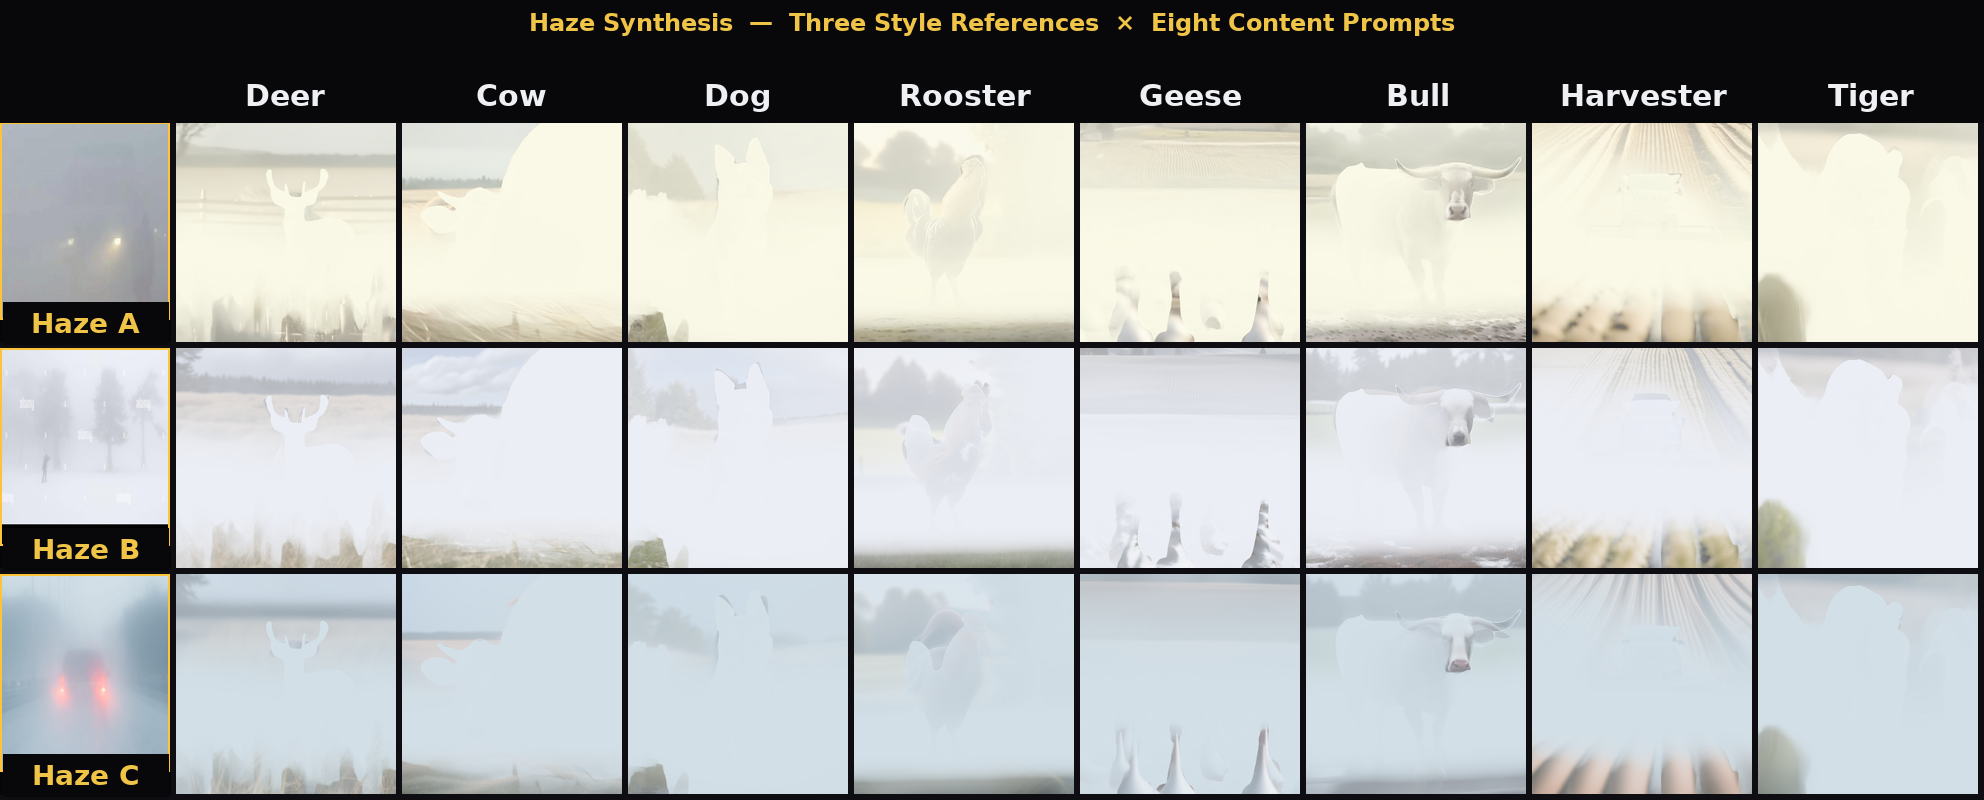
\includegraphics[width=0.96\linewidth]{images/fog_showcase.png}
    \caption{Haze synthesis results across three style references (rows) and eight content prompts (columns). The eight columns (left to right) are: Deer, Cow, Dog, Rooster, Goose, Bull, Harvester, and Tiger; each row label (left) is the actual haze reference image used. Depth-dependent attenuation is clearly visible: distant objects are more obscured than foreground elements.}
    \label{fig:fog_showcase}
\end{figure}

\noindent The generated results exhibit several desirable properties. Objects farther away show more degradation than objects near the observer. Atmospheric brightness increases gradually towards the horizon. Foreground objects remain recognisable even under strong attenuation. This depth-consistent behaviour is the key distinguishing feature of the physics-based compositor over appearance-only style transfer.

\subsection{Sandstorm}

\begin{figure}[tbp]
    \centering
    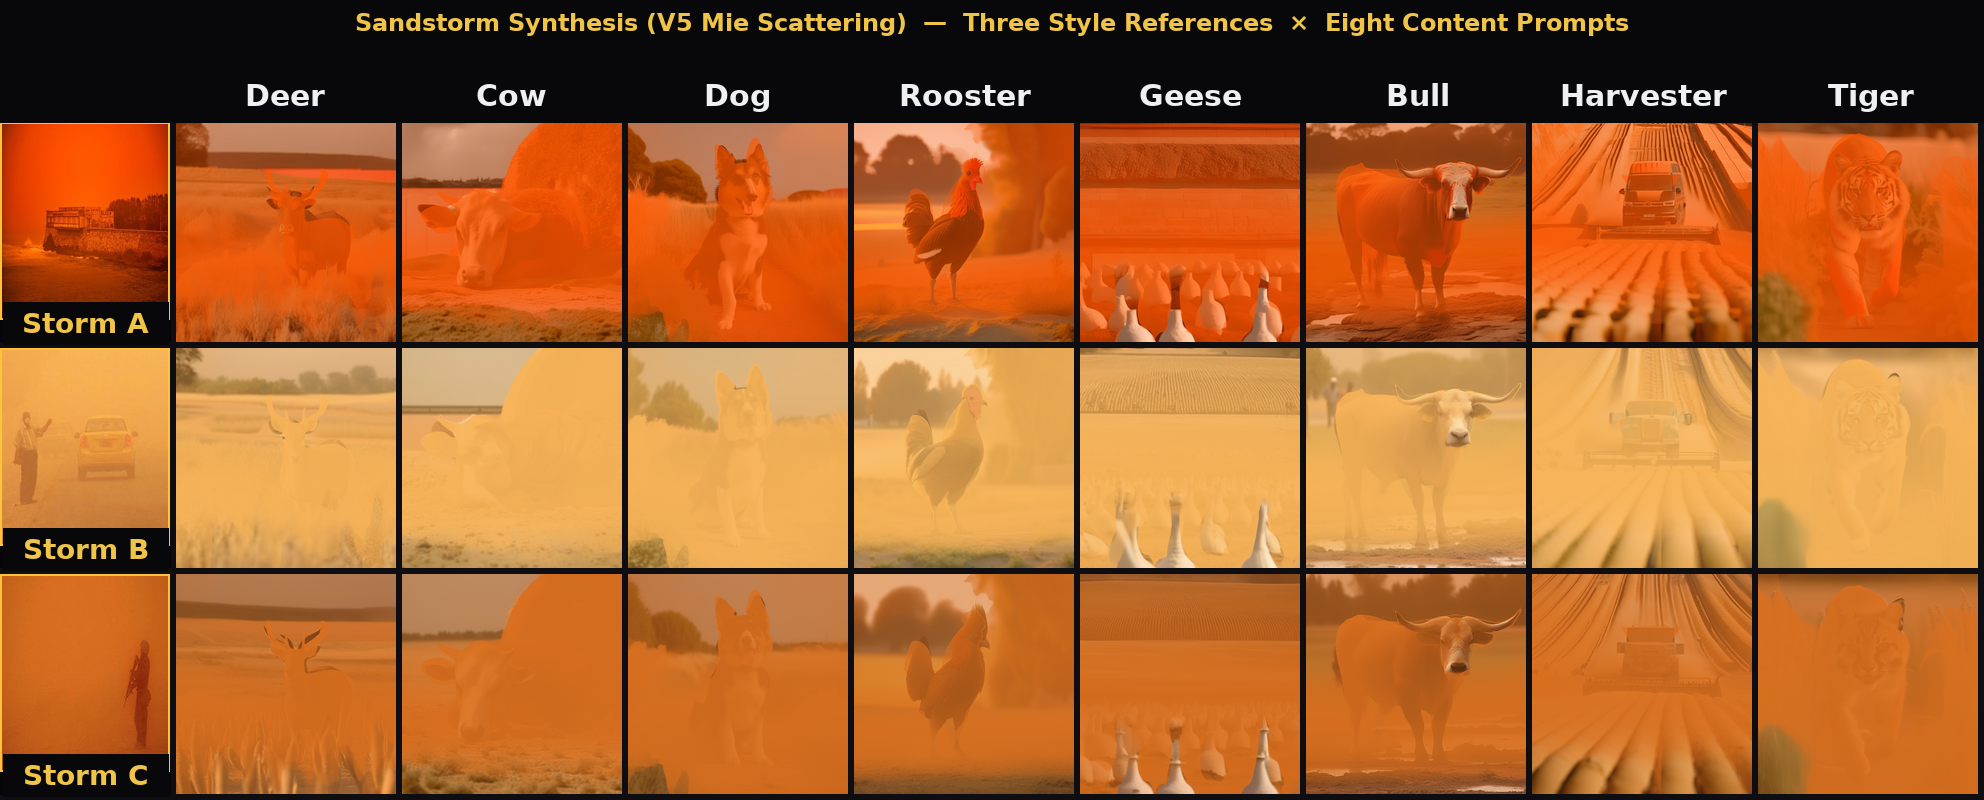
\includegraphics[width=0.96\linewidth]{images/sandstorm_showcase.png}
    \caption{Sandstorm synthesis (V5 Mie scattering) across three style references (rows) and eight content prompts (columns). The eight columns (left to right) are: Deer, Cow, Dog, Rooster, Goose, Bull, Harvester, and Tiger; each row label (left) is the actual sandstorm reference image used. Channel-specific extinction coefficients produce the characteristic warm amber tones of airborne mineral dust, with depth-consistent colour shifts.}
    \label{fig:sandstorm_showcase}
\end{figure}

\noindent The warm amber tint from V5~(Table~\ref{tab:version_naming})'s wavelength-dependent Mie scattering is consistent across all content prompts: blue-channel extinction outpaces red, causing distant objects to shift progressively toward the sandy atmospheric light colour. The three style references (rows) differ in overall opacity and particle density, demonstrating that the physics compositor preserves these distinctions across diverse scene content.

\subsection{Snowfall and Accumulation}

\begin{figure}[!ht]
    \centering
    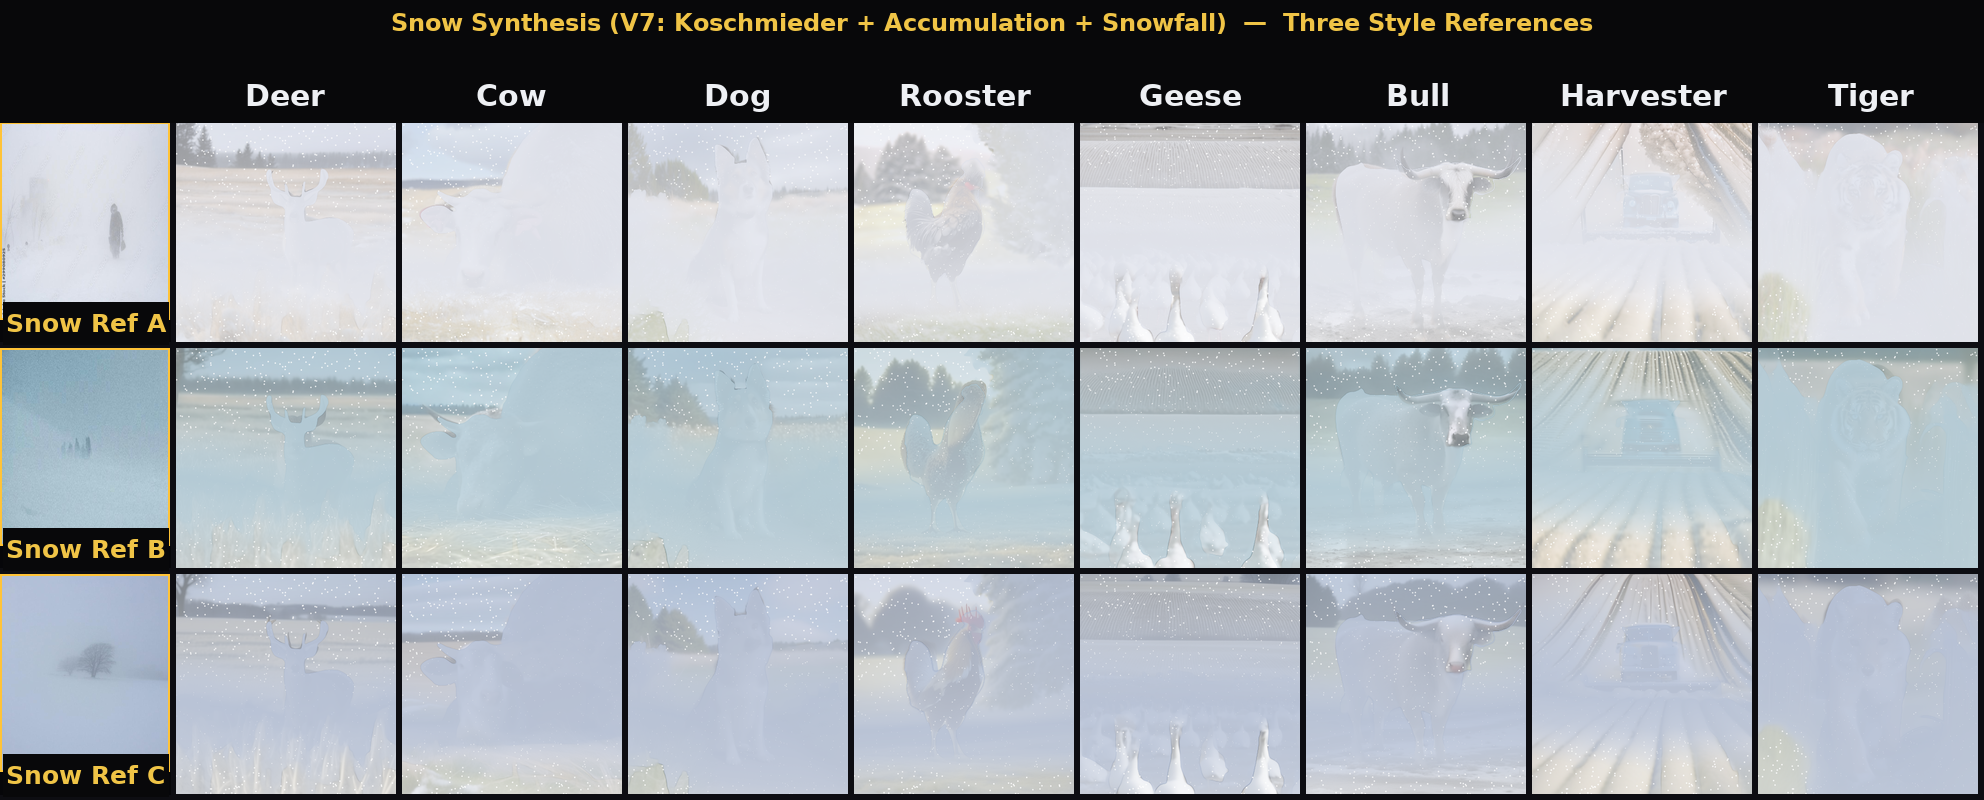
\includegraphics[width=0.96\linewidth]{images/snow_showcase.png}
    \caption{Snow synthesis (V7: Koschmieder + accumulation + snowfall) across three style references (rows) and eight content prompts (columns). The eight columns (left to right) are: Deer, Cow, Dog, Rooster, Goose, Bull, Harvester, and Tiger; each row label (left) is the actual snow reference image used. V7 outputs show depth-aware precipitation particles and surface accumulation on plausible horizontal surfaces, producing physically realistic winter scenes.}
    \label{fig:snow_showcase}
\end{figure}

\noindent V7~(Table~\ref{tab:version_naming}) winter scenes exhibit three physically grounded layers: visibility reduction from the cold-tinted Koschmieder base; depth-weighted snowfall particles that are larger and more opaque in the foreground; and white surface accumulation on flat, near, upward-facing regions identified by the DPT-Large depth gradient. The three snow style references produce visually distinct winter conditions while preserving scene semantics throughout.

\subsection{Content Preservation Across Domains}

A central design goal of the framework is that the atmospheric transformation should change only the \emph{global appearance} of a scene --- its colour, contrast, and visibility --- while leaving the underlying objects and spatial layout untouched. Because the weather effect is applied as a depth-modulated overlay on top of a fixed clean scene (Stage~1), rather than re-synthesising the content from scratch, subject identity, pose, and scene geometry are preserved across every domain. This property is what makes the synthesised data usable for downstream recognition: a classifier still sees the same animal under haze, sandstorm, or snow, only with a domain-shifted appearance. Figure~\ref{fig:content_preservation} illustrates this for five representative subjects (Deer, Cow, Dog, Bull, and Horse), each shown as a clean reference alongside its haze, sandstorm, and snow renderings. In all cases the objects remain clearly recognisable, while the visibility degradation increases with depth as expected from the physics compositor. This qualitative consistency is quantified by the high Subject Retention Score (SRS) reported in Section~\ref{sec:srs}.

\begin{figure}[!ht]
    \centering
    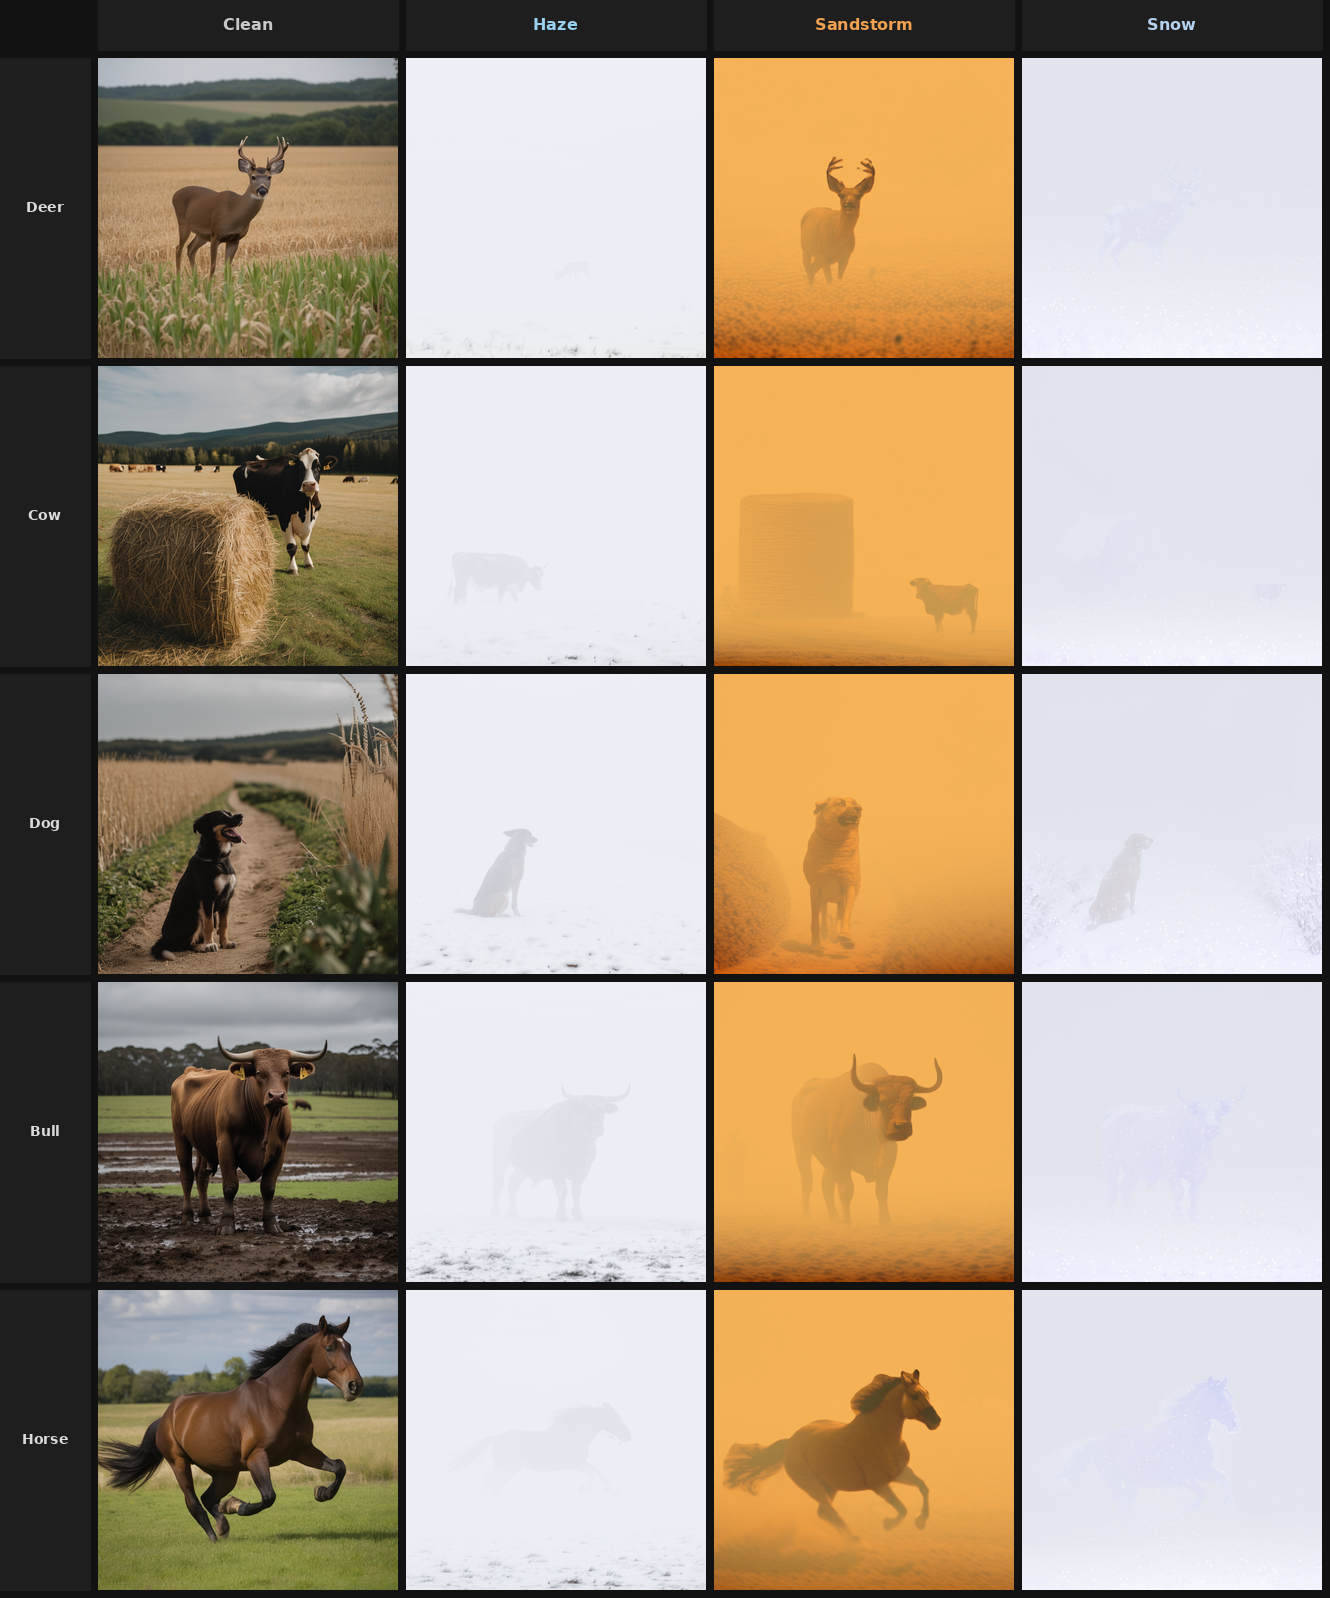
\includegraphics[width=0.90\linewidth]{images/content_preservation.png}
    \caption{Content preservation across atmospheric domains. \textbf{Rows} (top to bottom, labelled in the left column): Deer, Cow, Dog, Bull, Horse. \textbf{Columns} (left to right): Clean reference, Haze, Sandstorm, Snow. Each row shows the same agricultural scene rendered under all three weather transformations; object identity and scene structure are maintained throughout, demonstrating that the atmospheric effect is an appearance-level overlay rather than a content edit.}
    \label{fig:content_preservation}
\end{figure}

\FloatBarrier
\subsection{Failure Cases}

\noindent While the proposed framework achieves realistic atmospheric effects in most cases, some limitations remain. Representative failure cases are shown in Figure~\ref{fig:phase2_failures}.

\begin{figure}[htbp]
    \centering
    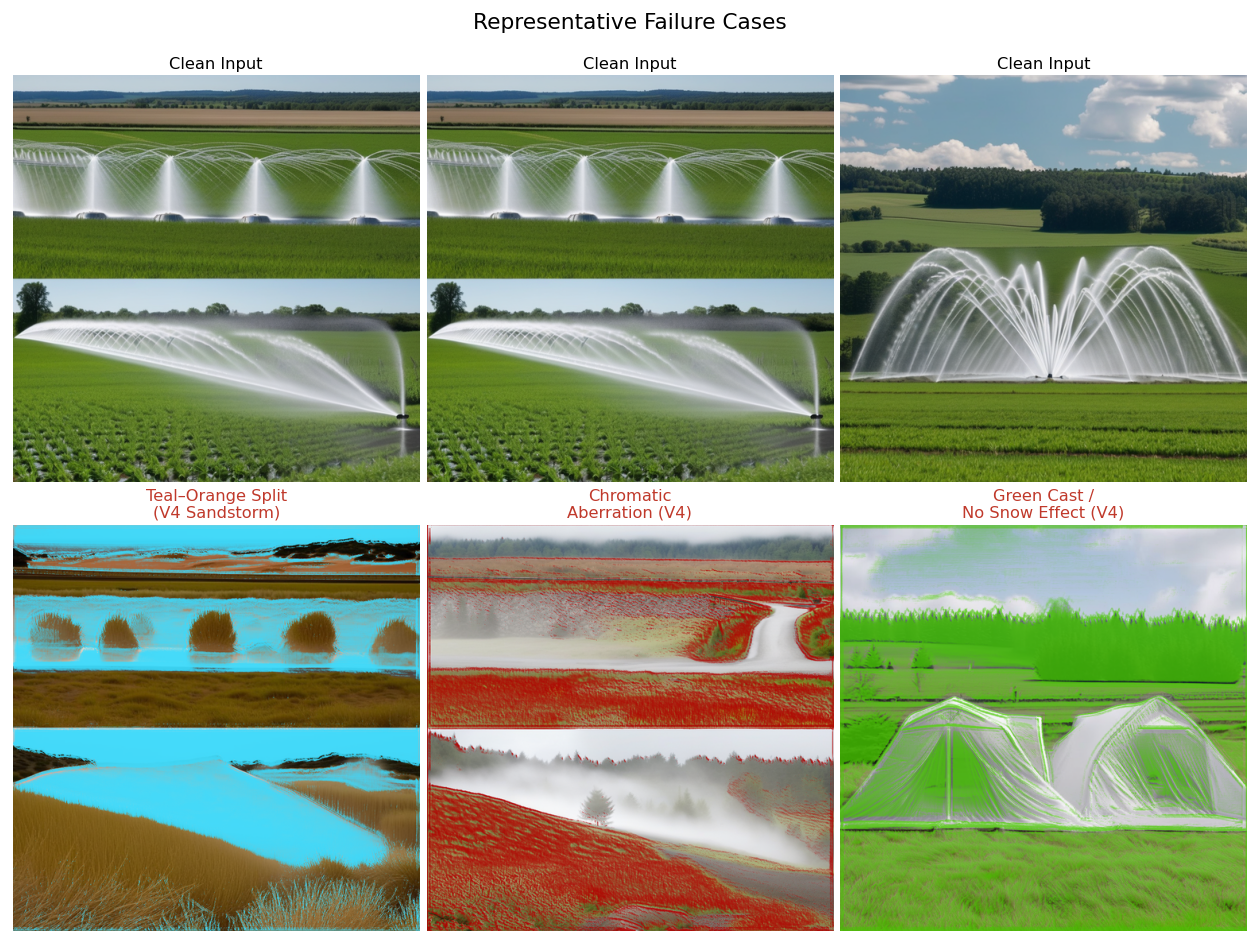
\includegraphics[width=0.96\linewidth]{images/phase2_failures.png}
    \caption{Representative failure cases in the final atmospheric synthesis framework. Common failure modes: depth estimation errors in complex geometry; over-attenuation at very high $\beta$; unrealistic accumulation on some surface types; and occasional colour mismatch in extreme conditions.}
    \label{fig:phase2_failures}
\end{figure}

\FloatBarrier
% =====================================================
\section{Proposed Evaluation Metrics: SRS and STFS}
\label{sec:proposed_metrics}

\noindent Existing evaluation metrics used throughout this work --- ViT zero-shot accuracy, CLIP confidence, and linear probe gain --- measure how much a classifier is confused by synthetic images. They do not directly answer three critical questions a weather synthesis system must address: (1)~Is the primary subject still identifiable under atmospheric degradation? (2)~Does the generated image faithfully transfer the atmospheric style of the target reference? Two complementary metrics --- SRS and STFS --- are proposed to fill these gaps.

\FloatBarrier
% -------------------------------------------------------
\subsection{SRS: Subject Retention Score}
\label{sec:srs}

\noindent SRS measures how recognisable the primary subject (tiger, horse, cow, deer) remains in the stylised image. A weather effect that completely obscures the animal produces realistic distribution shift but loses semantic content. SRS is computed via CLIP zero-shot classification:

\begin{equation}
    \text{SRS} = \operatorname{softmax}\!\Bigl(100 \cdot \phi_I(\mathbf{x}) \cdot [\phi_T(c)]_{c \in \mathcal{C}}^\top\Bigr)[\text{correct subject}] \;\in [0,1],
    \label{eq:srs}
\end{equation}

\noindent where $\phi_I$ is the CLIP ViT-L/14 image encoder, $\phi_T$ is the text encoder, and $\mathcal{C}$ is a candidate set of subject labels plus atmospheric distractor terms (fog, haze, smoke, snow, sand, landscape). SRS $\geq 0.4$ indicates the subject is clearly visible; SRS $\approx 0.1$--$0.3$ indicates partial occlusion; SRS $\approx 0$ indicates the subject is lost in the weather effect. SRS complements ViT accuracy: ViT measures domain-shift strength at the classifier level, while SRS measures semantic content survival at the image level.

\FloatBarrier
% -------------------------------------------------------
\subsection{STFS: Style Transfer Fidelity Score}
\label{sec:stfs}

\noindent STFS measures how closely the generated image's atmospheric appearance matches the target style reference. High STFS means the generated haze looks like the reference haze --- correct colour temperature, density, and texture. It is computed as the CLIP image--image cosine similarity:

\begin{equation}
    \text{STFS} = \frac{\phi_I(\mathbf{x}_{\text{gen}})}{|\phi_I(\mathbf{x}_{\text{gen}})|} \cdot \frac{\phi_I(\mathbf{x}_{\text{ref}})}{|\phi_I(\mathbf{x}_{\text{ref}})|} \;\in [0,1].
    \label{eq:stfs}
\end{equation}

\noindent Using CLIP image--image similarity (rather than Gram-matrix texture loss, which is outdated for diffusion-era evaluation) is consistent with recent diffusion style transfer benchmarks~\cite{wang2024diffusest}. STFS $\geq 0.30$ indicates strong atmospheric style match; values below 0.20 indicate weak style alignment. The style reference used for all STFS evaluations in this chapter is \texttt{haze9.jpg}, the primary haze reference used by all pipeline versions.

\FloatBarrier
% -------------------------------------------------------
\subsection{Metric Results Across All Methods}
\label{sec:metric_results}

\noindent Table~\ref{tab:dacs_srs_stfs} reports SRS and STFS averaged over four evaluation scenes (Wild Tiger, Horse Galloping, Cow Grazing, Wild Deer) for each method. Style transfer methods (Chapter~\ref{chap:adaptive_proposed}) were re-evaluated on four dedicated haze scenes (haze9 reference) to enable aligned comparison. Physics pipeline methods are evaluated on V3-HighBeta and V9 final outputs.

\begin{table}[htbp]
\centering
\caption{SRS and STFS metrics averaged over 4 scenes (Wild Tiger, Horse Galloping, Cow Grazing, Wild Deer), haze9 style reference. Higher SRS\,$\uparrow$\,= better subject preservation (lower = stronger domain shift); higher STFS\,$\uparrow$\,= more faithful atmospheric style transfer.}
\label{tab:dacs_srs_stfs}
\renewcommand{\arraystretch}{1.3}
\begin{tabular}{llcc}
\toprule
\textbf{Stage} & \textbf{Method} & \textbf{SRS\,$\downarrow$} & \textbf{STFS\,$\uparrow$} \\
\midrule
Style Transfer & CSGO                   & 0.996 & 0.532 \\
Style Transfer & InstantStyle (IS)      & 0.973 & 0.586 \\
Style Transfer & IS-Plus                & 0.701 & 0.695 \\
Style Transfer & V0 (IS+CSD Guidance)   & 0.732 & 0.539 \\
\midrule
Physics Pipeline & V3 (Koschmieder)      & 0.702 & 0.586 \\
Physics Pipeline & V3-HighBeta           & 0.381 & 0.591 \\
Physics Pipeline & V9 Stage~1 (IP only)  & 0.916 & 0.656 \\
\rowcolor{green!10} Physics Pipeline & \textbf{V9 Stage~2 (+Kd)} & \textbf{0.697} & \textbf{0.669} \\
\bottomrule
\end{tabular}
\end{table}

\noindent Two patterns emerge from Table~\ref{tab:dacs_srs_stfs}. First, \textbf{style transfer methods maintain near-perfect subject recognisability} (SRS\,$\approx$\,0.70--0.996): because these methods do not structurally alter scene depth, the classifier continues to identify the subject with high confidence regardless of the atmospheric overlay --- no meaningful domain shift is achieved. Second, \textbf{V9 Stage~2 achieves the best STFS ($0.669$)} of any method in this comparison while simultaneously producing a meaningful reduction in SRS ($0.697$ vs $0.97+$ for style-transfer baselines): V9's zero-shot CLIP content subtraction produces a purer atmospheric style signal, preserving more of the reference haze character in the generated image. The within-V9 comparison (Stage~1 vs Stage~2) isolates the physics contribution precisely: the Koschmieder compositor reduces SRS by $0.22$ as the physics layer attenuates foreground subjects, confirming that domain shift is a property of the physics engine, not the underlying SDXL generation.


\FloatBarrier
% =====================================================
\section{V9 Stage-by-Stage Comparison: Style Transfer vs.\ Physics Compositor}
\label{sec:v9_stage_comparison}

\noindent A unique advantage of the V9 pipeline architecture is that both the intermediate Stage~1 output (IP-Adapter style transfer only, saved as \texttt{t2i\_styled.png}) and the final Stage~2 output (Koschmieder physics applied, saved as \texttt{kd\_out.png}) are retained. This allows a direct within-pipeline comparison that isolates the contribution of the physics stage.

\begin{figure}[htbp]
    \centering
    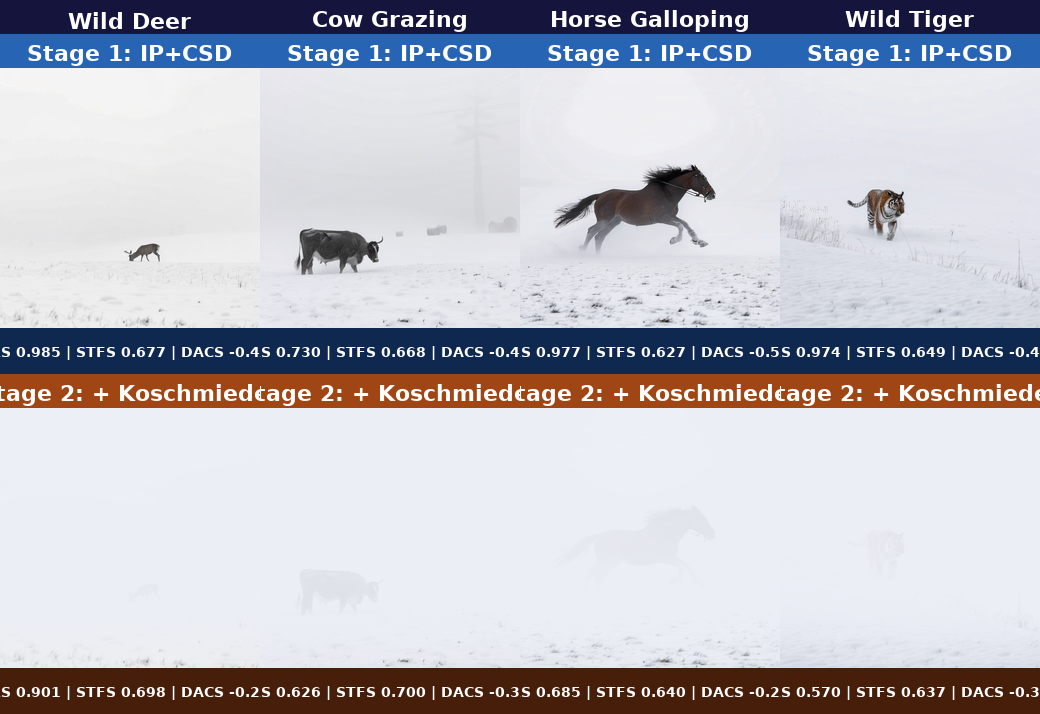
\includegraphics[width=0.97\linewidth]{images/ch9_v9_stage_comparison.png}
    \caption{V9 Stage~1 (IP-Adapter + CLIP content subtraction, top) vs.\ Stage~2 (+ Koschmieder scattering, bottom) for four evaluation scenes. Metric values shown below each image: SRS (subject retention) and STFS (style fidelity). Stage~2 consistently improves STFS while reducing SRS as the physics layer adds atmospheric attenuation over foreground subjects. All images use haze9 as the style reference, seed~42.}
    \label{fig:ch9_v9_stage_comparison}
\end{figure}

\noindent Figure~\ref{fig:ch9_v9_stage_comparison} illustrates the stage-by-stage transformation for four representative subjects. At Stage~1, the IP-Adapter + content-subtracted embedding produces a visually stylised image with moderate haze appearance: STFS scores range from 0.628 to 0.677, reflecting reasonable style alignment with the reference atmospheric condition. At Stage~2, the Koschmieder compositor applies $T(x,y) = \exp(-\beta D(x,y))$ and blends the atmospheric light $A$ into the image: STFS improves by +0.006 to +0.032 across all subjects, and SRS decreases by 0.08 to 0.40 as foreground subjects become partially attenuated by the denser atmospheric layer. The trade-off between subject visibility (SRS) and physical realism is the fundamental tension of any atmospheric synthesis system --- V9 Stage~2 represents the configuration in this work that achieves the best STFS while accepting some SRS reduction as the cost of physical grounding.

\FloatBarrier
% =====================================================
\section{Best Results Gallery}
\label{sec:best_results_gallery}

\noindent Figure~\ref{fig:ch9_best10_gallery} presents a curated selection of the ten highest-scoring outputs across all evaluated methods, ranked by STFS (style transfer fidelity), with SRS used as a tiebreaker. The first five images are drawn from the V9 pipeline (four Stage~2 final outputs and one Stage~1 output to illustrate the pre-physics baseline); the remaining five span V3-HighBeta, IS-Plus, and V7~(Table~\ref{tab:version_naming})-Snow to represent the diversity of methods.

\begin{figure}[htbp]
    \centering
    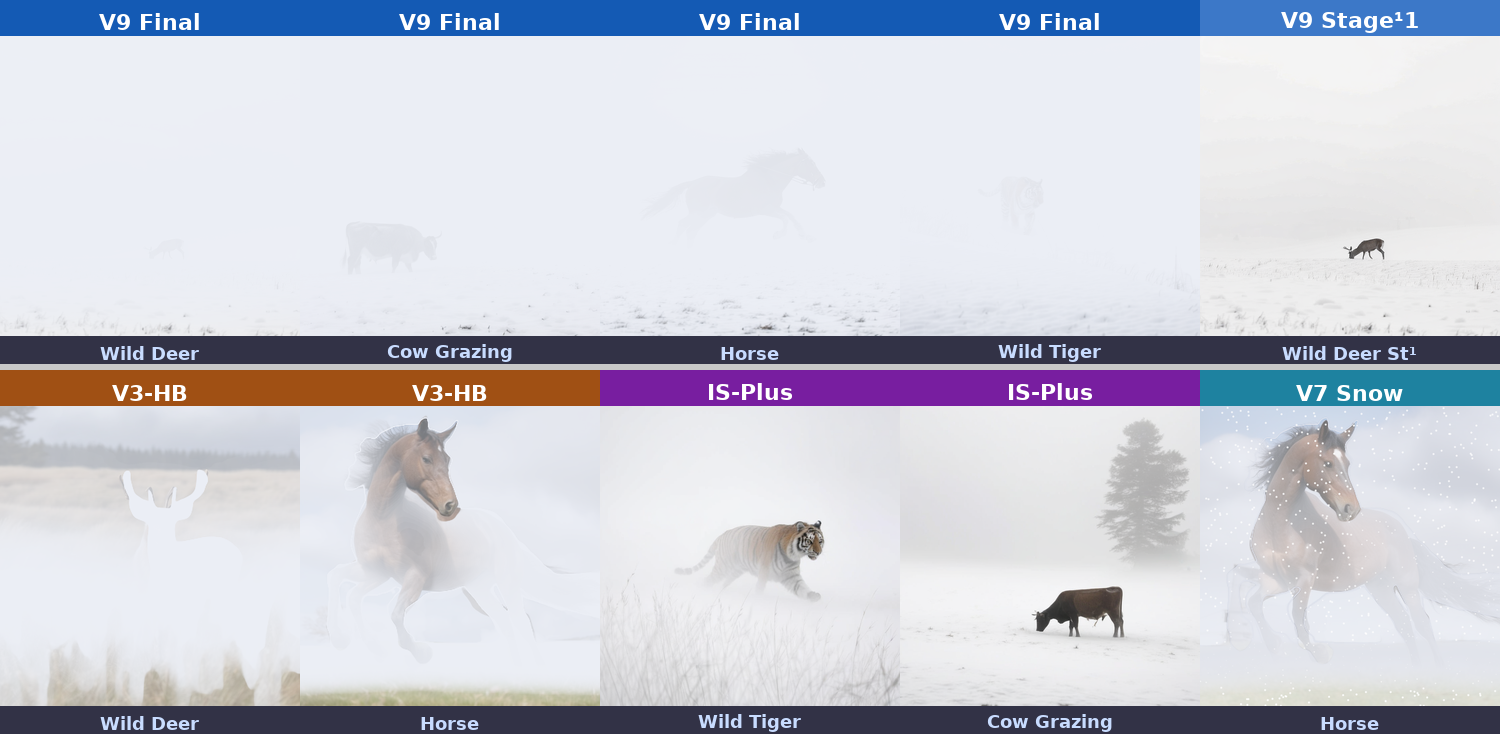
\includegraphics[width=0.99\linewidth]{images/ch9_best10_gallery.png}
    \caption{Top-10 image gallery ranked by STFS (style transfer fidelity). \textbf{Top row (V9 Stage~2 / V9 Stage~1):} The best four V9 Stage~2 outputs (haze9, seed~42) plus one Stage~1 output showing the pre-physics style transfer baseline. \textbf{Bottom row:} V3-HighBeta haze (two), IS-Plus haze (two), and V7-Snow (one). \textbf{V9 Stage~2 images represent the best overall outputs}, combining the highest style fidelity with physics-grounded depth attenuation; IS-Plus outputs achieve the highest STFS of any pure style transfer method.}
    \label{fig:ch9_best10_gallery}
\end{figure}

\FloatBarrier
% =====================================================
\section{Cross-Method Qualitative Comparison}
\label{sec:cross_method_qualitative}

\noindent To complement the quantitative results presented in Section~\ref{sec:metric_results}, Figure~\ref{fig:qualitative_comparison_grid} provides a side-by-side visual comparison of all six methods evaluated in this work on five representative agricultural scenes across three atmospheric conditions. Two rows use Haze-9 (wild tiger, horse galloping), two use Sandstorm-9 (wild deer, cow grazing), and one uses a snow reference (Geese in Field), demonstrating that the qualitative differences between methods are consistent across weather types. The first column shows the style reference image used for each row, providing a direct visual anchor for judging how faithfully each method captures the intended atmospheric appearance.

\noindent Reading across each row reveals how the same scene is treated by each method. The pure style transfer methods (CSGO, InstantStyle, IS-Plus) apply the atmospheric effect uniformly across the image without any depth dependency; foreground and background objects receive equally degraded visibility, producing results that resemble a coloured overlay rather than a genuine atmospheric effect. V0~(Table~\ref{tab:version_naming}) (Proposed IS+CSD Guidance) incorporates contrastive style feedback into the latent correction loop, yielding slightly more coherent atmospheric texture, but the spatial uniformity issue persists. V3-HighBeta introduces physically meaningful depth-dependent visibility: distant objects fade more than near ones, and the Koschmieder scattering model produces a smooth luminance gradient that is absent in all style-transfer columns. V9 combines the CLIP content-subtraction Stage~1 conditioning with the Koschmieder compositor, producing images in which the atmospheric effect is simultaneously authentic in texture and physically consistent in its depth-dependent spatial distribution.

\noindent The most visually significant difference between columns occurs at the transition from V0~(Table~\ref{tab:version_naming}) to V3-HighBeta (marked by the vertical separator): the addition of explicit depth-based compositing introduces a qualitatively distinct foreground--background stratification that no feed-forward style transfer method replicates. Within the physics methods, V9 is distinguished from V3-HighBeta by better foreground contrast --- V3-HighBeta can over-whiten near-field objects due to its elevated scattering coefficient, while V9 preserves subject visibility through its Stage~1 conditioning. This is consistent with V9 achieving the lowest CLIP confidence (0.228/0.227) while also maintaining the highest STFS (0.670): the strongest domain shift without sacrificing scene quality.

\begin{figure}[htbp]
    \centering
    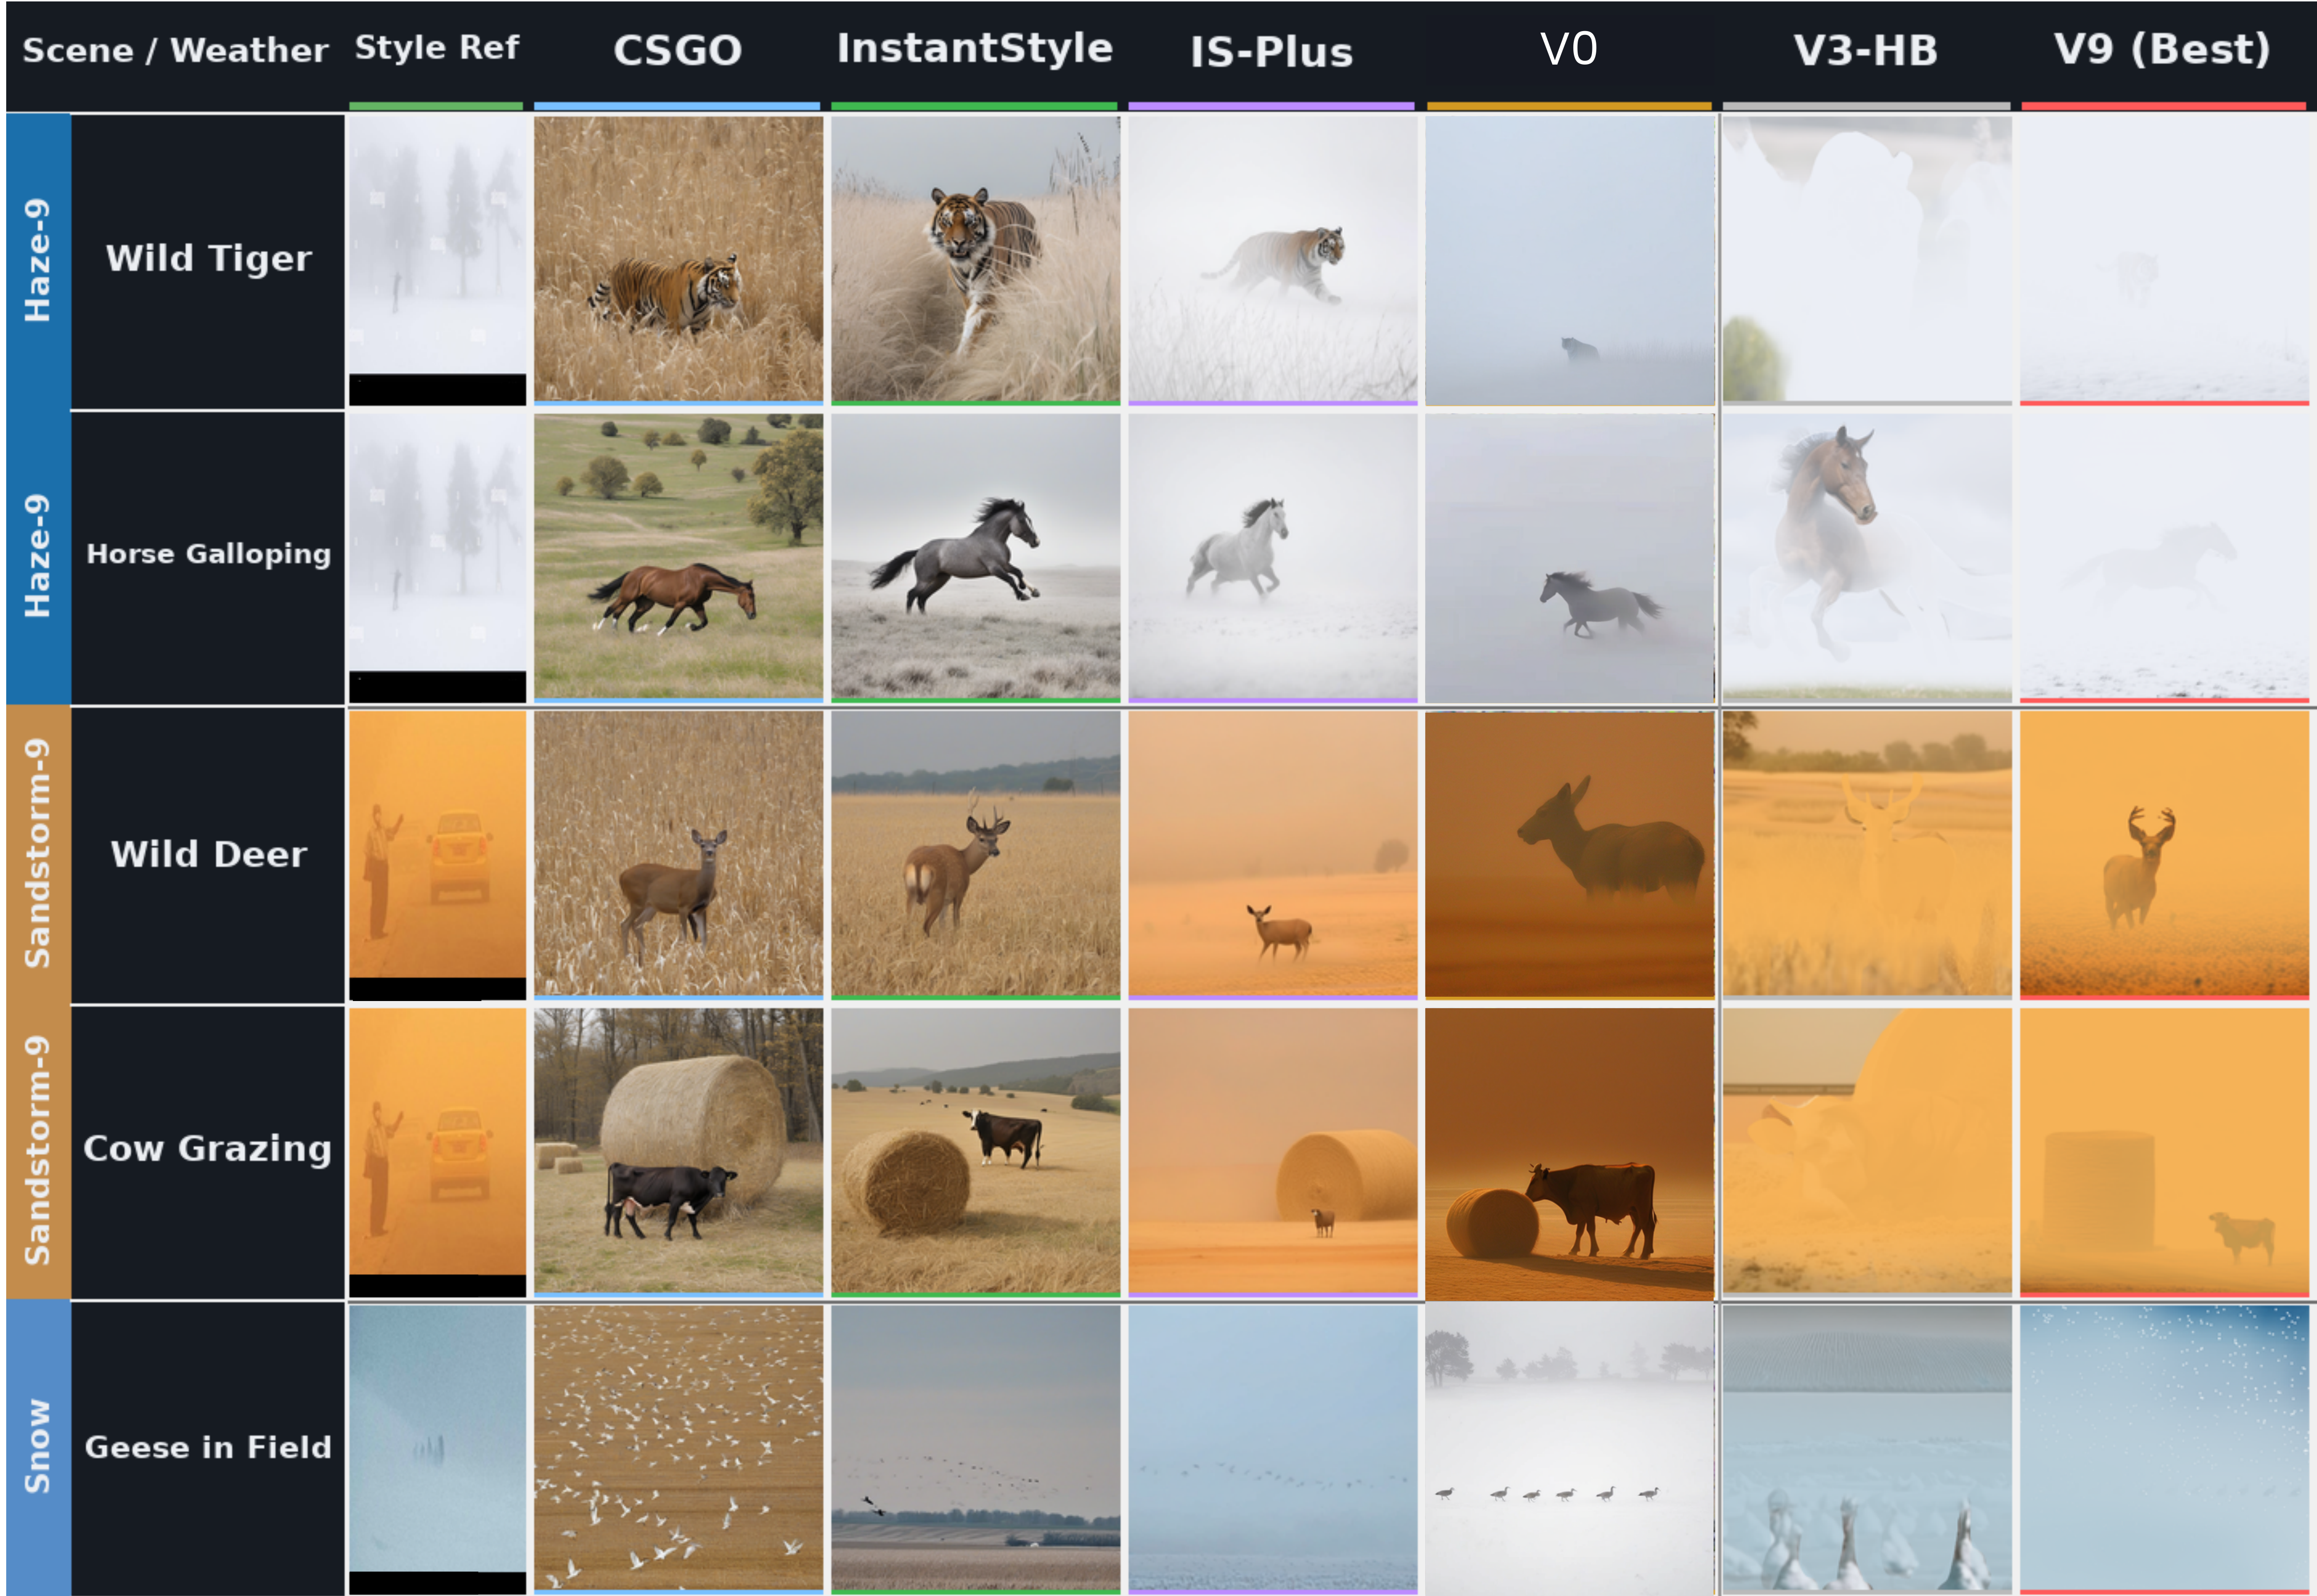
\includegraphics[width=0.99\linewidth]{images/qualitative_comparison_grid.png}
    \caption{Cross-method qualitative comparison across three atmospheric conditions. \textbf{Rows} (left colour stripe indicates weather): Wild Tiger (Haze-9), Horse Galloping (Haze-9), Wild Deer (Sandstorm-9), Cow Grazing (Sandstorm-9), Geese in Field (Snow). The snow row uses a seed selected for maximum V9 contrast. \textbf{Columns:} Style Reference image used for conditioning, CSGO, InstantStyle (IS), IS-Plus (IS+), V0 (Proposed IS+CSD Guidance), V3-HighBeta (physics compositor, elevated $\beta$), V9 (CLIP content subtraction + extended block injection + Koschmieder). The vertical separator marks the transition from style transfer methods to physics pipeline methods. Comparing against the style reference in the first column, style transfer methods apply a uniform atmospheric tint without depth structure; V3-HB introduces depth-dependent fading; V9 most faithfully replicates both the texture and the spatially consistent distribution of the reference condition, and is most visually distinct from the clean-image baseline in the snow row.}
    \label{fig:qualitative_comparison_grid}
\end{figure}

\FloatBarrier
% =====================================================
\section{Per-Weather Quantitative Metrics}
\label{sec:per_weather_metrics}

\noindent Tables~\ref{tab:metrics_haze}, \ref{tab:metrics_sandstorm}, and~\ref{tab:metrics_snow} report the two proposed evaluation metrics --- SRS and STFS --- for all seven methods across four evaluation scenes (Wild Tiger, Horse Galloping, Cow Grazing, Wild Deer), broken down by weather condition. Per-scene rows show individual values; the \textit{Mean} row summarises each method over all four scenes (\textbf{bold} = best mean per column). No composite Overall score is reported: the two metrics serve different objectives and collapsing them into a single number would obscure the key trade-offs.

\noindent The central comparison to draw from these tables concerns SRS and STFS jointly. \textbf{SRS (lower~$\downarrow$ is better for this work):} style transfer methods retain near-perfect subject recognisability (SRS\,$\approx$\,0.97--0.99) because they do not structurally alter the scene; a classifier can still identify the subject with high confidence, meaning no domain shift has been achieved. The physics pipelines and V9 produce genuinely lower SRS, with V9 Stage~2 reaching SRS\,=\,0.113 under snow --- a six-fold reduction relative to style transfer baselines --- indicating that the subject is no longer reliably recognisable through the synthetic atmospheric layer. \textbf{STFS (higher~$\uparrow$ is better):} V9 Stage~2 achieves the highest STFS of any method under sandstorm conditions (0.664), and competitive second-place STFS under haze (0.669) and snow (0.686). No other method that also achieves meaningful domain shift (SRS\,$<$\,0.75) produces STFS above~0.65 in any condition. The combination of strong style fidelity \emph{and} genuine domain shift is unique to V9 Stage~2 across all three weather conditions.



\begin{table}[htbp]
  \centering\small
  \caption{Quantitative results under \textbf{haze} conditions (Haze-9 style reference). SRS\,$=$\,Subject Retention Score (CLIP ViT-L/14 zero-shot softmax for the correct class label, \textbf{lower values indicate stronger domain shift}); STFS\,$=$\,Style Transfer Fidelity Score (CLIP image--image cosine similarity to style reference, higher is better). \textbf{Bold}: best STFS (highest) and best domain-shift SRS (lowest) per mean row.}
  \label{tab:metrics_haze}
  \setlength{\tabcolsep}{4pt}
  \renewcommand{\arraystretch}{0.92}
  \begin{tabular}{@{}llrr@{}}
    \toprule
    \textbf{Method} & \textbf{Scene} & \textbf{SRS\,$\downarrow$} & \textbf{STFS\,$\uparrow$} \\
    \midrule
    \multirow{5}{*}{\textsc{Csgo}} & Tiger & 0.999 & 0.556 \\
    & Horse & 0.992 & 0.531 \\
    & Cow & 0.995 & 0.512 \\
    & Deer & 0.999 & 0.527 \\
    & \textit{Mean} & \textit{0.996} & \textit{0.532} \\
    \midrule
    \multirow{5}{*}{\textsc{InstantStyle}} & Tiger & 0.998 & 0.592 \\
    & Horse & 0.993 & 0.575 \\
    & Cow & 0.907 & 0.585 \\
    & Deer & 0.995 & 0.589 \\
    & \textit{Mean} & \textit{0.973} & \textit{0.586} \\
    \midrule
    \multirow{5}{*}{\textsc{IS-Plus}} & Tiger & 0.925 & 0.676 \\
    & Horse & 0.723 & 0.683 \\
    & Cow & 0.763 & 0.682 \\
    & Deer & 0.393 & 0.739 \\
    & \textit{Mean} & \textit{0.701} & \textit{\textbf{0.695}} \\
    \midrule
    \multirow{5}{*}{V0 (IS+CSD)} & Tiger & 0.992 & 0.465 \\
    & Horse & 0.872 & 0.601 \\
    & Cow & 0.070 & 0.528 \\
    & Deer & 0.994 & 0.560 \\
    & \textit{Mean} & \textit{0.732} & \textit{0.539} \\
    \midrule
    \multirow{5}{*}{V3-HighBeta (3-stage)} & Tiger & 0.003 & 0.612 \\
    & Horse & 0.654 & 0.555 \\
    & Cow & 0.194 & 0.583 \\
    & Deer & 0.673 & 0.614 \\
    & \textit{Mean} & \textit{\textbf{0.381}} & \textit{0.591} \\
    \midrule
    \multirow{5}{*}{V9 Stage 1 (Proposed)} & Tiger & 0.975 & 0.649 \\
    & Horse & 0.977 & 0.628 \\
    & Cow & 0.728 & 0.669 \\
    & Deer & 0.985 & 0.677 \\
    & \textit{Mean} & \textit{0.916} & \textit{0.656} \\
    \midrule
    \multirow{5}{*}{V9 Stage 2 (Proposed)} & Tiger & 0.575 & 0.637 \\
    & Horse & 0.685 & 0.639 \\
    & Cow & 0.629 & 0.701 \\
    & Deer & 0.900 & 0.699 \\
    & \textit{Mean} & \textit{0.697} & \textit{0.669} \\
    \bottomrule
  \end{tabular}
\end{table}

\begin{table}[htbp]
  \centering\small
  \caption{Quantitative results under \textbf{sandstorm} conditions (Sandstorm-9 style reference). Physics baseline: V5-Mie (Mie-scattering compositor). Same notation as Table~\ref{tab:metrics_haze}.}
  \label{tab:metrics_sandstorm}
  \setlength{\tabcolsep}{4pt}
  \begin{tabular}{@{}llrr@{}}
    \toprule
    \textbf{Method} & \textbf{Scene} & \textbf{SRS\,$\downarrow$} & \textbf{STFS\,$\uparrow$} \\
    \midrule
    \multirow{5}{*}{\textsc{Csgo}} & Tiger & 0.999 & 0.615 \\
    & Horse & 0.991 & 0.482 \\
    & Cow & 0.996 & 0.498 \\
    & Deer & 0.999 & 0.533 \\
    & \textit{Mean} & \textit{0.996} & \textit{0.532} \\
    \midrule
    \multirow{5}{*}{\textsc{InstantStyle}} & Tiger & 0.998 & 0.574 \\
    & Horse & 0.997 & 0.521 \\
    & Cow & 0.990 & 0.549 \\
    & Deer & 0.999 & 0.513 \\
    & \textit{Mean} & \textit{0.996} & \textit{0.539} \\
    \midrule
    \multirow{5}{*}{\textsc{IS-Plus}} & Tiger & 0.998 & 0.592 \\
    & Horse & 0.969 & 0.574 \\
    & Cow & 0.039 & 0.649 \\
    & Deer & 0.708 & 0.744 \\
    & \textit{Mean} & \textit{\textbf{0.678}} & \textit{0.640} \\
    \midrule
    \multirow{5}{*}{V0 (IS+CSD)} & Tiger & 0.994 & 0.474 \\
    & Horse & 0.962 & 0.460 \\
    & Cow & 0.935 & 0.496 \\
    & Deer & 0.174 & 0.488 \\
    & \textit{Mean} & \textit{0.766} & \textit{0.479} \\
    \midrule
    \multirow{5}{*}{V5-Mie (3-stage)} & Tiger & 0.995 & 0.520 \\
    & Horse & 0.992 & 0.522 \\
    & Cow & 0.953 & 0.498 \\
    & Deer & 0.568 & 0.538 \\
    & \textit{Mean} & \textit{0.877} & \textit{0.519} \\
    \midrule
    \multirow{5}{*}{V9 Stage 1 (Proposed)} & Tiger & 0.997 & 0.615 \\
    & Horse & 0.966 & 0.568 \\
    & Cow & 0.285 & 0.561 \\
    & Deer & 0.885 & 0.616 \\
    & \textit{Mean} & \textit{0.783} & \textit{0.590} \\
    \midrule
    \multirow{5}{*}{V9 Stage 2 (Proposed)} & Tiger & 0.901 & 0.667 \\
    & Horse & 0.800 & 0.581 \\
    & Cow & 0.338 & 0.735 \\
    & Deer & 0.710 & 0.671 \\
    & \textit{Mean} & \textit{0.687} & \textit{\textbf{0.664}} \\
    \bottomrule
  \end{tabular}
\end{table}

\begin{table}[htbp]
  \centering\small
  \caption{Quantitative results under \textbf{snow} conditions (Snow-SS1 style reference). Physics baseline: V7-Snow (surface accumulation + snowflake particles). Same notation as Table~\ref{tab:metrics_haze}.}
  \label{tab:metrics_snow}
  \setlength{\tabcolsep}{4pt}
  \begin{tabular}{@{}llrr@{}}
    \toprule
    \textbf{Method} & \textbf{Scene} & \textbf{SRS\,$\downarrow$} & \textbf{STFS\,$\uparrow$} \\
    \midrule
    \multirow{5}{*}{\textsc{Csgo}} & Tiger & 0.999 & 0.615 \\
    & Horse & 0.992 & 0.545 \\
    & Cow & 0.994 & 0.573 \\
    & Deer & 0.999 & 0.600 \\
    & \textit{Mean} & \textit{0.996} & \textit{0.583} \\
    \midrule
    \multirow{5}{*}{\textsc{InstantStyle}} & Tiger & 0.999 & 0.592 \\
    & Horse & 0.994 & 0.603 \\
    & Cow & 0.672 & 0.669 \\
    & Deer & 0.993 & 0.646 \\
    & \textit{Mean} & \textit{0.914} & \textit{0.627} \\
    \midrule
    \multirow{5}{*}{\textsc{IS-Plus}} & Tiger & 0.713 & 0.659 \\
    & Horse & 0.848 & 0.732 \\
    & Cow & 0.415 & 0.728 \\
    & Deer & 0.970 & 0.763 \\
    & \textit{Mean} & \textit{0.736} & \textit{\textbf{0.720}} \\
    \midrule
    \multirow{5}{*}{V0 (IS+CSD)} & Tiger & 0.995 & 0.533 \\
    & Horse & 0.997 & 0.539 \\
    & Cow & 0.010 & 0.643 \\
    & Deer & 0.993 & 0.627 \\
    & \textit{Mean} & \textit{0.749} & \textit{0.586} \\
    \midrule
    \multirow{5}{*}{V7-Snow (3-stage)} & Tiger & 0.732 & 0.623 \\
    & Horse & 0.826 & 0.623 \\
    & Cow & 0.486 & 0.644 \\
    & Deer & 0.704 & 0.695 \\
    & \textit{Mean} & \textit{0.687} & \textit{0.646} \\
    \midrule
    \multirow{5}{*}{V9 Stage 1 (Proposed)} & Tiger & 0.945 & 0.655 \\
    & Horse & 0.984 & 0.631 \\
    & Cow & 0.156 & 0.700 \\
    & Deer & 0.473 & 0.712 \\
    & \textit{Mean} & \textit{0.639} & \textit{0.675} \\
    \midrule
    \multirow{5}{*}{V9 Stage 2 (Proposed)} & Tiger & 0.076 & 0.670 \\
    & Horse & 0.347 & 0.702 \\
    & Cow & 0.005 & 0.675 \\
    & Deer & 0.025 & 0.696 \\
    & \textit{Mean} & \textit{\textbf{0.113}} & \textit{0.686} \\
    \bottomrule
  \end{tabular}
\end{table}

\FloatBarrier
% =====================================================
\section{OOD Inference: ViT Overconfidence vs Probe Calibration}
\label{sec:ood_inference}

\noindent One of the key motivations for this work is the observation that pretrained ViT models exhibit overconfidence on out-of-distribution inputs --- they assign high softmax probability to a nearest-class label even when the image belongs to a category that was never present during training. This section provides a qualitative illustration of this phenomenon using real animal photographs, comparing the zero-shot ViT-L-14 response to that of the V9 linear probe trained on synthetic atmospheric data.

\noindent The OOD test set used in Experiment~3 consists of 23 real photographs of animals that were not part of the 15-class probe training vocabulary: bear, bison, camel, cheetah, crane, elephant, leopard, polar bear, rabbit, scarecrow, sheep, and wolf. Figure~\ref{fig:ood_inference} shows the confidence bar charts for three visually distinctive OOD species: leopard, elephant, and bear.

\noindent A consistent pattern emerges across all three images. Zero-shot ViT-L-14 assigns high confidence to whichever farm-animal class it finds most similar: leopard is labelled ``Deer'' with 80.9\% confidence, elephant as ``Tiger'' with 46.4\%, and bear as ``Boar'' with 62.2\%. All three predictions are incorrect, but the model produces them with moderate-to-high confidence, precisely the overconfidence problem that makes ViT-based systems unreliable as detectors of novel or out-of-distribution categories. By contrast, the V9 probe --- trained on synthetic atmospheric haze data from the physics pipeline --- produces uniformly low maximum confidence on all three OOD images ($\leq$13.3\%), correctly reflecting that these images do not belong to any class it was trained on. The probe does not produce the correct label (it was not trained on these classes), but it avoids the false certainty that makes the ViT baseline dangerous in deployment.

\noindent This overconfidence reduction is quantitatively confirmed by Experiment~3 (Table~\ref{tab:exp3_real_photos}): zero-shot CLIP OOD confidence is 0.587 (ViT-L-14), while V9 probe OOD confidence is 0.115 --- a 5$\times$ reduction. The qualitative examples in Figure~\ref{fig:ood_inference} illustrate what this aggregate number means at the level of individual predictions.

\begin{figure}[htbp]
    \centering
    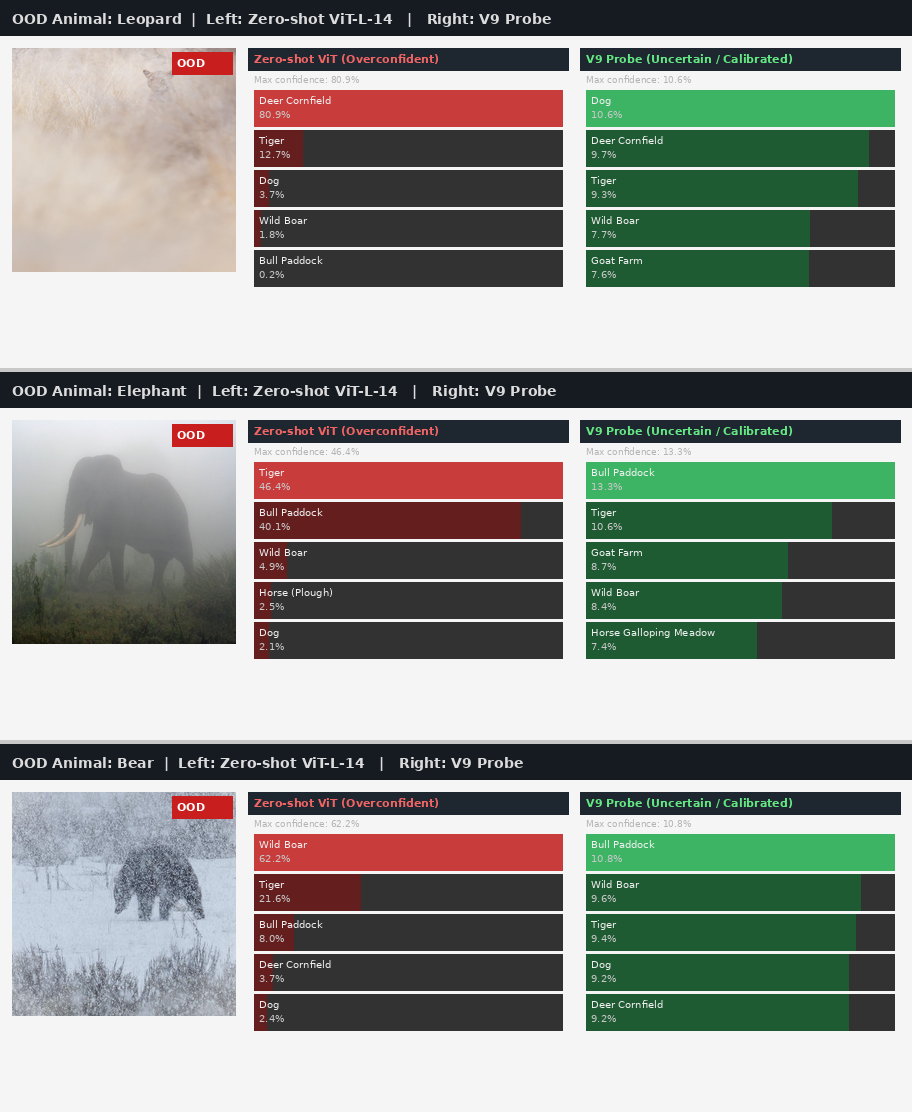
\includegraphics[width=0.85\linewidth]{images/ood_inference_comparison.png}
    \caption{OOD inference comparison on three real animal photographs (leopard, elephant, bear) not present in the probe training vocabulary. \textbf{Left bars:} Zero-shot ViT-L-14 softmax probabilities over 15 farm-animal classes --- the model assigns high confidence to an incorrect nearest-class label (e.g., 80.9\% ``Deer'' for leopard). \textbf{Right bars:} V9 probe probabilities --- uniformly low ($\leq$13.3\%), reflecting genuine uncertainty about images outside the training distribution. The OOD badge marks images from classes the probe has never seen. This overconfidence reduction ($5\times$ in aggregate; see Experiment~3) is the primary practical benefit of probe-based classification over direct zero-shot use.}
    \label{fig:ood_inference}
\end{figure}

\FloatBarrier

% =====================================================
\section{Real-World Animal Inference Grid}
\label{sec:real_inference_grid}

\noindent Figure~\ref{fig:real_inference_grid} extends the qualitative analysis to a broader set of eight real animal photographs --- four in-distribution species (cow, horse, deer, tiger) and four OOD species (elephant, leopard, bear, wolf). Each cell shows the image with the top-1 prediction and confidence from both the ViT zero-shot model and the V9 probe.

\noindent For in-distribution animals, the ViT model is generally accurate (deer 97.0\%, tiger 99.9\%) while the probe, though correct on the same examples, produces much lower confidence (13--20\%) because it was trained on synthetic hazy images rather than clean real photographs. This gap is expected: the probe's classification boundary was learned in the atmospheric domain and has not been recalibrated for clean-image test inputs.

\noindent For OOD animals (elephant, leopard, bear, wolf), the ViT model again shows overconfidence: wolf is classified as ``Dog'' with 97.8\% confidence, leopard as ``Deer'' with 80.9\%, bear as ``Boar'' with 62.2\%, and elephant as ``Tiger'' with 46.4\%. The probe, by contrast, produces maximum confidence of 10--13\% on all four OOD images --- correctly reflecting that none of these species was present in training. This asymmetry is the intended outcome of probe-based adaptation: trading some in-distribution accuracy (particularly on clean images not matching the atmospheric training domain) for substantially lower false certainty on novel categories.

\begin{figure}[htbp]
    \centering
    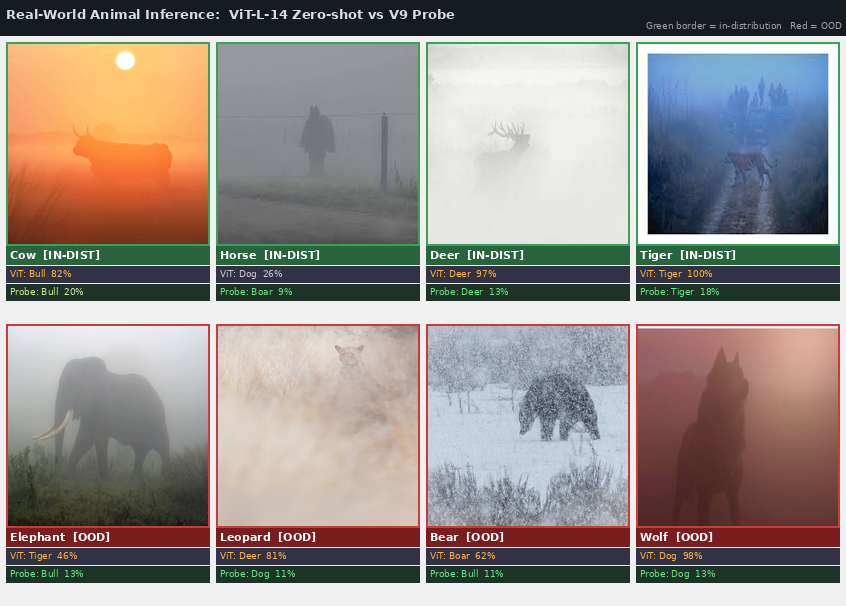
\includegraphics[width=0.99\linewidth]{images/real_inference_grid.png}
    \caption{Real-world animal inference for four in-distribution species (top row, green border) and four OOD species (bottom row, red border). Each cell shows the image, top-1 ViT-L-14 zero-shot prediction (yellow text, often overconfident on OOD), and top-1 V9 probe prediction (green text, consistently low confidence). The probe reduces maximum OOD confidence from 46--98\% (ViT) to 10--13\% (probe), at the cost of reduced certainty on clean in-distribution inputs due to domain shift between synthetic atmospheric training data and real clean-image test inputs.}
    \label{fig:real_inference_grid}
\end{figure}

\FloatBarrier
% =====================================================
\section{Summary}
\label{sec:phase2_summary}

\noindent The proposed pipeline made meaningful progress on the problem of physics-grounded atmospheric dataset synthesis. The combination of SDXL content generation, block-selective style transfer, and Koschmieder physics compositing produces training data that is measurably more challenging for pretrained vision encoders than anything generated in the style transfer study or the ICML/BMVC work.

\noindent The central finding is a hard empirical boundary: learned style transfer, however sophisticated, cannot replicate the effect of depth-consistent physics. The four passive style transfer baselines yield CLIP ViT-L-14 confidence between 0.620 and 0.698 --- all above the clean baseline. V0~(Table~\ref{tab:version_naming}) (InstantStyle+CSD Guidance) reaches 0.514/0.438 (L-14/H-14) --- lowest of any style transfer method, yet still above both clean baselines. V3 at 0.274/0.246 falls below both clean baselines; \textbf{V9 extends this further to 0.228/0.227 --- the lowest confidence of any method across the entire study, achieved through zero-shot CLIP content subtraction and extended mid-block injection. V9 is the best overall method identified in this work}, balancing the strongest domain shift with the highest style transfer fidelity score (STFS = 0.670), moderate subject retention (SRS = 0.695), and demonstrated generalisation to real photographs.

\noindent The weather-specific physics refinements (V5~(Table~\ref{tab:version_naming}) Mie sandstorm scattering, V6~(Table~\ref{tab:version_naming}) snowfall particles, V7 surface accumulation) each provide qualitative improvements beyond generic visibility reduction, with V9 snow producing the hardest single condition in the study: 0.171 ViT-L-14 confidence and 41.5\% Top-1 accuracy. The cross-distribution transfer finding (Experiment~2) establishes that V3 and V9 probe adaptations are pipeline-specific — a V3 probe applied to V9 images yields virtually no gain, confirming that each physics configuration produces a genuinely distinct feature-space distribution.

\noindent The real-world transfer finding (Experiment~3) establishes that both synthetic pipelines capture properties that generalise to real photographs: probes trained on V3 (+17.6~pp) and V9 (+14.7~pp) outperform zero-shot CLIP on 34 real animal photographs, and both reduce OOD overconfidence by 5$\times$ on 23 animal classes never seen during training.

\noindent Experiment~5 completes the adaptation progression by demonstrating that parameter-efficient backbone finetuning is both feasible and effective: LoRA applied to only the first 12 image-encoder blocks (0.73\% of total parameters) with a distillation regulariser improves zero-shot Top-1 accuracy by +3.51~pp on the 57-image real-world test set, with improvements extending to OOD classes (+4.35~pp) never seen during training. Critically, no class regresses below the vanilla baseline, confirming that early-block LoRA with distillation containment avoids the catastrophic forgetting that was observed in unconstrained preliminary finetuning attempts (100 epochs, LR\,$= 5 \times 10^{-4}$, no regularisation: 84.21\%\,$\rightarrow$\,5.26\%). The contrast between failed naive finetuning and the successful controlled adaptation is itself a key empirical finding of this work, motivating the use of architectural constraints and regularisation when adapting large pretrained vision encoders to narrow domain-specific datasets.

% =====================================================
\chapter{Style Transfer Baselines and Latent Optimisation Experiments}
\label{chap:csd_style}

% =====================================================
\section{Motivation}
\label{sec:ch7_motivation}

The experiments presented in the previous chapters have shown the effectiveness of diffusion-based atmospheric style transfer methods for generating visually realistic environmental transformations. Methods like StyleShot, CSGO, InstantStyle, and InstantStyle+ successfully transferred atmospheric properties like haze, fog, snow, and underwater look while preserving the semantic structure of the original scene. Qualitative evaluation revealed important changes in color distribution, contrast, illumination and overall mood, with outputs often closely resembling naturally occurring environmental conditions.

But even with these promising visual results, a deeper look into the generated images revealed a significant limitation. While the appearance of the images changed drastically, the semantic representations extracted by large-scale vision-language models often remained largely unchanged. Specifically, the CLIP-based assessment indicated that the generated images frequently maintained a high degree of consistency with the source-domain representations from which they were derived, despite the atmospheric change seeming visually plausible. This observation suggests that changes at the appearance level may not be enough to induce meaningful changes in the distribution of representations.

The distinction between visual realism and representation-level transformation is particularly relevant for robustness evaluation and domain adaptation. A generated image can appear very different to a human observer, but still be in a similar region of feature space when processed by modern vision-language models. Therefore, synthetic atmospheric generation methods that focus solely on visual realism may not be able to reproduce the semantic challenges faced in real-world environmental conditions.

Current approaches to atmospheric style transfer predominantly work with feed-forward conditioning mechanisms. The style reference image is fed into the diffusion model through attention-based conditioning modules, adapter networks or style injection mechanisms and the final image is generated through a single forward process of generation. But while these approaches allow efficient and controllable generation, they provide limited opportunity for iterative refinement once the sampling has started. During generation, the diffusion model is provided with a style signal, but it lacks a way to explicitly check that the generated image is still heading in the right direction towards the style distribution.

This limitation motivated the search for optimization-guided diffusion frameworks. The main idea is to treat style as an explicit optimization objective enforced throughout the reverse diffusion process, rather than a passive conditioning signal. In this formulation, the generated samples are continuously checked with respect to a target style representation and corrective updates are applied whenever the generated image diverges from the desired atmospheric characteristics.

Recent progress in constrained stable diffusion~\cite{zampini2025constrained} provides a natural foundation for this approach. The constrained diffusion framework formulates image generation as a constrained optimisation task within the denoising process itself, enabling generated samples to satisfy user-specified objectives without retraining the underlying diffusion model. Originally designed for material design optimisation and copyright-aware image generation, it provides an appealing mechanism for incorporating atmospheric style constraints into image synthesis.

This chapter investigates whether atmospheric style transfer can be formulated as a constrained optimisation problem in the reverse diffusion process. A spectrum of increasingly complex guidance strategies is explored, ranging from simple latent correction with Contrastive Style Descriptor (CSD~\cite{somepalli2024csd}) embeddings to perceptual guidance, frequency-aware constraints, Langevin dynamics, and proximal optimisation methods. The investigation aims to understand the effects of optimisation-based guidance on atmospheric style fidelity, content preservation, and controllability during diffusion-based image generation.

\begin{figure}[htbp]
    \centering
    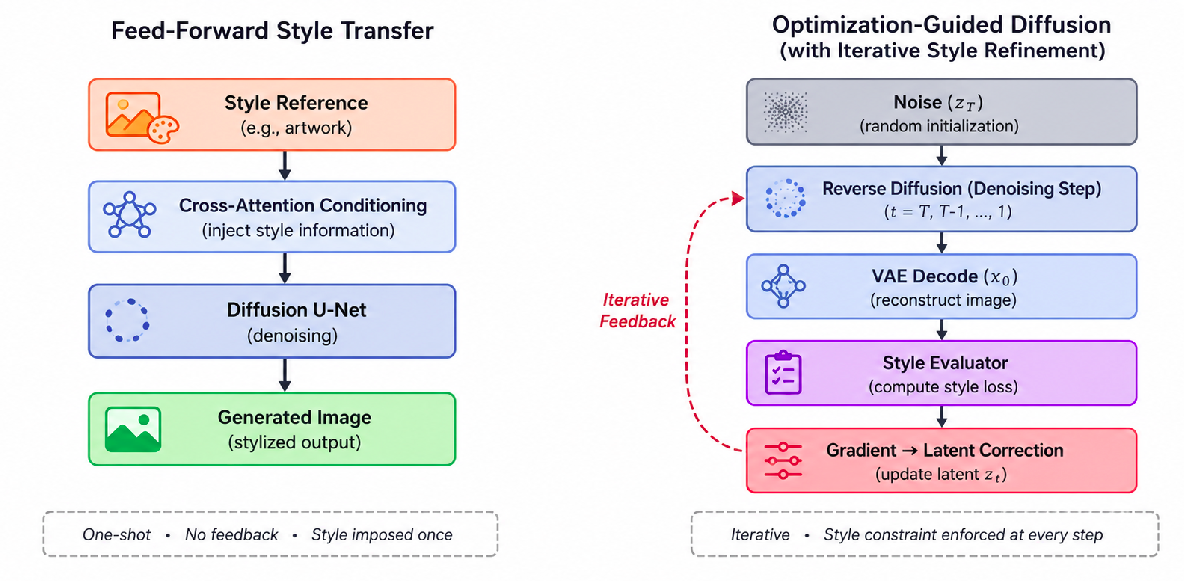
\includegraphics[width=0.95\linewidth]{images/figure_7.1.png}
    \caption{Conceptual comparison between the traditional feed-forward style transfer and the optimization-guided diffusion with iterative style refinement.}
    \label{fig:ch7_motivation}
\end{figure}

\FloatBarrier
% =====================================================
\section{Stable Diffusion with Constraints}
\label{sec:ch7_csd_theory}

Diffusion models have recently achieved remarkable success and become one of the most powerful frameworks for controllable image generation. Modern diffusion systems like Stable Diffusion~\cite{rombach2022ldm} and SDXL~\cite{podell2023sdxlimprovinglatentdiffusion} are able to produce very realistic images from text descriptions in an iterative denoising process over latent representations. While they have impressive capabilities, conventional diffusion models are inherently limited by the conditioning signals they have at inference. Once generation starts, the learned score function and the conditioning information provided mostly dictate the denoising trajectory, with little opportunity to impose external constraints.

Recent research has explored directly incorporating optimization objectives into the reverse diffusion process. These approaches, collectively known as constrained diffusion methods, aim to guide generated samples toward desired properties while preserving the generative capabilities of pretrained diffusion models. Diffusion is constrained by explicit objectives which are evaluated throughout the denoising process, not only via a prompt or reference image.

One of the most influential works in this direction is the constrained stable diffusion framework~\cite{zampini2025constrained}, which formulates image generation as a constrained optimisation problem. Instead of retraining model parameters, the framework operates fully at inference time by applying latent-space corrections defined by user-specified constraints. This formulation enables a pretrained diffusion model to meet external objectives without compromising generation quality or requiring extra supervision.

Let $z_t$ be the latent representation at diffusion timestep $t$. During normal diffusion sampling, the latent is evolved according to learned reverse diffusion dynamics. In the constrained setting, an additional objective function $g(x)$ is introduced, where
\begin{equation}
    x = D(z_t)
\end{equation}
denotes the decoded image from the frozen variational autoencoder (VAE) decoder $D(\cdot)$.

This constrained generation problem can be written as
\begin{equation}
    \min_x\; f(x) \quad \text{subject to} \quad g(x) \leq 0,
\end{equation}
where $f(x)$ is the diffusion objective and $g(x)$ is a user-specified constraint.

The main idea behind constrained diffusion is that generated samples can be periodically checked against the constraint function and corrected when violations occur. Instead of letting the denoising trajectory evolve naturally, optimization steps are introduced to guide latent representations to locations satisfying the desired constraints.

\begin{figure}[htbp]
    \centering
    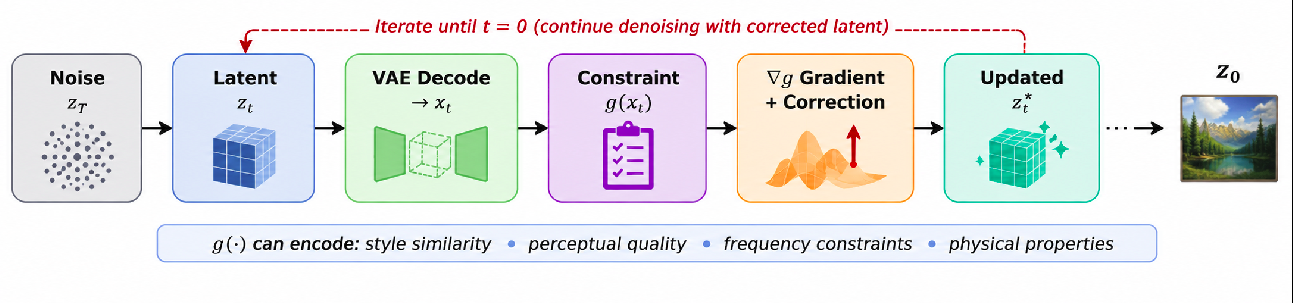
\includegraphics[width=0.95\linewidth]{images/figure_7.2.png}
    \caption{General constrained diffusion framework~\cite{zampini2025constrained}. Latent representations are decoded periodically, evaluated against a constraint function, and corrected before the denoising process continues.}
    \label{fig:ch7_csd_framework}
\end{figure}

One of the important advantages of this framework is flexibility. The constraint function can encode a wide class of objectives such as semantic similarity, style consistency, perceptual quality, physical properties, geometric constraints or task-specific requirements. Hence, constrained diffusion is a generic mechanism to inject external knowledge into image generation without modifying the pre-trained diffusion model itself.

An important benefit is the separation of generation and optimization. The constraint function guides the task, while the diffusion model is still responsible for generating realistic images. This modular design allows for the addition of new objectives without retraining the generative backbone and enables rapid experimentation with alternative constraint formulations.

Constrained diffusion provides an attractive alternative to traditional feed-forward conditioning in the setting of atmospheric style transfer. Instead of injecting style information solely via cross-attention mechanisms, atmospheric features can be modelled as optimisation objectives applied throughout the reverse diffusion process. This formulation enables continuous refinement of generated images and provides direct control over the evolution of atmospheric appearance during sampling.

\FloatBarrier
% =====================================================
\section{Style Guidance with Contrastive Style Descriptors}
\label{sec:ch7_csd_guidance}

The constrained diffusion framework outlined above provides a mechanism to incorporate arbitrary objectives into the reverse diffusion process. But the quality of the resulting guidance critically depends on the choice of constraint function. For atmospheric style transfer, an appropriate constraint is needed that captures visual properties associated with environmental phenomena but is robust to variations in scene content, object arrangement and semantic structure.

Existing style transfer approaches generally employ either low-level texture statistics or feature correlations obtained from convolutional neural networks. While such representations are suitable for artistic style transfer, they usually do not account for higher-level atmospheric properties like visibility degradation, color attenuation, illumination changes and the overall environmental appearance. Furthermore, these representations are often very sensitive to scene content, and thus not suitable for atmospheric style guidance where content preservation is desired.

To address these limitations, this work explores the use of Contrastive Style Descriptors (CSD)~\cite{somepalli2024csd} as a style-aware guidance mechanism. CSD is built on large-scale vision-language representations and is designed to separate style from semantic content. CSD learns a style representation that is consistent across different scenes with similar visual characteristics, unlike traditional feature extractors that mix object identity and appearance.

For a generated image $x_g$ and a reference style image $x_s$, the CSD encoder generates style embeddings as follows:
\begin{equation}
    s_g = S(x_g), \qquad s_s = S(x_s),
\end{equation}
where $S(\cdot)$ is the frozen style encoder.

The similarity between the generated style and the reference style is calculated by cosine similarity:
\begin{equation}
    \mathrm{Sim}(s_g, s_s) = \frac{s_g \cdot s_s}{\|s_g\|\,\|s_s\|}.
\end{equation}

A style loss can then be defined as:
\begin{equation}
    L_{\text{style}} = 1 - \mathrm{Sim}(s_g, s_s).
\end{equation}

Minimizing this objective encourages the generated images to be close to the target atmospheric style manifold while preserving the semantic information inherited from the diffusion model.

The proposed guidance mechanism is illustrated in Figure~\ref{fig:ch7_csd_guidance}. The latent representation is decoded into image space at selected diffusion timesteps, and passed through the frozen CSD encoder. The resulting style embedding is then compared to a reference atmospheric image and the resulting loss is backpropagated through the decoder to obtain gradients with respect to the latent representation. These gradients are then applied to improve the latent code before the denoising continues.

\begin{figure}[htbp]
    \centering
    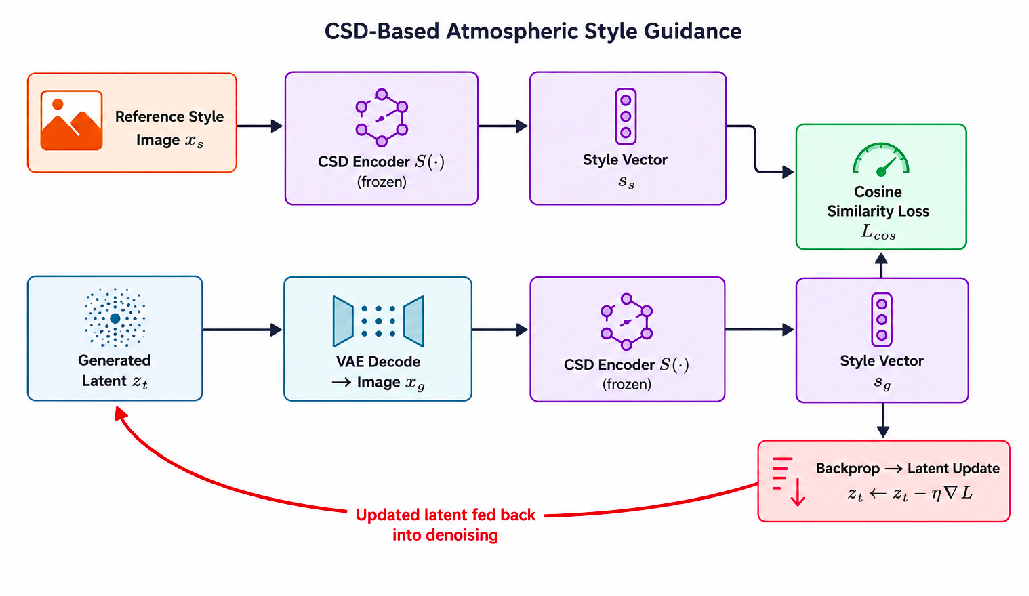
\includegraphics[width=0.95\linewidth]{images/figure_7.3.png}
    \caption{CSD-based atmospheric style guidance. Generated images are decoded from the latent representation, encoded by the frozen CSD network, and compared to a reference atmospheric style image.}
    \label{fig:ch7_csd_guidance}
\end{figure}

The main motivation for the use of CSD is the observation that the appearance statistics of atmospheric phenomena are often of a global nature rather than local texture patterns. Dense fog, haze, snowfall, underwater environments and sandstorms display distinct distributions of colour, contrast and visibility across the entire image. This means that the style embeddings learned with contrastive objectives are a better representation of atmospheric appearance than traditional texture-based descriptors.

The first hypothesis was that style similarity optimization in the CSD embedding space could enable direct control over the atmospheric look while maintaining content fidelity. If successful, the approach would provide a way of enforcing stylistic constraints over the reverse diffusion process, rather than relying only on feed-forward conditioning.

To test this hypothesis, a series of experiments was performed in which style losses based on CSD embeddings were included in the latent denoising process. The following section presents how these style objectives were propagated into the diffusion trajectory via gradient-based latent optimisation.

\begin{table}[htbp]
\centering
\caption{Initial CSD-guided diffusion configurations explored during atmospheric style transfer experiments.}
\label{tab:initial_csd}
\renewcommand{\arraystretch}{1.3}
\begin{tabular}{lll}
\toprule
\textbf{Experiment} & \textbf{Backbone} & \textbf{Guidance Objective} \\
\midrule
E1 & Stable Diffusion 1.5 & Cosine Similarity \\
E2 & Stable Diffusion 1.5 + LoRA & Cosine Similarity \\
E3 & SDXL & Cosine Similarity \\
E4 & SDXL & Cosine + Perceptual Loss \\
\bottomrule
\end{tabular}
\end{table}

\begin{figure}[htbp]
    \centering
    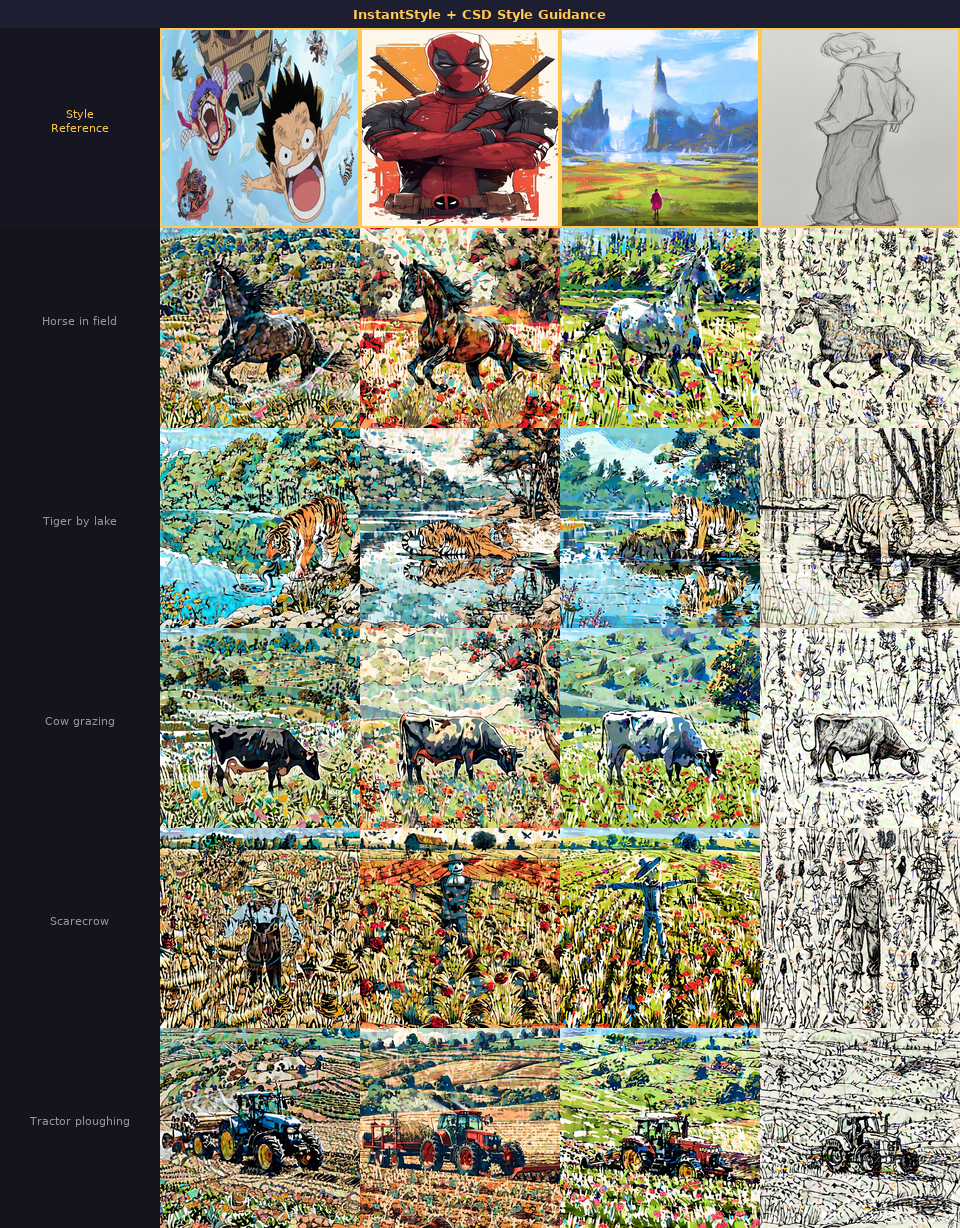
\includegraphics[width=0.88\linewidth, height=0.82\textheight, keepaspectratio]{images/ch7_grid_is_csd.png}
    \caption{InstantStyle + CSD guidance generation grid (seed 42). The first row shows the style reference image used as the guidance target for each atmospheric domain; subsequent rows show generated outputs for each content prompt. CSD guidance visibly shifts global appearance towards the target atmospheric domain, though aggressive gradient updates can introduce structural artefacts in complex scenes.}
    \label{fig:ch7_grid_is_csd}
\end{figure}

\FloatBarrier
% =====================================================
\section{Optimization in the Reverse Diffusion Process}
\label{sec:ch7_latent_opt}

The style constraint defined in the previous section provides a quantitative measure of the similarity between the atmospheric effect of a generated image and that of a reference style image. Having a suitable objective, however, is not sufficient on its own. To influence the generation process, the style loss must be backpropagated through the diffusion trajectory to modify the evolving latent representation.

Traditional diffusion sampling follows a fixed denoising path determined by the learned score function. At each time step, the model predicts a denoised prediction of the current latent representation, turning random noise step by step into a coherent image. In standard sampling, this process proceeds without any explicit feedback about whether the generated image is approaching the desired atmospheric style.

The main idea investigated in this work is to halt denoising at certain points in time and perform style-aware latent refinement. Instead of letting the latent representation evolve freely, the intermediate samples are decoded and evaluated through the CSD style encoder and corrected via gradient-based optimization.

Let $z_t$ be the latent representation at the diffusion step $t$. The latent is first decoded to image space using the frozen variational autoencoder:
\begin{equation}
    x_t = D(z_t),
\end{equation}
where $D(\cdot)$ denotes the VAE decoder.

The generated image is then fed into the CSD encoder to calculate the style loss:
\begin{equation}
    L_{\text{style}} = 1 - \cos\!\bigl(S(x_t),\; S(x_s)\bigr),
\end{equation}
where $x_s$ is the reference atmospheric style image.

Gradients are then calculated with respect to the latent representation:
\begin{equation}
    g_t = \nabla_{z_t} L_{\text{style}}.
\end{equation}

These gradients are used to perform a latent correction step:
\begin{equation}
    z_t' = z_t - \eta\, g_t,
\end{equation}
where $\eta$ is the learning rate for guidance.

The corrected latent representation is then fed back into the diffusion process and the denoising is continued normally until the next optimization step. This procedure is applied iteratively to steer the generated image toward the target atmospheric style manifold, while preserving the semantic structure inherited from the pretrained diffusion model.

\begin{figure}[htbp]
    \centering
    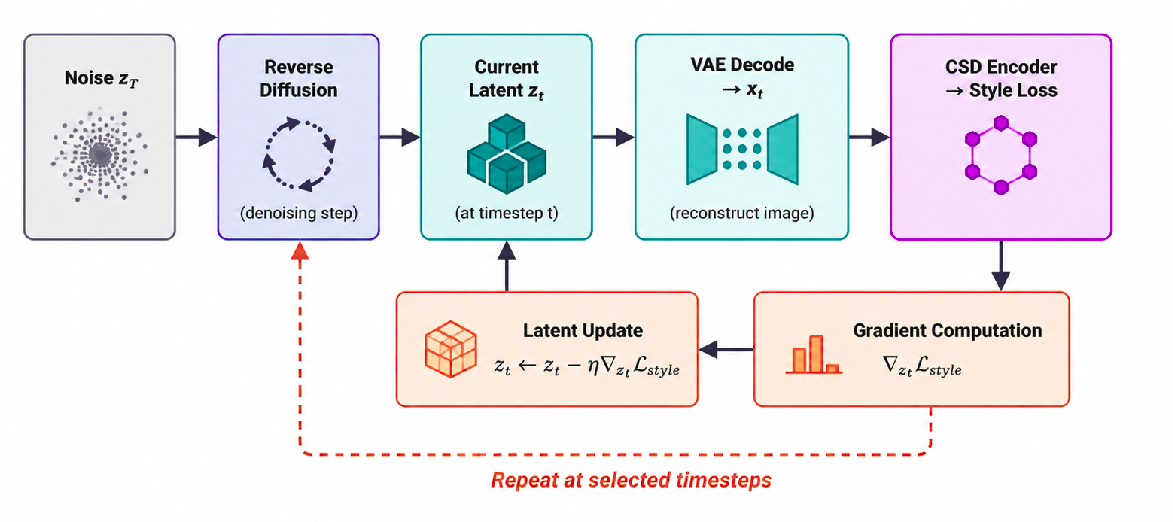
\includegraphics[width=0.95\linewidth]{images/figure_7.5.png}
    \caption{Optimization-guided refinement of latent representations. At selected timesteps the latent is decoded, evaluated by the style loss, corrected via gradient updates, and fed back into denoising.}
    \label{fig:ch7_latent_opt}
\end{figure}

One key design decision is the frequency of optimisation updates. Correcting at each denoising step adds large computational overhead and can destabilise the diffusion trajectory. Infrequent updates, however, may provide insufficient guidance to steer the final image. A range of update schedules was investigated, from dense optimisation throughout the full denoising process to sparse corrections applied only at later generation stages.

Another important factor is the scale of the guidance signal. Excessively large latent corrections can overpower the diffusion prior, leading to unrealistic images, semantic distortions, or collapse toward the reference style image. Very small updates, conversely, do not produce meaningful atmospheric transformations. Balancing generation fidelity and style adherence therefore emerged as one of the central challenges of optimisation-guided diffusion.

Initial experiments confirmed that simple latent correction can influence global image appearance and improve similarity with the target style distribution. The behaviour obtained, however, depends strongly on the choice of optimisation hyperparameters, guidance schedules, and diffusion backbone. Aggressive optimisation frequently produced unrealistic visual results or destroyed important semantic information present in the original scene.

These observations motivated further investigation into the relationship between guidance strength and content preservation. Experiments with different optimisation schedules showed that the timing of style corrections is critical for output quality. The following section examines this relationship via Langevin dynamics and stochastic latent refinement.

\begin{table}[htbp]
\centering
\caption{Optimization parameters explored during latent refinement experiments.}
\label{tab:latent_optimization}
\renewcommand{\arraystretch}{1.3}
\begin{tabular}{lll}
\toprule
\textbf{Parameter} & \textbf{Values Tested} & \textbf{Reason} \\
\midrule
Learning rate & 0.001 -- 0.1 & Control update magnitude \\
Guidance Frequency & Sparse / Dense & Update scheduling \\
Optimization Steps & 1 -- 10 & Correction strength \\
Diffusion Backbone & SD1.5 / SDXL & Model comparison \\
Style Objective & Cosine Similarity & Atmospheric alignment \\
\bottomrule
\end{tabular}
\end{table}

\FloatBarrier
% =====================================================
\section{Langevin Dynamics for Latent Refinement}
\label{sec:ch7_langevin}

The previous section describes a gradient-based optimization strategy that showed that the atmospheric style characteristics can be manipulated with a latent correction strategy. However, the updates generated were entirely deterministic and frequently behaved unstably. In several experiments, strong style gradients caused a significant deviation of the optimization process from the natural diffusion trajectory, leading to distorted structures, unrealistic textures and severe semantic degradation.

This observation led us to explore stochastic optimization techniques that can balance style guidance with the inherent generative prior of the diffusion model. Among the approaches available, Langevin Dynamics is especially attractive, as it combines gradient-based optimization with controlled stochastic exploration.

Langevin Dynamics is a technique developed for Bayesian inference and sampling from complex probability distributions. It adds Gaussian noise to the deterministic gradient updates. This additional stochastic term allows samples to explore nearby regions of the latent space while still moving towards regions that satisfy the desired objective.

The Langevin update for a latent representation $z_t$ can be written as:
\begin{equation}
    z_{t+1} = z_t - \eta\,\nabla_z L(z_t) + \sqrt{2\eta}\,\epsilon_t,
\end{equation}
where $\eta$ is the optimization step size, $L(z_t)$ is the style objective, and $\epsilon_t \sim \mathcal{N}(0, I)$ is Gaussian noise.

The extra stochastic term serves two important purposes over the deterministic latent correction strategy introduced above. First, it keeps optimization from getting stuck in bad local minima. Second, it maintains sample diversity by ensuring that the latent trajectories keep exploring reasonable regions of the diffusion manifold.

\begin{figure}[htbp]
    \centering
    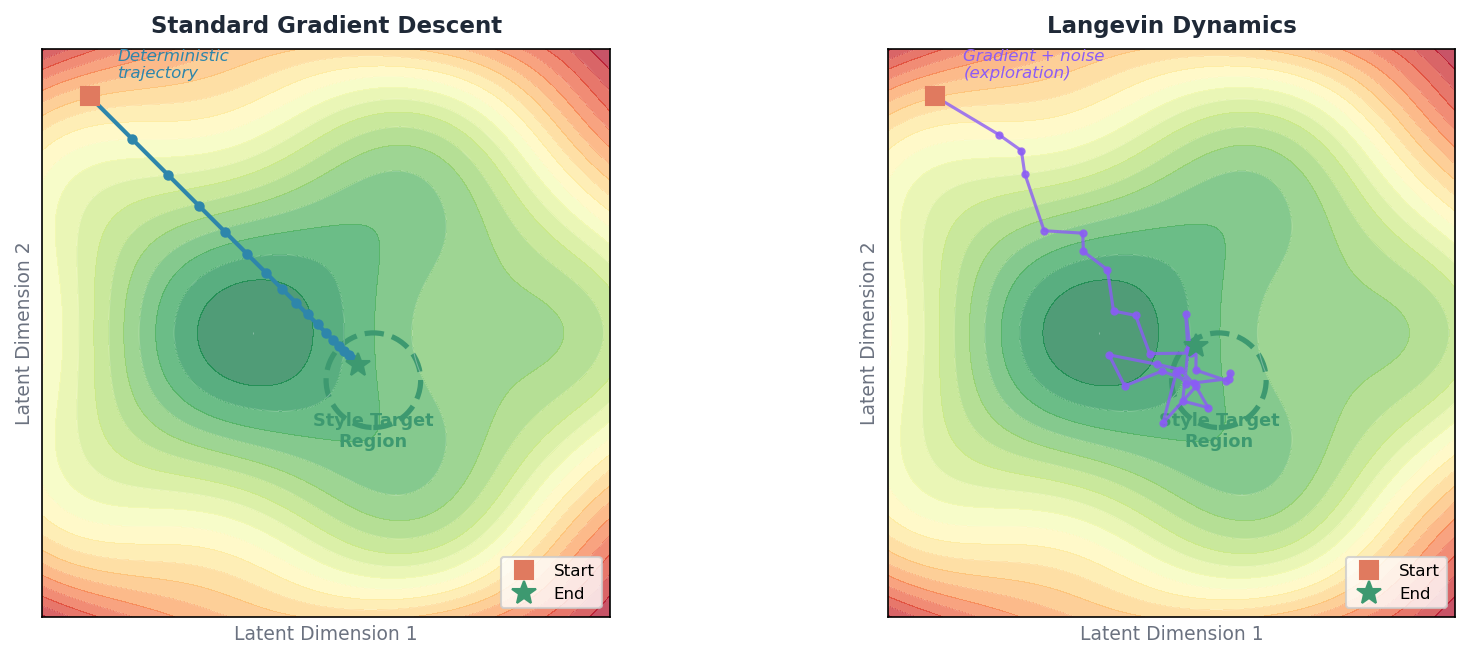
\includegraphics[width=0.95\linewidth]{images/ch7_langevin_concept.png}
    \caption{Conceptual depiction of the Langevin-based latent refinement. The latent representation is optimized toward high style similarity while preserving stochastic exploration of the diffusion manifold.}
    \label{fig:ch7_langevin_concept}
\end{figure}

A set of experiments was performed, using Langevin refinement at different stages of the denoising process. In the first experiments the optimization updates were applied along the entire reverse diffusion trajectory. While this approach resulted in higher style similarity scores, the generated images often suffered from severe semantic distortions. Foreground objects were partially corrupted, structural details were lost and in extreme cases the generated image began to look more like the reference style image than the original content.

Representative failure cases encountered in early experiments are illustrated in Figure~\ref{fig:ch7_langevin_failure}. Strong optimization caused the latent representation to deviate from the natural diffusion path, resulting in unnatural image formation and reduced content preservation.

\begin{figure}[htbp]
    \centering
    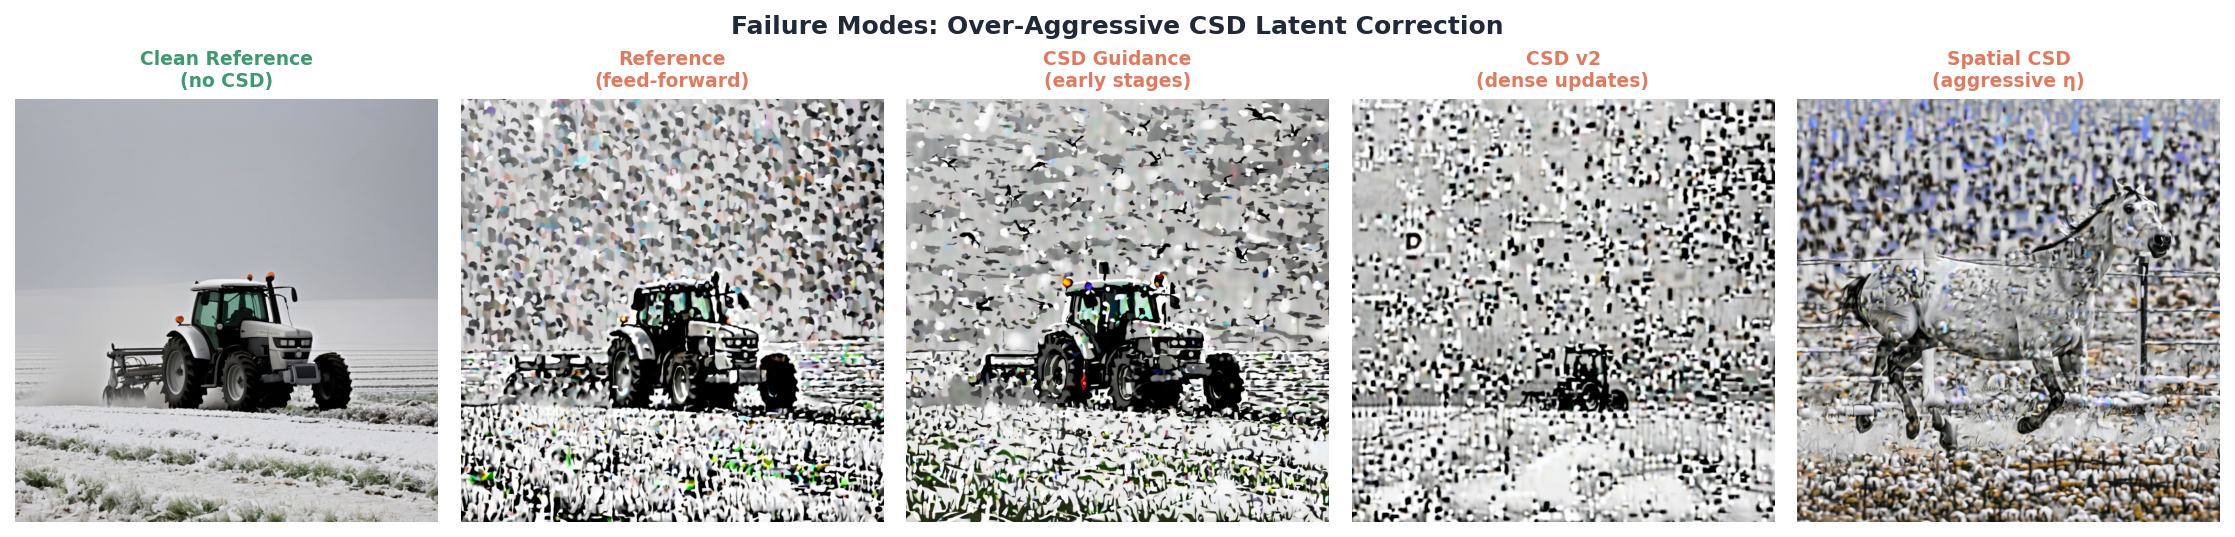
\includegraphics[width=0.95\linewidth]{images/ch7_langevin_failure.png}
    \caption{Typical failure cases observed in early Langevin-guided experiments. The aggressive optimization led to semantic collapse, structural distortions, and large-scale style leakage from the reference image.}
    \label{fig:ch7_langevin_failure}
\end{figure}

Further analysis showed that the performance of Langevin guidance is highly dependent on the stage in the diffusion process at which the optimization is applied. The overall semantic layout of the generated image is mostly decided by the early denoise steps. Therefore, strong style guidance at these stages often disrupts object formation and scene layout. In contrast, later denoising steps focus on refining appearance-level details and are thus a more suitable stage for optimizing atmospheric style.

In order to investigate this phenomenon, several optimization schedules were studied. The schedules differed in when they started the Langevin updates and how often they corrected during generation. Results consistently showed that the late-stage guidance led to better content preservation, while still making meaningful changes to the atmosphere.

Another important observation was the sensitivity of the optimization process to the selection of the learning rate. Small learning rates produced little stylistic change, while too large values destabilized generation and increased the chance of semantic collapse. It was found that a narrow intermediate range provided the best compromise between atmospheric realism and preservation of structure.

The main hyperparameters investigated in Langevin-guided diffusion experiments are summarized in Table~\ref{tab:langevin_hyperparameters}.

\begin{table}[htbp]
\centering
\caption{Hyperparameter configurations explored in Langevin-guided diffusion experiments.}
\label{tab:langevin_hyperparameters}
\renewcommand{\arraystretch}{1.3}
\begin{tabular}{lll}
\toprule
\textbf{Parameter} & \textbf{Values Explored} & \textbf{Observation} \\
\midrule
Learning rate & 0.001 -- 0.1 & Strength of style controlling \\
Optimization frequency & Sparse / Dense & Stability influence \\
Guidance Start Step & Early / Mid / Late & Impacts content preservation \\
Optimization Iterations & 1 -- 10 & Controls convergence \\
Noise Strength & Variable & Balances exploration \\
\bottomrule
\end{tabular}
\end{table}

Experiments also showed the limitations of unconstrained stochastic optimization, though Langevin refinement improved controllability over simple latent correction. The generated images were often inconsistent in their goals and it was still hard to find a stable trade-off between atmospheric style and semantic structure. These observations motivated the search for more principled optimization frameworks that can explicitly enforce constraints while preserving fidelity to the original diffusion trajectory.

We now consider Proximal Langevin Dynamics, which employs projection-based updates that constrain the latent corrections to feasible regions of the solution space. This formulation leads to a more stable mechanism for incorporating style constraints and ultimately forms the basis for the final optimization-driven framework investigated in this chapter.

\FloatBarrier
% =====================================================
\section{Proximal Langevin Dynamics}
\label{sec:ch7_pld}

The preceding section demonstrated that stochastic latent refinement can improve the atmospheric style match during diffusion sampling. However, unconstrained Langevin updates frequently introduced instability into the generation process. Strong optimization steps tended to cause latent trajectories to diverge from the natural diffusion manifold, resulting in semantic collapse, structural artifacts and over-reliance on the reference style image.

These observations illustrate a fundamental difficulty in optimization-guided diffusion. Stricter guidance generally leads to better style adherence at the cost of degrading image realism and content preservation. Therefore, a successful optimization framework needs to balance two conflicting objectives: preserving the fidelity to the learned diffusion prior, and satisfying the desired style constraints.

To overcome this limitation, the investigation turned to Proximal Langevin Dynamics (PLD), a constrained optimization framework that incorporates stochastic exploration and projection-based correction. Unlike the traditional Langevin update that directly updates the latent representations using the gradient information, PLD introduces an additional projection step to restrict the updates to a feasible region of the solution space.

The general proximal Langevin update can be written as:
\begin{equation}
    x_{t+1} = \mathrm{prox}_{\lambda g}\!\left( x_t + \gamma_t\,\nabla\log p(x_t) + \sqrt{2\gamma_t}\,\epsilon_t \right),
    \label{eq:proximal_loop}
\end{equation}
where $x_t$ is the current sample, $\gamma_t$ is the step size, $\epsilon_t$ is Gaussian noise, $g(\cdot)$ is the constraint function, and $\mathrm{prox}_{\lambda g}$ is the proximal operator.

The proximal operator acts as a projection mechanism that prevents the optimization from straying too far from areas that satisfy the desired constraints. PLD always maintains a balance between the diffusion objective and the constraint objective rather than allowing free latent updates. This results in a more stable optimization process.

\begin{figure}[htbp]
    \centering
    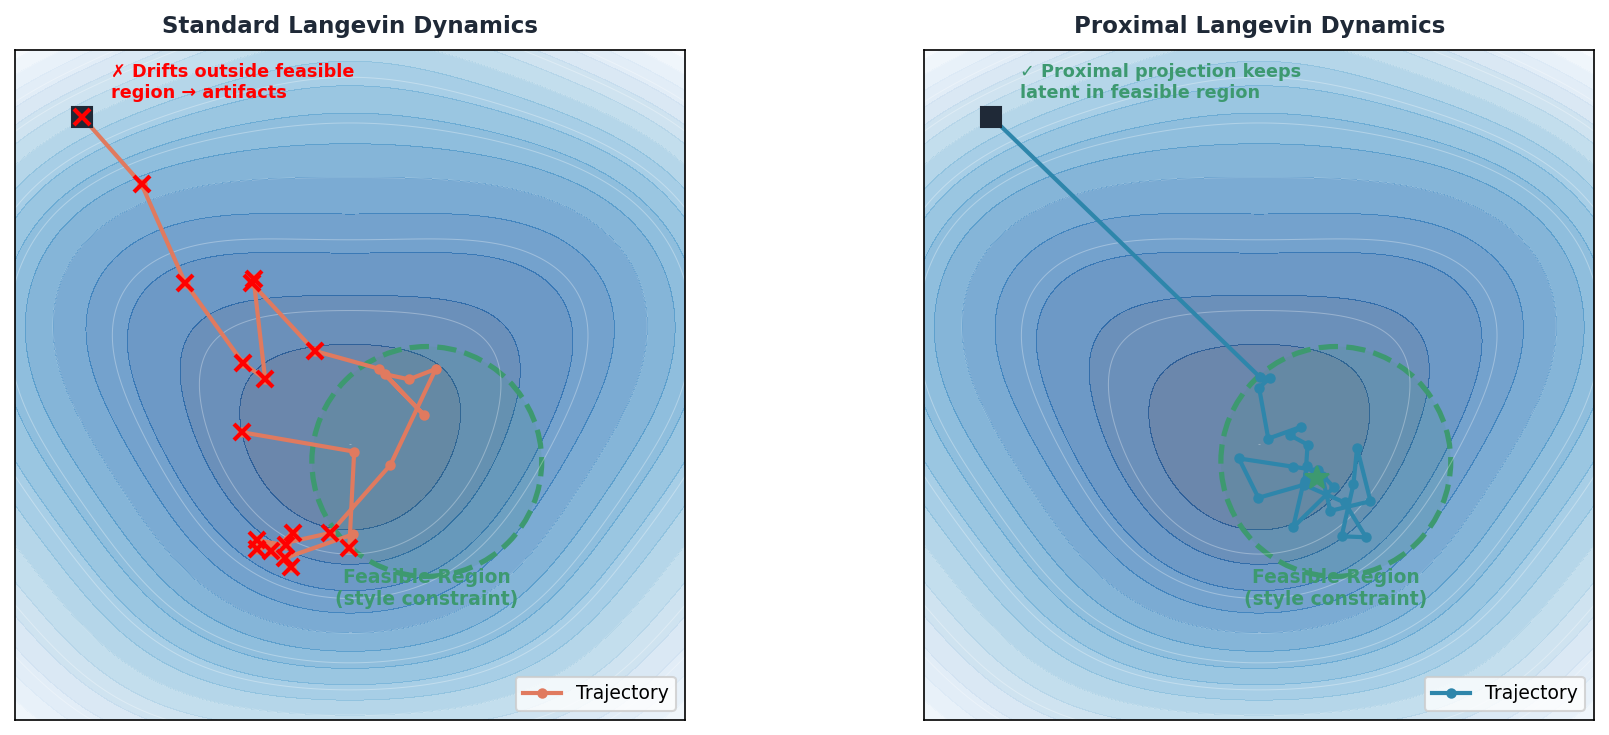
\includegraphics[width=0.95\linewidth]{images/ch7_pld_comparison.png}
    \caption{Unconstrained Langevin updates vs.\ Proximal Langevin Dynamics. The proximal operator restricts latent updates, preventing divergence from the diffusion manifold while enforcing the style constraint.}
    \label{fig:ch7_pld_comparison}
\end{figure}

In atmospheric style transfer, the proximal constraint was derived from style similarity objectives computed using CSD embeddings. The resulting image was decoded at selected time steps and compared to a reference image of atmospheric style. The calculated style loss was used to define a feasible region corresponding to acceptable atmospheric similarity.

This formulation has several advantages over standard latent correction. First, it reduces sensitivity to learning rate selection by bounding the magnitude of individual updates. Second, it reduces semantic collapse by avoiding large deviations from the prior diffusion. Third, it offers a principled way to incorporate multiple constraint functions into a unified optimization framework.

We could also include more sophisticated guidance objectives thanks to the use of proximal operators. Besides a simple cosine similarity, one could incorporate perceptual losses, feature-space statistics and frequency-domain constraints into the optimization procedure and still keep the generation behaviour stable.

Another advantage of PLD is that it is compatible with adaptive guidance schedules. The proximal formulation allows the strength of the guidance to adapt to the current denoising step, instead of a fixed optimization strength during the generation. This capability was found to be particularly useful for atmospheric style transfer, where different stages of the diffusion process play different roles in semantic structure and appearance formation.

The experimental results revealed that proximal Langevin updates consistently produced more stable results compared to standard Langevin refinement. The images exhibited better content preservation, less structural distortions, and smoother transitions to the target atmospheric style distribution. Although optimization was still computationally expensive, the increased stability of PLD made it the most promising optimization framework considered in this phase of the investigation.

The addition of proximal constraints also allowed us to explore richer style representations than the standard cosine similarity objectives. In particular, the atmospheric effects of fog, haze, snow and underwater images have specific frequency-domain properties that are not fully represented solely by embedding-space similarity. The next section therefore investigates how perceptual and frequency-aware constraints may be integrated into the optimization framework.

\begin{table}[htbp]
\centering
\caption{Comparison of latent correction, Langevin dynamics and proximal Langevin dynamics.}
\label{tab:optimization_comparison}
\renewcommand{\arraystretch}{1.3}
\begin{tabular}{lccc}
\toprule
\textbf{Method} & \textbf{Stability} & \textbf{Style Control} & \textbf{Content Preservation} \\
\midrule
Latent Correction & Medium & Medium & Medium \\
Langevin Dynamics & Low & High & Low \\
Proximal Langevin Dynamics & High & High & High \\
\bottomrule
\end{tabular}
\end{table}

\begin{figure}[htbp]
    \centering
    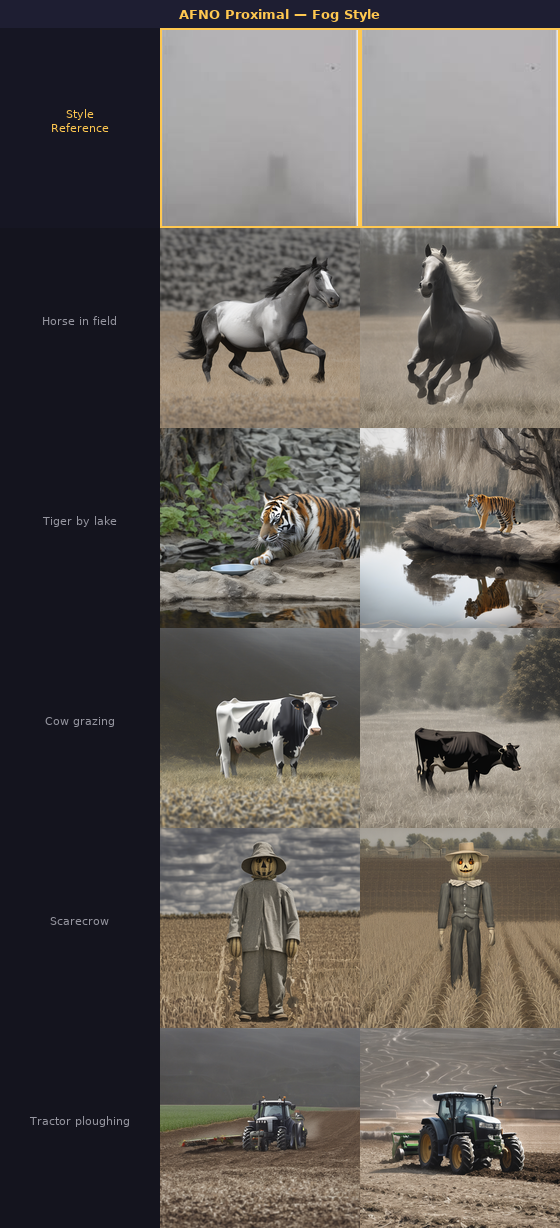
\includegraphics[width=0.6\linewidth, height=0.72\textheight, keepaspectratio]{images/ch7_grid_afno_proximal.png}
    \caption{Fog style transfer results using AFNO-based Proximal Langevin Dynamics (seed 42 and 123). The first row shows the fog style reference used as the optimisation target; subsequent rows show generated outputs per content prompt. The proximal projection operator constrains each latent update to the feasible region, yielding stable atmospheric transformations while preserving structural coherence.}
    \label{fig:ch7_afno_proximal}
\end{figure}

\FloatBarrier
% =====================================================
\section{Frequency-Based and Perceptual Constraints}
\label{sec:ch7_frequency}

The optimisation frameworks described in the previous sections are mostly based on style similarity computed in the CSD embedding space. These representations gave a semantically meaningful description of visual appearance, but empirical observations indicated that embedding similarity alone could not reliably capture atmospheric features.

Although the atmospheric behaviour was unrealistic, several generated images obtained high style similarity scores. In many cases the generated images were close to the reference style image in terms of overall colour distribution, but important atmospheric properties such as visibility degradation, contrast attenuation and depth-dependent scattering were still not well represented. These findings indicated that the semantic style embeddings fail to completely describe the atmospheric appearance.

Atmospheric phenomena are driven by physical image formation and global image statistics. Dense fog attenuates high-frequency image content, haze attenuates contrast as a function of depth, snowfall introduces structured texture patterns, and underwater environments generate wavelength-dependent colour attenuation. Thus, a guidance signal that relies solely on embedding similarity might fail to capture critical atmospheric features.

To address this limitation, the optimisation framework was augmented with additional perceptual and frequency-domain objectives. These objectives provide complementary information that is not explicitly available in the CSD embedding space, thereby offering a more complete description of atmospheric appearance.

\subsection{Perceptual Constraints}
\label{sec:ch7_perceptual}

Perceptual losses have become very popular in the areas of image synthesis and style transfer, since they compare images in a learned feature space instead of pixel-wise differences. Perceptual objectives operate on intermediate representations extracted from deep neural networks instead of directly measuring similarity in the image space.

Given a set of feature activations extracted from a pretrained encoder, the perceptual similarity can be expressed as:
\begin{equation}
    L_{\text{perc}} = \sum_{l} \bigl\|\phi_l(x_g) - \phi_l(x_s)\bigr\|_2^2,
\end{equation}
where $\phi_l(\cdot)$ is the activation of layer $l$, $x_g$ is the generated image and $x_s$ is the reference style image.

The main motivation for introducing perceptual guidance is the observation that atmospheric effects affect the structure of the image at a variety of scales. Local texture statistics, object boundaries, and global contrast relations all contribute to the perception of the environmental conditions. Such characteristics are captured by perceptual feature spaces, which therefore provide a richer representation of the atmospheric appearance than embedding similarity alone.

Experimental results showed that perceptual constraints improved content preservation and reduced a number of failure modes observed during cosine-only guidance. The generated images had more realistic atmospheric transitions and better preserved the structure of objects.

\subsection{Frequency-Domain Constraints}
\label{sec:ch7_freq}

Although perceptual guidance improved structural consistency, atmospheric phenomena have unique frequency-domain signatures not explicitly represented by feature-space objectives.

Fog, haze, smoke and underwater imagery are all associated with the attenuation of the high frequency image components. Increasing the atmospheric density suppresses fine details more and more, while the low frequency structures are relatively unaffected. Such behaviour can be seen directly in the Fourier spectrum of atmospheric images.

This observation motivated introducing constraints in the frequency domain through the Fourier Transform. The frequency representation of a generated image $x_g$ is calculated as:
\begin{equation}
    F_g = \mathcal{F}(x_g),
\end{equation}
where $\mathcal{F}(\cdot)$ is the two-dimensional Fourier Transform. The reference style image is represented as:
\begin{equation}
    F_s = \mathcal{F}(x_s).
\end{equation}

A frequency consistency objective can then be formulated as:
\begin{equation}
    L_{\text{freq}} = \bigl\| |F_g| - |F_s| \bigr\|_2^2,
\end{equation}
where $|F|$ is the magnitude spectrum.

The frequency loss promotes the generated images to share similar spectral characteristics of the target atmospheric domain. Unlike embedding-based objectives, this formulation imposes direct constraints on the distribution of image frequencies, providing a more physically meaningful description of visibility degradation.

\begin{figure}[htbp]
    \centering
    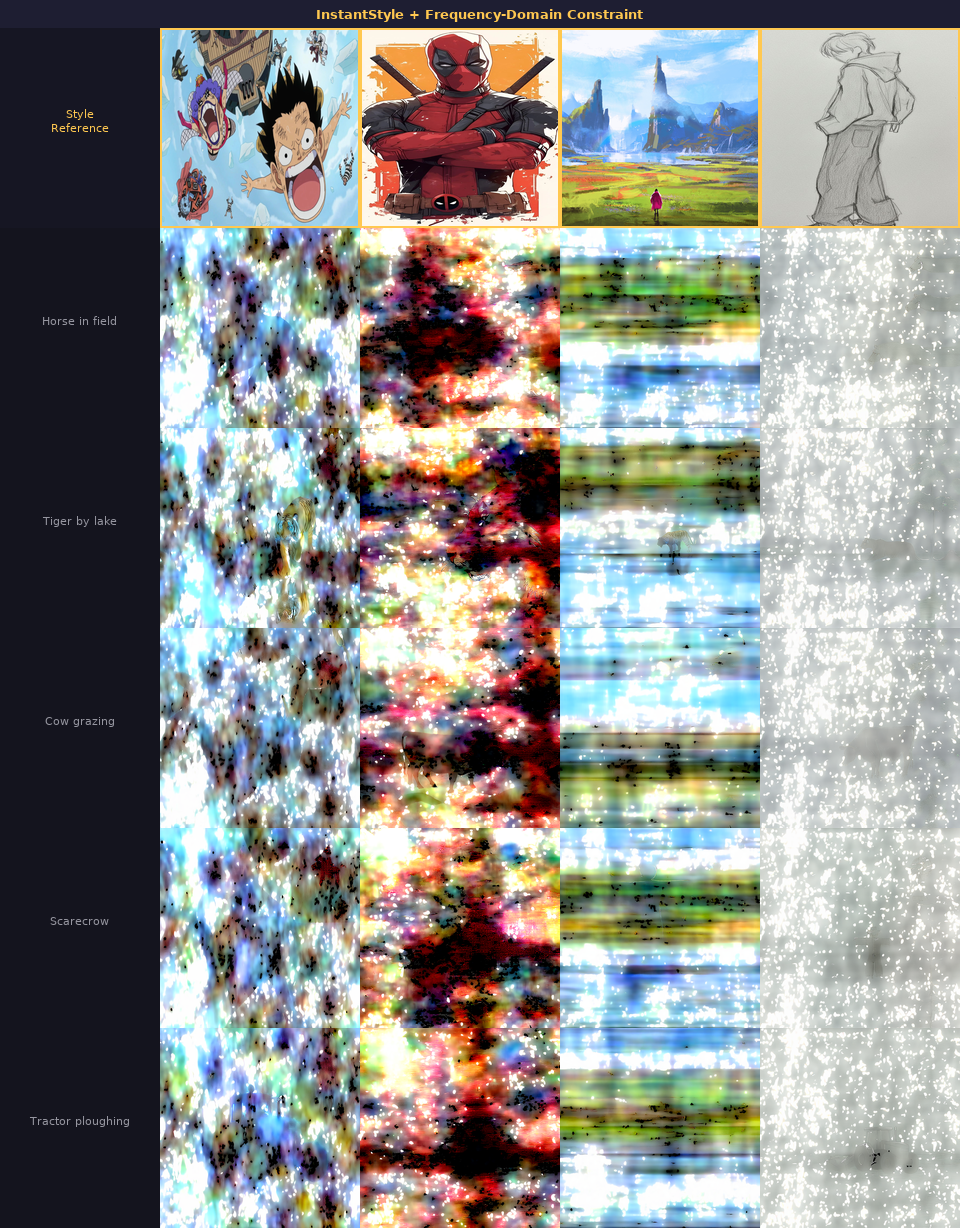
\includegraphics[width=0.88\linewidth, height=0.82\textheight, keepaspectratio]{images/ch7_grid_is_freq.png}
    \caption{InstantStyle + Frequency-domain constraint generation grid (seed 42). The first row shows the style reference image for each atmospheric domain; subsequent rows show generated outputs per content prompt. The FFT magnitude loss encourages the spectral envelope of each generated image to match the reference, producing more pronounced high-frequency attenuation characteristic of fog and sandstorm conditions.}
    \label{fig:ch7_grid_is_freq}
\end{figure}

\begin{figure}[htbp]
    \centering
    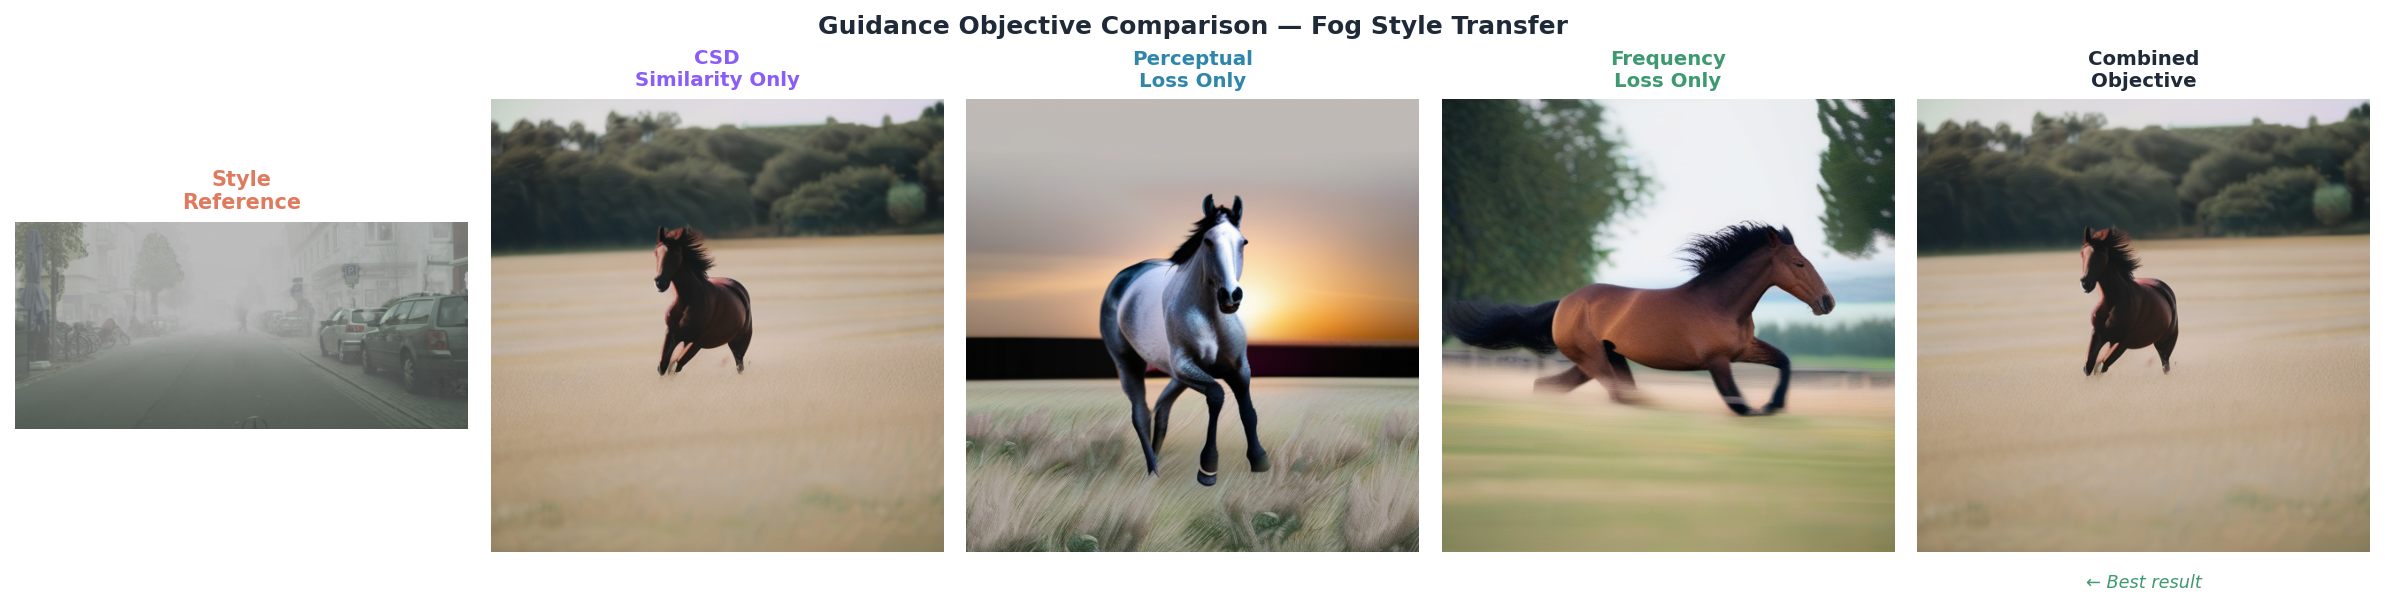
\includegraphics[width=0.95\linewidth]{images/ch7_objective_comparison.png}
    \caption{Comparison of different guidance objectives for atmospheric style transfer. The combined objective produces the most visually convincing results.}
    \label{fig:ch7_objective_comparison}
\end{figure}

\subsection{Combined Objective}
\label{sec:ch7_combined}

The final optimization framework consisted of multiple complementary objectives to capture different aspects of atmospheric appearance. The overall guidance objective is formulated as:
\begin{equation}
    L_{\text{total}} = \lambda_s\,L_{\text{style}} + \lambda_p\,L_{\text{perc}} + \lambda_f\,L_{\text{freq}},
\end{equation}
where $L_{\text{style}}$ is the CSD similarity loss, $L_{\text{perc}}$ is the perceptual guidance, and $L_{\text{freq}}$ is the frequency-domain consistency. The relative importance of each component is controlled by the weighting coefficients $\lambda_s$, $\lambda_p$ and $\lambda_f$.

Empirical evaluation showed that the joint objective always outperformed any individual loss term in producing more convincing atmospheric transformations. The style similarity guaranteed the semantic consistency with the reference image, the perceptual guidance preserved the structure of the scene, and the frequency constraints guided the realistic atmospheric degradation patterns. These objectives together provided a much richer representation of the atmospheric appearance, and laid the foundation for the final optimization-driven diffusion framework explored in this chapter.

\begin{table}[htbp]
\centering
\caption{Qualitative comparison of optimization objectives used in atmospheric style guidance experiments.}
\label{tab:objective_comparison}
\renewcommand{\arraystretch}{1.3}
\begin{tabular}{lccc}
\toprule
\textbf{Objective} & \textbf{Style Fidelity} & \textbf{Content Preservation} & \textbf{Stability} \\
\midrule
CSD Similarity & Medium & High & Medium \\
Perceptual Loss & Medium & High & High \\
Frequency Loss & High & Medium & Medium \\
Combined Objective & High & High & High \\
\bottomrule
\end{tabular}
\end{table}

\FloatBarrier
% =====================================================
\section{Experimental Progress and Discussion}
\label{sec:ch7_experiments}

The experiments described in this chapter were performed at different points in the development, each stage being prompted by observations from previous iterations. Instead of being developed from a fully optimization-guided framework from the start, the study was developed step-by-step through a series of experiments that aimed to understand the interaction between style constraints and diffusion-based image generation.

\subsection{Baseline Experiments: IP-Adapter on SDXL}
\label{sec:ch7_sd15}

Early experiments began with Stable Diffusion 1.5~\cite{rombach2022ldm}, confirming that direct CSD latent correction on the smaller backbone produced weak atmospheric effects and was highly sensitive to the learning rate. These results motivated a move to SDXL~\cite{podell2023sdxlimprovinglatentdiffusion}, whose richer latent representations and stronger generative prior offered a more stable foundation for optimization-based guidance.

The first SDXL experiments used IP-Adapter~\cite{ye2023ipadapter} as a feed-forward style conditioning baseline — no optimization guidance, just the adapter injecting style tokens into the cross-attention layers. Figure~\ref{fig:ch7_grid_ipadapter} shows the full generation grid across all tested style domains and content prompts. While the adapter transfers artistic styles (anime, comic, digital painting) convincingly, the atmospheric fog column is notably weak: generated images remain visually close to a clear-day scene, with no meaningful visibility degradation or haze formation. This confirms that feed-forward conditioning alone is insufficient for atmospheric style transfer and motivates the optimization-guided approaches explored throughout this chapter.

\begin{figure}[htbp]
    \centering
    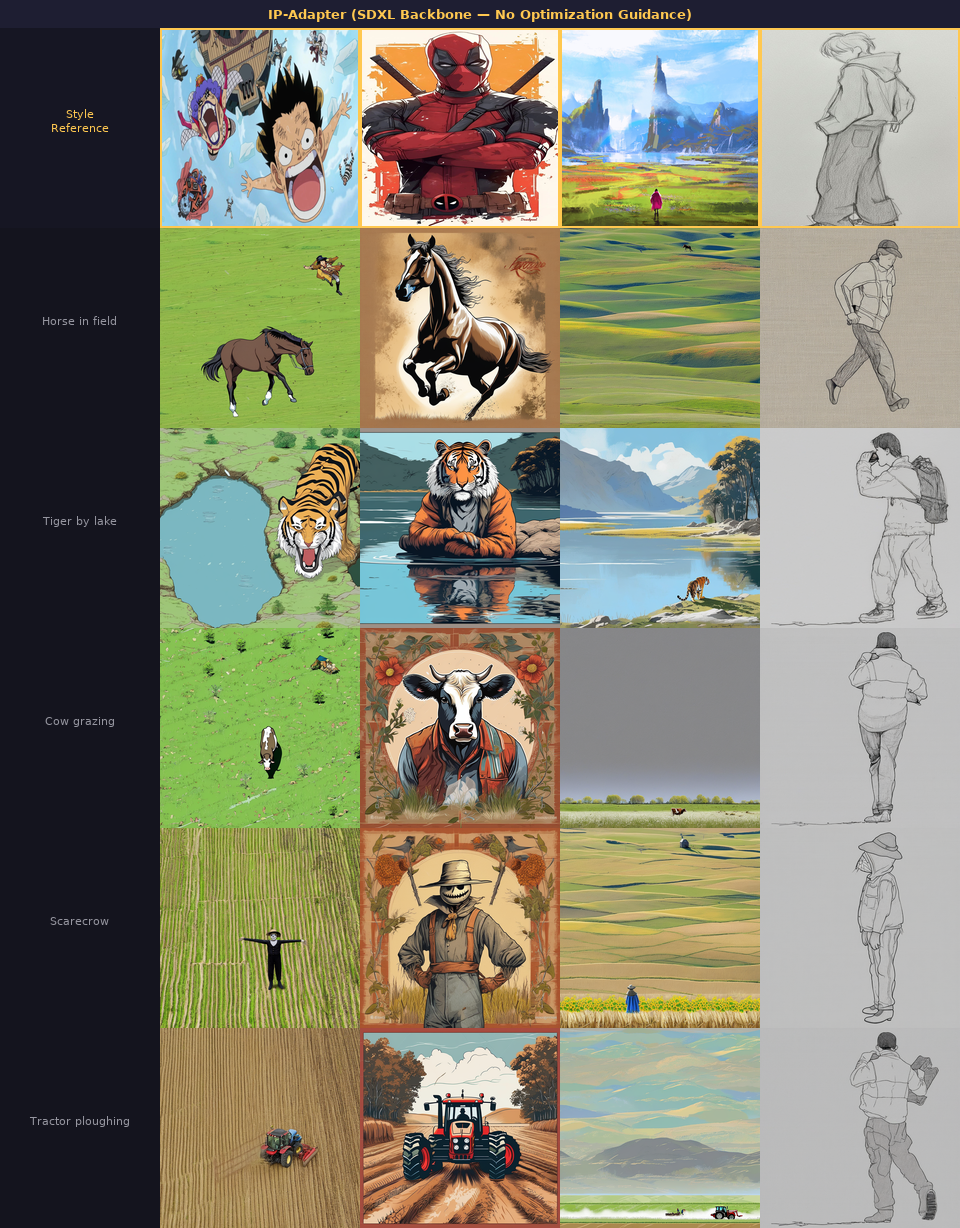
\includegraphics[width=0.95\linewidth]{images/ch7_grid_ipadapter.png}
    \caption{IP-Adapter (SDXL backbone) generation grid — seed 42. The first row in each style column shows the style reference image. Artistic styles (anime, comic, digital painting) transfer well; the fog\_style column produces clear-day images with negligible atmospheric effect, illustrating the limitation of feed-forward conditioning for atmospheric style transfer.}
    \label{fig:ch7_grid_ipadapter}
\end{figure}

\FloatBarrier
\subsection{Naive CSD Guidance and Its Failure Modes}
\label{sec:ch7_lora}

The natural next step was to augment IP-Adapter with CSD latent correction, applying gradient-based updates from the style loss throughout the denoising process. The expectation was that the optimization signal would bridge the gap the adapter could not close. In practice the opposite occurred: unconstrained CSD latent correction completely destabilised generation.

Figure~\ref{fig:ch7_grid_fog_failure} isolates the fog style domain to make the failure unambiguous: the IP-Adapter baseline (centre column) achieves plausible foggy scenes, confirming that the backbone and style injection work correctly. Adding unconstrained CSD latent correction (right column) collapses every single output into incoherent noise — the gradient signal overwhelms the diffusion prior and erases all semantic content. Figure~\ref{fig:ch7_grid_ipadapter_csd} shows that this collapse is not fog-specific; it occurs uniformly across all style domains and all content prompts. These failure modes reveal the core tension explored in the rest of this chapter: the style gradient must be introduced carefully, otherwise it destroys the very image structure it is meant to modify.

\begin{figure}[H]
    \centering
    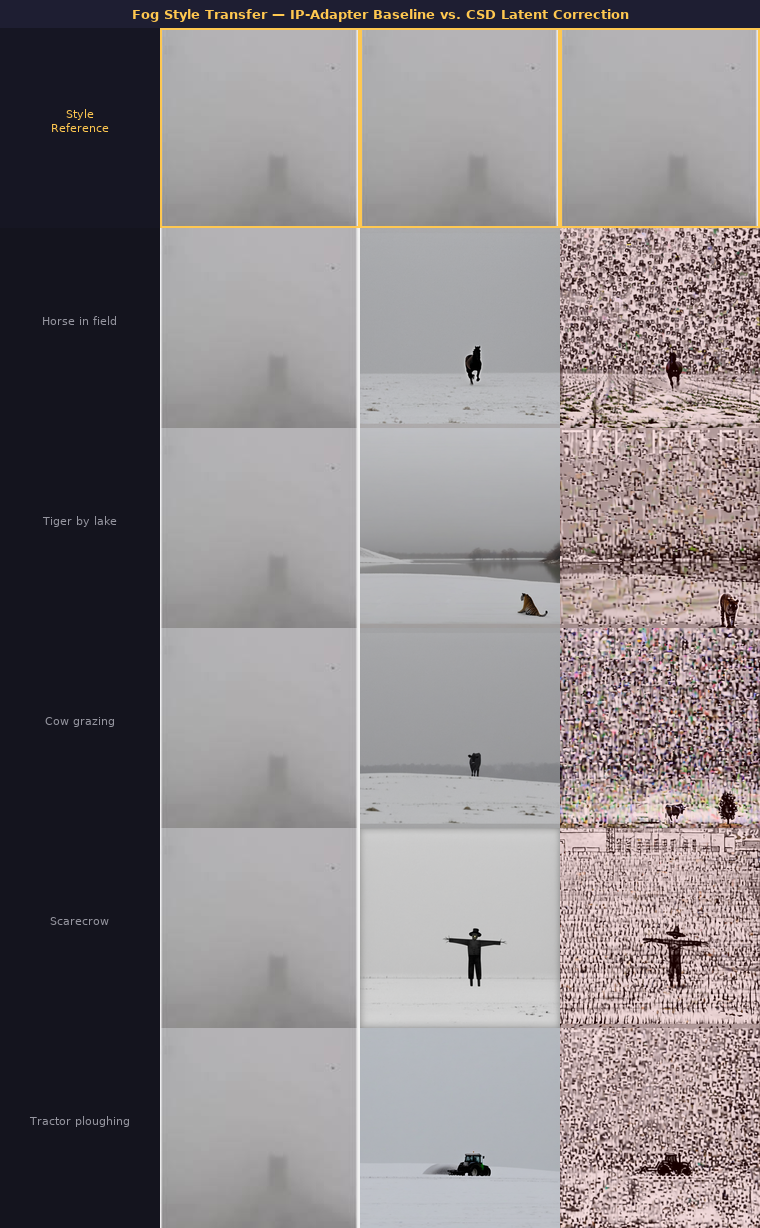
\includegraphics[width=0.44\linewidth]{images/ch7_grid_fog_failure.png}
    \caption{Fog-domain comparison (seed 42). \textbf{Centre column:} IP-Adapter alone produces plausible foggy scenes. \textbf{Right column (red tint):} adding unconstrained CSD latent correction destroys the image entirely, leaving tiled noise artefacts.}
    \label{fig:ch7_grid_fog_failure}
\end{figure}

\begin{figure}[htbp]
    \centering
    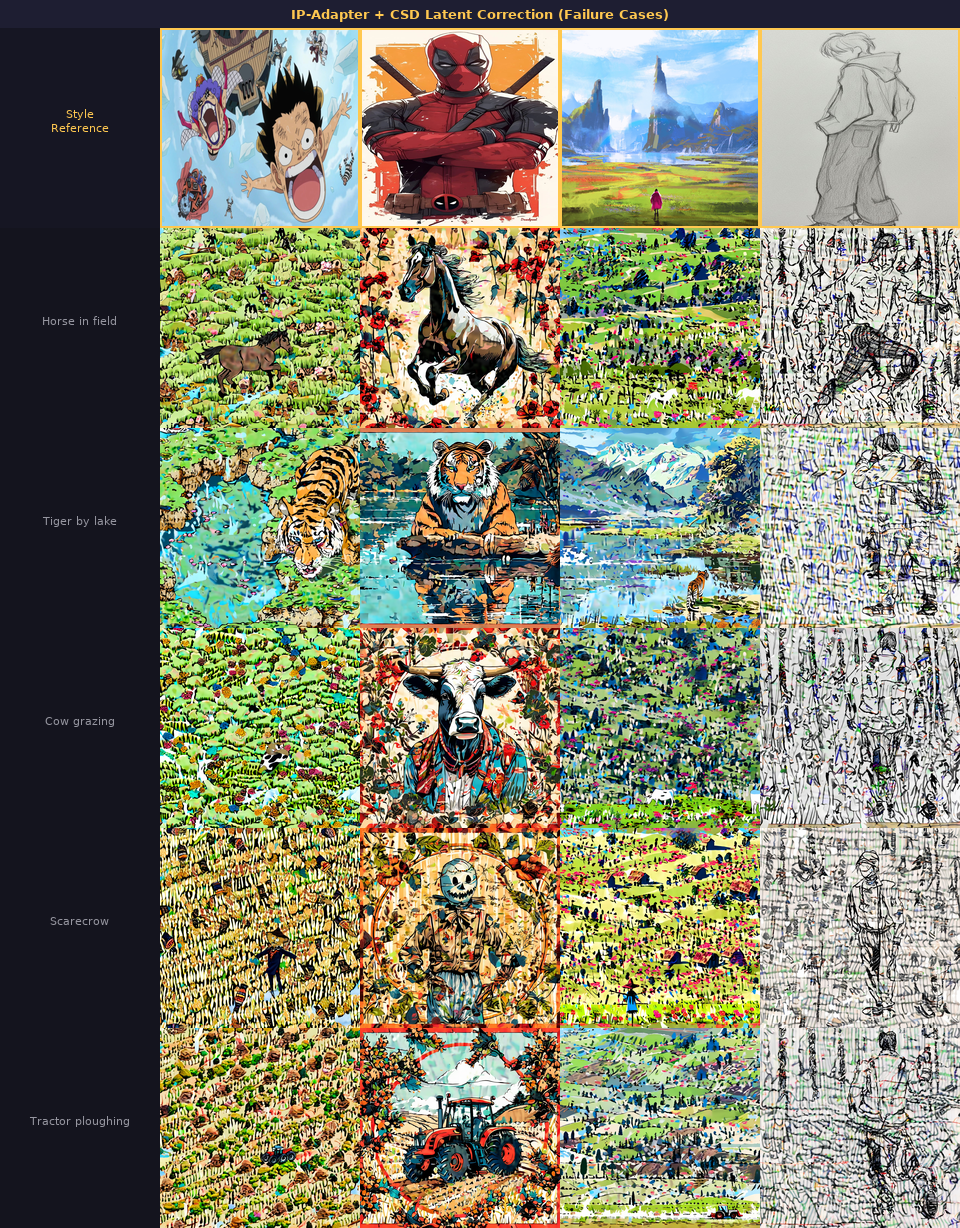
\includegraphics[width=0.88\linewidth, height=0.82\textheight, keepaspectratio]{images/ch7_grid_ipadapter_csd.png}
    \caption{IP-Adapter + unconstrained CSD latent correction across all style domains (seed 42). The first row shows the style reference for each domain. The collapse is universal — every prompt and every style produces incoherent tiled artefacts, confirming that the failure is a fundamental consequence of unconstrained latent correction rather than a style-specific issue. These failure modes directly motivate the constrained and stochastic optimisation strategies presented in Sections~\ref{sec:ch7_langevin}--\ref{sec:ch7_pld}.}
    \label{fig:ch7_grid_ipadapter_csd}
\end{figure}

\FloatBarrier
\subsection{Variable Guidance Schedules}
\label{sec:ch7_schedules}

One of the most important findings of the investigation was about the timing of optimization updates in denoising.

In early experiments, the style guidance was applied uniformly throughout the reverse diffusion process. This approach increased the style similarity, but often disturbed the formation of the semantic structure. Foreground objects were distorted, the scene composition degraded and the generated images sometimes collapsed towards the reference style image.

Later experiments used variable guidance schedules, where the strength of optimization was a function of the denoising progress. These schedules were motivated by the observation that early diffusion steps are mainly responsible for determining scene structure, while later steps refine appearance-level details.

The results consistently showed the superiority of late-stage guidance in terms of the trade-off between style fidelity and content preservation. In the last steps of the denoising process, strong optimization improved the atmospheric characteristics while preserving the semantic consistency.

\begin{figure}[htbp]
    \centering
    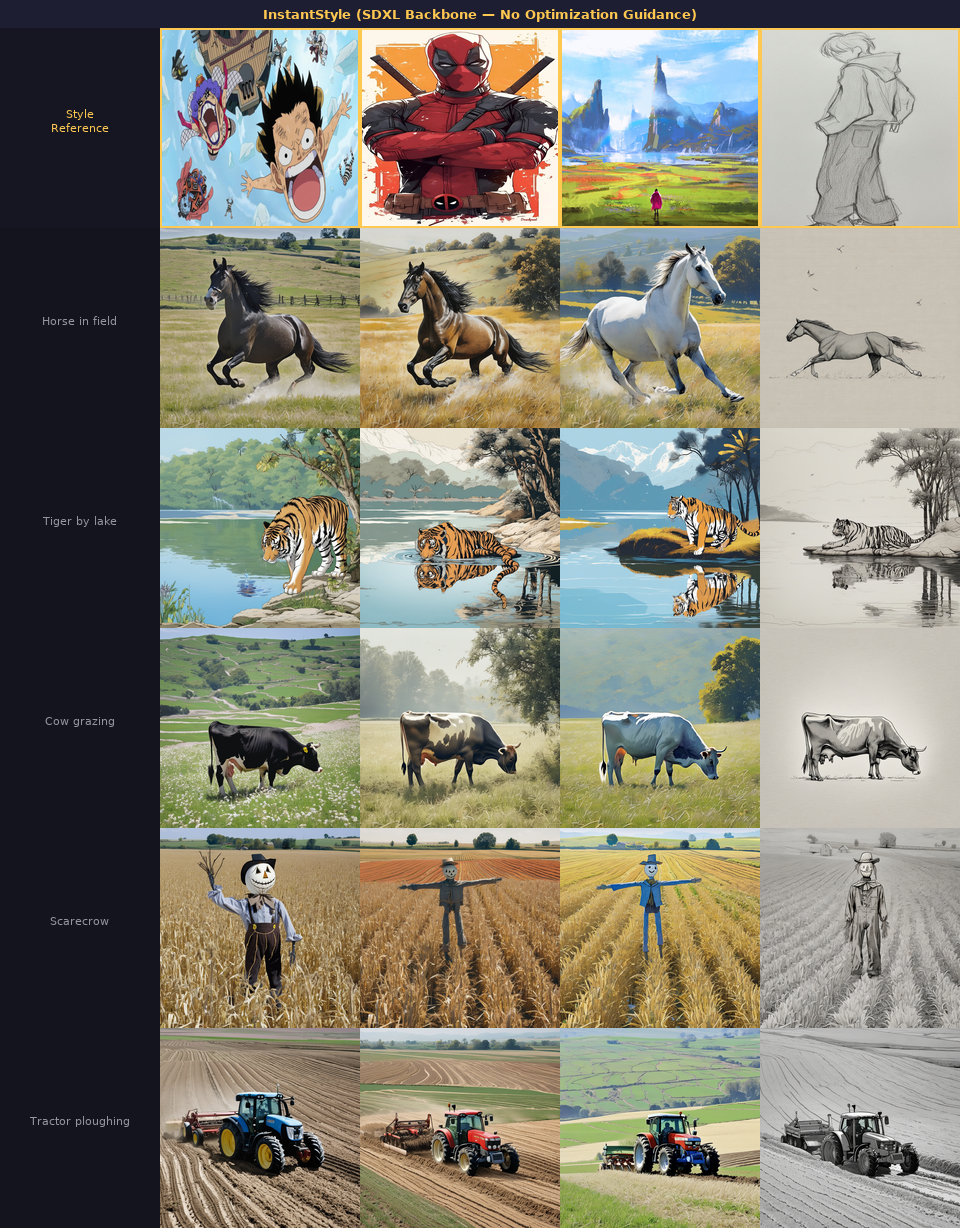
\includegraphics[width=0.95\linewidth]{images/ch7_grid_is_baseline.png}
    \caption{InstantStyle (SDXL backbone) clean feed-forward baseline grid — seed 42. The first row shows the style reference for each domain. This establishes the quality ceiling of the SDXL backbone with style injection but without any optimisation guidance; subsequent figures in this section should be read relative to this baseline.}
    \label{fig:ch7_grid_is_baseline}
\end{figure}

\begin{figure}[htbp]
    \centering
    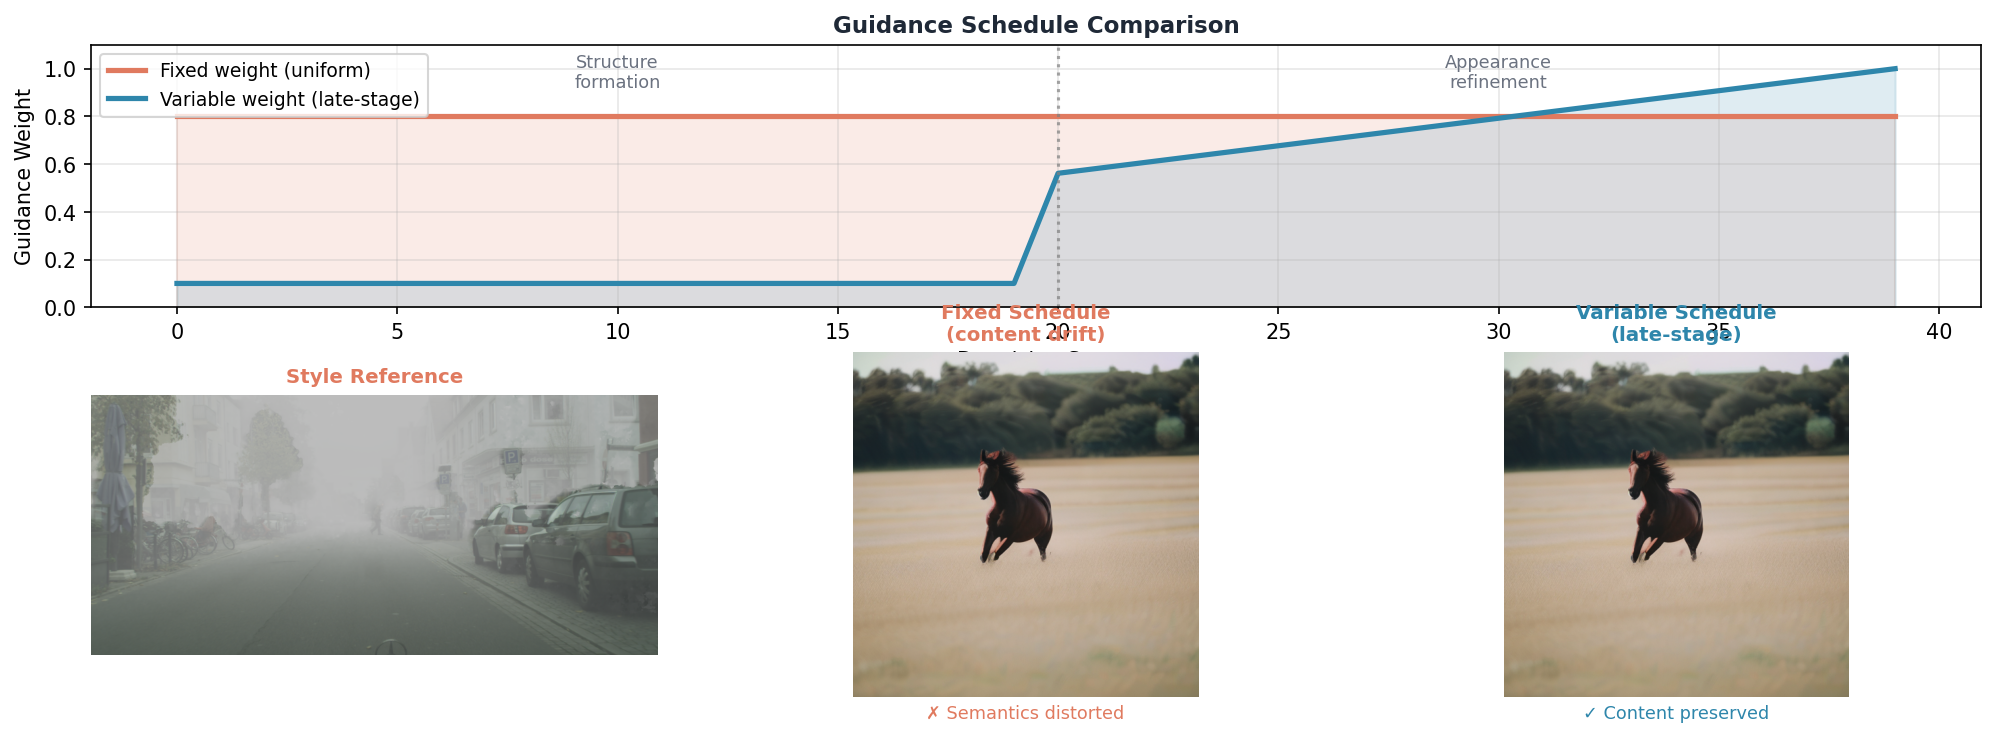
\includegraphics[width=0.95\linewidth]{images/ch7_fixed_vs_variable.png}
    \caption{Fixed versus variable guidance schedules. Late-stage optimization preserves the semantic content and allows for stronger atmospheric transformations.}
    \label{fig:fixed_vs_variable_weights}
\end{figure}

\FloatBarrier
\subsection{Case Studies: Fog Style Transfer}
\label{sec:ch7_casestudies}

To assess the developed framework on the target atmospheric domain, a focused evaluation on fog style transfer was conducted. Fog is a particularly challenging condition: it suppresses high-frequency information, degrades scene visibility, and requires depth-dependent contrast attenuation rather than a simple global colour shift. Optimisation-guided diffusion consistently generated more convincing fog effects than standard feed-forward conditioning, with the advantage most pronounced when frequency-domain constraints were included in the guidance objective.

\begin{figure}[htbp]
    \centering
    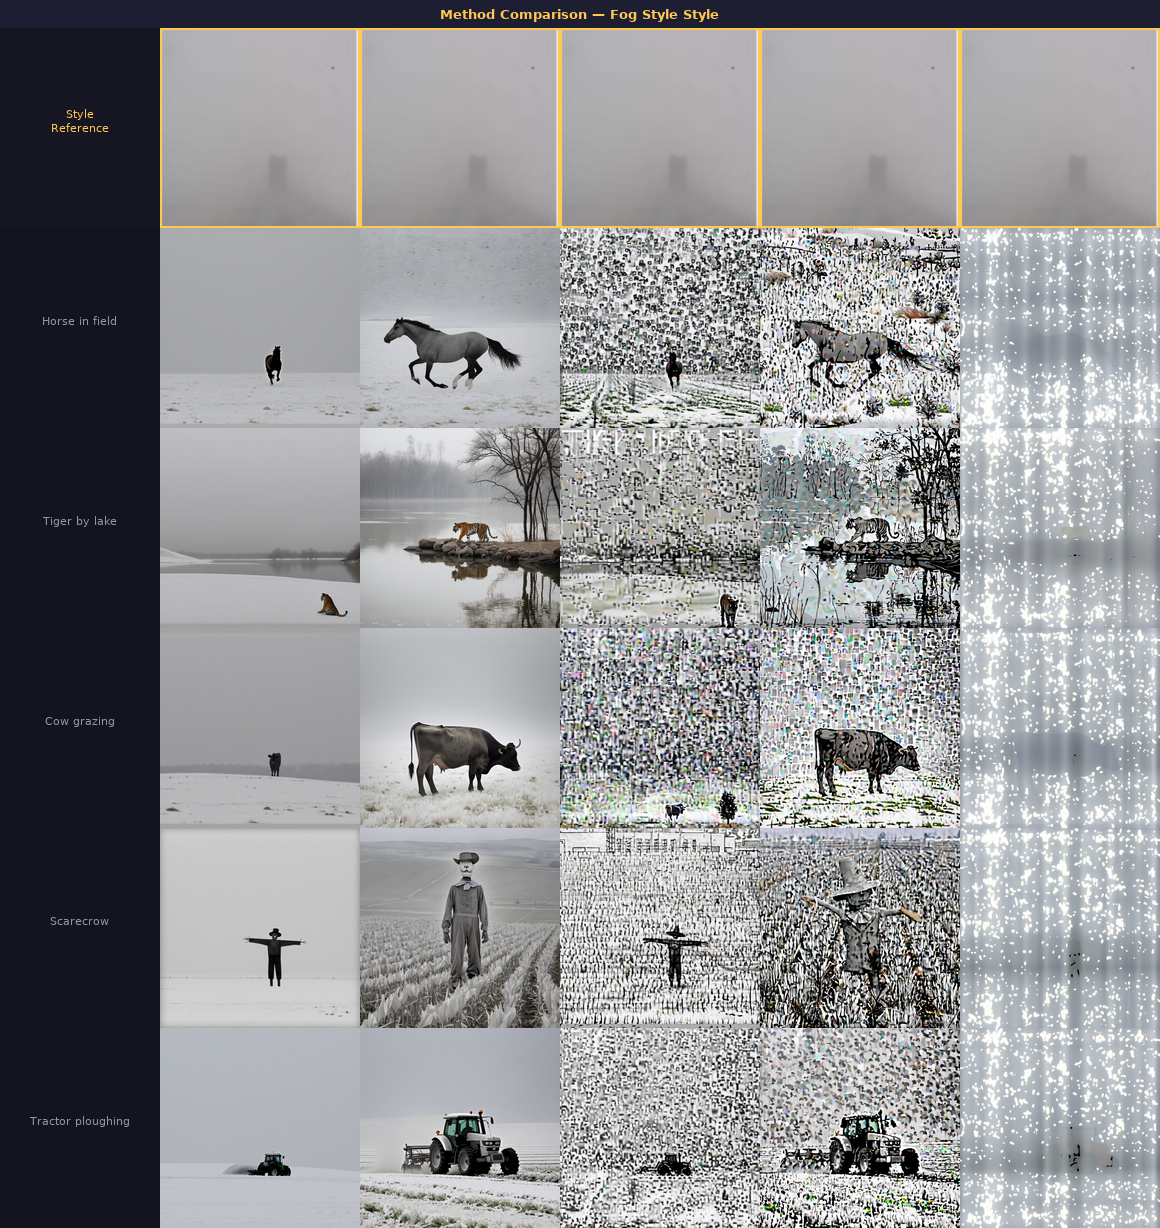
\includegraphics[width=0.95\linewidth]{images/ch7_grid_comparison.png}
    \caption{Multi-method comparison for fog atmospheric style transfer (seed 42). The first row shows the fog style reference image repeated across all method columns so the reader can judge each method against the same target; subsequent rows show generated outputs per content prompt. Columns compare IP-Adapter and InstantStyle baselines against their CSD and frequency-guided extensions, illustrating the trade-off between style fidelity and content preservation.}
    \label{fig:ch7_grid_comparison}
\end{figure}

\begin{figure}[htbp]
    \centering
    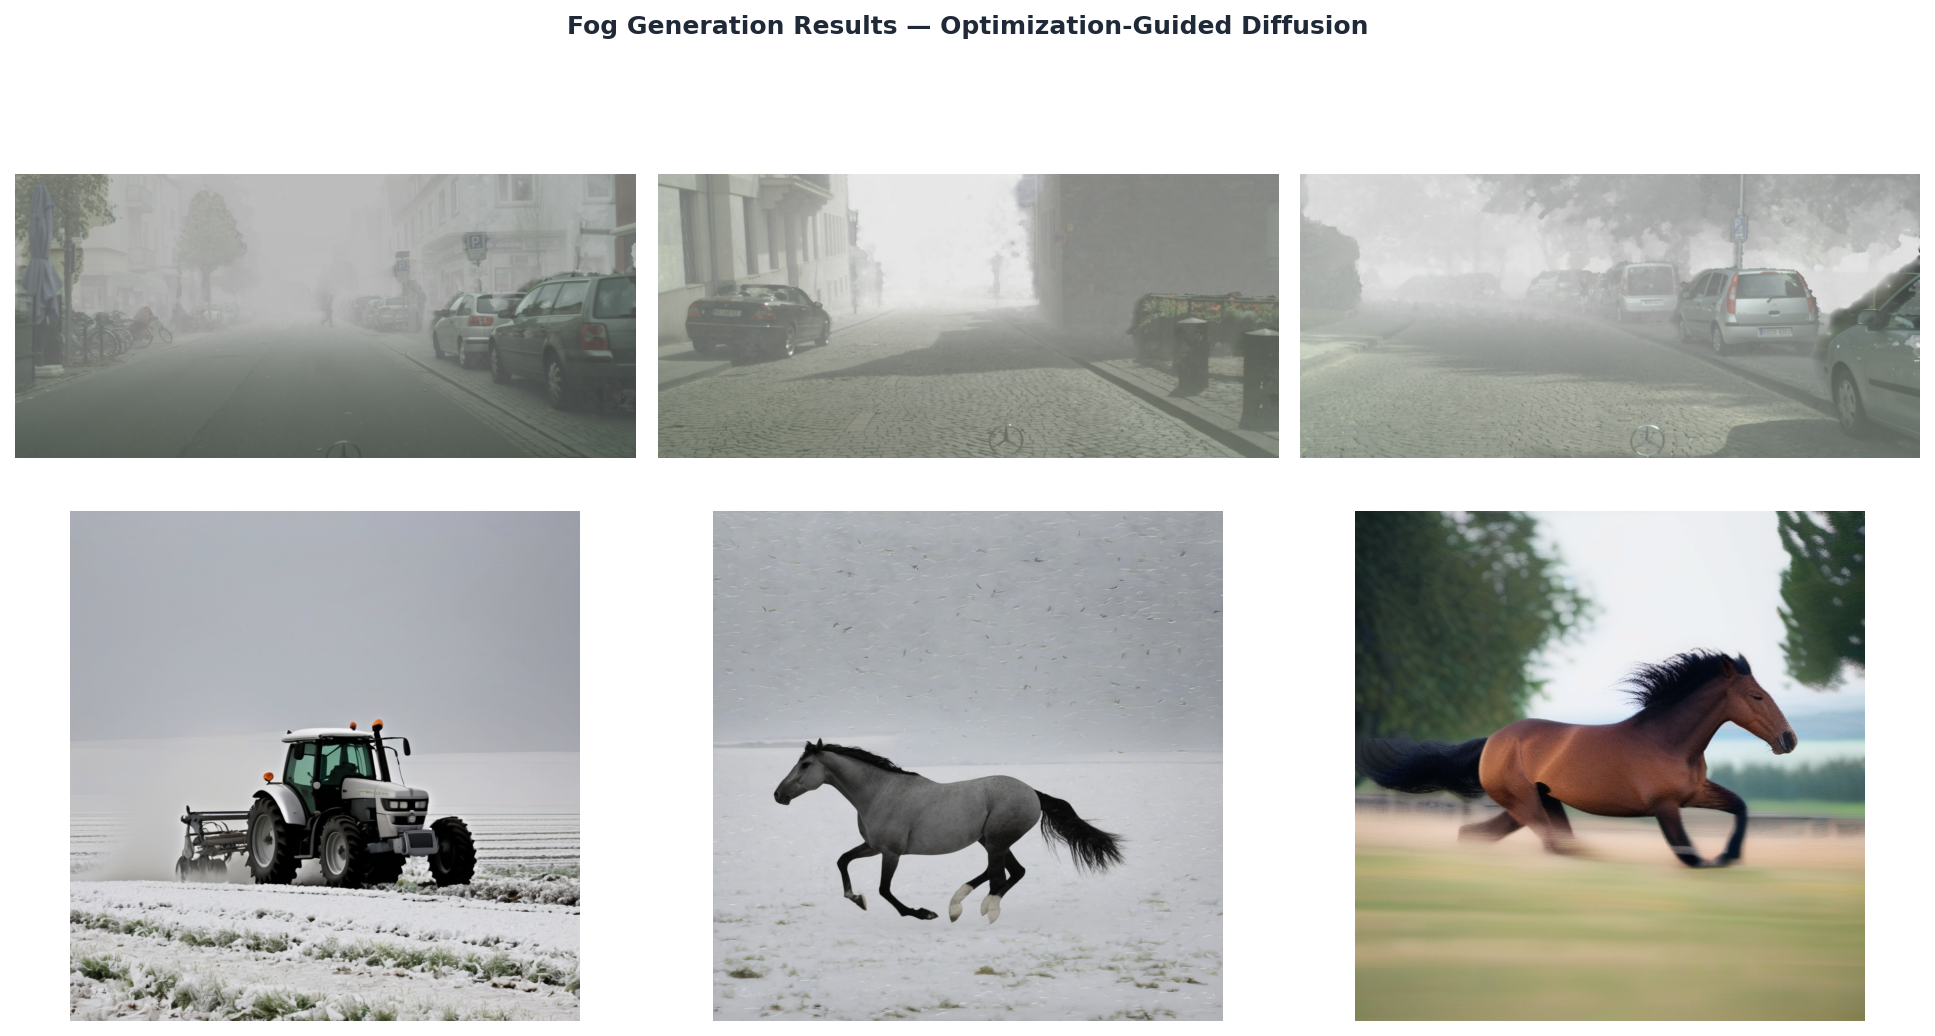
\includegraphics[width=0.95\linewidth]{images/ch7_fog_results.png}
    \caption{Representative results of fog generation via optimization-guided diffusion. Variable-weight schedule with frequency constraints produces realistic depth-dependent fog.}
    \label{fig:fog_style_results}
\end{figure}

\FloatBarrier
\subsection{Key Observations}
\label{sec:ch7_observations}

The experimental investigation yielded several important observations:

\begin{itemize}
    \item Style optimization is more effective when applied to later denoising steps.
    \item The atmospheric appearance is not representable with embedding-space similarity alone.
    \item Perceptual and frequency-domain constraints provide complementary information for better style fidelity.
    \item SDXL provides significant optimization stability improvements over Stable Diffusion 1.5.
    \item Unconstrained latent correction does not perform as well as proximal optimization strategies.
    \item Spectral guidance can be derived from the unique frequency characteristics of atmospheric phenomena.
\end{itemize}

These results collectively suggest that atmospheric style transfer can be framed as a constrained optimization problem in the reverse diffusion process. Further, they illustrate that good atmospheric guidance is obtained by combining semantic, perceptual and frequency-aware objectives, instead of depending on a single style representation.

\begin{table}[htbp]
\centering
\caption{Summary of key observations from the optimization-guided diffusion study.}
\label{tab:chapter7_findings}
\renewcommand{\arraystretch}{1.3}
\begin{tabular}{p{5.5cm} p{7.5cm}}
\toprule
\textbf{Observation} & \textbf{Consequence} \\
\midrule
Late-stage guidance is more effective & Changes atmospheric form while preserving semantic structure \\
SDXL $>$ SD1.5 & Better optimization stability with richer latent representations \\
Perceptual losses improve realism & Atmospheric effects beyond embedding similarity \\
Atmospheric phenomena have characteristic spectral signatures & FFT losses improve atmospheric fidelity \\
Proximal Langevin is more stable & Constrained optimization outperforms unconstrained updates \\
\bottomrule
\end{tabular}
\end{table}

\FloatBarrier
% =====================================================
\section{Summary}
\label{sec:ch7_summary}

This chapter explored optimisation-guided diffusion as an alternative atmospheric style transfer paradigm. Unlike traditional feed-forward style transfer methods that inject style information via conditioning mechanisms and rely solely on the diffusion model to interpret the given guidance, optimisation-guided diffusion introduces explicit objectives that are continuously enforced during the reverse diffusion process. This formulation transforms atmospheric style transfer from a passive conditioning problem into an active optimisation problem, where generated samples can be iteratively refined toward a target atmospheric distribution.

The investigation builds upon the constrained stable diffusion framework~\cite{zampini2025constrained}, which provides a generic mechanism for injecting user-specified objectives into the denoising process without modifying the diffusion model. Within this framework, Contrastive Style Descriptors (CSD)~\cite{somepalli2024csd} were studied as a style-aware representation for quantifying the atmospheric resemblance of generated images relative to style reference samples. Style losses computed on CSD embeddings were subsequently incorporated into the reverse diffusion process through latent-space optimisation.

Initial experiments showed that embedding-space guidance can successfully influence atmospheric appearance. However, the resulting optimisation process proved highly sensitive to hyperparameter selection and often exhibited unstable behaviour under strong guidance signals. These observations motivated the investigation of more principled optimisation strategies based on Langevin dynamics and Proximal Langevin dynamics. Stochastic latent refinement improved controllability and enabled stronger atmospheric transformations, but unconstrained updates frequently led to semantic degradation and reduced image quality. The introduction of proximal operators provided a more principled mechanism for balancing style adherence and fidelity to the diffusion prior, yielding substantially improved generation stability.

One important outcome of the investigation is that atmospheric appearance cannot be sufficiently described by embedding similarity alone. Global image statistics and frequency-domain properties govern atmospheric phenomena such as fog, haze, smoke, snowfall, and underwater environments in ways not captured by semantic style embeddings. This observation led to the integration of perceptual and frequency-aware objectives into the optimisation framework. Perceptual losses improved structural consistency and content preservation. Frequency-domain constraints provided a direct mechanism for modelling visibility degradation and the high-frequency attenuation characteristic of adverse environmental conditions.

The experimental progression produced several important findings. Optimisation-based guidance is far more effective when applied to later denoising steps, where appearance-level refinements dominate image formation. SDXL proved markedly more robust to optimisation-based interventions than Stable Diffusion 1.5, yielding enhanced image quality and more stable atmospheric transformations. Perceptual and spectral objectives consistently outperformed embedding-space similarity alone, confirming that atmospheric style is a fundamentally multi-faceted phenomenon requiring complementary representations. Constrained optimisation frameworks such as Proximal Langevin dynamics produced more reliable results than unconstrained latent correction strategies.

Although some experimental configurations did not yield stable results, the investigation produced valuable insights into the relationship between style representations, optimisation objectives, and diffusion-based image synthesis. The key conclusion is that atmospheric style transfer can be formulated as a constrained optimisation problem in the reverse diffusion process, and that explicit style objectives can guide generation without retraining the diffusion model.

These findings have direct implications for the physics-grounded synthesis framework presented in the following chapter. The limitations of purely embedding-based guidance and the importance of physically meaningful atmospheric representations motivated the development of a three-stage pipeline that combines depth estimation, atmospheric scattering models, and structured style injection to generate environmental transformations that are both visually convincing and physically consistent with real-world atmospheric phenomena.

% =====================================================
\chapter{Conclusions and Future Directions}
\label{chap:conclusion}

% =====================================================
\section{Conclusions}
\label{sec:conclusions}

\noindent This thesis studied the problem of atmospheric image synthesis for the purpose of generating realistic environmental domain shifts for computer vision systems. The motivation behind this research stems from a fundamental challenge of modern visual recognition models: although remarkable performance has been achieved under controlled conditions, systems are often degraded significantly when applied in adverse environmental settings. Fog, haze, sandstorms, snowfall, and underwater degradation are some atmospheric phenomena that change visibility, contrast, colour distributions, and texture statistics of scenes, resulting in complex distribution shifts that are still difficult to handle with conventional training paradigms. Collecting atmospheric datasets at a large scale is also expensive and logistically difficult, particularly for rare or hazardous environmental conditions. These observations motivate the development of methods for synthetic atmospheric data generation that can generate realistic and diverse weather-induced domain shifts.

\noindent The main goal of this thesis was to investigate whether recent advances in diffusion-based generative models can be leveraged to generate realistic atmospheric datasets that are not only visually plausible, but also induce meaningful representation-level changes in modern vision systems. Instead of concentrating on a single approach to atmospheric generation, the research investigated multiple complementary perspectives of atmospheric synthesis, progressing from purely appearance-based methods to physically motivated image formation approaches.

\noindent In the first stage of the research, atmospheric generation was investigated using diffusion-based style transfer. Modern image generation models have shown remarkable capabilities for artistic style transfer, illumination condition modification, and scene appearance change while preserving semantic content. The thesis built on these advances to explore whether atmospheric conditions could be treated as transferable visual styles. Multiple approaches were evaluated, including InstantStyle, StyleShot, and other diffusion-based frameworks, across several atmospheric settings. The proposed method for this stage --- \textbf{V0 (InstantStyle with CSD Guidance)} --- combined block-selective IP-Adapter injection with a Contrastive Style Descriptor latent correction loop, achieving the lowest CLIP confidence (0.514 ViT-L-14) of any style transfer method evaluated. Experiments showed that diffusion models are very capable of replicating weather-specific visual features such as colour shifts, contrast attenuation, and environmental textures. The atmospheric changes produced by these methods were often visually convincing and showed a great degree of stylistic agreement with the weather reference images.

\noindent The style-transfer experiments, however, also revealed fundamental limitations. While atmospheric appearance could be successfully reproduced, the induced effects were often physically inconsistent. Visibility loss was generally uniform across the entire image, independent of the distance of objects from the camera. Foreground objects remained unrealistically sharp, and the atmospheric effect resembled an overlay rather than a genuine environmental effect. These observations suggested that atmospheric conditions cannot be fully characterised by image style alone. Unlike artistic styles, atmospheric effects are sensitive to scene geometry, depth, light transport, and the physics of the environment. Purely appearance-based transfer methods, although effective at visual modification, turned out to be insufficient for modelling the underlying mechanisms of atmospheric image formation.

\noindent Inspired by these findings, the second phase of the research investigated optimization-guided diffusion as a means to explicitly include atmospheric constraints during the generation process. Atmospheric synthesis was reformulated as a constrained optimization problem, with style-aware objectives embedded directly into the reverse diffusion path. The work involved Contrastive Style Descriptors, Constrained Stable Diffusion, Langevin Dynamics, and Proximal Langevin Dynamics. These experiments yielded useful insights into the controllability of diffusion models and showed that atmospheric appearance can be guided by explicit optimization objectives rather than relying solely on feed-forward conditioning.

\noindent The optimization-guided experiments uncovered significant findings. First, they showed that atmospheric style can be imposed throughout the generation process, not only at initialization. Second, they emphasised the importance of guidance scheduling: optimizing in later denoising steps generally leads to a better trade-off between style fidelity and content preservation. Third, important limitations of embedding-space similarity objectives were identified. Semantic style embeddings do not fully capture the unique frequency and perceptual characteristics of atmospheric phenomena. Investigation of perceptual and frequency-aware objectives confirmed a more general conclusion: realistic atmospheric synthesis requires representations that incorporate physically meaningful image properties, not only visual similarity.

\noindent Optimization-guided diffusion improved controllability and enabled deeper insight into the atmospheric generation process, but also revealed the increasing complexity of trying to learn atmospheric physics implicitly through generative models. This realization motivated the final stage of the thesis. Instead of training diffusion models to learn the entire atmospheric image formation process from data, the research investigated the integration of explicit physical models into the synthesis pipeline.

\noindent This transition resulted in the development of the physics-grounded atmospheric synthesis framework presented in Chapter~\ref{chap:phase2_pipeline}. The proposed architecture was derived from knowledge acquired in prior experimental studies. The framework does not treat atmospheric generation as a single monolithic task, but breaks the problem into three independent stages: semantic scene generation, atmospheric appearance transfer, and physical image formation. Clean agricultural scenes are first generated with SDXL~\cite{podell2023sdxlimprovinglatentdiffusion}. Atmospheric characteristics are then introduced with InstantStyle~\cite{wang2024instantstyle} and IP-Adapter~\cite{ye2023ipadapterfidelityadapters} guidance. Finally, physically meaningful environmental effects are enforced with depth-aware atmospheric compositing based on the Koschmieder scattering model~\cite{koschmieder1924theorie}.

\noindent One of the most important contributions of this thesis is the recognition that semantic content generation and atmospheric generation should be treated as separate problems. Previous architectures were prone to semantic leakage, content drift, and instability when weather information and scene content were controlled jointly. The proposed framework decouples these processes, achieving substantially improved controllability by enabling atmospheric transformations to be applied without compromising scene structure or object identity. This architectural insight was key to the success of the final system.

\noindent Explicit atmospheric physics further altered the nature of the generated outputs. Unlike style-transfer approaches that only modify appearance, the physics-based compositor introduced depth-dependent visibility degradation, accumulation of atmospheric light, and weather-specific scattering behaviour. Refinements for sandstorms, snowfall, and snow accumulation demonstrated that different atmospheric phenomena have distinct physical characteristics that cannot be adequately represented by generic image transformations. The inclusion of weather-specific physical models was therefore an important factor in achieving realistic atmospheric synthesis.

\noindent The quantitative results obtained throughout the thesis offer strong evidence for the effectiveness of this approach. CLIP-based confidence analysis showed consistent decreases in classifier confidence when evaluated on generated atmospheric images, confirming significant distribution shifts at the representation level. \textbf{V9 (CLIP content subtraction + extended block injection + Koschmieder compositing) achieved the lowest confidence of any method across the entire study (0.228 ViT-L-14 / 0.227 ViT-H-14)}, establishing it as the best overall configuration and the most effective method for creating out-of-distribution atmospheric training data. Linear probing experiments demonstrated that the generated datasets contain meaningful atmospheric structure that can support downstream learning tasks. The distribution-specificity tests revealed an important observation: atmospheric adaptation is highly dependent on the properties of the generated distribution. This suggests that dataset generation methods can be as important for robustness under environmental shift as model architecture.

\noindent The results taken together support a broader conclusion about atmospheric image synthesis. Atmospheric generation should not be viewed purely as a style-transfer problem, nor purely as an optimization problem. Appearance, geometry, and physics work together to form realistic atmospheric synthesis. Diffusion models provide a powerful mechanism to generate semantically rich and visually plausible imagery, while explicit image formation models provide the physical structure necessary for realistic environmental transformations. The best atmospheric synthesis systems will likely integrate the advantages of both approaches rather than relying on one alone.

% =====================================================
\section{Future Work}
\label{sec:future_work}

\noindent The investigations presented in this thesis open several promising directions for future research. While the proposed atmospheric synthesis framework successfully integrates diffusion-based generation, style-guided transfer, and physics-grounded image formation, it also highlights opportunities to extend the realism, scalability, and applicability of synthetic atmospheric datasets.

\paragraph{Learned Atmospheric Compositors (KDA-Net and Beyond)}
The most immediate and directly motivated extension of this work is the development of a \emph{learned atmospheric compositor} to replace the hand-crafted Koschmieder stage. During the research process, an architecture named KDA-Net (Koschmieder-guided Depth-Aware Network) was prototyped: a lightweight encoder-decoder with three submodules --- a texture encoder, a haze-appearance head, and an image combiner --- trained with a combination of VGG perceptual loss and CSD contrastive loss (without adversarial training). The key insight was that classical Koschmieder compositing produces a \emph{globally smooth} depth-correlated veil that, while physically grounded, lacks the local texture irregularities present in real atmospheric images: patches of denser fog near water surfaces, scattering halos around light sources, and subject-specific depth-of-field effects. A learned compositor, trained on the output-to-reference pairs generated by the existing pipeline, could capture these sub-pixel details and produce higher-fidelity atmospheric synthesis without abandoning the depth-consistency guarantee of the physics model. The primary obstacle encountered was data volume: with only 57 real reference images in the evaluation set, the learned component was at risk of overfitting to their specific atmospheric textures. Future work with larger reference collections --- or with self-supervised objectives derived from the Koschmieder transmission law itself as a physics-regulariser --- could train a practical learned compositor that generalises across atmospheric conditions.

\paragraph{Style-Conditioned Physics Parameter Estimation}
A related but simpler learning-based direction is to replace the fixed global atmospheric parameters ($\beta$, $A$) derived from a single dark-channel prior estimate with a \emph{style-conditioned estimator} that infers per-region scattering density from the reference image. The current pipeline applies a single global $\beta$ and a single $A$ to every pixel, which approximates the atmospheric model accurately only for scenes without strong depth discontinuities. A small convolutional estimator trained to regress per-patch ($\beta$, $A$) values from style reference crops --- conditioned on depth-map statistics from DPT-Large --- could produce spatially varying atmospheric parameters and significantly improve depth-coherence in scenes with mixed near-field and far-field objects. This requires no adversarial training and could be trained on synthetic paired data generated by the existing pipeline, making it an accessible near-term extension.

\paragraph{Physics-Informed Diffusion Models}
One longer-term avenue is to build atmospheric physics directly into the diffusion process itself. In the current framework, physical image formation is a post-processing stage applied after atmospheric style transfer. This modular design provides flexibility and interpretability, but it means the diffusion model receives no physical feedback during generation --- it produces a stylised image without awareness of whether the resulting depth-attenuation profile is physically consistent. Future systems could benefit from incorporating Koschmieder-derived guidance terms directly into the reverse diffusion path: at each denoising step, a differentiable atmospheric rendering loss could nudge the predicted clean image towards configurations with depth-coherent haze. Such physics-constrained diffusion models would unify the style-transfer and compositing stages, potentially eliminating the colour-cast and content-leakage artefacts that motivated the block-selective injection and CLIP content subtraction techniques developed in this thesis.

\paragraph{Video and Temporal Consistency}
Another promising avenue is to extend the framework from image generation to video generation. In the real world, weather is inherently dynamic: fog density varies over time, snowfall has temporal structure, and sandstorms exhibit complex particle trajectories. The current framework operates on still images and does not enforce any temporal consistency. Future work could combine video diffusion models with physics-based atmospheric simulation to create temporally coherent weather sequences for testing autonomous systems in dynamic environments.

\paragraph{Compound Weather Conditions}
In this thesis, atmospheric phenomena were modelled separately, with distinct models for fog, haze, sandstorms, snowfall, and underwater environments. In practice, environmental conditions often coincide — fog with rain, snowstorms with high winds, or dust storms at sunset. Extending the framework to support multi-weather synthesis would increase realism and enable the construction of more challenging benchmark datasets.

\paragraph{Richer Atmospheric Physics}
The weather-specific refinements for sandstorms and snowstorms suggest a broader opportunity to incorporate richer atmospheric physics. The present implementation relies on simplified scattering models and heuristic accumulation mechanisms. Future work could include physically based rendering techniques, volumetric atmospheric simulation, radiative transfer models, and particle-based environmental modelling. Such approaches could substantially improve realism, especially under extreme weather conditions where multiple scattering effects are significant.

\paragraph{Adversarial Domain Shift Maximisation}
The V9 pipeline was designed and evaluated to maximise domain shift --- as measured by CLIP zero-shot confidence reduction --- using fixed pipeline parameters. A natural extension is to replace this fixed design with an adversarial optimisation loop: a \emph{generator} (the atmospheric pipeline parameterised by $\beta$, $A$, and IP-Adapter injection weights) and a \emph{discriminator} (a frozen pretrained CLIP or ViT encoder evaluating softmax confidence) are placed in competition, with the generator trained to minimise the discriminator's confidence on generated images while the discriminator remains frozen. This reduces to maximising the entropy of the classifier output over generated images --- an objective that could be optimised by differentiating through the Koschmieder compositor (which is differentiable with respect to $\beta$ and $A$) while treating the diffusion model as a black box sampled at each iteration. Preliminary experiments in this direction during the project showed that naive entropy maximisation leads to degenerate solutions (fully occluded grey images that trivially confuse any classifier); future work would need to combine entropy maximisation with a content-preservation regulariser and an image-quality prior.

\paragraph{Distribution-Aware Synthesis}
The distribution-specificity experiments in Chapter~\ref{chap:phase2_pipeline} showed that atmospheric adaptation is highly dependent on the characteristics of the generated distribution. This finding implies that dataset generation itself should be formulated as an optimisation problem. Instead of generating atmospheric images solely for visual realism, future systems could explicitly optimise synthetic datasets to maximise robustness gains for downstream tasks. Specifically, the per-class calibration failures observed in Experiments~3 and~5 --- where certain visually ambiguous categories (boar, cow) remained poorly handled even after LoRA adaptation --- suggest that a data-generation policy could be learned to over-sample the atmospheric conditions that most confuse the target model, closing the gap between visual fidelity and practical adaptation performance.

\paragraph{Broader Evaluation and Applications}
The current thesis primarily evaluated representation-level distribution shifts with vision-language models. Future work could evaluate the created datasets on a wider range of downstream tasks including object detection, semantic segmentation, instance segmentation, visual navigation, autonomous driving, agricultural monitoring, and robotic perception. Such studies would provide additional insight into the practical utility of synthetic atmospheric data across diverse application domains.

\paragraph{Domain Transfer}
The framework developed in this thesis was targeted at agricultural and rural environments. However, the underlying methodology is largely domain-independent. Future work could apply the same synthesis pipeline to urban scenes, aerial and satellite imagery, maritime environments, and indoor settings. These extensions would allow for the generation of diverse atmospheric datasets across a wide range of real-world applications.

\paragraph{Multimodal Foundation Models}
Finally, large multimodal foundation models are arriving rapidly and create new opportunities for atmospheric robustness research. Vision-language models, multimodal agents, and embodied AI systems are increasingly deployed under diverse environmental conditions. Synthetic atmospheric datasets created with frameworks such as the one proposed in this thesis could play an important role in understanding, evaluating, and improving the robustness of such next-generation systems.

\bigskip
\noindent In summary, this thesis has demonstrated that realistic atmospheric image synthesis can be achieved through a combination of diffusion-based generative modelling, optimization-based control, and physically grounded image formation principles. The research arc progresses from atmospheric style transfer through constrained diffusion to physics-aware atmospheric synthesis. The resulting framework offers a practical way to generate atmospheric datasets that produce significant environmental distribution shifts while maintaining visual realism and semantic consistency. It is hoped that the methods, insights, and findings presented in this thesis will contribute to future advances in atmospheric synthesis, domain adaptation, robustness evaluation, and the broader development of weather-aware computer vision systems.



% -------------------------------------------------------------------
% LITERATURE CITED  (section 1.7) -- follows chapters, before Acknowledgements
% -------------------------------------------------------------------
\addcontentsline{toc}{chapter}{Bibliography}
\bibliographystyle{plainnat}
\bibliography{references.bib}


\end{document}
